%for a more compact document, add the option openany to avoid
%starting all chapters on odd numbered pages
\documentclass[12pt,openany]{cmuthesis}

% This is a template for a CMU thesis.  It is 18 pages without any content :-)
% The source for this is pulled from a variety of sources and people.
% Here's a partial list of people who may or may have not contributed:
%
%        bnoble   = Brian Noble
%        caruana  = Rich Caruana
%        colohan  = Chris Colohan
%        jab      = Justin Boyan
%        josullvn = Joseph O'Sullivan
%        jrs      = Jonathan Shewchuk
%        kosak    = Corey Kosak
%        mjz      = Matt Zekauskas (mattz@cs)
%        pdinda   = Peter Dinda
%        pfr      = Patrick Riley
%        dkoes = David Koes (me)

% My main contribution is putting everything into a single class files and small
% template since I prefer this to some complicated sprawling directory tree with
% makefiles.

\definecolor{ValidRed}{rgb}{0.5,0,0}
\definecolor{TrueRed}{rgb}{1,0.6,0.2}
\definecolor{ValidBlue}{rgb}{0,0,0.5}
\definecolor{TrueBlue}{rgb}{0.2,0.6,1}

% some useful packages
\usepackage{latexsym}
\usepackage{amssymb}            % for \multimap (-o)
\usepackage{stmaryrd}           % for \binampersand (&), \bindnasrepma (\paar)

% symbols of linear logic
\newcommand{\lolli}{\multimap}
\newcommand{\tensor}{\otimes}
\newcommand{\with}{\mathbin{\binampersand}}
\newcommand{\paar}{\mathbin{\bindnasrepma}}
\newcommand{\one}{\mathbf{1}}
\newcommand{\zero}{\mathbf{0}}
\newcommand{\bang}{{!}}
\newcommand{\whynot}{{?}}
\newcommand{\bilolli}{\mathrel{\raisebox{1pt}{\ensuremath{\scriptstyle\circ}}{\lolli}}}
% \oplus, \top, \bot

% judgments of linear logic
\newcommand{\seq}[3]{{#1};{#2} \longrightarrow {#3} \mathstrut}

\newcommand{\mildrfoc}[3]{{#1};{#2} \longrightarrow [{#3}] \mathstrut}
\newcommand{\mildinv}[3]{{#1};{#2} \longrightarrow {#3} \mathstrut}
\newcommand{\mildlfoc}[4]{{#1};{#2}, [{#3}] \longrightarrow {#4} \mathstrut}


\newcommand{\urfoc}[3]{{#1};{#2} \longrightarrow [{#3}] \mathstrut}
\newcommand{\ulfoc}[4]{{#1};{#2} \,[#3] \longrightarrow {#4} \mathstrut}
\newcommand{\uinv}[4]{{#1};{#2};{#3} \longrightarrow {#4} \mathstrut}

\newcommand{\stableR}[1]{{#1}\,\mathit{stable_R} \mathstrut}
\newcommand{\stableL}[1]{{#1}\,\mathit{stable_L} \mathstrut}

\draftstamp{\today}{DRAFT}

% \usepackage{titlesec,minitoc}  
% \titleclass{\part}{top}
% \titleformat{\part}
% {\centering\normalfont\Huge\bfseries} 
% {Foo} 
% {0pt} 
% {Bar}


\begin {document} 
\frontmatter

%initialize page style, so contents come out right (see bot) -mjz
\pagestyle{empty}

\title{ %% {\it \huge Thesis Proposal}\\
{\bf Substructural Logical Specifications}}
\author{Robert J. Simmons}
\date{The Future}
\Year{Year In The Future}
\trnumber{CMU-CS-THE-FUTURE}

\committee{
Frank Pfenning, Chair \\
Robert Harper \\
Andr{\'e} Platzer \\
Iliano Cervesato, Carnegie Mellon Qatar \\
Dale Miller, INRIA-Saclay \& LIX/Ecole Polytechnique
}

\support{}
\disclaimer{}

% copyright notice generated automatically from Year and author.
% permission added if \permission{} given.

\keywords{Stuff, More Stuff}

\maketitle

% XXX MAKE DEDICATION
% \begin{dedication}
% For my dog
% \end{dedication}

\pagestyle{plain} % for toc, was empty

%% Obviously, it's probably a good idea to break the various sections of your thesis
%% into different files and input them into this file...

% XXX MAKE ABSTRACT
% \begin{abstract}
% A short summary.
% \end{abstract}

% XXX MAKE ACKNOLWEDGEMENTS
% \begin{acknowledgments}
% My advisor is cool.
% \end{acknowledgments}



\tableofcontents
\listoffigures % XXX Do I want this?
% \listoftables XXX Probably don't need this at all.

\mainmatter

%% Double space document for easy review:
%\renewcommand{\baselinestretch}{1.66}\normalsize

% The other requirements Catherine has:
%
%  - avoid large margins.  She wants the thesis to use fewer pages, 
%    especially if it requires colour printing.
%
%  - The thesis should be formatted for double-sided printing.  This
%    means that all chapters, acknowledgements, table of contents, etc.
%    should start on odd numbered (right facing) pages.
%
%  - You need to use the department standard tech report title page.  I
%    have tried to ensure that the title page here conforms to this
%    standard.
%
%  - Use a nice serif font, such as Times Roman.  Sans serif looks bad.
%
% Other than that, just make it look good...


% Introduction
\chapter{Introduction}

\section{Modular and non-modular specification}
\label{sec:modularnonmodular}

(This can mostly come out of the thesis proposal, but use 
natural semantics instead of SOS.)

\section{Substructural logical specifications}

\section{Substructural operational semantics}
\label{sec:intro-ssos}

\section{Invariants in substructural logic}


\part{Substructural logic}

% Linear logic
\chapter{Linear logic}
\label{chapter-foc}

In this chapter, we present linear logic as a logic with the ability
to express aspects of state and state transition in a natural way.  In
Chapter~\ref{chapter-order} 
we will repeat the development in this chapter in a much
richer and more expressive setting, and in Chapter~\ref{chapter-framework} 
we will carve out
a fragment of this logic to use as the basis of \sls, our logical
framework of substructural logical specifications. These three
chapters contribute to the overall thesis by focusing on the design
of logical frameworks:

\smallskip
\begin{quote} {\bf Thesis (Part I):} {\it The methodology of
    structural focalization facilitates the derivation of logical
    frameworks as fragments of focused logics.}
\end{quote}
\smallskip

\noindent
The purpose of this chapter is to introduce the methodology of
{\it structural focalization};
this development is one of the major contributions of this work. 
Linear logic is a fairly simple logic that nevertheless allows us to
consider many of the issues that will arise in richer substructural
logics like the one considered in Chapter~\ref{chapter-order}.

In Section~\ref{sec:introlinlog} we motivate and discuss a traditional
account of linear logic, and in
Section~\ref{sec:linlogicalframeworks} we discuss why this account is
insufficient as a {\it logical framework} -- derivations in linear
logic suffice to establish the existence of a series of state
transitions but do not adequately capture the structure of those
transitions. Our remedy for this insufficiency comes in the form of
{\it focusing}, Andreoli's restricted normal form for derivations in
linear logic. We discuss focusing for a polarized presentation of
linear logic in Section~\ref{sec:foclinlog}.

With focusing, we can describe {\it synthetic inference rules}
(Section~\ref{sec:linsynthetic}) that succinctly capture the structure
of focused transitions. In Section~\ref{sec:linhack} we discuss a
number of ways of modifying the design of our focused logic to
increase the expressiveness of synthetic inference rules; one of the
alternatives we present, the introduction of {\it permeable atomic
  propositions}, will be generalized and incorporated into the focused
presentation of ordered linear lax logic that we discuss in 
Chapter~\ref{chapter-order}.

% In Section~\ref{sec:linconcurrenteq}, we describe {\it concurrent
%   equality}, an equivalence relation on focused derivations introduced
% by Watkins et al.~that is motivated by the desire to capture
% independent concurrent transitions. We also discuss the limitations of
% concurrent equality in a fully focused setting.  
% In Chapter~\ref{chapter-framework}, when we
% select a fragment of ordered linear lax logic to form \sls, we will
% incorporate a similar notion of concurrent equality.


\section{Introduction to linear logic}
\label{sec:introlinlog}

Logic as it has been traditionally understood and studied -- both in
its classical and intuitionistic varieties -- treats the truth of a
proposition as a {\it persistent resource}. That is, if we have
evidence for the truth of a proposition, we can ignore that evidence
if it is not needed and reuse the evidence as many times as we need
to. Throughout this document, ``logic as it has been traditionally
understood as studied'' will be referred to as {\it persistent} logic
to emphasize this treatment of evidence. 

Linear logic, which was studied and popularized by Girard
\cite{girard87linear}, treats evidence as an {\it ephemeral} resource;
the use of an ephemeral resource consumes it, at which point it is
unavailable for further use.  Linear logic, like persistent logic,
comes in classical and intuitionistic flavors. We will favor
intuitionistic linear logic in part because the propositions of
intuitionistic linear logic (written $A$, $B$, $C$, \ldots) have a
more natural correspondence with our physical intuitions about
consumable resources. Linear conjunction $A \tensor B$ (``$A$ tensor
$B$'') represents the resource built from the resources $A$ and $B$;
if you have both a bowl of soup {\it and} a sandwich, that resource
can be represented by the proposition ${\sf soup} \otimes {\sf
  sandwich}$. Linear implication $A \lolli B$ (``$A$ lolli $B$'')
represents a resource that can interact with another resource $A$ to
produce a resource $B$. One robot with batteries not included could be
represented as the linear resource $({\sf battery} \lolli {\sf
  robot})$, and the linear resource $({\sf 6bucks} \lolli {\sf soup}
\tensor {\sf sandwich})$ represents the ability to use \$6 to obtain
lunch -- but only once.\footnote{Conjunction will always bind more
  tightly than implication, so this is equivalent to the proposition
  ${\sf 6bucks} \lolli ({\sf soup} \tensor {\sf sandwich})$.} Linear
logic also has a connective ${!}A$ (``bang $A$'' or ``of course $A$'')
representing a persistent resource that can be used to generate any
number of $A$ resources, including zero. Your local Panera, which
allows six dollars to be exchanged for both soup and a sandwich any
number of times, can be represented as the resource ${!}({\sf 6bucks}
\lolli {\sf soup} \tensor {\sf sandwich})$.

\begin{figure}[t]
\begin{tabbing}
\quad $A$ \,\, \=  
   $::= p \mid {!}A \mid \one \mid A \tensor B \mid A \lolli B$\\
\quad $\Gamma$ \> $::= \cdot \mid \Gamma, A$ \qquad \= {\it (multiset)}\\
\quad $\Delta$ \> $::= \cdot \mid \Delta, A$ \> {\it (multiset)}\\
\end{tabbing}
%
%
\quad \fbox{$\seq{\Gamma}{\Delta}{A}$}
\[
\infer[{\it id}]
{\seq{\Gamma}{p}{p}}
{}
\qquad
\infer[{\it copy}]
{\seq{\Gamma, A}{\Delta}{C}}
{\seq{\Gamma, A}{\Delta, A}{C}}
%
\]

\[
%
\infer[{!}_R]
{\seq{\Gamma}{\cdot}{{!}A}}
{\seq{\Gamma}{\cdot}{A}}
\qquad
\infer[{!}_L]
{\seq{\Gamma}{\Delta, {!}A}{C}}
{\seq{\Gamma, A}{\Delta}{C}}
\qquad
\infer[\one_R]
{\seq{\Gamma}{\cdot}{\one}}
{}
\qquad
\infer[\one_L]
{\seq{\Gamma}{\Delta, \one}{C}}
{\seq{\Gamma}{\Delta}{C}}
\]

\[
%
\infer[{\tensor}_R]
{\seq{\Gamma}{\Delta_1,\Delta_2}{A \tensor B}}
{\seq{\Gamma}{\Delta_1}{A}
 &
 \seq{\Gamma}{\Delta_2}{B}}
\qquad
\infer[{\tensor}_L]
{\seq{\Gamma}{\Delta, A \tensor B}{C}}
{\seq{\Gamma}{\Delta, A, B}{C}}
\]

\[
%
\infer[{\lolli}_R]
{\seq{\Gamma}{\Delta}{A \lolli B}}
{\seq{\Gamma}{\Delta, A}{B}}
\qquad
\infer[{\lolli}_L]
{\seq{\Gamma}{\Delta_1,\Delta_2, A \lolli B}{C}}
{\seq{\Gamma}{\Delta_1}{A}
 &
 \seq{\Gamma}{\Delta_2, B}{C}}
%
\]
\caption{Intuitionstic linear logic}
\label{fig:linear}
\end{figure}


Figure~\ref{fig:linear} presents a standard sequent calculus for
linear logic, in particular the {\it multiplicative, exponential}
fragment of intuitionistic linear logic (or {\it MELL}), so called
because the connectives $\one$, $A \tensor B$, and $A \lolli B$ are
considered to be the {\it multiplicative} connectives, and the
connective ${!}A$ is the {\it exponential} connective of
intuitionistic linear logic.\footnote{In this chapter we will mostly
  ignore the {\it additive} connectives of intuitionistic linear logic
  $\zero$, $A \oplus B$, $\top$, and $A \with B$ and will entirely
  ignore the {\it first-order} connectives $\exists x.A$ and $\forall
  x.A$. The ``why not'' connective $\mbox{?}A$ from classical linear
  logic is sometimes treated as a second exponential connective in
  intuitionistic linear logic \cite{chang03judgmental}, but we will
  never ask ``why not?'' in the context of this dissertation.} It
corresponds most closely to Barber's dual intuitionistic linear logic
\cite{barber96dual}, but also to Andreoli's dyadic system
\cite{andreoli92logic} and Chang et al.'s judgmental analysis of
intuitionistic linear logic \cite{chang03judgmental}.

%\subsection{Transitions in linear logic}
%\label{sec:linlogtrans}

The propositions of intuitionistic linear logic, and linear implication
in particular, capture a notion of state change: we can {\it
  transition} from a state where we have both a ${\sf battery}$ and
the battery-less robot (represented, as before, by the linear
implication ${\sf battery} \lolli {\sf robot}$) to a state where we
have the battery-endowed (and therefore presumably functional) robot
(represented by the proposition ${\sf robot}$). In other words, the
proposition
%
\[{\sf battery} \otimes ({\sf battery} \lolli {\sf robot}) \lolli
{\sf robot}\] 
%
is provable in linear logic. These transitions can be chained
together as well: if we start out with ${\sf
  6bucks}$ instead of ${\sf battery}$ but we also have the
persistent ability to turn ${\sf 6bucks}$ into a ${\sf battery}$ --
just like we turned \$6 into a bowl of soup and a salad at Panera --
then we can ultimately get our working robot as well.
Written as a series of transitions, the picture looks like this:
\[
\begin{array}{ccccc}
\begin{array}{c}
\mbox{\it \$6 (1)}\medskip\\ 
\mbox{\it battery-less robot (1)} \medskip\\ 
\mbox{\it turn \$6 into a battery}\\
\mbox{\it (all you want)}
\end{array}
& \leadsto &
\begin{array}{c}
\mbox{\it battery  (1)}\medskip\\ 
\mbox{\it battery-less robot (1)} \medskip\\ 
\mbox{\it turn \$6 into a battery}\\
\mbox{\it (all you want)}
\end{array}
& \leadsto &
\begin{array}{c}
\mbox{\it robot (1)} \medskip\\ 
\mbox{\it turn \$6 into a battery}\\
\mbox{\it (all you want)}\medskip\\~\\
\end{array}
\end{array}
\]
In linear logic, these transitions correspond to the provability
of the proposition
\[{!}({\sf 6bucks} \lolli {\sf battery}) \otimes {\sf 6bucks} \otimes
({\sf battery} \lolli {\sf robot}) \lolli {\sf robot}.\] A derivation
of this proposition is given in
Figure~\ref{fig:unfocused-robot}.\footnote{In
  Chapter~\ref{chapter-framework} (and Section~\ref{sec:whytraces} in
  particular) we see that this view isn't quite precise enough, and
  that the ``best'' representation of state change from the state
  $A$ to the state $B$ isn't really captured by derivations of the
  proposition $A \lolli B$ or by derivations of the sequent
  $\seq{\cdot}{A}{B}$.  However, this view remains a simple and useful
  one; Cervesato and Scedrov cover it thoroughly in the context of
  intuitionistic linear logic \cite{cervesato09relating}.}

\begin{figure}
\[
\infer[{\lolli}_R]
{\seq{\cdot}{\cdot}{{!}({\sf 6bucks} \lolli {\sf battery}) \otimes
                    {\sf 6bucks} \otimes 
                    ({\sf battery} \lolli {\sf robot}) \lolli {\sf robot}}}
{\infer[{\otimes}_L]
{\seq{\cdot}{{!}({\sf 6bucks} \lolli {\sf battery}) \otimes
                    {\sf 6bucks} \otimes 
                    ({\sf battery} \lolli {\sf robot})}{{\sf robot}}}
{\infer[{!}_L]
{\seq{\cdot}{{!}({\sf 6bucks} \lolli {\sf battery}),
                    {\sf 6bucks} \otimes 
                    ({\sf battery} \lolli {\sf robot})}{{\sf robot}}}
{\infer[{\otimes}_L]
{\seq{\Gamma}{{\sf 6bucks} \otimes 
                    ({\sf battery} \lolli {\sf robot})}{{\sf robot}}}
{\infer[{\lolli}_L]
{\seq{\Gamma}{{\sf 6bucks}, {\sf battery} \lolli {\sf robot}}{{\sf robot}}}
{\infer[{\it copy}]
 {\seq{\Gamma}{{\sf 6bucks}}{{\sf battery}}}
 {\infer[{\lolli}_L] 
  {\seq{\Gamma}{{\sf 6bucks}, {\sf 6bucks} \lolli {\sf battery}}{{\sf battery}}}
  {\infer[{\it init}]
   {\seq{\Gamma}{{\sf 6bucks}}{{\sf 6bucks}}}
   {}
   &
   \infer[{\it init}]
   {\seq{\Gamma}{{\sf battery}}{{\sf battery}}}
   {}}}
 &
 \infer[{\it init}]
 {\seq{\Gamma}{{\sf robot}}{{\sf robot}}}
 {}}}}}}
\] 
\caption{Proving that a transition is possible 
(where we let $\Gamma = {\sf 6bucks} \lolli {\sf battery}$).}
\label{fig:unfocused-robot}
\end{figure}


It is precisely because linear logic contains this intuitive notion of
state and state transition that a rich line of work, dating back to
Chirmar's 1995 dissertation, has sought to use linear logic as a {\it
  logical framework} for describing stateful systems
\cite{chirimar95proof,cervesato02linear,
  cervesato02concurrent,pfenning04substructural,miller09formalizing,
  pfenning09substructural,cervesato09relating}.  

\section{Logical frameworks}
\label{sec:linlogicalframeworks}

Generally speaking, logical frameworks use the {\it structure} of
proofs in a logic (like linear logic) to describe the structures we're
interested in (like the process of obtaining a robot).  There are two
related reasons why linear logic as described in
Figure~\ref{fig:linear} is not immediately useful as a logical
framework. First, the structure of the derivation in
Figure~\ref{fig:unfocused-robot} doesn't really match the intuitive
two-step transition that we sketched out above. Second, there are {\it
  lots} of derivations of our example proposition according to the
rules in Figure~\ref{fig:linear}, even though there's only one
``real'' series of transitions that get us to a working robot. The use
of ${!}L$, for instance, could be permuted up past the ${\otimes}L$
and then past the ${\lolli}L$ into the left branch of the proof. These
differences represent inessential nondeterminism in proof construction
-- they just get in the way of the structure that we are trying to
capture.

This is a general problem in the construction of logical frameworks.
We'll discuss two solutions in the context of LF, a logical
framework based on dependent type theory that has proved to be a
suitable means of encoding a wide variety of deductive systems, such
as logics and programming languages \cite{harper93framework}.  The
first solution is to define an appropriate equivalence class of
proofs, and the second solution is to define a complete set
of canonical proofs.

Defining an appropriate equivalence relation on proofs can be an effective
way of handling this inessential nondeterminism.  In
linear logic as presented above, if the permutability of rules like
${!}_L$ and ${\otimes}_L$ is problematic, we can instead reason about
{\it equivalence classes} of derivations. Derivations that differ only
in the ordering of ${!}_L$ and ${\otimes}_L$ rules belong in the
same equivalence class (which means we treat them as equivalent):
\[
\infer[{!}_L]
{\seq{\Gamma}{\Delta, {!}A, B \otimes C}{D}}
{\infer[{\otimes}_L]
 {\seq{\Gamma,A}{\Delta, B \otimes C}{D}}
 {\deduce{\seq{\Gamma,A}{\Delta, B, C}{D}}{\mathcal D}}}
\quad
\deduce{\mathstrut}{\mathstrut{\equiv}}
\quad
\infer[{\otimes}_L]
{\seq{\Gamma}{\Delta, {!}A, B \otimes C}{D}}
{\infer[{!}_L]
 {\seq{\Gamma}{\Delta, {!}A, B, C}{D}}
 {\deduce{\seq{\Gamma,A}{\Delta, B, C}{D}}{\mathcal D}}}
\]

In LF, lambda calculus terms (which correspond to derivations by the
Curry-Howard correspondence) are considered modulo the least
equivalence class that includes
\begin{itemize}
\item $\alpha$-equivalence ($\lambda x.N \equiv \lambda y.N[y/x]$ if 
$y \not\in {\it FV}(N)$), 
\item $\beta$-equivalence 
($(\lambda x.\,M)N \equiv M[N/x]$ if $x \not\in {\it FV}(N)$), and 
\item $\eta$-equivalence ($N \equiv \lambda x.N\,x$).
\end{itemize}
The weak normalization property for LF establishes that, given any
typed LF term, we can find an equivalent term that is $\beta$-normal
(no $\beta$-redexes of the form $(\lambda x.M) N$ exist) and
$\eta$-long (replacing $N$ with $\lambda x.N\,x$ anywhere would
introduce a $\beta$-redex or make the term ill-typed).  
In any given equivalence class of typed LF terms, all the
$\beta$-normal and $\eta$-long terms are $\alpha$-equivalent.
Therefore, because $\alpha$-equivalence is decidable, the equivalence
of typed LF terms is  decidable. 

The uniqueness of $\beta$-normal and $\eta$-long terms within an
equivalence class of lambda calculus terms (modulo
$\alpha$-equivalence, which we will henceforth take for granted) makes
these terms useful as canonical representatives of equivalence
classes. In Harper, Honsell, and Plotkin's original formulation
of LF, a deductive system is said to be {\it adequately encoded} as
an LF type family in the case that there is a compositional bijection
between the formal objects in the deductive system and these
$\beta$-normal, $\eta$-long representatives of equivalence classes
\cite{harper93framework}, a topic we will return to in 
Section~\ref{sec:lf-adequacy}.

Modern presentations of LF, such as Harper and Licata's
\cite{harper07mechanizing}, follow the approach developed by Watkins
et al.~\cite{watkins02concurrent} and define the logical framework so
that it only contains these $\beta$-normal, $\eta$-long {\it canonical
  forms} of LF. This presentation of LF is called Canonical LF to
distinguish it from the original presentation of LF in which the
$\beta$-normal, $\eta$-long terms are just a refinement of terms. A
central component in this approach is {\it hereditary substitution};
in Chapter~\ref{chapter-ordered}, we will make the connections between
hereditary substitution and the focused cut admissibility property we
prove in this chapter more explicit.  Hereditary substitution also
establishes a normalization property for LF. Using hereditary
substitution we can easily take a regular LF term and transform it
into a Canonical LF term. By a separate theorem, we can prove that the
normalized term will be equivalent to the original term
\cite{martens12lf}. %\footnote{This process is the same as the way we use cut
%  admissibility to prove cut elimination.} 
 % An important point is that the normalization theorem we prove
% this way is a strictly weaker theorem than so-called weak
% normalization -- it does not, a priori, imply that the .

Our analogue to the canonical forms of LF will be the {\it focused
  derivations} of linear logic that are presented in the next
section. In Section~\ref{sec:foclinlog} below, we will present 
focused linear logic and see that there is exactly 
one focused derivation that derives the proposition
\[{!}({\sf 6bucks} \lolli {\sf battery}) \otimes {\sf 6bucks} \otimes
({\sf battery} \lolli {\sf robot}) \lolli {\sf robot}.\] 
%
We will furthermore see that the structure of this derivation matches
the intuitive transition interpretation, a point
that is reinforced by the discussion of {\it synthetic inference
  rules} in Section~\ref{sec:linsynthetic}. 

\section{Focused linear logic}
\label{sec:foclinlog}

Andreoli's original motivation for introducing focusing was not to
describe a logical framework, it was to describe a foundational logic
programming paradigm based on proof search in classical linear logic
\cite{andreoli92logic}. The existence of multiple proofs that differ
in inessential ways is particularly problematic for proof search, as
inessential differences between derivations correspond to unnecessary
choice points that a proof search procedure will need to backtrack
over. 

The development in this section introduces {\it structural
  focalization}, a methodology for deriving the correctness of a
focused sequent calculus (Theorem~\ref{thm:linfocsound} and
Theorem~\ref{thm:linfoccomplete}, Section~\ref{sec:lincorrectness}) as
a consequence of the internal completeness (identity expansion,
Theorem~\ref{thm:linidentity}, Section~\ref{sec:linindentity}) and
internal soundness (cut admissibility, Theorem~\ref{thm:lincut},
Section~\ref{sec:lincut}) of the focused system. This
methodology is a substantial refinement of the method used by
Chaudhuri to establish the correctness of focused intuitionistic
linear logic \cite{chaudhuri06focused}, and because it relies on
structural methods, structural focalization is more amenable to
mechanized proof \cite{simmons11structural}.  Our focused sequent
calculus also departs from Chaudhuri's by treating asynchronous rules
as confluent rather than fixed, a point that will be discussed in
Section~\ref{sec:confluent-v-fixed}.

\subsection{Polarity}
\label{sec:linpolar}

The first step in describing a focused sequent calculus is to classify
connectives into two groups \cite{andreoli92logic}.  Some connectives,
such as linear implication $A \lolli B$, are called {\it asynchronous}
because their right rules can always be applied eagerly, without
backtracking, during bottom-up proof search. Other connectives, such
as multiplicative conjunction $A \tensor B$, are called {\it
  synchronous} because their right rules cannot be applied
eagerly. For instance, if we are trying to prove the sequent $A
\tensor B \longrightarrow B \tensor A$, the ${\tensor}R$ rule cannot
be applied eagerly; we first have to decompose $A \tensor B$ on the
left using the ${\tensor}L$ rule.  The terms asynchronous and
synchronous make a bit more sense in a one-sided classical sequent
calculus; in intuitionistic logics, it is common to call asynchronous
connectives {\it right}-asynchronous and {\it
  left}-synchronous. Similarly, it is common to call synchronous
connectives {\it right}-synchronous and {\it left}-asynchronous.  We
will instead use a different designation, calling the
(right-)synchronous connectives {\it positive} (${!}$, $\zero$, $\oplus$,
$\one$, and $\otimes$ in full propositional linear logic) and calling
the (right-)asynchronous connectives {\it negative} ($\lolli$, $\top$
and $\with$ in full propositional linear logic); this assignment is
called the proposition's {\it polarity}. Each atomic proposition must
be assigned to have only one polarity, though this assignment can be
made arbitrarily.

The nontrivial result of focusing is that it is possible to separate a
proof into two strictly alternating phases. In {\it inversion} phases,
positive propositions on the left and negative propositions on the
right are eagerly and exhaustively decomposed using invertible
rules.\footnote{Synchronicity or polarity, a property of connectives,
  is closely connected to (and sometimes conflated with) a property of
  rules called {\it invertibility}; a rule is invertible if the
  conclusion of the rule implies the premises. So ${\lolli}R$ is
  invertible ($\seq{\Gamma}{\Delta}{A \lolli B}$ implies
  $\seq{\Gamma}{\Delta, A}{B}$) but ${\lolli}L$ is not
  ($\seq{\Gamma}{\Delta, A \lolli B}{C}$ does not imply that $\Delta =
  \Delta_1, \Delta_2$ such that $\seq{\Gamma}{\Delta_1}{A}$ and
  $\seq{\Gamma}{\Delta_2, B}{C}$).  Rules that can be applied eagerly
  need to be invertible, so asynchronous connectives have invertible
  right rules and synchronous connectives have invertible left
  rules. Therefore, in the literature a common synonym for
  asynchronous/negative is {\it right-invertible}, and the analogous
  synonym for synchronous/positive is {\it left-invertible}.}  In {\it
  focused} phases, a single proposition is selected (the proposition
{\it in focus}, which is either a positive proposition in right focus
or a negative proposition in left focus). This
proposition is then decomposed repeatedly and
exhaustively using rules that are mostly non-invertible.

If we consider this discipline applied to our robot example where all
atoms have been assigned positive polarity, we would begin with an
inversion phase, decomposing the negative implication on the right and
the positive tensor and exponential on the left:
\[
\infer[{\lolli}_R]
{\seq{\cdot}{\cdot}{{!}({\sf 6bucks} \lolli {\sf battery}) \otimes
                    {\sf 6bucks} \otimes 
                    ({\sf battery} \lolli {\sf robot}) \lolli {\sf robot}}}
{\infer[{\otimes}_L]
{\seq{\cdot}{{!}({\sf 6bucks} \lolli {\sf battery}) \otimes
                    {\sf 6bucks} \otimes 
                    ({\sf battery} \lolli {\sf robot})}{{\sf robot}}}
{\infer[{!}_L]
{\seq{\cdot}{{!}({\sf 6bucks} \lolli {\sf battery}),
                    {\sf 6bucks} \otimes 
                    ({\sf battery} \lolli {\sf robot})}{{\sf robot}}}
{\infer[{\otimes}_L]
{\seq{{\sf 6bucks} \lolli {\sf battery}}{{\sf 6bucks} \otimes 
                    ({\sf battery} \lolli {\sf robot})}{{\sf robot}}}
{\deduce
{\seq{{\sf 6bucks} \lolli {\sf battery}}{{\sf 6bucks}, 
                    {\sf battery} \lolli {\sf robot}}{{\sf robot}}}
{\vdots}}}}}
\]
Once we reach the topmost sequent in the above fragment, we have to
pick a negative proposition on the left or a positive proposition on
the right as our focus in order to proceed. The correct choice in this
context is to pick the negative proposition ${\sf 6bucks} \lolli {\sf
  battery}$ in the persistent context and decompose it using the
non-invertible rule ${\lolli}_L$. Because the subformula ${\sf
  6bucks}$ is positive and ends up on the right side in the
subderivation, the focusing discipline requires that we prove it
immediately with the ${\it id}$ rule. Letting $\Gamma = {\sf 6bucks}
\lolli {\sf battery}$, this looks like this:
\[
\infer[{\it copy}]
{\deduce[\vdots]{}{\seq{\Gamma}{{\sf 6bucks}, 
                    {\sf battery} \lolli {\sf robot}}{{\sf robot}}}}
{\infer[{\lolli}_L]
{\seq{\Gamma}{{\sf 6bucks}, 
                    {\sf battery} \lolli {\sf robot}, 
   {\sf 6bucks} \lolli {\sf battery}}{{\sf robot}}}
{\infer[{\it id}]
 {\seq{\Gamma}{{\sf 6bucks}}{{\sf 6bucks}}}
 {}
 &
 \deduce
 {\seq{\Gamma}{{\sf battery} \lolli {\sf robot}, 
   {\sf battery}}{{\sf robot}}}
 {\vdots}}}
\]
The trace (that is, the pair of a single bottom sequent and 
a set of unproved top sequents) of an inversion phase stacked
on top of a
focused phase is called a {\it synthetic
  inference rule} by Chaudhuri, a point we will return to in
Section~\ref{sec:linsynthetic}.

\subsection{Polarization}

At this point, there is an important choice to make. One way forward
is to treat positive and negative propositions as syntactic
refinements of the set of all propositions, and to develop a focused
presentation for intuitionistic linear logic with the connectives and
propositions that we have already considered, as Chaudhuri did in
\cite{chaudhuri06focused}.  The other way forward is to treat positive
and negative propositions as distinct syntactic classes $A^+$ and
$A^-$ with explicit inclusions, called {\it shifts}, between them.
This is called {\it polarized} linear logic.  The positive proposition
${\downarrow}A^-$, pronounced ``downshift $A$'' or ``down $A$,'' has a
subterm that is a negative proposition; the negative proposition
${\uparrow}A^+$, pronounced ``upshift $A$'' or ``up $A$,'' has a
subterm that is a positive proposition.
\begin{align*}
A^+ & ::= p^+ \mid {\downarrow}A^- \mid {!}A^- \mid \one \mid A^+ \tensor B^+\\
A^- & ::= p^- \mid {\uparrow}A^+ \mid A^+ \lolli B^-
\end{align*}

\begin{figure}
{\small \[
\begin{array}{rcl|rcl|rcl}
({\downarrow}A^-)^\circ & \!\!\!=\!\!\! & (A^-)^\circ & & & & & & 
\\
(p^+)^\circ & \!\!\!=\!\!\! & p^+ &
(p^+)^\oplus & \!\!\!=\!\!\! & p^+ &
(p^+)^\ominus & \!\!\!=\!\!\! & {\uparrow}p^+
\\
({!}A^-)^\circ & \!\!\!=\!\!\! & {!}(A^-)^\circ &
({!}A)^\oplus & \!\!\!=\!\!\! & {!}A^\ominus &
({!}A)^\ominus & \!\!\!=\!\!\! & {\uparrow}({!}A^\ominus)
\\
(\one)^\circ & \!\!\!=\!\!\! & \one &
(\one)^\oplus & \!\!\!=\!\!\! & \one &
(\one)^\ominus & \!\!\!=\!\!\! & {\uparrow}\one 
\\
(A^+ \otimes B^+)^\circ & \!\!\!=\!\!\! & (A^+)^\circ \otimes (B^+)^\circ &
(A \otimes B)^\oplus & \!\!\!=\!\!\! & A^\oplus \otimes B^\oplus &
(A \otimes B)^\ominus & \!\!\!=\!\!\! & {\uparrow}(A^\oplus \otimes B^\oplus)
\\
({\uparrow}A^+)^\circ & \!\!\!=\!\!\! & (A^+)^\circ & & & & & & 
\\
(p^-)^\circ & \!\!\!=\!\!\! & p^- &
(p^-)^\oplus & \!\!\!=\!\!\! & {\downarrow}p^- &
(p^-)^\ominus & \!\!\!=\!\!\! & p^- 
\\
(A^+ \lolli B^-)^\circ & \!\!\!=\!\!\! & (A^+)^\circ \lolli (B^-)^\circ &
(A \lolli B)^\oplus & \!\!\!=\!\!\! & {\downarrow}(A^\oplus \lolli B^\ominus) &
(A \lolli B)^\ominus & \!\!\!=\!\!\! & A^\oplus \lolli B^\ominus
\end{array}
\]}

\caption{Polarizing and de-polarizing propositions of MELL.}
\label{fig:lin-shift}
\end{figure}


The relationship between unpolarized and polarized linear logic is
given by two erasure functions $(A^+)^\circ$ and $(A^-)^\circ$ that
wipe away all the shifts; this function is defined in
Figure~\ref{fig:lin-shift}. In the other direction, every proposition
in unpolarized linear logic has an polarized analogue with a minimal
number of shifts, given by the functions $A^\oplus$ and $A^\ominus$
in Figure~\ref{fig:lin-shift}.  Both of these functions are partial
inverses of erasure, since $(A^\oplus)^\circ = (A^\ominus)^\circ = A$;
we will generally refer to partial inverses of erasure as {\it
  polarization strategies}. The strategies $A^\oplus$ and $A^\ominus$
are minimal, avoiding shifts wherever possible, but there are many
other possible strategies, such as the fully-shifting strategy that
always adds either one or two shifts between every connective, which
we can write as $(A)^{m+} = B^+$ and $(A)^{m-} = B^-$, defined in
Figure~\ref{fig:lin-maxshift}.

\begin{figure}
{\small \[
\begin{array}{rcl|rcl}
(p^+)^{m+} & \!\!\!=\!\!\! & {\downarrow}{\uparrow}p^+ &
(p^+)^{m-} & \!\!\!=\!\!\! & {\uparrow}p^+
\\
({!}A)^{m+} & \!\!\!=\!\!\! & {\downarrow}{\uparrow}{!}(A)^{m-} &
({!}A)^{m-} & \!\!\!=\!\!\! & {\uparrow}{!}(A)^{m-}
\\
(\one)^{m+} & \!\!\!=\!\!\! & {\downarrow}{\uparrow}\one &
(\one)^{m-} & \!\!\!=\!\!\! & {\uparrow}\one 
\\
(A \otimes B)^{m+} & \!\!\!=\!\!\!
    & {\downarrow}{\uparrow}((A)^{m+} \otimes (B)^{m+}) &
(A \otimes B)^{m-} & \!\!\!=\!\!\! & {\uparrow}(A^\oplus \otimes B^\oplus)
\\
& & & & & 
\\
(p^-)^{m+} & \!\!\!=\!\!\! & {\downarrow}p^- &
(p^-)^{m-} & \!\!\!=\!\!\! & {\uparrow}{\downarrow}p^- 
\\
(A \lolli B)^{m+} & \!\!\!=\!\!\! & {\downarrow}((A)^{m+} \lolli (B)^{m-}) &
(A \lolli B)^{m-} & \!\!\!=\!\!\!
     & {\uparrow}{\downarrow}((A)^{m+} \lolli (B)^{m-})
\end{array}
\]}

\caption{Fully-shifting polarization strategy for MELL}
\label{fig:lin-maxshift}
\end{figure}

Shifts turn out to have a profound impact on the structure of focused
proofs, though erasure requires that they have no impact on {\it
  provability}. For instance, the proofs of $A$ in Chaudhuri's focused
presentation of linear logic are isomorphic to the proofs of
$(A)^\oplus$ in the polarized logic discussed below,\footnote{This
  isomorphism holds for Chaudhuri's focused presentation of linear
  logic precisely because his treatment of atomic propositions differs
  from Andreoli's. This isomorphism does not hold relative to focused
  systems that follow Andreoli's design, a point we will return to in
  Section~\ref{sec:linhack}.} whereas the proofs of $(A)^{m+}$ in
polarized logic are isomorphic to the {\it unfocused} proofs of linear
logic as described in Figure~\ref{fig:linear}. Other polarization
strategies correspond to different focused logics, as explored by
Liang and Miller in \cite{liang09focusing}, so the presentation of
polarized linear logic below, like Liang and Miller's LJF, can be seen
in two ways: as a focused logic in its own right, and as a framework
for defining many focused logics (one per polarization strategy). As
such, the strongest statement of the correctness of focusing is based
on erasure: there is an unfocused derivation of $(A^+)^\circ$ or
$(A^-)^\circ$ if and only if there is a focused derivation of $A^+$ or
$A^-$.  Most existing proofs of the completeness of focusing only
verify a weaker property: that there is an unfocused derivation of $A$
if and only if there is a focused derivation of $A^\bullet$, where
$A^\bullet$ is some polarization strategy.  The only exception seems
to be Zeilberger's proof for classical persistent logic
\cite{zeilberger08unity}.

In this dissertation, we will be interested only in the structure of focused
proofs, which corresponds to using the polarization strategy given by
$A^\oplus$ and $A^\ominus$. Therefore, following Chaudhuri, it would
be possible to achieve our objectives without the use of polarization.
Our choice is largely based on practical
considerations: the use of polarized logic simplifies the proof of
identity expansion in Section~\ref{sec:linindentity} and the proof of
completeness in Section~\ref{sec:lincorrectness}. That said, polarized
logic is an independently significant and currently active area of
research. For instance, the Curry-Howard
interpretation of polarized persistent logic has been studied by Levy
as Call-by-Push-Value \cite{levy04call}. The erasable influence of the
shifts on the structure (but not the existence) of proofs is also
important in the context of theorem proving. For instance, a theorem
prover for polarized logic can imitate focused proof search by using
the $(A)^\oplus$ polarization strategy and unfocused proof search by
using the $(A)^{m+}$ polarization strategy
\cite{mclaughlin09efficient}.

\subsection{Focused sequent calculus}
\label{sec:linfocseqcalcdef}

Usually, focused logics are described as having multiple sequent
forms. For intuitionistic logics, there need to be at least three
sequent forms:
\smallskip
\begin{itemize}
\item $\mildrfoc{\Gamma}{\Delta}{A^+}$ (the {\it right focus} sequent, where
the proposition $A^+$ is in focus),
\item $\mildinv{\Gamma}{\Delta}{C}$ (the {\it inversion} sequent), and
\item $\mildlfoc{\Gamma}{\Delta}{A^-}{C}$ (the {\it left focus} sequent,
where the proposition $A^-$ is in focus).
\end{itemize}
\smallskip
It is also possible to distinguish a fourth sequent form, the {\it
  stable} sequents, inversion sequents $\mildinv{\Gamma}{\Delta}{C}$
where no asynchronous inversion remains to be done. A sufficient
condition for stability is that the context $\Delta$ contains only negative 
propositions
$A^-$ and the succedent $C$ is a positive proposition $A^+$.
However, this cannot be a {\it necessary} condition for stability
due to the presence of atomic propositions. 
If the process of inversion reaches a positive atomic
proposition $p^+$ on the left or a negative atomic proposition $p^-$
on the right, the proposition can be decomposed no further. When we
reach an atomic proposition, we are therefore forced to {\it suspend}
decomposition, either placing a suspended positive atomic proposition
$\susp{p^+}$ in $\Delta$ or placing a suspended negative proposition
$\susp{p^-}$ as the succedent. For technical reasons discussed below
in Section~\ref{sec:lin-suspended}, our sequent calculus can handle
arbitrary suspended propositions, not just  suspended atomic
propositions, and suspended propositions are always treated as stable,
so $\mildseq{\Gamma}{A^-, B^-, C^-}{D^+}$ and
$\mildseq{\Gamma}{\susp{A^+}, B^-, \susp{C^+}}{\susp{D^-}}$ are both
stable sequents.

Another reasonable presentation of linear logic, and the one we will
adopt in this section, uses only one sequent form,
$\mildseq{\Gamma}{\underline{\Delta}}{\underline{U}}$, that
generalizes what is allowed to appear in the linear context
$\underline{\Delta}$ or in the succedent $\underline{U}$. We will use
this interpretation to understand the logic described in
Figure~\ref{fig:kaustuv-focused}. In addition to propositions $A^+$,
$A^-$ and positive suspended positive propositions $\langle A^+ \rangle$, 
the grammar
of contexts $\underline{\Delta}$ allows them to contain left focuses
$[ A^- ]$.  Likewise, a succedent $\underline{U}$ can be a stable
positive proposition $A^+$, a suspended negative proposition
$\susp{A^-}$, a focused positive proposition $[ A^+ ]$, or an
inverting negative proposition $A^-$. We will henceforth write
$\Delta$ and $U$ to indicate the refinements of $\underline{\Delta}$
and $\underline{U}$ that do not contain any focus.

\begin{figure}[tb]
\begin{tabbing}
\quad $A^+$ \= $::= p^+ 
              \mid {\downarrow}A^- 
              \mid {!}A^- 
              \mid \one
              \mid A \otimes B$\\
\quad $A^-$ \> $::= p^-
              \mid {\uparrow}A^+
              \mid A \lolli B$\\
\quad $\Gamma$ \> $::= \cdot \mid \Gamma, A^-$ \qquad\qquad\qquad\qquad\qquad\qquad\quad \= {\it (multiset)}\\
\quad $\Delta$ \> $::= \cdot \mid \Delta, A^+ \mid \Delta, A^- \mid \Delta, [A^-] \mid \Delta, \langle A^+ \rangle$ \> {\it (multiset)}\\
\quad $U$ \> $::= A^- \mid A^+ \mid [ A^+ ] \mid \langle A^- \rangle$\\
\end{tabbing}
%
%
\quad \fbox{$\mildseq{\Gamma}{\Delta}{U}$}
\[
\infer[{\it focus}^*_R]
{\mildseq{\Gamma}{\Delta}{A^+}}
{\mildseq{\Gamma}{\Delta}{[A^+]}}
\quad
\infer[{\it focus}^*_L]
{\mildseq{\Gamma}{\Delta,A^-}{U}}
{\mildseq{\Gamma}{\Delta,[A^-]}{U}}
\quad
\infer[{\it copy}^*]
{\mildseq{\Gamma, A^-}{\Delta}{U}}
{\mildseq{\Gamma, A^-}{\Delta, [A^-]}{U}}
\]

\[
\infer[\eta^+]
{\mildseq{\Gamma}{\Delta, p^+}{U}}
{\mildseq{\Gamma}{\Delta, \langle p^+ \rangle}{U}}
\quad
\infer[{\it id}^+]
{\mildseq{\Gamma}{\langle A^+ \rangle}{[A^+]}}
{}
\quad
\infer[\eta^-]
{\mildseq{\Gamma}{\Delta}{p^-}}
{\mildseq{\Gamma}{\Delta}{\langle p^- \rangle}}
\quad
\infer[{\it id}^-]
{\mildseq{\Gamma}{[A^-]}{\langle A^- \rangle}}
{}
\]

\[
\infer[{\uparrow}_R]
{\mildseq{\Gamma}{\Delta}{{\uparrow}A^+}}
{\mildseq{\Gamma}{\Delta}{A^+}}
\quad
\infer[{\uparrow}_L]
{\mildseq{\Gamma}{\Delta, [{\uparrow}A^+]}{U}}
{\mildseq{\Gamma}{\Delta, A^+}{U}}
\quad
\infer[{\downarrow}_R]
{\mildseq{\Gamma}{\Delta}{[{\downarrow}A^-]}}
{\mildseq{\Gamma}{\Delta}{A^-}}
\quad
\infer[{\downarrow}_L]
{\mildseq{\Gamma}{\Delta, {\downarrow}A^-}{U}}
{\mildseq{\Gamma}{\Delta, A^-}{U}}
\]

\[
%
\infer[{!}_R]
{\mildseq{\Gamma}{\cdot}{[{!}A^-]}}
{\mildseq{\Gamma}{\cdot}{A^-}}
\quad
\infer[{!}_L]
{\mildseq{\Gamma}{\Delta, {!}A^-}{U}}
{\mildseq{\Gamma, A^-}{\Delta}{U}}
\quad
\infer[\one_R]
{\mildseq{\Gamma}{\cdot}{[\one]}}
{}
\quad
\infer[\one_L]
{\mildseq{\Gamma}{\Delta, \one}{U}}
{\mildseq{\Gamma}{\Delta}{U}}
\]

\[
%
\infer[{\tensor}_R]
{\mildseq{\Gamma}{\Delta_1,\Delta_2}{[A^+ \tensor B^+]}}
{\mildseq{\Gamma}{\Delta_1}{[A^+]}
 &
 \mildseq{\Gamma}{\Delta_2}{[B^+]}}
\quad
\infer[{\tensor}_L]
{\mildseq{\Gamma}{\Delta, A^+ \tensor B^+}{U}}
{\mildseq{\Gamma}{\Delta, A^+, B^+}{U}}
\]

\[
%
\infer[{\lolli}_R]
{\mildseq{\Gamma}{\Delta}{A^+ \lolli B^-}}
{\mildseq{\Gamma}{\Delta, A^+}{B^-}}
\quad
\infer[{\lolli}_L]
{\mildseq{\Gamma}{\Delta_1,\Delta_2, [A^+ \lolli B^-]}{U}}
{\mildseq{\Gamma}{\Delta_1}{[A^+]}
 &
 \mildseq{\Gamma}{\Delta_2, [B^-]}{U}}
%
\]
\caption{Focused intuitionstic linear logic.}
\label{fig:kaustuv-focused}
\end{figure}


By adding a side condition to the three rules ${\it focus}_R$, ${\it
  focus}_L$, and ${\it copy}$ that neither the context $\Delta$ nor
the succedent $U$ can contain an in-focus proposition $[A^+]$ or
$[A^-]$, derivations can maintain the invariant that there is always
at most one proposition in focus in any sequent, effectively restoring
the situation in which there are three distinct
judgments. %\footnote{Treating these extra conditions as a side
%  condition is strictly a cosmetic matter; we don't want to have to
%  write them constantly when we .}  
Therefore, from this point on, we will only consider sequents
$\mildseq{\Gamma}{\underline{\Delta}}{\underline{U}}$ with at most one
focus. Pfenning, who developed this construction in
\cite{pfenning12chaining}, calls this invariant the {\it focusing
  constraint}.
% and writes $\delta$ and $\gamma$ instead of $\underline{\Delta}$ and
% $\underline{U}$.
The focusing constraint alone gives us what Pfenning calls a {\it
  chaining} logic \cite{pfenning12chaining} and which Laurent calls a
{\it weakly focused} logic
\cite{laurent04proof}.\footnote{Unfortunately, I made the meaning of
  ``weak focusing'' less precise by calling a different sort of logic
  weakly focused in \cite{simmons11weak}.  That weakly focused system
  had an additional restriction that invertible rules could {\it not}
  be applied when any other proposition was in focus, which is what
  Laurent called a strongly $+$-focused logic.}  We obtain a fully
focused logic by further restricting the three critical rules ${\it
  focus}_R$, ${\it focus}_L$, and ${\it copy}$ so that they only apply
when the sequent below the line is stable. In light of this
additional restriction, whenever we consider a focused sequent
$\mildseq{\Gamma}{\Delta, [A^-]}{U}$ or
$\mildseq{\Gamma}{\Delta}{[A^+]}$, we can assume that $\Delta$ and $U$
are stable.

The persistent context of a focused derivation can always be weakened
by adding more persistent resources.  This weakening property can be
phrased as an admissible rule, which we indicate using a dashed line:
\[
\infer-[\it weaken]
{\mildseq{\Gamma, \Gamma'}{\underline \Delta}{\underline U}}
{\mildseq{\Gamma}{\underline \Delta}{\underline U}}
\]
In developments following Pfenning's structural cut admissibility
methodology \cite{pfenning00structural}, it is critical that the
weakening theorem {\it does not} change the structure of proofs: that the
structure of the derivation $\mildseq{\Gamma}{\underline
  \Delta}{\underline U}$ is unchanged when we weaken it to
$\mildseq{\Gamma, \Gamma'}{\underline \Delta}{\underline U}$. It turns
out that the development in this chapter does not rely on this property.
% In
% contrast, the Structural Focalization development that this chapter
% follows does not rely on this property \cite{simmons11structural}.

Suspended propositions ($\langle A^+ \rangle$ and $\langle A^-
\rangle$) and the four rules that interact with suspended propositions
(${\it id}^+$, ${\it id}^-$, $\eta^+$, and $\eta^-$) are the main
nonstandard aspect of this presentation.  The $\eta^+$ and $\eta^-$
rules, which allow us to stop decomposing a proposition that we are
eagerly decomposing with invertible rules, are restricted to atomic
propositions, and there is no other way for suspended propositions to
be introduced into the context with rules. It seems reasonable to
restrict the two rules that capture the identity principles, ${\it
  id}^+$ and ${\it id}^-$, to atomic propositions as well.  However,
the seemingly unnecessary generality of these two identity rules makes
it much easier to establish the standard metatheory of this sequent
calculus. To see why this is the case, we will turn our attention to
suspended propositions and the four admissible rules (two focal
substitution principles and two identity expansion principles) that
interact with suspended propositions.


\subsection{Suspended propositions}
\label{sec:lin-suspended}

In unfocused sequent calculi, it is generally possible to restrict the
${\it id}$ rule to atomic propositions (as shown in
Figure~\ref{fig:linear}). The general ${\it id}$ rule,
which concludes $\seq{\Gamma}{A}{A}$ for all propositions $A$, is
admissible just as the ${\it cut}$ rule is admissible. But while the
${\it cut}$ rule can be eliminated completely, the atomic ${\it id}$
rule must remain. This is related to the logical interpretation of
atomic propositions as stand-ins for unknown propositions.  All
sequent calculi, focused or unfocused, have the subformula property:
every rule breaks down a proposition, either on the left or the right
of the turnstile ``$\vdash$'', when read from bottom to top. We are
unable to break down atomic propositions any further (they are
unknown), thus the ${\it id}$ rule is necessary at atomic
propositions.  If we substitute a concrete proposition for some atomic
proposition, the structure of the proof stays exactly the same, except
that instances of initial sequents become admissible instances of the
identity theorem.

To my knowledge, all published proof systems for focused logic have
incorporated a focused version of the ${\it id}$ rule that also
applies only to atomic propositions. This treatment is not incorrect
and is obviously analogous to the ${\it id}$ rule from the unfocused
system. Nevertheless, I believe this to be a design error, and it is
one that has historically made it unnecessarily difficult to prove the
identity theorem for focused systems. The alternative developed in
this chapter is the use of suspensions. Suspended positive
propositions $\langle A^+ \rangle$ only appear in the linear context
$\Delta$, and suspended negative propositions $\langle A^- \rangle$
only appear as succedents. They are treated as stable (we never break
down a suspended proposition) and are only used to immediately prove a
proposition in focus with one of the identity rules ${\it id}^+$ or
${\it id}^-$. The rules ${\it id}^+$ and ${\it id}^-$ are more general
focused versions of the unfocused ${\it id}$ rule. This extra
generality does not influence the structure of proofs because
suspended propositions can only be introduced into the context or the
succedent by the $\eta^+$ and $\eta^-$ rules, and those rules {\it
  are} restricted to atomic propositions.
% The restriction of these
% identity rules to suspended propositions allows us to maintain the
% structure of the logic, but the generalization of the identity rules
% to arbitrary suspended propositions g.

\paragraph{Suspended positive propositions} act much like regular variables in a
natural deduction system. The positive identity rule ${\it id}^+$
allows us to prove any positive proposition given that the positive
proposition appears suspended in the context.  There is a
corresponding substitution principle for focal substitutions that has
a natural-deduction-like flavor: we can substitute a derivation
right-focused on $A^+$ for a suspended positive proposition $\langle
A^+ \rangle$ in a context.

\bigskip
\begin{theorem}[Focal substitution (positive)]\label{thm:fsubst-pos}~\\
If $\mildseq{\Gamma}{\Delta}{[A^+]}$ 
and $\mildseq{\Gamma}{\underline{\Delta'}, \langle A^+ \rangle}
      {\underline{U}}$, 
then $\mildseq{\Gamma}{\underline{\Delta'}, \Delta}{\underline{U}}$.
\end{theorem}

\begin{proof}
  Straightforward induction over the second given derivation, as in a
  proof of regular substitution in a natural deduction system. If the
  second derivation is the axiom ${\it id}^+$, the result follows
  immediately using the first given derivation.
\end{proof}

\noindent
As discussed above in Section~\ref{sec:linfocseqcalcdef}, because we
only consider focused sequents that are otherwise stable, we assume
that $\Delta$ in the statement of Theorem~\ref{thm:fsubst-pos} is
stable by virtue of it appearing in the focused sequent
$\mildseq{\Gamma}{\Delta}{[A^+]}$. The second premise
$\mildseq{\Gamma}{\underline{\Delta'}, \langle A^+
  \rangle}{\underline{U}}$, on the other hand, may be a right-focused
sequent $\mildseq{\Gamma}{\Delta', \langle A^+ \rangle}{[B^+]}$, a
left-focused sequent $\mildseq{\Gamma}{\Delta'', [B^-], \langle A^+
  \rangle}{U}$, or an inverting sequent.

\paragraph{Suspended negative propositions} are a bit less intuitive
than suspended positive propositions. While a derivation of
$\mildseq{\Gamma}{\underline{\Delta'}, \langle A^+
  \rangle}{\underline{U}}$ is missing a premise that can be satisfied
by a derivation of $\mildseq{\Gamma}{\Delta}{[A^+]}$, a derivation of
$\mildseq{\Gamma}{\underline{\Delta}}{\langle A^- \rangle}$ is missing
a {\it continuation} that can be satisfied by a derivation of
$\mildseq{\Gamma}{\Delta', [A^-]}{U}$. The focal substitution
principle, however, still takes the basic form of a substitution
principle.

\bigskip
\begin{theorem}[Focal substitution (negative)]\label{thm:fsubst-neg}~\\
If $\mildseq{\Gamma}{\underline{\Delta}}{\langle A^- \rangle}$
and $\mildseq{\Gamma}{\Delta', [A^-]}{U}$, 
then $\mildseq{\Gamma}{\Delta', \underline{\Delta}}{U}$. 
\end{theorem}

\begin{proof}
  Straightforward induction over the {\it first} given derivation; if
  the first derivation is the axiom ${\it id}^-$, the result follows
  immediately using the second given derivation.
\end{proof}

% \noindent
% As a regular substitution principle that is inductive over the structure
% of the first given proposition, focal substitution is reminiscent of 
% the {\it leftist substitutions} introduced by Pfenning and Davies in the 
% context of the possibility modality \cite{pfenning01judgmental}.

Unlike cut admissibility, which we discuss in
Section~\ref{sec:lincut}, both of the focal substitution principles
are straightforward inductions over the structure of the derivation
containing the suspended proposition. As an aside, when we encode
%The Structural Focalization
%development \cite{simmons11structural} discusses how, when we encode
the focused sequent calculus for persistent logic in LF, a suspended
positive premise can be naturally encoded as a hypothetical right
focus. This encoding makes the ${\it id}^+$ rule an instance of the
hypothesis rule provided by LF and establishes
Theorem~\ref{thm:fsubst-pos} ``for free'' as an instance of LF
substitution. This is possible to do for negative focal substitution
as well, but it is counterintuitive and relies on a peculiar use of
LF's uniform function space \cite{simmons11structural}.

The two substitution principles can be phrased as admissible rules for
building derivations, like the ${\it weaken}$ rule above:
\[
\infer-[{\it subst}^+]
{\mildseq{\Gamma}{\underline{\Delta'}, \Delta}{\underline{U}}}
{\mildseq{\Gamma}{\Delta}{[A^+]}
 &
 \mildseq{\Gamma}{\underline{\Delta'}, \langle A^+ \rangle}{\underline{U}}}
\qquad
\infer-[{\it subst}^-]
{\mildseq{\Gamma}{\Delta', \underline{\Delta}}{U}}
{\mildseq{\Gamma}{\underline{\Delta}}{\langle A^- \rangle}
 &
 \mildseq{\Gamma}{\Delta', [A^-]}{U}}
\]

Note the way in which these admissible substitution principles
generalize the logic: ${\it subst}^+$ or ${\it subst}^-$ are the
only rules we have discussed that allow us to introduce non-atomic
suspended propositions, because only {\it atomic} suspended propositions are
introduced explicitly by rules $\eta^+$ and $\eta^-$.

\subsection{Identity expansion}
\label{sec:linindentity}

Suspended propositions appear in Figure~\ref{fig:kaustuv-focused} in
two places: in the identity rules, which we have just discussed and
connected with the focal substitution principles, and in the rules
marked $\eta^+$ and $\eta^-$, which are also the only mention of
atomic propositions in the presentation. It is here that we need to
make a critical shift of perspective from unfocused to focused
logic. In an unfocused logic, the rules nondeterministically break
down propositions, and the initial rule ${\it id}$ puts an end to this
process when an atomic proposition is reached. In a focused logic, the
focus and inversion phases must break down a proposition {\it all the
  way} until a shift is reached. The two $\eta$ rules are what put an
end to this when an atomic proposition is reached, and they work
hand-in-glove with the two ${\it id}$ rules that allow these
necessarily suspended propositions to successfully conclude a right or
left focus.

\begin{figure}
{\small 
\[
\infer-[\eta^+]
{\mildseq{\Gamma}{\Delta, {\downarrow}A}{U}}
{\deduce
 {\mildseq{\Gamma}{\Delta, \langle {\downarrow}A \rangle}{U}}
 {\mathcal D}}
\quad
\deduce{\mathstrut}{\Longrightarrow}
\quad
\infer[{\downarrow}_L]
{\mildseq{\Gamma}{\Delta, {\downarrow}A}{U}}
{\infer-[{\it subst}^+]
 {\mildseq{\Gamma}{\Delta, A}{U}}
 {\infer[{\downarrow}_R]
  {\mildseq{\Gamma}{A}{[ {\downarrow}A ]}}
  {\infer-[{\eta}^-]
   {\mildseq{\Gamma}{A}{A}}
   {\infer-[{\it focus}_L]
    {\mildseq{\Gamma}{A}{\langle A \rangle}}
    {\infer[{\it id}^-]
     {\mildseq{\Gamma}{[ A ]}{\langle A \rangle}}
     {}}}}
  &
  \deduce
  {\mildseq{\Gamma}{\Delta, \langle {\downarrow}A \rangle}{U}}
  {\mathcal D}}}
\]

\[
\infer-[\eta^+]
{\mildseq{\Gamma}{\Delta,{!}A}{U}}
{\deduce
 {\mildseq{\Gamma}{\Delta, \langle {!}A \rangle}{U}}
 {\mathcal D}}
\quad
\deduce{\mathstrut}{\Longrightarrow}
\infer[{!}_L]
{\mildseq{\Gamma}{\Delta,{!}A}{U}}
{\infer-[{\it subst}^+]
 {\mildseq{\Gamma,A}{\Delta}{U}}
 {\infer[{!}_R]
  {\mildseq{\Gamma, A}{\cdot}{[{!}A]}}
  {\infer-[\eta^-]
   {\mildseq{\Gamma, A}{\cdot}{A}}
   {\infer[\it copy]
    {\mildseq{\Gamma, A}{\cdot}{\langle A \rangle}}
    {\infer[{\it id}^-]
     {\mildseq{\Gamma, A}{[ A ]}{\langle A \rangle}}
     {}}}}
  &
  \infer-[{\it weaken}]
  {\mildseq{\Gamma,A}{\Delta, \langle {!}A \rangle}{U}}
  {\deduce
   {\mildseq{\Gamma}{\Delta, \langle {!}A \rangle}{U}}
   {\mathcal D}}}}
\]

\[
\infer-[\eta^+]
{\mildseq{\Gamma}{\Delta, A \otimes B}{U}}
{\deduce{\mildseq{\Gamma}{\Delta, \langle A \otimes B \rangle}{U}}{\mathcal D}}
\quad
\deduce{\mathstrut}{\Longrightarrow}
\!\!\!\!\!\!\!\!\!
\infer[{\otimes}_L]
{\mildseq{\Gamma}{\Delta, A \otimes B}{U}}
{\infer-[\eta^+]
 {\mildseq{\Gamma}{\Delta, A, B}{U}}
 {\infer-[\eta^+]
 {\mildseq{\Gamma}{\Delta, \langle A \rangle, B}{U}}
 {\infer-[{\it subst}^+]
  {\mildseq{\Gamma}{\Delta, \langle A \rangle, \langle B \rangle}{U}}
  {\infer[{\otimes}_R]
   {\mildseq{\Gamma}{\langle A \rangle, \langle B \rangle}{[A \otimes B]}}
   {\infer[{\it id}^+]
    {\mildseq{\Gamma}{\langle A \rangle}{[A]}}
    {}
    & 
    \infer[{\it id}^+]
    {\mildseq{\Gamma}{\langle B \rangle}{[B]}}
    {}}
   & 
   \deduce
   {\mildseq{\Gamma}{\Delta, \langle A \otimes B \rangle}{U}}
   {\mathcal D}}}}}
\]

\[
\infer-[\eta^-]
{\mildseq{\Gamma}{\Delta}{{\uparrow}A}}
{\deduce
 {\mildseq{\Gamma}{\Delta}{\langle {\uparrow}A \rangle}}
 {\mathcal D}}
\quad
\deduce{\mathstrut}{\Longrightarrow}
\quad
\infer[{\uparrow}_R]
{\mildseq{\Gamma}{\Delta}{{\uparrow}A}}
{\infer-[{\it subst}^-]
 {\mildseq{\Gamma}{\Delta}{A}}
 {\deduce
  {\mildseq{\Gamma}{\Delta}{\langle {\uparrow}A \rangle}}
  {\mathcal D}
  &
  \infer[{\uparrow}_L]
  {\mildseq{\Gamma}{[{\uparrow}A]}{A}}
  {\infer-[\eta^+]
   {\mildseq{\Gamma}{A}{A}}
   {\infer[{\it focus}_R]
    {\mildseq{\Gamma}{\langle A \rangle}{A}} 
    {\infer[{\it id}^+]
     {\mildseq{\Gamma}{\langle A \rangle}{[ A ]}}
     {}}}}}}
\]

\[
\infer-[\eta^-]
{\mildseq{\Gamma}{\Delta}{A \lolli B}}
{\deduce
 {\mildseq{\Gamma}{\Delta}{\langle A \lolli B \rangle}}
 {\mathcal D}}
\quad
\deduce{\mathstrut}{\Longrightarrow}
\!\!\!\!\!\!
\infer[{\lolli}_R]
{\mildseq{\Gamma}{\Delta}{A \lolli B}}
{\infer-[\eta^+]
 {\mildseq{\Gamma}{\Delta, A}{B}}
 {\infer-[\eta^-]
  {\mildseq{\Gamma}{\Delta, \langle A \rangle}{B}}
  {\infer-[{\it subst}^-]
   {\mildseq{\Gamma}{\Delta, \langle A \rangle}{\langle B \rangle}}
   {\deduce
    {\mildseq{\Gamma}{\Delta}{\langle A \lolli B \rangle}}
    {\mathcal D}
    &
    \infer[{\lolli}_L]
    {\mildseq{\Gamma}{\langle A \rangle, [ A \lolli B ]}{\langle B \rangle}}
    {\infer[{\it id}^+]
     {\mildseq{\Gamma}{\langle A \rangle}{[ A ]}}
     {}
     &
     \infer[{\it id}^-]
     {\mildseq{\Gamma}{[ B ]}{\langle B \rangle}}
     {}}}}}}
\]}
\caption{Identity expansion -- restricting $\eta^+$ and $\eta^-$ to atomic 
 propositions}
\label{fig:lineta-1}
\end{figure}

\begin{figure}[t]
{\small

\[
\infer-[\eta^+]
{\mildseq{\Gamma}{\Delta, \one}{U}}
{\deduce
 {\mildseq{\Gamma}{\Delta, \langle \one \rangle}{U}}
 {\mathcal D}}
\quad
\Longrightarrow
\infer[{\one}_L]
{\mildseq{\Gamma}{\Delta, \one}{U}}
{\infer-[{\it subst}^+]
 {\mildseq{\Gamma}{\Delta}{U}}
 {\infer[{\one}_R]
  {\mildseq{\Gamma}{\cdot}{[ \one ]}}
  {}
  &
  \deduce
  {\mildseq{\Gamma}{\Delta, \langle \one \rangle}{U}}
  {\mathcal D}}}
\]

\[
\infer-[\eta^+]
{\mildseq{\Gamma}{\Delta, \zero}{U}}
{\deduce
 {\mildseq{\Gamma}{\Delta, \langle \zero \rangle}{U}}
 {\mathcal D}}
\quad
\Longrightarrow
\infer[\zero_L]
{\mildseq{\Gamma}{\Delta, \zero}{U}}
{}
\]

\[
\infer-[\eta^+]
{\mildseq{\Gamma}{\Delta, A \oplus B}{U}}
{\deduce
 {\mildseq{\Gamma}{\Delta, \langle A \oplus B \rangle}{U}}
 {\mathcal D}}
\quad
\Longrightarrow
\!\!\!\!\!\!\!\!\!\!\!\!\!\!\!\!
\infer[{\oplus}_L]
{\mildseq{\Gamma}{\Delta, A \oplus B}{U}}
{\infer-[\eta^+]
 {\mildseq{\Gamma}{\Delta, A}{U}}
 {\infer-[{\it subst}^+]
  {\mildseq{\Gamma}{\Delta, \langle A \rangle}{U}}
  {\infer[{\oplus}_{R1}]
   {\mildseq{\Gamma}{\Delta, \langle A \rangle}{[ A \oplus B ]}}
   {\infer[{\it id}^+]
    {\mildseq{\Gamma}{\langle A \rangle}{[ A ]}}
    {}}
   &
   \deduce
   {\mildseq{\Gamma}{\Delta, \langle A \oplus B \rangle}{U}}
   {\mathcal D}}}
 &
 \deduce
 {\mildseq{\Gamma}{\Delta, B}{U}}
 {\vdots}
 }
\]


\[
\infer-[\eta^-]
{\mildseq{\Gamma}{\Delta}{\top}}
{\deduce
 {\mildseq{\Gamma}{\Delta}{\langle \top \rangle}}
 {\mathcal D}}
\quad
\Longrightarrow
\quad
\infer[{\top}_R]
{\mildseq{\Gamma}{\Delta}{\top}}
{}
\]

\[
\infer-[\eta^-]
{\mildseq{\Gamma}{\Delta}{A \with B}}
{\deduce
 {\mildseq{\Gamma}{\Delta}{\langle A \with B \rangle}}
 {\mathcal D}}
\quad
\Longrightarrow
\!\!\!\!
\infer[{\with}_R]
{\mildseq{\Gamma}{\Delta}{A \with B}}
{\infer[\eta^-]
 {\mildseq{\Gamma}{\Delta}{A}}
 {\infer-[{\it subst}^-]
  {\mildseq{\Gamma}{\Delta}{\langle A \rangle}}
  {\deduce
   {\mildseq{\Gamma}{\Delta}{\langle A \with B \rangle}}
   {\mathcal D}
   &
   \infer[{\with}_{L1}]
   {\mildseq{\Gamma}{[A \with B]}{\langle A \rangle}}
   {\infer[{\it id}^-]
    {\mildseq{\Gamma}{[A]}{\langle A \rangle}}
    {}}}}
 & 
 \deduce
 {\mildseq{\Gamma}{\Delta}{B}}
 {\vdots}}
\]}

\caption{Identity expansion for units and additive connectives.}
\label{fig:lineta-2}
\end{figure}


Just as the ${\it id}$ rule is a particular instance of the admissible
identity sequent $\seq{\Gamma}{A}{A}$ in unfocused linear logic, the
atomic suspension rules $\eta^+$ and $\eta^-$ are instances of an admissible
{\it identity expansion} rule in focused linear logic:
\[
\infer-[\eta^+]
{\mildseq{\Gamma}{\Delta, A^+}{U}}
{\mildseq{\Gamma}{\Delta, \langle A^+ \rangle}{U}}
\qquad
\infer-[\eta^-]
{\mildseq{\Gamma}{\Delta}{A^-}}
{\mildseq{\Gamma}{\Delta}{\langle A^- \rangle}}
\]
In other words, the admissible identity expansion rules allow us to
act as if the $\eta^+$ and $\eta^-$ rules apply to {\it arbitrary}
propositions, not just atomic propositions. The atomic propositions
must be handled by an explicit rule, but the general principle is 
admissible.

The two admissible identity expansion rules above can be rephrased
as an identity expansion theorem:

\bigskip
\begin{theorem}[Identity expansion]~\label{thm:linidentity}
\begin{itemize}
\item 
If $\mildseq{\Gamma}{\Delta, \langle A^+ \rangle}{U}$, 
then $\mildseq{\Gamma}{\Delta, A^+}{U}$.
\item
If $\mildseq{\Gamma}{\Delta}{\langle A^- \rangle}$, 
then $\mildseq{\Gamma}{\Delta}{A^-}$.
\end{itemize}
\end{theorem}

\begin{proof}
Mutual induction over the structure of the proposition $A^+$ or $A^-$,
with a critical use of focal substitution in each case.

Most of the cases of this proof are represented in
Figure~\ref{fig:lineta-1}. The remaining case (for the multiplicative
unit $\one$) is presented in Figure~\ref{fig:lineta-2} along with the
cases for the additive connectives $\zero$, $\oplus$, $\top$, and
$\with$, which are neglected elsewhere in this chapter. (Note that in
Figures~\ref{fig:lineta-1}~and~\ref{fig:lineta-2} we omit polarity
annotations from propositions as they are always clear from the
context.)
\end{proof}

The admissible identity expansion rules fit with an interpretation of
positive atomic propositions as stand-ins for arbitrary positive
propositions and of negative atomic propositions as stand-ins for
negative atomic propositions: if we substitute a proposition for
some atomic proposition, all the instances of atomic suspension
corresponding to that rule become admissible instances of identity
expansion. 

The usual identity principles are 
corollaries of identity expansion:
\[
\infer-[\eta^+]
{\mildseq{\Gamma}{A^+}{A^+}}
{\infer[{\it focus}_R]
 {\mildseq{\Gamma}{\langle A^+ \rangle}{A^+}}
 {\infer[{\it id}^+]
  {\mildseq{\Gamma}{\langle A^+ \rangle}{[A^+]}}
  {}}}
\qquad
\infer-[\eta^-]
{\mildseq{\Gamma}{A^-}{A^-}}
{\infer[{\it focus}_L]
 {\mildseq{\Gamma}{A^-}{\langle A^- \rangle}}
 {\infer[{\it id}^-]
  {\mildseq{\Gamma}{[A^-]}{\langle A^- \rangle}}
  {}}}
\]


\subsection{Cut admissibility}
\label{sec:lincut}

Cut admissibility, Theorem~\ref{thm:lincut} below, mostly follows the
well-worn contours of a structural cut admissibility argument
\cite{pfenning00structural}. A slight inelegance of the proof given
here is that some very similar cases must be considered more than once
in different parts of the proof. The right commutative cases -- cases
in which the last rule in the second given derivation is an invertible
rule that is not decomposing the principal cut formula $A^+$ -- must
be repeated in parts 1 and 4, for instance. (Pfenning's classification
of the cases of cut admissibility into principal, left commutative,
and right commutative cuts is discussed in Section~\ref{sec:ord-cut}.)
In addition to this duplication, the proof of part 4 is almost
identical in form to the proof of part 5. The proof of cut
admissibility in the next chapter will eliminate both forms of
duplication.

% The most notable exception is that we can
%  so we defer a full discussion of cut
% admissibility until the next chapter, where we will give a tidier
% proof by incorporating more of the machinery of the Structural
% Focalization development.\footnote{The main ``untidy'' aspect of
%   Theorem~\ref{thm:lincut} is that the lack of a fixed inversion
%   order means that the right commutative cases -- cases in which the
%   last rule in the second given derivation is an invertible rule that
%   is not decomposing the principal cut formula $A^+$ -- must
%   be repeated in parts 1 and 4. (Pfenning's classification of the
%   cases of cut admissibility into principal, left commutative,
%   and right commutative cuts is discussed in Section~\ref{sec:ord-cut}.)
%
%   In addition to this duplication, the proof of part 4 is almost
%   identical in form to the proof of part 5. The proof in the 
%   next chapter will avoid both forms of duplication.}
% %

The most important caveat about 
cut admissibility is that it is only applicable in the absence of any
non-atomic suspended propositions. If we did not make this
restriction, then in Theorem~\ref{thm:lincut}, part 1, we might encounter
a derivation of $\mildseq{\Gamma}{\langle A \tensor B \rangle}{[ A \tensor B ]}$
that concludes with ${\it id}^+$ being cut into the derivation
\[
\infer[{\otimes}_R]
{\mildseq{\Gamma}{\Delta',A \tensor B}{U}}
{\deduce{\mildseq{\Gamma}{\Delta', A, B}{U}}{\mathcal E}}
\]
in which case there is no clear way to proceed and prove 
$\mildseq{\Gamma}{\Delta', \langle A \tensor B \rangle}{U}$. 

\bigskip
\begin{theorem}[Cut admissibility]\label{thm:lincut}
For all $\Gamma$, $A^+$, $A^-$, $\Delta$, $\Delta'$, and $U$ that
do not contain any non-atomic suspended propositions:
\begin{enumerate}
\item If $\mildseq{\Gamma}{\Delta}{[A^+]}$
      and $\mildseq{\Gamma}{\Delta',A^+}{U}$
      (where $\Delta$ is stable), 
      then $\mildseq{\Gamma}{\Delta',\Delta}{U}$.
\item If $\mildseq{\Gamma}{\Delta}{A^-}$
      and $\mildseq{\Gamma}{\Delta', [A^-]}{U}$
      (where $\Delta$, $\Delta'$, and $U$ are stable),
      then $\mildseq{\Gamma}{\Delta',\Delta}{U}$. 
\item If $\mildseq{\Gamma}{\underline{\Delta}}{A^+}$
      and $\mildseq{\Gamma}{\Delta', A^+}{U}$,
      (where $\Delta'$ and $U$ are stable),
      then $\mildseq{\Gamma}{\Delta',\underline{\Delta}}{U}$. 
\item If $\mildseq{\Gamma}{\Delta}{A^-}$
      and $\mildseq{\Gamma}{\underline{\Delta'}, A^-}{\underline{U}}$,
      (where $\Delta$ is stable),
      then $\mildseq{\Gamma}{\underline{\Delta'},\Delta}{\underline{U}}$. 
\item If $\mildseq{\Gamma}{\cdot}{A^-}$
      and $\mildseq{\Gamma, A^-}{\underline{\Delta'}}{\underline{U}}$,
      then $\mildseq{\Gamma}{\underline{\Delta'}}{\underline{U}}$. 
\end{enumerate}
\end{theorem}
\bigskip

\noindent
Parts 1 and 2 are where most of the action happens, but there is a
sense in which the {\it necessary} cut admissibility property is
contained in structure of parts 3, 4, and 5 -- these are the cases
used to prove the completeness of focusing
(Theorem~\ref{thm:linfoccomplete}). The discrepancy between the
stability restrictions demanded for part 1 and part 2 is discussed
below; this peculiarity is justified by the fact that these two parts
need only be general enough to prove parts 3, 4, and 5.

\begin{proof}
  The proof is by induction: in each invocation of the induction
  hypothesis, either the principal cut formula $A^+$ or $A^-$ gets
  smaller or else it stays the same and the ``part size'' (1-5) gets
  smaller. When the principal cut formula and the part size remain the
  same, either the first given derivation gets smaller (part 3)
  or the second given derivation gets smaller (parts 1, 4 and 5).

  %As noted in \cite{simmons11structural}, 
  This termination argument is a refinement of the standard structural
  termination argument for cut admissibility in unfocused logics
  \cite{pfenning00structural} -- in part 3, we don't need to know that
  the second given derivation stays the same size, and in parts 1, 4,
  and 5 we don't need to know that the first given derivation stays
  the same size. This refined termination argument is the reason that
  we do not need to prove that admissible weakening preserves the
  structure of proofs.
 
  We schematically present one or two illustrative cases for each part
  of the proof.

  \subsubsection{Part 1 (positive principal cuts, right commutative cuts)}
  {\small \noindent($\Delta_1$, $\Delta_2$ stable are stable by assumption) \[
  \infer-[\it cut (1)]
  {\mildseq{\Gamma}{\Delta', \Delta_1, \Delta_2}{U}}
  {\infer[{\otimes}_R]
   {\mildseq{\Gamma}{\Delta_1, \Delta_2}{[A_1^+ \otimes A_2^+]}}
   {\deduce{\mildseq{\Gamma}{\Delta_1}{[A_1^+]}}{\mathcal D_1}
    &
    \deduce{\mildseq{\Gamma}{\Delta_2}{[A_2^+]}}{\mathcal D_2}}
  &
   \infer[{\otimes}_L]
   {\mildseq{\Gamma}{\Delta', A_1^+ \otimes A_2^+}{U}}
   {\deduce{\mildseq{\Gamma}{\Delta', A_1^+, A_2^+}{U}}{\mathcal E'}}}
  \qquad\qquad\qquad\qquad\qquad\qquad\qquad
  \]\vspace{-20pt}\[
  \qquad\qquad\quad\qquad\qquad\qquad\qquad
  \deduce{\mathstrut}{\Longrightarrow} \qquad
  \infer-[\it cut (1)]
  {\mildseq{\Gamma}{\Delta', \Delta_1, \Delta_2}{U}}
  {\deduce{\mildseq{\Gamma}{\Delta_1}{[A_1^+]}}{\mathcal D_1}
   & 
   \infer-[\it cut (1)]
   {\mildseq{\Gamma}{\Delta', A_1^+, \Delta_2}{U}}
   {\deduce{\mildseq{\Gamma}{\Delta_2}{[A_2^+]}}{\mathcal D_2}
    &
    \deduce{\mildseq{\Gamma}{\Delta', A_1^+, A_2^+}{U}}{\mathcal E'}}}
  \]}

  {\small \noindent($\Delta$ is stable by assumption) \[
  \infer-[\it cut (1)]
  {\mildseq{\Gamma}{\Delta', B_1^+ \otimes B_2^+, \Delta}{U}}
  {\deduce{\mildseq{\Gamma}{\Delta}{[A^+]}}{\mathcal D}
  &
   \infer[{\otimes}_L]
   {\mildseq{\Gamma}{\Delta', B_1^+ \otimes B_2^+, A^+}{U}}
   {\deduce{\mildseq{\Gamma}{\Delta', B_1^+, B_2^+, A^+}{U}}{\mathcal E'}}}
  \quad   
  \deduce{\mathstrut}{\Longrightarrow}
  \hspace{-10pt} 
  \infer[{\otimes}_L]
  {\mildseq{\Gamma}{\Delta', B_1^+ \otimes B_2^+, \Delta}{U}}
  {\infer-[\it cut (1)]
   {\mildseq{\Gamma}{\Delta', B_1^+, B_2^+, \Delta}{U}}
   {\deduce{\mildseq{\Gamma}{\Delta}{[A^+]}}{\mathcal D}
    &
    \deduce{\mildseq{\Gamma}{\Delta', B_1^+, B_2^+, A^+}{U}}{\mathcal E'}}}
  \]}

  \subsubsection{Part 2 (negative principal cuts)}

  {\small \noindent ($\Delta$, $\Delta'$, $\Delta'_A$, and $U$ are stable
   by assumption)
  \[
  \infer-[\it cut (2)]
  {\mildseq{\Gamma}{\Delta', \Delta'_A, \Delta}{U}}
  {\infer[{\lolli}_R]
   {\mildseq{\Gamma}{\Delta}{A_1^+ \lolli A_2^-}}
   {\deduce{\mildseq{\Gamma}{\Delta, A_1^+}{A_2^-}}{\mathcal D'}}
   &
   \infer[{\lolli}_L]
   {\mildseq{\Gamma}{\Delta', \Delta_A', [A_1^+ \lolli A_2^-]}{U}}
   {\deduce{\mildseq{\Gamma}{\Delta_A'}{[A_1^+]}}{\mathcal E_1}
    &
    \deduce{\mildseq{\Gamma}{\Delta', [A_2^-]}{U}}{\mathcal E_2}}}
  \qquad\qquad\qquad\qquad\qquad\qquad\qquad
  \]\vspace{-20pt}\[
  \qquad\qquad\qquad\qquad\qquad\qquad
  \deduce{\mathstrut}{\Longrightarrow}
  \hspace{-5pt}
  \infer-[\it cut(2)]
  {\mildseq{\Gamma}{\Delta', \Delta'_A, \Delta}{U}}
  {\infer-[\it cut(1)]
   {\mildseq{\Gamma}{\Delta'_A, \Delta}{A_2^-}}
   {\deduce{\mildseq{\Gamma}{\Delta_A'}{[A_1^+]}}{\mathcal E_1}
    &
    \deduce{\mildseq{\Gamma}{\Delta, A_1^+}{A_2^-}}{\mathcal D'}}
   &
   \deduce{\mildseq{\Gamma}{\Delta', [A_2^-]}{U}}{\mathcal E_2}}  
  \]}

  \subsubsection{Part 3 (left commutative cuts)}

  {\small \noindent ($\Delta'$ and $U$ are stable by assumption,
    $\Delta$ is stable by the side condition on rule ${\it focus}_R$)
  \[
  \infer-[\it cut(3)]
  {\mildseq{\Gamma}{\Delta', \Delta}{U}}
  {\infer[{\it focus}_R]
   {\mildseq{\Gamma}{\Delta}{A^+}}
   {\deduce{\mildseq{\Gamma}{\Delta}{[A^+]}}{\mathcal D'}}
   &
   \deduce{\mildseq{\Gamma}{\Delta', A^+}{U}}{\mathcal E}}
  \qquad
  \deduce{\mathstrut}{\Longrightarrow}
  \qquad
  \infer-[\it cut (1)]
  {\mildseq{\Gamma}{\Delta', \Delta}{U}}
  {\deduce{\mildseq{\Gamma}{\Delta}{[A^+]}}{\mathcal D'}
   &
   \deduce{\mildseq{\Gamma}{\Delta', A^+}{U}}{\mathcal E}}
  \]}

  {\small \noindent ($\Delta'$ and $U$ are stable by assumption)
  \[
  \infer-[\it cut (3)]
  {\mildseq{\Gamma}{\Delta', \Delta, B_1^+ \otimes B_2^+}{A^+}}
  {\infer[{\otimes}_L]
   {\mildseq{\Gamma}{\Delta, B_1^+ \otimes B_2^+}{A^+}}
   {\deduce{\mildseq{\Gamma}{\Delta, B_1^+, B_2^+}{A^+}}{\mathcal D'}}
   &
   \deduce{\mildseq{\Gamma}{\Delta', A^+}{U}}{\mathcal E}}
  \quad
  \deduce{\mathstrut}{\Longrightarrow}
  \hspace{-15pt}
  \infer[{\otimes}_L]
  {\mildseq{\Gamma}{\Delta', \Delta, B_1^+ \otimes B_2^+}{A^+}}
  {\infer-[\it cut(3)]
   {\mildseq{\Gamma}{\Delta', \Delta, B_1^+, B_2^+}{A^+}}
   {\deduce{\mildseq{\Gamma}{\Delta, B_1^+, B_2^+}{A^+}}{\mathcal D'}
    &
    \deduce{\mildseq{\Gamma}{\Delta', A^+}{U}}{\mathcal E}}}
  \]}

  \subsubsection{Part 4 (right commutative cuts)}

  {\small \noindent ($\Delta$ is stable by assumption, $\Delta'$ and
    $U$ are stable by the side condition on rule ${\it focus}_R$)
  \[
  \infer-[\it cut (4)]
  {\mildseq{\Gamma}{\Delta', \Delta}{U}}
  {\deduce{\mildseq{\Gamma}{\Delta}{A^-}}{\mathcal D}
   &
   \infer[{\it focus}_R]
   {\mildseq{\Gamma}{\Delta', A^-}{U}}
   {\deduce{\mildseq{\Gamma}{\Delta', [A^-]}{U}}{\mathcal E'}}}
  \qquad
  \deduce{\mathstrut}{\Longrightarrow}
  \qquad
  \infer-[\it cut (2)]
  {\mildseq{\Gamma}{\Delta', \Delta}{U}}
  {\deduce{\mildseq{\Gamma}{\Delta}{A^-}}{\mathcal D}
   &
   \deduce{\mildseq{\Gamma}{\Delta', [A^-]}{U}}{\mathcal E'}}
  \]}

  \subsubsection{Part 5 (persistent right commutative cuts)}

  {\small 
  \[
  \infer-[\it cut (5)]
  {\mildseq{\Gamma}{\cdot}{[{!}B^-]}}
  {\deduce{\mildseq{\Gamma}{\cdot}{A^-}}{\mathcal D}
   &
   \infer[{!}_R]
   {\mildseq{\Gamma, A^-}{\cdot}{[{!}B^-]}}
   {\deduce{\mildseq{\Gamma, A^-}{\cdot}{B^-}}{\mathcal E'}}}
  \qquad
  \deduce{\mathstrut}{\Longrightarrow}
  \infer[{!}_R]
  {\mildseq{\Gamma}{\cdot}{[{!}B^-]}}
  {\infer-[\it cut(5)]
   {\mildseq{\Gamma}{\cdot}{B^-}}
   {\deduce{\mildseq{\Gamma}{\cdot}{A^-}}{\mathcal D}
    &
    \deduce{\mildseq{\Gamma, A^-}{\cdot}{B^-}}{\mathcal E'}}}
  \]}

\noindent
All the other cases follow the same pattern.
\end{proof}

% Each of these cases handles
% a derivation with exactly one non-stable proposition; in part 3 this
% is the second given derivation $\mildseq{\Gamma}{\Delta', A^+}{U}$,
% and in parts 4 and 5 this is the first given derivation
% $\mildseq{\Gamma}{\Delta}{A^-}$ or $\mildseq{\Gamma}{\cdot}{A^-}$.

%  In
% all three parts, the action of the proof is to induct on the
% derivation where the principal cut formula is stable to find every
% place where that principal cut formula ($A^+$ or $A^-$) is put in
% focus: at each of these points, principal cut admissibility (part 1 or
% 2) is invoked. Parts 1 and 2 of cut admissibility are where most of the
% action happens.

As noted above, there is a notable asymmetry between part 1 of the
theorem, which does not require stability of $\Delta'$ and $U$ in the
second given derivation $\mildseq{\Gamma}{\Delta',A^+}{U}$, and part 2
of the theorem, which does require stability of $\Delta$ in the first
given derivation $\mildseq{\Gamma}{\Delta}{A^-}$. The theorem would
still hold for non-stable $\Delta$, but we do not need the more
general theorem, and the less general theorem is easier to prove -- it
allows us to avoid duplicating the left commutative cuts between parts
2 and 3. On the other hand, we cannot make the theorem more specific,
imposing extra stability conditions on part 1, without fixing the
order in which invertible rules are applied. Fixing the order in which
invertible rules are applied has some other advantages as well; this
is a point we will return to in Section~\ref{sec:confluent-v-fixed}.

\subsection{Correctness of focusing}
\label{sec:lincorrectness}

\begin{figure}
{\small \[
\begin{array}{rcl|rcl|rcl}
{(\Gamma)^\circ} & & &
{(\Delta)^\circ} & & &
{(\Gamma)^\bullet} & & 
\\
(\cdot)^\circ & \!\!\!=\!\!\! & \cdot &
(\cdot)^\circ & \!\!\!=\!\!\! & \cdot &
(\cdot)^\bullet & \!\!\!=\!\!\! & \cdot 
\\
(\Gamma, A^-)^\circ & \!\!\!=\!\!\! & (\Gamma)^\circ, (A^-)^\circ &
(\Delta, A^+)^\circ & \!\!\!=\!\!\! & (\Delta)^\circ, (A^+)^\circ &
(\Gamma, A)^\bullet & \!\!\!=\!\!\! & (\Gamma)^\bullet, (A)^\ominus 
\\
& & & 
(\Delta, A^-)^\circ & \!\!\!=\!\!\! & (\Delta)^\circ, (A^-)^\circ &
& & 
\\
(U)^\circ & & &
(\Delta, [ A^- ])^\circ & \!\!\!=\!\!\! & (\Delta)^\circ, (A^-)^\circ & 
(\Delta)^\bullet & &
\\
(A^-)^\circ &  \!\!\!=\!\!\! & (A^-)^\circ &
(\Delta, \langle p^+ \rangle)^\circ & \!\!\!=\!\!\! & (\Delta)^\circ, p^+ & 
(\Delta, p^+)^\bullet & \!\!\!=\!\!\! & (\Delta)^\bullet, \langle p^+ \rangle
\\
(A^+)^\circ &  \!\!\!=\!\!\! & (A^+)^\circ &
& & &
(\Delta, A)^\bullet & \!\!\!=\!\!\! & (\Delta)^\bullet, A^\ominus ~~(A \neq p^+)
\\
([A^+])^\circ &  \!\!\!=\!\!\! & (A^+)^\circ &
& & &
& &
\\
(\langle p^- \rangle)^\circ &  \!\!\!=\!\!\! & p^- &
& & & 
(C)^\bullet & &
\\
& & & 
& & &
(p^-)^\bullet & \!\!\!=\!\!\! & \langle p^- \rangle
\\
& & & 
& & &
(A)^\bullet & \!\!\!=\!\!\! & A^\oplus ~~(A \neq p^+)
\end{array}\]}
\caption{Lifting erasure and polarization (Figure~\ref{fig:lin-shift}) to
contexts and succeedents.}
\label{fig:lin-shift-ctx}
\end{figure}


Now we will prove the correctness property for the focused, polarized
logic that we discussed in Section~\ref{sec:linpolar}: that there is
an unfocused derivation of $(A^+)^\circ$ or $(A^-)^\circ$ if and only
if there is a focused derivation of $A^+$ or $A^-$.  The proof
requires us to lift our erasure function to contexts and succedents,
which is done in Figure~\ref{fig:lin-shift-ctx}. Note that erasure is
only defined on focused sequents
$\mildseq{\Gamma}{\underline{\Delta}}{\underline{U}}$ when all
suspended propositions are atomic. We are justified in making this
restriction because non-atomic suspended propositions cannot arise in
the process of proving a proposition $A^+$ or $A^-$ in an empty
context, and we are required to make this restriction due to the
analogous restrictions on cut admissibility
(Theorem~\ref{thm:lincut}).

Theorems~\ref{thm:linfocsound}~and~\ref{thm:linfoccomplete} therefore
implicitly carry the same extra condition that we put on the cut
admissibility theorem: that $\underline{\Delta}$ and $\underline{U}$
must contain only atomic suspended propositions.

\bigskip
\begin{theorem}[Soundness of focusing]\label{thm:linfocsound}
If $\mildseq{\Gamma}{\underline{\Delta}}{\underline{U}}$, 
then $\seq{\Gamma^\circ}{\underline{\Delta}^\circ}{\underline{U}^\circ}$.
\end{theorem}

\begin{proof}
  By straightforward induction on the given derivation; in each case,
  the result either follows directly by invoking the induction
  hypothesis (in the case of rules like ${\uparrow}_R$) or by invoking
  the induction hypothesis and applying one rule from
  Figure~\ref{fig:linear} (in the case of rules like ${\otimes}_R$).
\end{proof}

\begin{theorem}[Completeness of focusing]\label{thm:linfoccomplete}
If $\seq{\Gamma^\circ}{\Delta^\circ}{U^\circ}$, where $\Delta$ and $U$ are
stable,
then $\mildseq{\Gamma}{\Delta}{U}$. 
\end{theorem}

\begin{proof}
  By induction on the first given derivation. Each rule in the
  unfocused system (Figure~\ref{fig:linear}) corresponds to one {\it
    unfocused admissibility lemma}, plus a some extra steps.

  These extra steps arise are due to the generality of erasure. If we
  know that ${!}A = (C^+)^\circ$ (as in the case for ${!}_R$ below),
  then by case analysis on the structure of $C^+$, $C^+$ must be
  either ${!}B^-$ (for some $B^-$) or ${\downarrow}C_1^-$ (for some
  $C_1^-$). In the latter case, by further case analysis on $C_1^-$ we
  can see that $C_1^-$ must equal ${\uparrow}C_2^+$ (for some
  $C_2^+$). But then $C_2^+$ can be either ${!}B_2^-$ or
  ${\downarrow}C_3^-$; in the latter case $C^+ =
  {\downarrow}{\uparrow}{\downarrow}C_3^-$, and this can go on
  arbitrarily long (but not forever, because $C^-$ is a finite
  term). So we say that, by induction on the structure of $C^+$, there
  exists an $A^-$ such that $C^+ =
  {\downarrow}{\uparrow}\ldots{\downarrow}{\uparrow}{!}A^-$ and $A =
  (A^-)^\circ$. Depending on the case, we then repeatedly apply either
  the ${\uparrow}{\downarrow}_R$ rule or the ${\downarrow}{\uparrow}_L$
  rule,
  both of which are derived below, to eliminate all the extra shifts.
  (Zero or more instances of a rule are indicated by a double-ruled
  inference rule.)

\vspace{-7pt}
  {\small \[
  \infer[{\downarrow}{\uparrow}_R]
  {\mildseq{\Gamma}{\Delta}{{\downarrow}{\uparrow}A^+}}
  {\mildseq{\Gamma}{\Delta}{A^+}}
  ~
  \deduce{\mathstrut}{=}
  ~
  \infer[{\it focus}_R]
  {\mildseq{\Gamma}{\Delta}{{\downarrow}{\uparrow}A^+}}
  {\infer[{\downarrow}_R]
   {\mildseq{\Gamma}{\Delta}{[{\downarrow}{\uparrow}A^+}]}
   {\infer[{\uparrow}_R]
    {\mildseq{\Gamma}{\Delta}{{\uparrow}A^+}}
    {\mildseq{\Gamma}{\Delta}{A^+}}}}
  \qquad
  \infer[{\uparrow}{\downarrow}_L]
  {\mildseq{\Gamma}{\Delta, {\uparrow}{\downarrow}A^-}{U}}
  {\mildseq{\Gamma}{\Delta, A^-}{U}}
  ~
  \deduce{\mathstrut}{=}
  ~
  \infer[{\it focus}_L]
  {\mildseq{\Gamma}{\Delta, {\uparrow}{\downarrow}A^-}{U}}
  {\infer[{\uparrow}_L]
   {\mildseq{\Gamma}{\Delta, [{\uparrow}{\downarrow}A^-]}{U}}
   {\infer[{\downarrow}_R]
    {\mildseq{\Gamma}{\Delta, {\downarrow}A^-}{U}}
    {\mildseq{\Gamma}{\Delta, A^-}{U}}}}
  \]}
%   The other two are admissible:
%   \[
%   \infer-[\dedownup_R]
%   {\mildseq{\Gamma}{\Delta}{A^+}}
%   {\mildseq{\Gamma}{\Delta}{{\downarrow}{\uparrow}A^+}}
%   \quad
%   \deduce{\mathstrut}{=}
%   \quad
%   \infer-[{\it cut}(3)]
%   {\mildseq{\Gamma}{\Delta}{A^+}}
%   {\mildseq{\Gamma}{\Delta}{{\downarrow}{\uparrow}A^+}
%    &
%    \infer[{\downarrow}_L]
%    {\mildseq{\Gamma}{{\downarrow}{\uparrow}A^+}{A^+}}
%    {\infer[{\it focus}_L]
%     {\mildseq{\Gamma}{{\uparrow}A^+}{A^+}}
%     {\infer[{\uparrow}_L]
%      {\mildseq{\Gamma}{[{\uparrow}A^+]}{A^+}}
%      {\infer-[\eta^+]
%       {\mildseq{\Gamma}{A^+}{A^+}}
%       {\infer[{\it focus}_R]
%        {\mildseq{\Gamma}{\langle A^+ \rangle}{A^+}}
%        {\infer[{\it id}^+]
%         {\mildseq{\Gamma}{\langle A^+ \rangle}{[A^+]}}
%         {}}}}}}}
%   \]\[
%   \infer-[\deupdown_L]
%   {\mildseq{\Gamma}{\Delta, A^-}{U}}
%   {\mildseq{\Gamma}{\Delta, {\uparrow}{\downarrow}A^-}{U}}
%   \quad
%   \deduce{\mathstrut}{=}
%   \quad
%   \infer-[{\it cut}(4)] 
%   {\mildseq{\Gamma}{\Delta, A^-}{U}}
%   {\infer[{\uparrow}_R]
%    {\mildseq{\Gamma}{\Delta, A^-}{{\uparrow}{\downarrow}A^-}}
%    {\infer[{\it focus}_R]
%     {\mildseq{\Gamma}{\Delta, A^-}{{\downarrow}A^-}}
%     {\infer[{\downarrow}_R]
%      {\mildseq{\Gamma}{\Delta, A^-}{[{\downarrow}A^-]}}
%      {\infer-[\eta^-]
%       {\mildseq{\Gamma}{\Delta, A^-}{A^-}}
%       {\infer[{\it focus}_R]
%        {\mildseq{\Gamma}{\Delta, A^-}{\langle A^- \rangle}}
%        {\infer[{\it id}^-]
%         {\mildseq{\Gamma}{\Delta, [ A^- ]}{\langle A^- \rangle}}
%         {}}}}}}
%    &
%    \mildseq{\Gamma}{\Delta, {\uparrow}{\downarrow}A^-}{U}}
%   \]

\vspace{-13pt}

\noindent
We will describe a few cases to illustrate how unfocused admissibility
lemmas work.

  Rule {\it copy}: We are given 
  $\seq{\Gamma^\circ, A}{\Delta^\circ, A}{U^\circ}$, which is
  used to derive $\seq{\Gamma^\circ, A}{\Delta^\circ}{U^\circ}$.
  We know $A = (A^-)^\circ$. By the induction hypothesis, we have
  $\mildseq{\Gamma, A^-}{\Delta, A^-}{U}$, and we conclude
  with the unfocused admissibility lemma ${\it copy}_u$:
  \[
  \infer-[{\it cut}(5)]
  {\mildseq{\Gamma, A^-}{\Delta}{U}}
  {\infer-[\eta^-]
   {\mildseq{\Gamma, A^-}{\cdot}{A^-}}
   {\infer[{\it copy}]
    {\mildseq{\Gamma, A^-}{\cdot}{\langle A^- \rangle}}
    {\infer[{\it id}^-]
     {\mildseq{\Gamma, A^-}{[A^-]}{\langle A^- \rangle}}
     {}}}
   &
   \mildseq{\Gamma, A^-}{\Delta, A^-}{U}}
  \]

  Rule ${!}_L$: We are given $\seq{\Gamma^\circ,
    A}{\Delta^\circ}{U^\circ}$, which is used to derive
  $\seq{\Gamma^\circ}{\Delta^\circ, {!}A}{U^\circ}$.  We know ${!}A =
  (C^-)^\circ$; by induction on the structure of $C^-$ there exists
  $A^-$ such that $C^- =
  {\uparrow}{\downarrow}\ldots{\downarrow}{\uparrow}{!}A^-$.  By the
  induction hypothesis, we have $\mildseq{\Gamma, A^-}{\Delta}{U}$,
  and we conclude by the unfocused admissibility lemma ${!}_{uL}$,
  which is derivable:
  \[
  \infer=[{\uparrow}{\downarrow}_L]
  {\mildseq{\Gamma}
   {\Delta, {\uparrow}{\downarrow}\ldots{\downarrow}{\uparrow}{!}A^-}{U}}
  {\infer[{\it focus}_L]
   {\mildseq{\Gamma}{\Delta, {\uparrow}{!}A^-}{U}}
   {\infer[{\uparrow}_L]
    {\mildseq{\Gamma}{\Delta, [{\uparrow}{!}A^-]}{U}}
    {\infer[{!}_L]
     {\mildseq{\Gamma}{\Delta, {!}A^-}{U}}
     {\mildseq{\Gamma, A^-}{\Delta}{U}}}}}
  \]

  Rule ${!}_R$: We are given
  $\seq{\Gamma^\circ}{\cdot}{A}$,
  which is used to derive
  $\seq{\Gamma^\circ}{\cdot}{{!}A}$. 
  We know ${!}A = (C^+)^\circ$; by induction on the structure of
  $C^+$ there exists $A^-$ such that 
  $C^+ = {\downarrow}{\uparrow}\ldots{\downarrow}{\uparrow}!A^-$.
  By the induction hypothesis, we have
  $\mildseq{\Gamma}{\cdot}{{\downarrow}A^-}$, and we conclude by the unfocused
  admissibility lemma ${!}_{uR}$:
  \[
  \infer=[{\downarrow}{\uparrow}_R]
  {\mildseq{\Gamma}{\cdot}
   {{\downarrow}{\uparrow}\ldots{\downarrow}{\uparrow}!A^-}}
  {\infer-[{\it cut}(5)]
   {\mildseq{\Gamma}{\cdot}{!A^-}}
   {\infer[{\uparrow}_R]
    {\mildseq{\Gamma}{\cdot}{{\uparrow}{\downarrow}A^-}}
    {\mildseq{\Gamma}{\cdot}{{\downarrow}A^-}}
    &
    \infer[{\it focus}_R]
    {\mildseq{\Gamma, {\uparrow}{\downarrow}A^-}{\cdot}{!A^-}}
    {\infer[{!}_R]
     {\mildseq{\Gamma, {\uparrow}{\downarrow}A^-}{\cdot}{[!A^-]}}
     {\infer-[\eta^-]
      {\mildseq{\Gamma, {\uparrow}{\downarrow}A^-}{\cdot}{A^-}}
      {\infer[{\it copy}]
       {\mildseq{\Gamma, {\uparrow}{\downarrow}A^-}{\cdot}{\langle A^-\rangle}}
       {\infer[{\uparrow}_L]
        {\mildseq{\Gamma, {\uparrow}{\downarrow}A^-}
         {[{\uparrow}{\downarrow}A^-]}{\langle A^-\rangle}}
        {\infer[{\downarrow}_L]
         {\mildseq{\Gamma, {\uparrow}{\downarrow}A^-}
          {{\downarrow}A^-}{\langle A^-\rangle}}
         {\infer[{\it focus}_L]
          {\mildseq{\Gamma, {\uparrow}{\downarrow}A^-}
           {A^-}{\langle A^-\rangle}}
          {\infer[{\it id}^-]
           {\mildseq{\Gamma, {\uparrow}{\downarrow}A^-}
           {[ A^- ]}{\langle A^-\rangle}}
           {}}}}}}}}}}
  \]

  Rule $\lolli_L$: We are given 
  $\seq{\Gamma^\circ}{\Delta_A^\circ}{A}$ and
  $\seq{\Gamma^\circ}{\Delta^\circ, B}{U^\circ}$, which are used 
  to derive $\seq{\Gamma^\circ}{\Delta_A^\circ, \Delta^\circ, A \lolli B}{U}$.
  We know $A \lolli B = (C^-)^\circ$; by induction on the structure of
  $C^-$ there exist $A^+$ and
  $B^-$ such that $A = (A^+)^\circ$, $B = (B^-)^\circ$, and 
  $C^- = 
   {\uparrow}{\downarrow}\ldots{\uparrow}{\downarrow}(A^+ \lolli B^-)$.
  By the induction hypothesis, we have
  $\mildseq{\Gamma}{\Delta_A}{A^+}$ and
  $\mildseq{\Gamma}{\Delta, B^-}{U}$, and we conclude
  by the unfocused admissibility lemma ${\lolli}_{uL}$:
  \[
  \infer=[{\uparrow}{\downarrow}_L]
  {\mildseq{\Gamma}
   {\Delta_A, \Delta, 
    {\uparrow}{\downarrow}\ldots{\uparrow}{\downarrow}(A^+ \lolli B^-)}{U}}
  {\infer-[{\it cut}(3)]
   {\mildseq{\Gamma}{\Delta_A, \Delta, A^+ \lolli B^-}{U}}
   {\infer-[{\it cut}(3)]
    {\mildseq{\Gamma}{\Delta_A, A^+ \lolli B^-}{{\downarrow}B^-}}  
    {\mildseq{\Gamma}{\Delta_A}{A^+}
     &
     \infer-[\eta^+]
     {\mildseq{\Gamma}{A^+, A^+ \lolli B^-}{{\downarrow}B^-}}
     {\infer[{\it focus}_R]
      {\mildseq{\Gamma}{\langle A^+ \rangle, A^+ \lolli B^-}{{\downarrow}B^-}}
      {\infer[{\downarrow}_R]
       {\mildseq{\Gamma}{\langle A^+ \rangle, A^+ \lolli B^-}
        {[{\downarrow}B^-}]}
       {\infer-[\eta^-]
        {\mildseq{\Gamma}{\langle A^+ \rangle, A^+ \lolli B^-}
         {B^-}}
        {\infer[{\it focus}_L]
         {\mildseq{\Gamma}{\langle A^+ \rangle, A^+ \lolli B^-}
          {\langle B^- \rangle}}
         {\infer[{\lolli}_L]
          {\mildseq{\Gamma}{\langle A^+ \rangle, [ A^+ \lolli B^- ]}
           {\langle B^- \rangle}}
          {\infer[{\it id}^+]
           {\mildseq{\Gamma}{\langle A^+ \rangle}
            {[A^+]}}
           {}
           &
           \infer[{\it id}^-]
           {\mildseq{\Gamma}{[B^-]}{\langle B^- \rangle}}
           {}}}}}}}}
    &
    \infer[B^-]
    {\mildseq{\Gamma}{\Delta, {\downarrow}B^-}{U}}
    {\mildseq{\Gamma}{\Delta, B^-}{U}}}} 
  \]

  Rule $\lolli_R$: We are given 
  $\seq{\Gamma^\circ}{\Delta^\circ, A}{B}$, which is used 
  to derive $\seq{\Gamma^\circ}{\Delta^\circ}{A \lolli B}$.
  We know $A \lolli B = (C^+)^\circ$; by induction on the structure of
  $C^+$ there exist $A^+$ and
  $B^-$ such that $A = (A^+)^\circ$, $B = (B^-)^\circ$, and 
  $C^+ = 
   {\downarrow}{\uparrow}\ldots{\uparrow}{\downarrow}
    (A^+ \lolli B^-)$.
  By the induction hypothesis, we have
  $\mildseq{\Gamma}{\Delta, {\uparrow}A^+}{{\downarrow}B^+}$, 
  and we conclude by the 
  unfocused admissibility lemma ${\lolli}_{uR}$:
  \[
  \infer=[{\downarrow}{\uparrow}_R]
  {\mildseq{\Gamma}{\Delta}{{\downarrow}{\uparrow}\ldots{\uparrow}{\downarrow}
    (A^+ \lolli B^-)}}
  {\infer-[{\it cut}(4)]
   {\mildseq{\Gamma}{\Delta}{{\downarrow}(A^+ \lolli B^-)}}
   {\infer[{\lolli}_R]
    {\mildseq{\Gamma}{\Delta}
     {{\downarrow}{\uparrow}A^+ \lolli {\uparrow}{\downarrow}B^-}}
    {\infer[{\downarrow}_L]
     {\mildseq{\Gamma}{\Delta, {\downarrow}{\uparrow}A^+}
      {{\uparrow}{\downarrow}B^-}}
     {\infer[{\uparrow}_R]
      {\mildseq{\Gamma}{\Delta, {\uparrow}A^+}
       {{\uparrow}{\downarrow}B^-}}
      {\mildseq{\Gamma}{\Delta, {\uparrow}A^+}
       {{\downarrow}B^-}}}}
    & 
    \infer[{\it focus}_R]
    {\mildseq{\Gamma}
     {{\downarrow}{\uparrow}A^+ \lolli {\uparrow}{\downarrow}B^-}
     {{\downarrow}(A^+ \lolli B^-)}}
    {\infer[{\downarrow}_R]
     {\mildseq{\Gamma}
      {{\downarrow}{\uparrow}A^+ \lolli {\uparrow}{\downarrow}B^-}
      {[{\downarrow}(A^+ \lolli B^-)]}}
     {\infer[{\lolli}_R]
      {\mildseq{\Gamma}
       {{\downarrow}{\uparrow}A^+ \lolli {\uparrow}{\downarrow}B^-}
       {A^+ \lolli B^-}}
      {\infer-[\eta^+]
       {\mildseq{\Gamma}
        {{\downarrow}{\uparrow}A^+ \lolli {\uparrow}{\downarrow}B^-, A^+}
        {B^-}}
       {\infer-[\eta^-]
        {\mildseq{\Gamma}
         {{\downarrow}{\uparrow}A^+ \lolli {\uparrow}{\downarrow}B^-, 
          \langle A^+ \rangle}
         {B^-}}
        {\infer[{\it focus}_L]
         {\mildseq{\Gamma}
          {{\downarrow}{\uparrow}A^+ \lolli {\uparrow}{\downarrow}B^-, 
           \langle A^+ \rangle}
          {\langle B^- \rangle}}
         {\infer[{\lolli}_L]
          {\mildseq{\Gamma}
           {[{\downarrow}{\uparrow}A^+ \lolli {\uparrow}{\downarrow}B^-], 
            \langle A^+ \rangle}
           {\langle B^- \rangle}}
          {\infer[{\downarrow}_R]
           {\mildseq{\Gamma}{\langle A^+ \rangle}
            {[ {\downarrow}{\uparrow}A^+ ]}}
           {\infer[{\uparrow}_R]
            {\mildseq{\Gamma}{\langle A^+ \rangle}{{\uparrow}A^+}}
            {\infer[{\it focus}_R]
             {\mildseq{\Gamma}{\langle A^+ \rangle}{A^+}}
             {\infer[{\it id}^+]
              {\mildseq{\Gamma}{\langle A^+ \rangle}{[ A^+ ]}}
              {}}}}
           &
           \infer[{\uparrow}_L]
           {\mildseq{\Gamma}{[ {\uparrow}{\downarrow}B^- ]}
            {\langle B^- \rangle}}
           {\infer[{\downarrow}_L]
            {\mildseq{\Gamma}{{\downarrow}B^-}{\langle B^- \rangle}}
            {\infer[{\it focus}_L]
             {\mildseq{\Gamma}{B^-}{\langle B^- \rangle}}
             {\infer[{\it id}^-]
              {\mildseq{\Gamma}{[B^-]}{\langle B^- \rangle}}
              {}}}}}}}}}}}}}
  \]

\noindent
All the other cases follow the same pattern.
\end{proof}

\subsection{Confluent versus fixed inversion}
\label{sec:confluent-v-fixed}

A salient feature of this presentation of focusing is that invertible,
non-focused rules need not be applied in any particular order.
Therefore, the last step in a proof of $\mildseq{\Gamma}{\Delta, A
  \tensor B, \one, {!}C}{D \lolli E}$ could be ${\otimes}_L$,
${\one}_L$ ${!}_L$, or ${\lolli}_R$. 
The style is exemplified by Liang and
Miller's LJF \cite{liang09focusing}, and the confluent presentation in
this chapter is closely faithful to Pfenning's course notes on linear
logic \cite{pfenning12chaining}.

Allowing for this inessential nondeterminism simplifies the
presentation a bit, but it also gets in the way of effective proof
search and canonical derivations if we do not address it in some way.
The different possibilities for addressing this nondeterminism within
an inversion phase echo the discussion of nondeterminism in LF from
the beginning of the chapter.  We can, as suggested in that
introduction, declare that all proofs which differ only by the order
of their invertible, non-focused rules be treated as equivalent. It is
possible to establish that all possible inversion orderings will lead
to the same set of stable sequents, which lets us know that all of
these reorderings do not fundamentally change the structure of the
rest of the proof.  This property already seems to be necessary to prove
{\it unfocused cut} as expressed by this admissible rule:
 \[
 \infer-[{\it cut}]
 {\mildseq{\Gamma}{\Delta', \Delta}{U}}
 {\mildseq{\Gamma}{\Delta}{A}
  &
  \mildseq{\Gamma}{\Delta', A}{U}}
\]
(where $A$ is $A^+$ or $A^-$ and ${\Delta}$, ${\Delta'}$, and $U$
contain no focus but may not be stable).  If $A$ is $A^+$, proving the
admissibility of this rule involves permuting invertible rules in the
second given derivation, $\mildseq{\Gamma}{\Delta', A^+}{U}$, until
$A^+$ is the only unstable part of the second sequent, at which point
part 3 of Theorem~\ref{thm:lincut} applies.  Similarly, if $A$ is
$A^-$, we must permute invertible rules in the first given derivation
until $A^-$ is the only unstable part of the first sequent, at which
point part 4 of Theorem~\ref{thm:lincut} applies. 

By proving and using this more general cut property, it would be
possible to prove a more general completeness theorem: if 
$\seq{\Gamma^\circ}{\Delta^\circ}{U^\circ}$, then $\mildseq{\Gamma}{\Delta}{U}$
(Theorem~\ref{thm:linfoccomplete} as stated also requires that $\Delta$
and $U$ be stable). The cases of this new 
theorem corresponding to the unfocused rules ${!}_R$,
${\lolli}_R$, and ${\otimes}_L$, which required the use of
doubly-shifted side derivations in our presentation, are trivial in this
modified presentation.  Unfortunately, the proof of unfocused cut,
while simple, is tedious and long. Gentzen's original proof of cut
admissibility \cite{gentzen35untersuchungen} and Pfenning's mechanization
\cite{pfenning00structural} all scale linearly with the number of
connectives and rules in the logic; the proofs of identity expansion, cut
admissibility, soundness of focusing, and completeness of focusing
presented in this chapter do too. There is no known proof of the
unfocused admissibly of the rule ${\it cut}$ above that scales
linearly in this way: all known proofs grow quadratically with the
number of connectives and rules in the logic.

%; one of them
%is Proposition~\ref{prop:confluence-lin}:
%
%\bigskip
%\begin{proposition}
%\label{prop:confluence-lin}
%Let $\Xi$ be a set of derivations of stable sequents. If 
%$\mildseq{\Gamma}{\Delta}{U}$, where $\Delta$ and $U$ contain no 
%focused propositions, can be derived from $\Xi$ using only non-focused
%rules, then for all non-focused rules that can be used to derive
%$\mildseq{\Gamma}{\Delta}{U}$, its premises can be derived
%from $\Xi$ using only non-focused rules.
%\end{proposition}
%\bigskip
Once we equate all proofs that differ only on the order
in which inference rules are applied within an inversion phase, 
we can pick some member of
each equivalence class
to serve as a canonical representative; this will suffice
to solve the problems with proof search, as we can search for 
the canonical representatives of focused proofs rather than searching
within the larger set of all focused proofs. The most common canonical
representatives force invertible rules to decompose propositions 
in a depth-first ordering. 

Then, reminiscent of the move from LF to Canonical LF, the logic
itself can be restricted so that only the canonical representatives
are admitted. The most convenient way of forcing a left-most,
depth-first ordering is to isolate the invertible propositions ($A^+$
on the left and $A^-$ on the right) in separate, ordered inversion
contexts, and then to only work on the left-most proposition in the
context. This is the way most focused logics are defined, including
those by Andreoli, Chaudhuri, and myself in the next chapter. This style of 
presenting a focusing logic can be called a {\it fixed} presentation,
as the inversion phase is fixed in a particular, though
fundamentally arbitrary, shape. 

The completeness of focusing for a fixed presentation of focusing is
implied by the completeness of focusing for a confluent presentation
of the same logic along with the appropriate confluence property for
that logic, whereas the reverse is not true. In this sense, the
confluent presentation allows us to prove a stronger theorem than the
fixed presentation does, though the fixed presentation will be
sufficient for our purposes here and in later chapters. We will not
prove confluence in this chapter, though doing so is a straightforward
exercise.

\subsection{Running example}
\label{sec:linlogtrans}

\begin{figure}[t]
\[
\infer[{\it focus}_R]
{\mildseq{\cdot}{\cdot}
   {{\downarrow}({!}({\sf 6bucks} \lolli {\uparrow}{\sf battery}) \otimes
                 {\sf 6bucks} \otimes 
                 {\downarrow}({\sf battery} \lolli {\uparrow}{\sf robot}) \lolli 
                 {\uparrow}{\sf robot})}}
{\infer[{\downarrow}_R]
{\mildseq{\cdot}{\cdot}
   {[{\downarrow}({!}({\sf 6bucks} \lolli {\uparrow}{\sf battery}) \otimes
                 {\sf 6bucks} \otimes 
                 {\downarrow}({\sf battery} \lolli {\uparrow}{\sf robot}) \lolli 
                 {\uparrow}{\sf robot})]}}
{\infer[{\lolli}_R]
{\mildseq{\cdot}{\cdot}
   {{!}({\sf 6bucks} \lolli {\uparrow}{\sf battery}) \otimes
                 {\sf 6bucks} \otimes 
                 {\downarrow}({\sf battery} \lolli {\uparrow}{\sf robot}) \lolli 
                 {\uparrow}{\sf robot}}}
{\infer[{\otimes}_L]
{\mildseq{\cdot}{{!}({\sf 6bucks} \lolli {\uparrow}{\sf battery}) \otimes
                    {\sf 6bucks} \otimes 
                    {\downarrow}({\sf battery} \lolli {\uparrow}{\sf robot})}
                    {{\uparrow}{\sf robot}}}
{\infer[{!}_L]
{\mildseq{\cdot}{{!}({\sf 6bucks} \lolli {\uparrow}{\sf battery}),
                    {\sf 6bucks} \otimes 
                    {\downarrow}({\sf battery} \lolli {\uparrow}{\sf robot})}
                    {{\uparrow}{\sf robot}}}
{\infer[{\otimes}_L]
{\mildseq{\Gamma}{{\sf 6bucks} \otimes 
                  {\downarrow}({\sf battery} \lolli {\uparrow}{\sf robot})}
                  {{\uparrow}{\sf robot}}}
{\infer[\eta^+]
{\mildseq{\Gamma}{{\sf 6bucks},
                  {\downarrow}({\sf battery} \lolli {\uparrow}{\sf robot})}
                  {{\uparrow}{\sf robot}}}
{\infer[{\downarrow}_L]
{\mildseq{\Gamma}{\langle {\sf 6bucks} \rangle,
                  {\downarrow}({\sf battery} \lolli {\uparrow}{\sf robot})}
                  {{\uparrow}{\sf robot}}}
{\infer[{\uparrow}_R]
{\mildseq{\Gamma}{\langle {\sf 6bucks} \rangle,
                  {\sf battery} \lolli {\uparrow}{\sf robot}}
                  {{\uparrow}{\sf robot}}}
{\infer[{\it copy}]
{\mildseq{\Gamma}{\langle {\sf 6bucks} \rangle, 
                  {\sf battery} \lolli {\uparrow}{\sf robot}}
                  {{\sf robot}}}
{\infer[{\lolli}_L]
{\mildseq{\Gamma}{\langle {\sf 6bucks} \rangle, 
                  {\sf battery} \lolli {\uparrow}{\sf robot}, 
                  [{\sf 6bucks} \lolli {\uparrow}{\sf battery}]}{{\sf robot}}}
{\infer[{\it id}^+]
 {\mildseq{\Gamma}{\langle {\sf 6bucks} \rangle}{[{\sf 6bucks}]}}
 {}
 &
 \infer[{\uparrow}_L] 
{\mildseq{\Gamma}{{\sf battery} \lolli {\uparrow}{\sf robot}, [{\uparrow}{\sf battery}]}{{\sf robot}}}
 {\infer[\eta^+]
 {\mildseq{\Gamma}{{\sf battery} \lolli {\uparrow}{\sf robot}, {\sf battery}}{{\sf robot}}}
 {\infer[{\it focus}_L]
 {\mildseq{\Gamma}{{\sf battery} \lolli {\uparrow}{\sf robot}, \langle {\sf battery} \rangle}{{\sf robot}}}
 {\infer[{\lolli}_L]
 {\mildseq{\Gamma}{\langle {\sf battery} \rangle, [{\sf battery} \lolli {\uparrow}{\sf robot}]}{{\sf robot}}}
 {\infer[{\it id}^+]
  {\mildseq{\Gamma}{\langle {\sf battery} \rangle}{[{\sf battery}]}}
  {}
  &
  \infer[{\uparrow}_L]
  {\mildseq{\Gamma}{[{\uparrow}{\sf robot}]}{{\sf robot}}}
  {\infer[\eta^+]
  {\mildseq{\Gamma}{{\sf robot}}{{\sf robot}}}
  {\infer[{\it focus}_R]
  {\mildseq{\Gamma}{\langle {\sf robot} \rangle}{{\sf robot}}}
  {\infer[{\it id}^+]
  {\mildseq{\Gamma}{\langle {\sf robot} \rangle}{[{\sf robot}]}}
  {}}}}}}}}}}}}}}}}}}}
\] 
\caption{The single focused transition is possible 
(where we let $\Gamma = {\sf 6bucks} \lolli {\uparrow}{\sf battery}$).}
\label{fig:focused-robot}
\end{figure}


Figure~\ref{fig:focused-robot} gives the result of taking our robot
example, Figure~\ref{fig:unfocused-robot}, through the polarization
process and then running the result through
Theorem~\ref{thm:linfoccomplete}. There is indeed only one proof of
this focused proposition up to the reordering of invertible rules, and
only one proof period if we always decompose invertible propositions
in a left-most (i.e., depth-first) ordering as we do in
Figure~\ref{fig:focused-robot}.

We have therefore successfully used focusing to get a canonical
proof structure that correctly corresponds to our 
informal series of transitions:
\[
\begin{array}{ccccc}
\begin{array}{c}
\mbox{\it \$6 (1)}\medskip\\ 
\mbox{\it battery-less robot (1)} \medskip\\ 
\mbox{\it turn \$6 into a battery}\\
\mbox{\it (all you want)}
\end{array}
& \leadsto &
\begin{array}{c}
\mbox{\it battery  (1)}\medskip\\ 
\mbox{\it battery-less robot (1)} \medskip\\ 
\mbox{\it turn \$6 into a battery}\\
\mbox{\it (all you want)}
\end{array}
& \leadsto &
\begin{array}{c}
\mbox{\it robot (1)} \medskip\\ 
\mbox{\it turn \$6 into a battery}\\
\mbox{\it (all you want)}\medskip\\~\\
\end{array}
\end{array}
\]
But at what cost? Figure~\ref{fig:focused-robot} contains a
fair amount of bureaucracy compared to the original
Figure~\ref{fig:unfocused-robot}, even if does a better job of
matching, when read from bottom to top, the series of transitions. A
less cluttered way of looking at these proofs is in terms of what we,
following Chaudhuri, call {\it synthetic inference rules}
\cite{chaudhuri08focusing}.

\section{Synthetic inference rules}
\label{sec:linsynthetic}

Synthetic inference rules were introduced by Andreoli as the
derivation fragments associated with {\it
  bipoles}. A monopole is the outermost negative (or positive)
structure of a proposition, and a bipole is a monopole surrounded by
positive (or, respectively, negative) propositions
\cite{andreoli01focussing}. In a polarized setting, bipoles capture
the outermost structure of a proposition up to the second occurrence
of a shift or an exponential.

The first idea behind synthetic inference rules is that the most
important sequents in a polarized sequent calculus are stable sequents
where all suspended propositions are atomic.  This was reflected by
our proof of the completeness of focusing
(Theorem~\ref{thm:linfoccomplete}), which was restricted to stable
sequents.\footnote{If we had established the unfocused cut rule
  discussed in Section~\ref{sec:confluent-v-fixed} and had then proven
  the completeness of focusing (Theorem~\ref{thm:linfoccomplete}) for
  arbitrary inverting sequents, it would have enabled an
  interpretation that puts all unfocused sequents on similar footing,
  but that is not our goal here.}
The second idea is that the bottommost rule in the proof of 
a stable sequent must be one of the following:
\smallskip
\begin{itemize}
\item ${\it copy}$ on some proposition $A^-$ from $\Gamma$, 
\item ${\it focus}_L$ on some proposition $A^-$ in $\Delta$, or
\item ${\it focus}_R$ on the succedent $A^+$
\end{itemize}
\smallskip
%
Once we know which proposition we have focused on, the bipole
structure of that proposition (that is, the outermost structure of the
proposition up through the second occurrence of a shift of exponential)
completely (though not uniquely) dictates the structure of the proof
up to the next occurrences of stable sequents.

For example, consider the act of focusing on the proposition $a^+
\lolli {\uparrow}b^+$ in $\Gamma$ using the ${\it copy}$ rule, where
$a^+$ and $b^+$ are positive atomic propositions.  This must mean that
a suspended atomic proposition $a^+$ appears suspended in the context
$\Delta$, or else the proof could not be completed:
\[
\infer[{\it copy}]
{\mildseq{\Gamma, a^+ \lolli {\uparrow}b^+}{\Delta, \langle a^+ \rangle}{U}}
{\infer[{\lolli}_L]
 {\mildseq{\Gamma, a^+ \lolli {\uparrow}b^+}
   {\Delta, \langle a^+ \rangle, [a^+ \lolli {\uparrow}b^+]}{U}}
 {\infer[{\it id}^+]
  {\mildseq{\Gamma, a^+ \lolli {\uparrow}b^+}
   {\langle a^+ \rangle}{[ a^+ ]}}
  {}
  &
  \infer[{\uparrow}_L]
  {\mildseq{\Gamma, a^+ \lolli {\uparrow}b^+}{\Delta, [{\uparrow}b^+]}{U}}
  {\infer[\eta^+]
   {\mildseq{\Gamma, a^+ \lolli {\uparrow}b^+}{\Delta, b^+}{U}}
   {\mildseq{\Gamma, a^+ \lolli {\uparrow}b^+}
    {\Delta, \langle b^+ \rangle}{U}}}}}
\]
The non-stable sequents in the middle are not interesting parts 
of the structure of the proof, as they are fully determined by the
choice of focus, so we can collapse this series of transitions
into a single synthetic rule:
\[
\infer[{\sf CP}]%_{a^+ \lolli {\uparrow}b^+}]
{\mildseq{\Gamma, a^+ \lolli {\uparrow}b^+}{\Delta, \langle a^+ \rangle}{U}}
{\mildseq{\Gamma, a^+ \lolli {\uparrow}b^+}{\Delta, \langle b^+ \rangle}{U}}
\]
For the MELL fragment of linear logic, we can associate exactly one
rule with every positive proposition (corresponding to a right-focus 
on that proposition) and two rules with every negative proposition
(corresponding to left focus on a negative proposition in the persistent
context and left focus on that negative proposition in the positive
context). Here are three examples:
\[
\infer[{\sf LF}]%_{a^+ \lolli {\uparrow}b^+}]
{\mildseq{\Gamma}{\Delta, \langle a^+ \rangle, a^+ \lolli {\uparrow}b^+}{U}}
{\mildseq{\Gamma}{\Delta, \langle b^+ \rangle}{U}}
\]
\[
\infer[{\sf RF}%_{{\downarrow}({!}A^- \otimes b^+ \otimes {\downarrow}C^- \lolli 
%   {\uparrow}D^+)}
]
{\mildseq{\Gamma}{\Delta}
  {{\downarrow}({!}A^- \otimes b^+ \otimes {\downarrow}C^- \lolli 
   {\uparrow}D^+)}}
{\mildseq{\Gamma, A^-}{\Delta, \langle b^+ \rangle, C^-}{D^+}}
\quad
\infer[{\sf RF}']%_{a^+}]
{\mildseq{\Gamma}{\langle a^+ \rangle}{a^+}}
{}
\]
This doesn't mean that there are no choices to be made within focused
phases, just that, in MELL, those choices are limited to the way the
resources -- propositions in $\Delta$ -- are distributed among the
branches of the proof.  If we also consider additive connectives, we
can identify some number of synthetic rules for each right focus, left
focus, or copy. This may be zero, as there's no way to successfully
right focus on a proposition like $\zero \otimes
{\downarrow}{\uparrow}A^+$, and therefore zero synthetic inference rules
are associated with this proposition. It may be more than one: there are
three ways to successfully right focus on the proposition $a^+ \oplus
b^+ \oplus c^+$, and so three synthetic inference rules are associated
with this proposition:
\[
\infer
{\mildseq{\Gamma}{\susp{a^+}}{a^+ \oplus b^+ \oplus c^+}}
{}
\quad
\infer
{\mildseq{\Gamma}{\susp{b^+}}{a^+ \oplus b^+ \oplus c^+}}
{}
\quad
\infer
{\mildseq{\Gamma}{\susp{c^+}}{a^+ \oplus b^+ \oplus c^+}}
{}
\]

\begin{figure}
\small\[
\infer[{\sf RF}%_{{\downarrow}({!}A^- \otimes b^+ \otimes {\downarrow}C^- \lolli 
%   {\uparrow}D^+)}
]
{\mildseq{\cdot}{\cdot}
   {{\downarrow}({!}({\sf 6bucks} \lolli {\uparrow}{\sf battery}) \otimes
             {\sf 6bucks} \otimes 
             {\downarrow}({\sf battery} \lolli {\uparrow}{\sf robot}) \lolli 
             {\uparrow}{\sf robot})}}
{\infer[{\sf CP}%_{a^+ \lolli {\uparrow}b^+}
]
 {\mildseq{{\sf 6bucks} \lolli {\uparrow}{\sf battery}\quad}
    {\quad\langle {\sf 6bucks} \rangle, ~~
     {\sf battery} \lolli {\uparrow}{\sf robot}\quad}{\quad{\sf robot}}}
 {\infer[{\sf LF}%_{a^+\lolli{\uparrow}b^+}
]
  {\mildseq{{\sf 6bucks} \lolli {\uparrow}{\sf battery}\quad}
    {\quad{\sf battery} \lolli {\uparrow}{\sf robot}, ~~
     \langle {\sf battery} \rangle\quad}{\quad{\sf robot}}}
  {\infer[{\sf RF}'%_{a^+}
]
   {\mildseq{{\sf 6bucks} \lolli {\uparrow}{\sf battery}\quad}
       {\quad\langle {\sf robot} \rangle\quad}{\quad{\sf robot}}}
   {}}}}
\]
\caption{Our running example, presented with synthetic rules}
\label{fig:synthetic-robot}
\end{figure}

Focused proofs of stable sequents are, by definition, in a 1-to-1
correspondence with proofs using synthetic inference rules. If we look
at our running example as a derivation using the
example synthetic inference rules presented above
(as demonstrated in Figure~\ref{fig:synthetic-robot}), we see that the
system takes four steps. The middle two steps, furthermore, correspond
precisely to the two steps in our informal description of the
robot-battery-store system.



\section{Hacking the focusing system}
\label{sec:linhack}

Despite the novel treatment of suspended propositions in
Section~\ref{sec:foclinlog}, the presentation of linear logic given
there is equivalent to the presentation in Chaudhuri's
dissertation \cite{chaudhuri06focused}, in the sense that the logic gives
rise to the same synthetic inference rules. It is {\it not} a faithful
intuitionistic analogue to Andreoli's original presentation of focusing
\cite{andreoli92logic}, though the presentation in Pfenning's course notes is
\cite{pfenning12chaining}.\footnote{We will blur the lines, in this
  section, between Andreoli's original presentation of focused
  classical linear logic and Pfenning's adaptation to intuitionistic
  linear logic. In particular, we will mostly use the notation of
  Pfenning's presentation, but the observations are equally applicable
  in Andreoli's focused triadic system.}  Nor does it have the same
synthetic inference rules as the focused presentation used in the
framework of ordered logical specifications that we
presented in \cite{pfenning09substructural}.
% However, our current objective is not simply to study
% focused logic; we want to use the structure of proofs in focused
% logics as a logical framework for encoding systems we are interested
% in.

In this section, we will discuss four different presentations of 
focused sequent calculi that are closely connected to the logic we
have just presented. Each system differs significantly in its
treatment of positive atomic propositions, the exponential 
${!}A$, and the interaction between them.
\begin{itemize}
\item Andreoli's original system, which I name the {\it atom
    optimization}, complicates the interpretation of atomic
  propositions as stand-ins for arbitrary propositions.
\item A further change to the atom optimization, the {\it exponential
    optimization}, complicates the relationship between the focused
  logic and the unfocused logic.
\item The {\it adjoint logic} of Benton and Wadler
  \cite{benton96linear} introduces a new syntactic class of persistent
  propositions, restricting linear propositions to the linear 
  context and persistent propositions to the persistent context.
\item The introduction of {\it permeable atomic propositions}, a
  notion (which dates at least back to Girard's LU
  \cite{girard93unity}) that some propositions can be treated as {\it
    permeable} between the persistent and linear contexts and that
  permeable atomic propositions can be introduced to stand for this
  class of permeable propositions.
\end{itemize}

The reason we survey these different systems is that they all
provide a solution to a pervasive problem encountered when using 
focused sequent calculi as logical frameworks:
the need to allow for synthetic inference rules of the form
\[
\infer
{\mildseq{\Gamma, p}{\Delta, q}{C}}
{\mildseq{\Gamma, p}{\Delta, r}{C}}
\]
where $p$ is an atomic proposition in the persistent context that is
observed (but not consumed), $q$ is an atomic proposition that is
consumed in the transition, and $r$ is an atomic proposition that is
generated as the result of the transition. In the kinds of
specifications we will be dealing with, the ability to form these
synthetic inference rules is critical. In some uses, the persistent
resource acts as {\it permission} to consume $q$ and produce $r$. In
other uses, $p$ represents knowledge that we must currently possess in
order to enact a transition. As a concrete example, America's 2010
health care reform law introduced a requirement that restaurant menus
include calorie information. This means that, in the near future, we
can exchange six bucks for a soup and salad at Panera, but only if we
know how many calories are in the meal. The six bucks, soup, and salad
remain ephemeral resources like $q$ and $r$, but the calorie count is
persistent. A calorie count is scientific knowledge, which is a
resource that is not consumed by the transition.

My justification for presenting Chaudhuri's system as the canonical
focusing system for linear logic in Section~\ref{sec:foclinlog} is
because it most easily facilitates reasoning about the focused sequent
calculus {\it as a logic}. Internal soundness and completeness
properties are established by the cut admissibility and identity
expansion theorems
(Theorems~\ref{thm:lincut}~and~\ref{thm:linidentity}), and these
theorems are conceptually prior to the soundness and completeness of
the focused system relative to the unfocused system
(Theorems~\ref{thm:linfocsound}~and~\ref{thm:linfoccomplete}). The
various modifications we discuss in this section complicate the
treatment of focused logics as independently justifiable sequent
calculi for linear logic. I suggest in
Section~\ref{sec:permeable} that the last option, the incorporation of
permeable atomic propositions, is the most pleasing mechanism for
incorporating the structure we desire into a focused presentation of
linear logic.

All of the options discussed in this section are compatible with a
fifth option, discussed in Section~\ref{sec:pseudopositive}, of
avoiding positive propositions altogether and instead changing our
view of stable sequents. The proposition ${\downarrow}a^- \lolli
{\downarrow}b^- \lolli c^-$ is associated with this synthetic
inference rule:
\[
\infer {\mildseq{\Gamma}{\Delta, \Delta', {\downarrow}a^- \lolli
    {\downarrow}b^- \lolli c^-}{\susp{c^-}}}
{\mildseq{\Gamma}{\Delta}{\susp{a^-}} &
  \mildseq{\Gamma}{\Delta'}{\susp{b^-}}}
\]
If we can prove a general theorem that the sequent
$\mildseq{\Gamma}{\Delta}{\susp{a^-}}$ can only be proven if $\Delta =
a^-$ or if $\Delta = \cdot$ and $a^- \in \Gamma$, then $a^-$ is a {\it
  pseudo-positive} atomic proposition.  Proving the succedent
$\susp{a^-}$ where $a^-$ is pseudo-positive is functionally very
similar to proving ${[a^+]}$ in focus for a positive atomic
proposition. This gives us license to treat stable sequents that prove
a pseudo-positive proposition not as a stable sequent that appears in
synthetic inference rules but as an immediate subgoal that gets folded
into the synthetic inference rule. 
If $a^-$ is pseudo-positive, the persistent
proposition ${\downarrow}a^- \lolli {\downarrow}b^- \lolli c^-$ can be
associated with these two synthetic inference rules:
\[
\infer
{\mildseq{\Gamma}{\Delta, {\downarrow}a^- \lolli
    {\downarrow}b^- \lolli c^-, a^-}{\susp{c^-}}}
{\mildseq{\Gamma}{\Delta}{\susp{b^-}}}
\quad
\infer
{\mildseq{\Gamma, a^-}{\Delta, {\downarrow}a^- \lolli
    {\downarrow}b^- \lolli c^-}{\susp{c^-}}}
{\mildseq{\Gamma, a^-}{\Delta}{\susp{b^-}}}
\]
The machinery of lax logic introduced in Chapter~\ref{chapter-order}
and the fragment of this logic that forms a logical framework in
Chapter~\ref{chapter-framework} make it feasible, in practice, to
observe when negative atomic propositions are pseudo-positive.

\subsection{Atom optimization}
\label{sec:atomopt}

Andreoli's original focused system isn't polarized, so propositions
that are syntactically invalid in a polarized presentation, like
${!}(p^+ \otimes q^+)$ or ${!}p^+$, are valid in his system (we would
have to write ${!}{\uparrow}{(p^+ \otimes q^+)}$ and
${!}{\uparrow}p^+$). It's therefore possible, in an unpolarized
presentation, to use the ${\it copy}$ rule to copy a positive
proposition out of the context and into left focus, but the focus
immediately blurs, as in this (intuitionistic) proof
fragment:\footnote{We will use the sequent form
  $\andseq{\Gamma}{\Delta}{C}$ in this section for focused but
  unpolarized systems. Again, we frequently reference Pfenning's
  presentation of focused linear logic \cite{pfenning12chaining} as a
  faithful intuitionistic analogue of Andreoli's system.}
\[
\infer[{\it copy}]
{\andseq{p^+ \otimes q^+}{\cdot}{q^+ \otimes p^+}}
{\infer[{\it blur}_L]
 {\andseq{p^+ \otimes q^+}{[p^+ \otimes q^+]}{q^+ \otimes p^+}}
 {\infer[{\otimes}_L]
  {\andseq{p^+ \otimes q^+}{p^+ \otimes q^+}{q^+ \otimes p^+}}
  {\deduce
   {\andseq{p^+ \otimes q^+}{p^+, q^+}{q^+ \otimes p^+}}
   {\vdots}}}}
\]
Note that, in the polarized setting, the
effect of the ${\it blur}_L$ rule is accomplished by the
${\downarrow}_L$ rule.

Andreoli's system makes a single restriction to the ${\it copy}$ rule:
it cannot apply to a positive atomic proposition in the persistent
context. On its own, this restriction would make the system incomplete
with respect to unfocused linear logic -- there would be no focused
proof of ${!}p^+ \lolli p^+$ -- and so Andreoli-style focusing systems
restore completeness by creating a second initial sequent for positive
atomic propositions that allows a positive right focus on an atomic
proposition to succeed if the atomic proposition appears in the
persistent context:
\[
\infer[{\it id}_1^+]
{\andseq{\Gamma}{p^+}{[p^+]}}
{}
\qquad
\infer[{\it id}_2^+]
{\andseq{\Gamma, p^+}{\cdot}{[p^+]}}
{}
\]
With the second initial rule, we can once again prove ${!}p^+ \lolli p^+$,
and the system becomes complete with respect to unfocused linear
logic again.
\[
\infer[{\lolli}_R]
{\andseq{\cdot}{\cdot}{{!}p^+ \lolli p^+}}
{\infer[{!}_L]
 {\andseq{\cdot}{{!}p^+}{p^+}}
 {\infer[{\it focus}_R]
  {\andseq{p^+}{\cdot}{p^+}}
  {\infer[{\it id}^+_2]
   {\andseq{p^+}{\cdot}{[p^+]}}
   {}}}}
\]
This modified treatment of positive atoms will be called the 
{\it atom optimization}, as it reduces the number of focusing steps that 
need to be applied: it takes only one right focus to prove
${!}p^+ \lolli p^+$ in Andreoli's system, but it would take two focusing
steps to prove the same proposition in Chaudhuri's system (or to prove
${!}{\uparrow}p^+ \lolli {\uparrow}p^+$ in the focusing system we have
presented). 

There seem to be three ways of adapting the atom optimization to a polarized
setting. The first option would be to add an initial sequent that 
directly mimics the one in Andreoli's system, while adding an additional
requirement to the {\it copy} rule that $A^-$ is not a shifted positive
atomic proposition:
\[
\infer[{\it id}^+]
{\mildseq{\Gamma}{\susp{A^+}}{[A^+]}}
{}
\quad
\infer[{\it id}^+_2]
{\mildseq{\Gamma,{\uparrow}p^+}{\cdot}{[p^+]}}
{}
\quad
\infer[{\it copy}^*]
{\mildseq{\Gamma, A^-}{\Delta}{U}}
{A \neq {\uparrow}p^+
 &
 \mildseq{\Gamma, A^-}{\Delta, [A^-]}{U}}
\]
The second approach is to extend suspended propositions to
the persistent context, add a corresponding rule for right focus,
and modify the left rule for ${!}$ to notice
the presence of a positive atomic proposition:
\[
\infer[{!}_{L1}]
{\mildseq{\Gamma}{\Delta, {!}A^-}{U}}
{A^- \neq {\uparrow}p^+
 &
 \mildseq{\Gamma, A^-}{\Delta}{U}}
\quad
\infer[{!}_{L2}]
{\mildseq{\Gamma}{\Delta, {!}{\uparrow}p^+}{U}}
{\mildseq{\Gamma, \langle p^+ \rangle}{\Delta}{U}}
\]\[
\infer[{\it id}^+_1]
{\mildseq{\Gamma}{\langle A^+ \rangle}{[A^+]}}
{}
\quad
\infer[{\it id}^+_2]
{\mildseq{\Gamma, \langle A^+ \rangle}{\cdot}{[A^+]}}
{}
\]
The third approach is to introduce a new connective, $\pbang$, that
can only be applied to positive atomic propositions, just as ${!}$ can
only be applied to negative propositions. We can initially view this
option as equivalent to the previous one by defining ${\pbang}p^+$ as
a notational abbreviation for ${!}{\uparrow}p^+$ and styling rules
according to the second approach above:
\[
\infer[{\pbang}_R]
{\mildseq{\Gamma}{\cdot}{[{\pbang}p^+]}}
{\mildseq{\Gamma}{\cdot}{p^+}}
\quad
\infer[{\pbang}_L]
{\mildseq{\Gamma}{\Delta, {\pbang}p^+}{U}}
{\mildseq{\Gamma, \langle p^+ \rangle}{\Delta}{U}}
\quad
\infer[{\it id}^+_1]
{\mildseq{\Gamma}{\langle A^+ \rangle}{[A^+]}}
{}
\quad
\infer[{\it id}^+_2]
{\mildseq{\Gamma, \langle A^+ \rangle}{\cdot}{[A^+]}}
{}
\]

All three of these options are similar; we will go with the
last, as it allows us to preserve the original meaning of ${!}{\uparrow}p^+$
if that is our actual intent. 
Introducing the atom optimization as a
new connective also allows us to isolate the effects that this new
connective has on cut admissibility, identity expansion,
and the correctness of focusing; we will consider
each in turn.

\begin{figure}
\[
\infer[{\pbang}_L]
{\mildseq{\cdot}{{\pbang}p^+}{p^+ \otimes p^+}}
{\infer[{\it focus}_R]
 {\mildseq{\langle p^+ \rangle}{\cdot}{p^+ \otimes p^+}}
 {\infer[{\otimes}_R]
  {\mildseq{\langle p^+ \rangle}{\cdot}{[ p^+ \otimes p^+ ]}}
  {\infer[{\it id}_2^+]
   {\mildseq{\langle p^+ \rangle}{\cdot}{[p^+]}}
   {}
   &
   \infer[{\it id}_2^+]
   {\mildseq{\langle p^+ \rangle}{\cdot}{[p^+]}}
   {}}}}
~~
\mbox{vs.}
\!\!\!
\infer[{!}_L]
{\mildseq{\cdot}{{!}{\uparrow}{A^+}}{A^+ \otimes A^+}}
{\infer[\it copy]
 {\mildseq{{\uparrow}{A^+}}{\cdot}{A^+ \otimes A^+}}
 {\infer[{\uparrow}_L]
  {\mildseq{{\uparrow}{A^+}}{[{\uparrow}A^+]}{A^+ \otimes A^+}}
  {\infer-[\eta^+]
   {\mildseq{{\uparrow}{A^+}}{A^+}{A^+ \otimes A^+}}
   {\infer[{\it copy}]
    {\mildseq{{\uparrow}{A^+}}{\langle A^+ \rangle}{A^+ \otimes A^+}}
    {\infer[{\uparrow}_L]
     {\mildseq{{\uparrow}{A^+}}{\langle A^+ \rangle, [{\uparrow}A^+]}
        {A^+ \otimes A^+}}
     {\infer-[\eta^+]
      {\mildseq{{\uparrow}{A^+}}{\langle A^+ \rangle, A^+}
         {A^+ \otimes A^+}}
      {\infer[{\it focus}_R]
       {\mildseq{{\uparrow}{A^+}}{\langle A^+ \rangle, \langle A^+ \rangle}
          {A^+ \otimes A^+}}
       {\infer[{\otimes}_R]
        {\mildseq{{\uparrow}{A^+}}{\langle A^+ \rangle, \langle A^+ \rangle}
           {[A^+ \otimes A^+]}}
        {\infer[{\it id}_1^+]
         {\mildseq{{\uparrow}{A^+}}{\langle A^+ \rangle}
            {[A^+]}}
         {}
         &
         \infer[{\it id}_1^+]
         {\mildseq{{\uparrow}{A^+}}{\langle A^+ \rangle}
            {[A^+]}}
         {}}}}}}}}}}
\]
\caption{Substituting $A^+$ for $p^+$
in the presence of the atom optimization }
\label{fig:replacement-breaks}
\end{figure}

\paragraph{Identity expansion}

There is
one new case of identity expansion, which is unproblematic:
\[
\infer-[\eta^+]
{\mildseq{\Gamma}{\Delta, {\pbang}p^+}{U}}
{\deduce
 {\mildseq{\Gamma}{\Delta, \langle {\pbang}p^+ \rangle}{U}}
 {\mathcal D}}
\quad
\Longrightarrow
\infer[{\pbang}_L]
{\mildseq{\Gamma}{\Delta, {\pbang}p^+}{U}}
{\infer-[{\it subst}^+]
 {\mildseq{\Gamma, \langle p^+ \rangle}{\Delta}{U}}
 {\infer[{\pbang}_R]
  {\mildseq{\Gamma, \langle p^+ \rangle}{\cdot}{[{\pbang}p^+]}}
  {\infer[{\it focus}_R]
   {\mildseq{\Gamma, \langle p^+ \rangle}{\cdot}{p^+}}
   {\infer[{\it id}^+_2]
    {\mildseq{\Gamma, \langle p^+ \rangle}{\cdot}{[ p^+ ]}}
    {}}}
  &
  \infer-[{\it weaken}]
  {\mildseq{\Gamma, \langle p^+ \rangle}{\Delta, \langle {\pbang}p^+ \rangle}
     {U}}
  {\deduce
   {\mildseq{\Gamma}{\Delta, \langle {\pbang}p^+ \rangle}{U}}
   {\mathcal D}}}}
\]

Even though the identity expansion theorem is unproblematic, we can
illuminate one problem with the atom optimization by considering
the substitution of arbitrary propositions for atomic propositions.
%
Previously, when we substituted a positive
proposition for an atomic proposition, the proof's structure remained
fundamentally unchanged -- instances of the $\eta^+$ rule on $p^+$
turned into admissible instances of the general identity expansion
rule $\eta^+$ on $A^+$. Now, we have to explain what it even means to
substitute $A^+$ for $p^+$ in ${\pbang}p^+$, since ${\pbang}A^+$ is
not a syntactically valid proposition; the only obvious candidate
seems to be ${!}{\uparrow}A^+$. That substitution may require us to
change the structure of proofs in a significant way, as shown in
Figure~\ref{fig:replacement-breaks}. Immediately before entering into
any focusing phase where the ${\it id}_2^+$ rule is used $n$ times on
the hypothesis $\langle p^+ \rangle$, we need to left-focus on
${\uparrow}A^+$ $n$ times with the ${\it copy}$ rule to get $n$ copies
of $\langle A^+ \rangle$ into the linear context, each of which can be
used to replace one of the ${\it id}^+_2$ instances with an instance
of ${\it id}^+_1$.

\paragraph{Cut admissibility}
While we might be willing to sacrifice the 
straightforward interpretation of atomic
propositions as stand-ins for arbitrary propositions, another instance
of the same problematic pattern arises when we try to establish the
critical cut admissibility theorem for the
logic with ${\pbang}p^+$. 
Most of the new cases are unproblematic,
but trouble arises in part 1
when we cut a right-focused proof of ${\pbang}p^+$  
against a proof that is decomposing ${\pbang}p^+$ on the left:
\[
\infer-[{\it cut}(1)]
{\mildseq{\Gamma}{\Delta}{U}}
{\infer[{\pbang}_R]
 {\mildseq{\Gamma}{\cdot}{[{\pbang}p^+]}}
 {\mildseq{\Gamma}{\cdot}{p^+}}
 &
 \infer[{\pbang}_L]
 {\mildseq{\Gamma}{\Delta, {\pbang}p^+}{U}}
 {\mildseq{\Gamma, \langle p^+ \rangle}{\Delta}{U}}}
\]
We are left needing to prove that 
$\mildseq{\Gamma}{\cdot}{p^+}$ and 
$\mildseq{\Gamma, \langle p^+ \rangle}{\Delta}{U}$
proves $\mildseq{\Gamma}{\Delta}{U}$, which does not fit the structure
of any of our existing cut principles. It is similar to 
the statement of part 5 of Theorem~\ref{thm:lincut} 
(if $\mildseq{\Gamma}{\cdot}{A^-}$
and $\mildseq{\Gamma, A^-}{\underline{\Delta}}{\underline{U}}$, 
then $\mildseq{\Gamma}{\underline{\Delta}}{\underline{U}}$),
but the proof is not so straightforward.

\begin{figure}[t]
\[
\infer-[{\it cut}(6b)]
{\mildseq{\Gamma}{\cdot}{p^+ \otimes p^+}}
{\infer[{\it copy}]
 {\mildseq{\Gamma}{\cdot}{p^+}}
 {\infer[{\lolli}_L]
  {\mildseq{\Gamma}{q^+ \lolli {\uparrow}p^+}{p^+}}
  {\infer[{\it id}_2^+]
   {\mildseq{\Gamma}{\cdot}{[q^+]}}
   {}
   &
   \infer[{\uparrow}_L]
   {\mildseq{\Gamma}{[{\uparrow}p^+]}{p^+}}
   {\infer[\eta^+]
    {\mildseq{\Gamma}{p^+}{p^+}}
    {\infer[{\it focus}_R]
     {\mildseq{\Gamma}{\langle p^+ \rangle}{p^+}}
     {\infer[{\it id}_1^+]
      {\mildseq{\Gamma}{\langle p^+ \rangle}{[ p^+ ]}}
      {}}}}}}
 &
 \infer[{\it focus}_R]
 {\mildseq{\Gamma, \langle p^+ \rangle}{\cdot}
   {p^+ \otimes p^+}}
 {\infer[{\otimes}_R]
  {\mildseq{\Gamma, \langle p^+ \rangle}{\cdot}
    {[ p^+ \otimes p^+ ]}}
  {\infer[{\it id}_2^+]
   {\mildseq{\Gamma, \langle p^+ \rangle}{\cdot}
     {[ p^+ ]}}
   {}
   &
   \infer[{\it id}_2^+]
   {\mildseq{\Gamma, \langle p^+ \rangle}{\cdot}
     {[ p^+ ]}}
   {}}}}
\]\[\Longrightarrow\]\[
\infer-[{\it cut}(3)]
{\mildseq{\Gamma}{\cdot}{p^+ \otimes p^+}}
{\deduce
 {\mildseq{\Gamma}{\cdot}{p^+}}
 {\vdots}
 &
 \infer[\eta^+]
 {\mildseq{\Gamma}{p^+}{p^+ \otimes p^+}}
 {\infer-[{\it cut}(3)]
  {\mildseq{\Gamma}{\langle p^+ \rangle}{p^+ \otimes p^+}}
  {\deduce
   {\mildseq{\Gamma}{\cdot}{p^+}}
   {\vdots}
   &
   \infer[\eta^+]
   {\mildseq{\Gamma}{\langle p^+ \rangle, p^+}{p^+ \otimes p^+}}
   {\infer[{\it focus}_R]
    {\mildseq{\Gamma}{\langle p^+ \rangle, \langle p^+ \rangle}
      {p^+ \otimes p^+}}
    {\infer[{\otimes}_R]
     {\mildseq{\Gamma}{\langle p^+ \rangle, \langle p^+ \rangle}
       {[ p^+ \otimes p^+ ]}}
     {\infer[{\it id}_1^+]
      {\mildseq{\Gamma}{\langle p^+ \rangle}{[p^+]}}
      {}
      &
      \infer[{\it id}_1^+]
      {\mildseq{\Gamma}{\langle p^+ \rangle}{[p^+]}}
      {}}}}}}}
\]\[
(\mbox{where}~\Gamma = q^+ \lolli {\uparrow}p^+, \langle q^+ \rangle)
\]
\caption{A problematic cut that arises from the introduction of 
the ${\pbang}p^+$ connective}
\label{fig:bad-cut}
\end{figure}

To see why this cut is more complicated to prove than part 5 of 
Theorem~\ref{thm:lincut}, consider what it will take to reduce
the cut in the top half of Figure~\ref{fig:bad-cut}. We cannot immediately 
call the induction hypothesis on the sub-derivation in the right branch, as 
there is no way to prove $p^+ \otimes p^+$ in focus when 
$\langle p^+ \rangle$ does not appear (twice) in the linear context. 
We need to get two suspended $\langle p^+ \rangle$ antecedents
in the linear context; then we can replace all the instances of
${\it id}_2^+$ with instances of ${\it id}_1^+$ that use freshly-minted
$\langle p^+ \rangle$ antecedents. This can be achieved with 
repeated application of part 3 of Theorem~\ref{thm:lincut}, as shown
in the bottom half of Figure~\ref{fig:bad-cut}.

The minimal extension to cut admissibility (Theorem~\ref{thm:lincut})
that justifies the atom optimization appears to be the following,
where $\langle p^+ \rangle^n$ denotes $n$ copies of the suspended
positive proposition $\langle p^+ \rangle$.

\bigskip
\begin{theorem}[Extra cases of cut admissibility (Theorem~\ref{thm:lincut})]
~
\begin{enumerate}
\item[6a.] 
  If $\mildseq{\Gamma}{\cdot}{p^+}$ 
  and $\mildseq{\Gamma, \langle p^+ \rangle}{\Delta}{[ B^+ ]}$, 
  then there exists $n$ such that
      $\mildseq{\Gamma}
          {\Delta, \langle p^+ \rangle^n}
          {[ B^+ ]}$.
\item[6b.] 
  If $\mildseq{\Gamma}{\cdot}{p^+}$
  and $\mildseq{\Gamma, \langle p^+ \rangle}{\Delta}{U}$,
  then $\mildseq{\Gamma}{\Delta}{U}$. 
\item[6c.]
  If $\mildseq{\Gamma}{\cdot}{p^+}$
  and $\mildseq{\Gamma, \langle p^+ \rangle}{\Delta, [B^-]}{U}$,
  then there exists $n$ such that
      $\mildseq{\Gamma}
          {\Delta, \langle p^+ \rangle^n, [B^-]}
          {U}$.
\end{enumerate}
\end{theorem}

\begin{proof}
Induction on the second given derivation; whenever ${\it focus}_R$,
${\it focus}_L$ or ${\it copy}$ are the last rule in part $6b$, we need
to make $n$ calls to part 3 of the cut admissibility lemma, each one
followed by a use of the $\eta^+$ rule, where
$n$ is determined by the inductive call to part $6a$ (for ${\it focus}_R$) 
or $6c$ (for ${\it focus}_L$ and ${\it copy}$). 

The calls to part 3 are justified by the existing induction metric: the 
principal cut formula $p^+$ stays the same and the part number gets smaller.
\end{proof}


\paragraph{Correctness of focusing}

The obvious way of extending erasure for our extended logic is
to let $({\pbang}p^+)^\circ = {!}p^+$ and  
to let $(\Gamma, \langle p^+ \rangle)^\circ = (\Gamma)^\circ, p^+$. 
Under this interpretation, the soundness of ${\pbang}_L$ and ${\pbang}_R$
has the same structure as the soundness of ${!}_L$ and ${!}_R$, and the
soundness of ${\it id}_2^+$ in the focused system is
established with ${\it copy}$ and ${\it id}$ in the unfocused system:
\[
\infer[{\it copy}]
{\seq{\Gamma^\circ, p^+}{\cdot}{p^+}}
{\infer[{\it id}]
 {\seq{\Gamma^\circ, p^+}{p^+}{p^+}}
 {}}
\]

The extension to the proof of completeness requires two additional cases
to deal with ${\pbang}$,
both of which are derivable\ldots
\[
\infer-[{\pbang}_{uR}]
{\mildseq{\Gamma}{\cdot}
  {{\downarrow}{\uparrow}\ldots{\downarrow}{\uparrow}{\pbang}p^+}}
{\mildseq{\Gamma}{\cdot}{p^+}}
\qquad
\infer-[{\pbang}_{uL}]
{\mildseq{\Gamma}
  {\Delta, {\uparrow}{\downarrow}\ldots{\downarrow}{\uparrow}{\pbang}p^+}
  {U}}
{\mildseq{\Gamma, \langle p^+ \rangle}{\Delta}{U}}
\]
\ldots as well as a case dealing with the
situation where we apply ${\it copy}$ to the erasure
of a persistent suspended proposition. This case reduces to
a case of ordinary focal substitution:
\[
\infer-[\langle {\it copy} \rangle_{u}]
{\mildseq{\Gamma, \langle p^+ \rangle}{\Delta}{U}}
{\mildseq{\Gamma, \langle p^+ \rangle}{\Delta, \langle p^+ \rangle}{U}}
\quad
\deduce
{\mathstrut}
{=\mathstrut}
\quad
\infer-[{\it subst}^+]
{\mildseq{\Gamma, \langle p^+ \rangle}{\Delta}{U}}
{\infer[{\it id}^+_2]
 {\mildseq{\Gamma, \langle p^+ \rangle}{\cdot}{[p^+]}}
 {}
 &
 {\mildseq{\Gamma, \langle p^+ \rangle}{\Delta, \langle p^+ \rangle}{U}}
 }
\]

For such a seemingly simple change, the atom optimization adds a
surprising amount of complexity to the cut admissibility theorem for
focused linear logic. What's more, the three extra cases of cut that
we had to introduce were all for the purpose of handling a single 
problematic case
in the proof of part 1 where both derivations were decomposing the
principal cut formula ${\pbang}p^+$.

\subsection{Exponential optimization}
\label{sec:bangopt}

The choice of adding ${\pbang}p^+$ as a special new connective instead
of defining it as ${!}{\uparrow}p^+$ paves the way for us to modify
its meaning further. For instance, there turns out to be no internal
reason for the ${\pbang}_R$ rule to lose focus in its premise, even
though it is critical that ${!}_R$ lose focus on its
premise; if we fail to do so propositions like ${!}(p^+ \otimes
  q^+) \lolli {!}(q^+ \otimes p^+)$ will have no proof. We can revise
${\pbang}_R$ accordingly.
\[
\infer[{\pbang}_R]
{\mildseq{\Gamma}{\cdot}{[{\pbang}p^+]}}
{\mildseq{\Gamma}{\cdot}{[p^+]}}
\quad
\infer[{\pbang}_L]
{\mildseq{\Gamma}{\Delta, {\pbang}p^+}{U}}
{\mildseq{\Gamma, \langle p^+ \rangle}{\Delta}{U}}
\quad
\infer[{\it id}^+_1]
{\mildseq{\Gamma}{\langle A^+ \rangle}{[A^+]}}
{}
\quad
\infer[{\it id}^+_2]
{\mildseq{\Gamma, \langle A^+ \rangle}{\cdot}{[A^+]}}
{}
\]
This further optimization
can be called the {\it exponential optimization}, as it, like the atom 
optimization, potentially reduces the number of focusing phases
in a proof. Identity expansion is trivial to modify, and cut 
admissibility is significantly simpler. 

The problematic case of cut is easy to handle 
in this modified system: 
we can conclude by case analysis
that the first given derivation 
must prove $p^+$ in focus using the ${\it id}_2^+$ rule. This, in turn,
means that $\langle p^+ \rangle$ must already appear in $\Gamma$,
so $\Gamma = \Gamma', \langle p^+ \rangle$, and 
the cut reduces to an admissible instance of contraction.
\[
\infer-[{\it cut}(1)]
{\mildseq{\Gamma', \langle p^+ \rangle}{\Delta}{U}}
{\infer[{\pbang}_R]
 {\mildseq{\Gamma', \langle p^+ \rangle}{\cdot}{[{\pbang}p^+]}}
 {\infer[{\it id}_2^+]
  {\mildseq{\Gamma', \langle p^+ \rangle}{\cdot}{[p^+]}}
  {}}
 & 
 \infer[{\pbang}_L]
 {\mildseq{\Gamma', \langle p^+ \rangle}{\Delta, {\pbang}p^+}{U}}
 {\mildseq{\Gamma', \langle p^+ \rangle, \langle p^+ \rangle}{\Delta}{U}}}
\quad
\deduce
{\mathstrut}
{\Longrightarrow}
\quad
\infer-[{\it contract}]
{\mildseq{\Gamma', \langle p^+ \rangle}{\Delta}{U}}
{\mildseq{\Gamma', \langle p^+ \rangle, \langle p^+ \rangle}{\Delta}{U}}
\]
Thus, we no longer need the complicated extra parts $6a$ - $6c$ of cut 
admissibility in order to prove cut admissibility for a focused system
with the exponential optimization. 

Because cut and identity hold, we can think of a 
focused logic with the exponential optimization as being 
internally sensible. The problem is that this logic is no longer
{\it externally} sensible relative to normal linear logic, because
we cannot erase ${\pbang}p^+$ into regular
linear logic in a sensible way. 
Specifically, if we continue to define $({\pbang}p^+)^\circ$ as
${!}p^+$, then ${\pbang}q^+ \lolli {!}(q^+
\lolli {\uparrow}p^+) \lolli {\uparrow}{\pbang}p^+$ has no proof in
focused linear logic, whereas its erasure, ${!}q^+ \lolli {!}(q^+
\lolli p^+) \lolli {!}p^+$, does have an unfocused proof. In other
words, the completeness of focusing (Theorem~\ref{thm:linfoccomplete})
no longer holds under the exponential optimization!

Our focused logic with the exponential optimization has some resemblance to
tensor logic \cite{mellies10resource}, as well the polarized logic
that Girard presented in a note, ``On the sex of angels,'' which first
introduced the ${\uparrow}A^+$ and ${\downarrow}A^-$ notation to the
discussion of polarity \cite{girard91sex}. Both of these presentations
incorporate a general focus-preserving ${\pbang}A^+$ connective -- a
positive formula with a positive subformula -- in lieu of the
focus-interrupting ${!}A^-$ connective.  Both presentations also have
the prominent caveat that ${!}$ in the unfocused logic necessarily
corresponds to ${\pbang}{\downarrow}$ in the focused logic: it is {\it
  not} possible to derive ${\pbang}(A \otimes B) \vdash {\pbang}(B
\otimes A)$ in these systems, and no apology is made for this fact,
because ${\pbang}{\downarrow}{\uparrow}(A \otimes B) \vdash
{\pbang}{\downarrow}{\uparrow}(B \otimes A)$ holds as expected.  We
want avoid this route because it gives the shifts too much power: they
influence the {\it existence} of proofs, not just the structure of
proofs.\footnote{Both the note of Girard and the paper of Melli{\`e}s
  and Tabareau see the shifts as a form of negation; therefore, 
  writing from an intuitionistic perspective, they
  are unconcerned that $A^+$ has a different meaning of
  ${\downarrow}{\uparrow}A^+$ in their constructive logic. There
  are many propositions where $\neg\neg A$ is provable even though 
  $A$ is not! This view of shifts as negations seems rather
  foreign to the erasure-based understanding of shifts we have been
  discussing, though Zeilberger has attempted to reconcile these
  viewpoints \cite{zeilberger08unity}.} This interpretation of shifts
therefore threatens our critical ability to intuitively understand and
explain linear logic connectives as resources.

There is an easily identifiable class of sequents that obey {\it
  separation}, which is the property that positive atomic propositions
can be separated into two classes $p^+_l$ and $p^+_p$. The {\it
  linear} positive propositions $p^+_l$ are never suspended in the
persistent context and never appear as ${\pbang}p^+_l$, whereas the
{\it persistent} positive propositions $p^+_p$ are never suspended in
the linear context and always appear as ${\pbang}p^+_p$ inside of
other propositions. For sequents and formulas obeying separation, we
can use the obvious erasure operation and obtain a proof of the
completeness of focusing; this notion of separation was the basis of
our completeness result in \cite{pfenning09substructural}.  However,
separation is a meta-logical property, something that we observe about
a fragment of the logic and not an inherent property of the logic
itself. There are many propositions $A^+$ and $A^-$ that we cannot
prove in focused linear logic with the exponential optimization even though
$(A^+)^\circ$ and $(A^-)^\circ$ are provable in linear logic, and that
makes the exponential optimization unsatisfactory.

The remaining two approaches, adjoint logic and the introduction of
permeable atomic propositions, can both be seen as attempts to turn
separation into a logical property instead of a meta-logical property.

\subsection{Adjoint logic}
\label{sec:moreprim}

We introduced ${\pbang}p^+$ as a connective defined as
${!}{\downarrow}p^+$ -- that is, the regular ${!}A^-$ connective plus
a little something extra, the shift. After our experience with
modifying the rules of ${\pbang}$, we can motivate adjoint logic by
trying to view ${\pbang}$ as a more primitive connective -- that is,
we will try to view ${!}$ as ${\pbang}$ plus a little something extra.

It is frequently observed that the exponential ${!}A$ of linear logic
appears to have two or more parts; the general idea is that ${\pbang}$
represents just one of those pieces. Accounts of linear logic that
follow the judgmental methodology of Martin-L{\"o}f
\cite{lof96meanings}, such as the analysis by Chang et al.
\cite{chang03judgmental}, emphasize that the regular hypothetical
sequent $\seq{\Gamma}{\Delta}{A}$ of linear logic is establishing the
judgment that $A$ is {\it true}: we can write
$\seq{\Gamma}{\Delta}{\isconc{A}}$ to emphasize this. The judgment of
{\it validity},
represented by the judgment $\isvalid{A}$, is defined as
truth using no ephemeral resources, and ${!}A$ is understood as the
internalization of judgmental validity:
\[
\infer[{\it valid}]
{\pseq{\Gamma}{\isvalid{A}}}
{\seq{\Gamma}{\cdot}{\isconc{A}}}
\quad
\infer[{!}'_R]
{\seq{\Gamma}{\Delta}{\isconc{{!}A}}}
{\Delta = \cdot ~~~ & \pseq{\Gamma}{\isvalid{A}}}
\]
The ${\it valid}$ rule is invertible, so if we ever need to prove
$\pseq{\Gamma}{\isvalid{A}}$, we may asynchronously transition to proving
$\seq{\Gamma}{\cdot}{\isconc{A}}$. This observation is used to explain
why we don't normally consider validity on the right in linear
logic. Our more familiar
rule for ${!}_R$ is derivable using these two rules:
\[
\infer[{!}'_R]
{\Gamma; \Delta \vdash {!}\isconc{A} \mathstrut}
{\Delta = \cdot
 &
 \infer[{\it valid}]
 {\Gamma \vdash \isvalid{A} \mathstrut}
 {\Gamma; \cdot \vdash \isconc{A}} \mathstrut}
\]

Note that the ${!}'_R$ rule is not invertible,
because it forces the linear context to be empty, which means ${!}$
must be positive. The ${\it valid}$
rule, on the other hand, is invertible and has an
asynchronous or negative character,
because it represents the invertible step of deciding to prove that
$A$ is {\it valid} (true without recourse to any ephemeral resources)
by proving that it is {\it true}
(in a context with no ephemeral resources). This combination of
positive and negative actions explains why ${!}A^-$ is a positive
proposition with a negative subformula, and similarly explains why we
must break focus when we reach ${!}A$ on the right and why we must
stop decomposing the proposition when we reach ${!}A$ on the left.
The salient feature of the exponential optimization's rules for ${\pbang}p^+$, of
course, is that they do {\it not} break focus on the right and that
they continue to decompose the proposition on the left (into a
suspended proposition $\langle p^+ \rangle$ in the persistent
context). This is the reason for arguing that ${\pbang}$ captures only
the first, purely positive, component of the ${!}$ connective.

If the $\pbang$ connective is the first part of the $!$ connective,
can we characterize the rest of the connective? Giving a reasonable
answer necessarily requires a more general account of the $\pbang$
connective -- a {\it unfocused} logic where it is generally applicable
rather than restricted to positive atomic propositions. In other
words, to account for the behavior of $\pbang$, we must give a more
primitive logic into which linear logic can be faithfully encoded.

\begin{figure}
\[
\infer[G_R]
{\pseq{\Gamma}{G A}}
{\seq{\Gamma}{\cdot}{A}}
\quad
\infer[G_L]
{\seq{\Gamma, G A}{\Delta}{C}}
{\seq{\Gamma, G A}{\Delta, A}{C}}
\quad
\infer[{\it init}_x]
{\pseq{\Gamma, x}{x}}
{}
\]

\[
\infer[{\supset}_R]
{\pseq{\Gamma}{X \supset Y}}
{\pseq{\Gamma, X}{Y}}
\quad
\infer[{\supset}_L]
{\pseq{\Gamma, X \supset Y}{Z}}
{\pseq{\Gamma, X \supset Y}{X}
 &
 \pseq{\Gamma, X \supset Y, Y}{Z}}
\]

\[
\infer[{\supset}'_L]
{\seq{\Gamma, X \supset Y}{\Delta}{C}}
{\pseq{\Gamma, X \supset Y}{X}
 & 
 \seq{\Gamma, X \supset Y, Y}{\Delta}{C}}
\]

\[
\infer[F_R]
{\seq{\Gamma}{\cdot}{F X}}
{\pseq{\Gamma}{X}}
\quad
\infer[F_L]
{\seq{\Gamma}{\Delta, F X}{C}}
{\seq{\Gamma, X}{\Delta}{C}}
\quad
\infer[{\it init}_a]
{\seq{\Gamma}{a}{a}}
{}
\]

\[
\infer[{\lolli}_R]
{\seq{\Gamma}{\Delta}{A \lolli B}}
{\seq{\Gamma}{\Delta, A}{B}}
\quad
\infer[{\lolli}_L]
{\seq{\Gamma}{\Delta_A, \Delta, A \lolli B}{C}}
{\seq{\Gamma}{\Delta_A}{A}
 &
 \seq{\Gamma}{\Delta, B}{C}}
\]
\caption{Some relevant sequent calculus rules for adjoint logic.}
\label{fig:fragment-adjoint}
\end{figure}


A candidate for a more primitive logic, and one that has tacitly
formed the basis of much of my previous work on logic programming and
logical specification in substructural logic
\cite{pfenning09substructural,simmons11weak,simmons11logical}, 
is {\it adjoint logic}.
Adjoint logic was first characterized by Benton and Wadler as a
natural deduction system \cite{benton96linear} and was substantially
generalized by Reed in a sequent calculus setting
\cite{reed09judgmental}. The logic generalizes both linear logic and
Fairtlough and Mendler's lax logic \cite{fairtlough97propositional}
as sub-languages of a common logic, whose propositions come
in two syntactically distinct categories that are connected by the
adjoint operators $F$ and $G$:
\begin{align*}
\mbox{\it Persistent propositions} & &
X, Y, Z & ::= G A \mid x \mid X \supset Y \mid X \times Y\\
\mbox{\it Linear propositions} & & 
A, B, C & ::= F X \mid a \mid A \lolli B \mid A \otimes B
\end{align*}
In adjoint logic, persistent propositions $X$ appear in the
persistent context $\Gamma$ and as the succedents of sequents
$\pseq{\Gamma}{X}$, whereas linear propositions $A$ appear in
the linear context $\Delta$ and as the succedents of sequents
$\seq{\Gamma}{\Delta}{A}$. Going back to our previous discussion,
this means that persistent propositions are only ever judged
to be valid, and that linear propositions are only ever judged
to be true. A fragment of the logic is shown in
Figure~\ref{fig:fragment-adjoint}.  Note the similarity between the
$G_L$ rule and our unfocused ${\it copy}$ rule, as well as the
similarity between $F_R$ and $G_R$ in
Figure~\ref{fig:fragment-adjoint} and the rules ${!}_R$ and ${\it
  valid}$ in the previous discussion.  Linear logic is recovered as a
fragment of adjoint logic by removing all of the persistent
propositions except for $GA$; the usual ${!}A$ is then definable as
$FGA$.\footnote{Lax logic, on the other hand, is recovered by removing
  all of the linear propositions except for $FX$; the distinguishing
  connective of lax logic, $\ocircle X$, is then definable as $GFX$.}

One drawback of this approach is simply the logistics of giving 
a fully focused presentation
of adjoint logic. We end up with a proliferation of propositions,
because the syntactic distinction between $X$ and $A$ is orthogonal to
the syntactic distinction between positive and negative
propositions. A polarized presentation of adjoint logic would have
four syntactic categories: $X^+$, $X^-$, $A^+$, and $A^-$, with one
pair of shifts mediating between $X^+$ and $X^-$ and another pair of
shifts mediating between $A^+$ and $A^-$.\footnote{To make matters
  worse, in Levy's Call-By-Push-Value language, the programming
  language formalism that corresponds to polarized logic, ${\uparrow}$
  and ${\downarrow}$ are characterized as adjoints as well ($F$ and
  $U$, respectively), so a fully polarized adjoint logic has {\it
    three} distinct pairs of unary connectives that can be
  characterized as adjoints!}
Given a focused presentation of adjoint logic, however, 
the separation criteria discussed above can be
in terms of the two forms of positive atomic proposition $a$ and $x$. 
Positive atomic propositions that are always associated with
${\pbang}$ can be encoded as persistent positive atomic
propositions $x^+$, whereas positive atomic propositions that are never
associated with ${\pbang}$ can be encoded as linear positive atomic
propositions $a^+$. The proposition ${\pbang}p^+$ can then be
translated as $F x^+$, where $x^+$ is the translation of $p^+$ as a
persistent positive atomic proposition.

Adjoint logic gives one answer to why, in Andreoli-style
presentations of linear logic, we can't easily substitute positive
propositions for positive atomic propositions when those positive
atomic propositions appear suspended in the persistent linear context:
because these propositions are actually stand-ins for {\it persistent}
propositions, not for linear propositions, and we are working in a
fragment of the logic that has no interesting persistent propositions
other than atomic propositions $x$ and the negative inclusion $G A$
back into linear propositions.  This effectively captures the
structure of the separation requirement (as defined at the end of
Section~\ref{sec:bangopt} above) in a logical way, but it makes the
structure of persistent atomic propositions rather barren and
degenerate, and it places an extra logic, adjoint logic, between the
focused system and our original presentation of intuitionistic linear
logic.

% Adjoint logic, because it requires a syntactic differentiation of
% persistent and linear atomic propositions, still does not allow us to
% pleasantly embed the structure of focused linear logic with the atom
% and bang optimizations when separation is not enforced.  The flaw is
% due to the atom optimization, which allows us to successfully right
% focus on an positive atomic proposition $p^+$ if the proposition
% appears suspended in the linear context {\it or} in the persistent
% context. This is not simple to do in adjoint logic, which forces us to
% syntactically specify the context where we expect to find any given
% proposition. A more complicated translation in to adjoint logic that
% associated each atomic proposition $p^+$ with a persistent proposition
% $x_p^+$ and a linear proposition $a_p^+$ would suffice; a subgoal
% $p^+$ could be represented as $a_p^+ \oplus F x_p^+$, for instance.
% Such a translation would be unsatisfactory both because it further
% complicates the previously simple interpretation of atomic
% propositions and because the translation of an atomic proposition is
% non-uniform -- it depends on knowing whether
% an atomic proposition will ultimately appear on the left or the right
% side of the sequent.

% I conjecture that a variant of adjoint logic which does {\it
%   not} syntactically differentiate between persistent and linear
% propositions might be a better target for faithfully embedding focused
% linear logic with and without the atom and bang optimizations; but
% this is outside the scope of this thesis.

\subsection{Permeability}
\label{sec:permeable}

Let us review the problems with our previous attempts to motivate a
satisfactory treatment of positive propositions in the persistent
context.  Andreoli's atom optimization interferes with the structure
of cut admissibility. The exponential optimization lacks a good
interpretation in unfocused linear logic. The adjoint formulation of
linear logic introduces persistent positive propositions as members of
a syntactic class $X$ of persistent propositions, a syntactic class
that usually lies hidden in between the two right-synchronous and
right-asynchronous (that is, positive and negative) halves of the
${!}$ connective. This approach works but requires a lot of extra
machinery.

Our final attempt to logically motivate a notion of a persistent
positive proposition will be based on an analysis of {\it
  permeability}.  Permeability in classical presentations of linear
logic dates back to Girard's LU \cite{girard93unity}.  In this
section, we will motivate permeable atomic propositions in
intuitionistic linear logic by first considering a new identity
expansion principle that only applies to permeable propositions, a
syntactic refinement of the positive propositions.\footnote{Permeable
  {\it negative} propositions are relevant to classical linear logic,
  but the asymmetry of intuitionistic linear logic means that, for
  now, it is reasonable to consider permeability exclusively as a
  property of positive propositions. We will consider a certain kind
  of right-permeable propositions in Chapter~\ref{chapter-order}.}

The admissible identity expansion rules, like the admissible identity
rule present in most unfocused sequent calculus systems, help us
write down compact proofs. If $F(n) = p_1^+ \otimes \ldots \otimes
p_n^+$, then the number of steps in the smallest proof of
$\mildseq{\Gamma}{F(n)}{F(n)}$ is in $\Omega(n)$. However, by using
the admissible identity expansion rule $\eta^+$, we can represent the
proof in a compact way:
\[
{\infer-[\eta^+]
{\mildseq{\Gamma}{F(n)}{F(n)}}
{{\infer[{\it focus}_R]
  {\mildseq{\Gamma}{\susp{F(n)}}{F(n)}}
  {\infer[{\it id}^+]
   {\mildseq{\Gamma}{\susp{F(n)}}{[ F(n) ]}}
   {}}}}}
\]
%The use of identity expansion lets write down potentially large proofs 
%quite concisely.

\subsubsection{Permeability as a property of identity expansion}

The pattern we want to capture with our new version of identity
expansion is the situation where we are trying to prove a sequent like
$\mildseq{\Gamma}{\Delta}{\one}$ or $\mildseq{\Gamma}{\Delta}{{!}A^-}$
and we know, by the syntactic structure of $\Delta$, that inversion
will empty the linear context. One instance of this pattern is the 
sequent
$\mildseq{\Gamma}{G(n)}{{!}{\uparrow}G(n)}$ where $G(n) = {!}p_1^+ \otimes
\ldots \otimes {!}p_n^+$. Our goal will be to 
prove such a sequent succinctly 
by suspending the proposition $G(n)$
directly in the persistent context just as we did with the proof
involving $F(n)$ above. To use these suspended
propositions, we introduce a hypothesis rule for positive propositions
suspended in the persistent context.
\[
\infer[{\it id}^+_p]
{\mildseq{\Gamma, \langle A^+ \rangle}{\cdot}{[A^+]}}
{}
\]
This rule is, of course,
exactly the ${\it id}^+_2$ rule from our discussion of Andreoli's
system.
There is also a focal substitution principle, Theorem~\ref{thm:fsubst-posper}. 
This theorem was
true in Andreoli's system, but we did not need or discuss it.

\bigskip
\begin{theorem}[Focal substitution (positive, persistent)]
\label{thm:fsubst-posper}~\\
If $\mildseq{\Gamma}{\cdot}{[A^+]}$ 
and $\mildseq{\Gamma, \langle A^+ \rangle}{\underline{\Delta'}}
      {\underline{U}}$, 
then $\mildseq{\Gamma}{\underline{\Delta'}}{\underline{U}}$.
\end{theorem}

\begin{proof}
  Once again, this is a straightforward induction over the second
  given derivation, as in a proof of regular substitution in a natural
  deduction system. If the second derivation is the axiom ${\it
    id}_p^+$ applied to the suspended proposition $\langle A^+
  \rangle$ we are substituting for, then the result follows
  immediately using the first given derivation.
\end{proof}

Given this focal substitution principle, we can consider the class of
{\it permeable} positive  propositions. A permeable 
proposition is one where, when we use the admissible $\eta^+$ rule to
suspend it in the linear context, we might just as well suspend it in
the persistent context, as it decomposes entirely into persistent
pieces. In other words, we want a class of propositions $A^+_p$ such
that $\mildseq{\Gamma, \langle A^+_p \rangle}{\Delta}{U}$ implies
$\mildseq{\Gamma}{\Delta, A^+_p}{U}$; this is the permeable identity
expansion property. It is possible to precisely characterize the MELL
propositions that are permeable as a syntactic refinement of positive
propositions:
\[
A^+_p ::= {!}A^- \mid \one \mid A^+_p \otimes B^+_p
\]
In full first-order linear logic, $\zero$, $A^+_p \oplus B^+_p$, and
$\exists x. A^+_p$ would be included as well; essentially only $p^+$
and ${\downarrow}A^-$ are excluded from this fragment. 
%
% A more semantic
% critera for the fragment we are interested in is that it is the set of
% positive propositions such that, whenever
% $\mildseq{\Gamma}{\Delta}{[A^+]}$ is derivable, we know that $\Delta =
% \cdot$.  These amount to the same thing, however: a focus that results
% in proving $p^+$ will only succeed when the linear context is
% non-empty, and a focus that results in proving ${\downarrow}A^-$ can
% succeed in a non-empty linear context if $\Gamma$ contains the
% proposition $p^+ \lolli A^-$.

\bigskip
\begin{theorem}[Permeable identity expansion]\label{thm:permident}
If $\mildseq{\Gamma, \langle A^+_p \rangle}{\Delta}{U}$, 
then $\mildseq{\Gamma}{\Delta, A^+_p}{U}$.
\end{theorem}

\begin{proof}
Induction over the structure of the proposition $A_p^+$ or $A^-$.
The cases of
this proof are represented in Figure~\ref{fig:lineta-3}.
\end{proof}

\begin{figure}[t]
{\small 
\[
\infer-[\eta^+_p]
{\mildseq{\Gamma}{\Delta,{!}A}{U}}
{\deduce
 {\mildseq{\Gamma, \langle {!}A \rangle}{\Delta}{U}}
 {\mathcal D}}
\quad
\deduce{\mathstrut}{\Longrightarrow}
\infer[{!}_L]
{\mildseq{\Gamma}{\Delta,{!}A}{U}}
{\infer-[{\it subst}^+_p]
 {\mildseq{\Gamma,A}{\Delta}{U}}
 {\infer[{!}_R]
  {\mildseq{\Gamma, A}{\cdot}{[{!}A]}}
  {\infer-[\eta^-]
   {\mildseq{\Gamma, A}{\cdot}{A}}
   {\infer[\it copy]
    {\mildseq{\Gamma, A}{\cdot}{\langle A \rangle}}
    {\infer[{\it id}^-]
     {\mildseq{\Gamma, A}{[ A ]}{\langle A \rangle}}
     {}}}}
  &
  \infer-[{\it weaken}]
  {\mildseq{\Gamma,A, \langle {!}A \rangle}{\Delta}{U}}
  {\deduce
   {\mildseq{\Gamma, \langle {!}A \rangle}{\Delta}{U}}
   {\mathcal D}}}}
\]

\[
\infer-[\eta^+_p]
{\mildseq{\Gamma}{\Delta, \one}{U}}
{\deduce
 {\mildseq{\Gamma, \langle \one \rangle}{\Delta}{U}}
 {\mathcal D}}
\quad
\Longrightarrow
\infer[{\one}_L]
{\mildseq{\Gamma}{\Delta, \one}{U}}
{\infer-[{\it subst}^+_p]
 {\mildseq{\Gamma}{\Delta}{U}}
 {\infer[{\one}_R]
  {\mildseq{\Gamma}{\cdot}{[ \one ]}}
  {}
  &
  \deduce
  {\mildseq{\Gamma}{\Delta, \langle \one \rangle}{U}}
  {\mathcal D}}}
\]

\[
\infer-[\eta^+_p]
{\mildseq{\Gamma}{\Delta, A \otimes B}{U}}
{\deduce{\mildseq{\Gamma, \langle A \otimes B \rangle}{\Delta}{U}}{\mathcal D}}
\quad
\deduce{\mathstrut}{\Longrightarrow}
\!\!\!\!\!\!\!\!\!\!\!\!\!\!\!\!\!\!\!\!\!\!\!\!\!\!\!\!\!\!\!\!\!\!\!\!\!\!\!\!\!\!\!\!\!\!\!\!\!\!\!\!\!\!\!\!\!\!\!\!\!
\infer[{\otimes}_L]
{\mildseq{\Gamma}{\Delta, A \otimes B}{U}}
{\infer-[\eta^+_p]
 {\mildseq{\Gamma}{\Delta, A, B}{U}}
 {\infer-[\eta^+_p]
 {\mildseq{\Gamma, \langle A \rangle}{\Delta, B}{U}}
 {\infer-[{\it subst}^+_p]
  {\mildseq{\Gamma, \langle A \rangle, \langle B \rangle}{\Delta}{U}}
  {\infer
   {\mildseq{\Gamma, \langle A \rangle, \langle B \rangle}{\cdot}{[A \otimes B]}}
   {\infer[{\it id}^+_p]
    {\mildseq{\Gamma, \langle A \rangle, \langle B \rangle}{\cdot}{[A]}}
    {}
    & 
    \infer[{\it id}^+_p]
    {\mildseq{\Gamma, \langle A \rangle, \langle B \rangle}{\cdot}{[B]}}
    {}}
   &
   \infer-[{\it weaken}] 
   {\mildseq{\Gamma, \langle A \otimes B \rangle}{\Delta}{U}}
   {\deduce
    {\mildseq{\Gamma, \langle A \rangle, \langle B \rangle, \langle A \otimes B \rangle}{\Delta}{U}}
    {\mathcal D}}}}}}
\]}

\caption{Persistent identity expansions.}
\label{fig:lineta-3}
\end{figure}


As admissible rules, Theorems \ref{thm:fsubst-posper} and \ref{thm:permident}
are written ${\it subst}^+_p$ and ${\eta}^+_p$:
\[
\infer-[{\it subst}^+_p]
{\mildseq{\Gamma}{\underline{\Delta}}{\underline{U}}}
{\mildseq{\Gamma}{\cdot}{[A^+]}
 &
 \mildseq{\Gamma, \langle A^+ \rangle}{\underline{\Delta}}{\underline{U}}}
\qquad
\infer-[\eta^+_p]
{\mildseq{\Gamma}{\Delta, A^+_p}{U}}
{\mildseq{\Gamma, \langle A^+_p \rangle}{\Delta}{U}}
\]
We can use this persistent identity expansion property to
give a compressed proof of our motivating example:
\[
{\infer-[\eta^+_p]
{\mildseq{\Gamma}{G(n)}{{!}G(n)}}
{{\infer[{\it focus}_R]
  {\mildseq{\Gamma, \susp{G(n)}}{\cdot}{{!}G(n)}}
  {\infer[{!}_R]
   {\mildseq{\Gamma, \susp{G(n)}}{\cdot}{[{!}G(n)]}}
   {\infer[{\it id}^+]
   {\mildseq{\Gamma}{\susp{G(n)}}{[ G(n) ]}}
   {}}}}}}
\]

% \[
% \infer-[\eta^+_p]
% {\mildseq{\Gamma}
%   {{!}A 
%    \otimes {!}B 
%    \otimes {!}C 
%    \otimes {!}D}
%   {\one}}
% {\infer[{\it focus}_R]
%  {\mildseq
%    {\Gamma, 
%     \langle {!}A 
%     \otimes {!}B 
%     \otimes {!}C 
%     \otimes {!}D \rangle}
%    {\cdot}
%    {\one}}
%  {\infer[{\one}_R]
%   {\mildseq
%     {\Gamma,
%      \langle {!}A 
%      \otimes {!}B 
%      \otimes {!}C 
%      \otimes {!}D \rangle}
%     {\cdot}
%     {[\one]}}
%   {}}}
% \]

\subsubsection{Permeable atomic propositions}
\label{sec:permable-atomic}

It would have been possible, in the discussion of focused linear logic
in Section~\ref{sec:foclinlog}, to present identity expansion as
conceptually prior to atomic propositions. In such a retelling, the
$\eta^+$ and $\eta^-$ rules can be motivated as the necessary base
cases of identity expansion when we have propositional variables that
stand for unknown positive and negative propositions,
respectively. Conversely, we can now present a new class of {\it
  permeable} atomic propositions $p^+_p$ that stand in for arbitrary
permeable propositions $A^+_p$. These add a new base case to permeable
identity expansion (Theorem~\ref{thm:permident}) that can only be
satisfied with an explicit $\eta^+_p$ rule:
\[
\infer[\eta^+_p]
{\mildseq{\Gamma}{\Delta, p^+_p}{U}}
{\mildseq{\Gamma, \langle p^+_p \rangle}{\Delta}{U}}
\]
Because the permeable propositions are a syntactic refinement of the
positive propositions, $p^+_p$ must be a valid positive atomic proposition
as well. This is the revised grammar for 
intuitionistic MELL with permeable atomic propositions:
\begin{align*}
A^+ & ::= p^+ \mid p^+_p \mid {\downarrow}A^- \mid {!}A^- \mid \one \mid A^+ \otimes B^+\\
A^+_p & ::= p^+_p \mid {!}A^- \mid \one \mid A^+_p \otimes B^+_p\\ 
A^- & ::= p^- \mid {\uparrow}A^+ \mid A^+ \lolli B^-
\end{align*}

This addition to the logic requires some additions to 
positive identity expansion, cut admissibility, and completeness, but
none of the changes are too severe; we consider each in turn.

\paragraph{Identity expansion}
The new addition to the language of positive propositions requires us to 
extend identity expansion with one additional case:
\[
\infer-[\eta^+_p]
{\mildseq{\Gamma}{\Delta, p^+_p}{U}}
{\mildseq{\Gamma}{\Delta, \langle p^+_p \rangle}{U}}
\quad
\deduce{\mathstrut}{\mathstrut \Longrightarrow}
\infer[\eta^+_p]
{\mildseq{\Gamma}{\Delta, p^+_p}{U}}
{\infer-[{\it subst}^+_p]
 {\mildseq{\Gamma, \langle p^+_p \rangle}{\Delta}{U}}
 {\infer[{\it id}^+_p] 
  {\mildseq{\Gamma, \langle p^+_p \rangle}{\cdot}{[p^+_p]}}
  {}
  &
  \infer-[{\it weaken}]
  {\mildseq{\Gamma, \langle p^+_p \rangle}{\Delta, \langle p^+_p \rangle}{U}}
  {\mildseq{\Gamma}{\Delta, \langle p^+_p \rangle}{U}}}}
\]

\paragraph{Cut admissibility}
We must clarify the restriction on cut admissibility for our extended
logic. In Theorem~\ref{thm:lincut}, we required that sequents contain
only suspensions of atomic propositions, and in our generalization of
cut admissibility, we need to further require that all suspensions in
the persistent context $\Gamma$ be permeable and atomic and that all
suspensions in the linear context $\Delta$ be non-permeable and
atomic.  Under this restriction, the proof proceeds much as it did for
the system with the exponential optimization.

\paragraph{Correctness of focusing} There are two ways we can
understand the soundness and completeness of focusing for linear logic
extended with permeable atomic propositions. One option is to add a
notion of permeable atomic propositions to our core linear logic from
Figure~\ref{fig:linear}, in which case soundness and completeness are
straightforward. Alternatively, we can use our intuition that a
permeable proposition $A$ is interprovable with ${!}A$ and let
$(p^+_p)^\circ = {!}p^+_p$. 

The erasure of permeable propositions $p^+_p$ in the focused
logic to ${!}p^+_p$ in the unfocused logic reveals that
permeable propositions, which we motivated entirely from a discussion
of identity expansion, are effectively a logical treatment of
separation. Rather than ${\pbang}$, a separate proposition that we
apply only to positive propositions, permeability is a
property intrinsic to a given atomic proposition, much like the
proposition's positivity or negativity.

\section{Revisiting our notation}
\label{sec:linnote}

Andreoli, in his 2001 paper introducing the idea of synthetic
inference rules \cite{andreoli01focussing}, observed that the atom
optimization can lead to an exponential explosion in the number of
synthetic rules associated with a proposition.  For instance, if $a^+
\otimes b^+ \lolli {\uparrow}c^+$ appears in $\Gamma$, the atom
optimization means that the following are all synthetic inference
rules for that proposition:
\[
\infer
{\mildseq{\Gamma}{\Delta, \langle a^+ \rangle, \langle b^+ \rangle}{U}}
{\mildseq{\Gamma}{\Delta, \langle c^+ \rangle}{U}}
\quad
\infer
{\mildseq{\Gamma, \langle a^+ \rangle}{\Delta, \langle b^+ \rangle}{U}}
{\mildseq{\Gamma, \langle a^+ \rangle}{\Delta, \langle c^+ \rangle}{U}}
\]\[
\infer
{\mildseq{\Gamma, \langle b^+ \rangle}{\Delta, \langle a^+ \rangle}{U}}
{\mildseq{\Gamma, \langle b^+ \rangle}{\Delta, \langle c^+ \rangle}{U}}
\quad
\infer
{\mildseq{\Gamma, \langle a^+ \rangle, \langle b^+ \rangle}{\Delta}{U}}
{\mildseq{\Gamma, \langle a^+ \rangle, \langle b^+ \rangle}
   {\Delta, \langle c^+ \rangle}{U}}
\]
Andreoli suggests coping with this problem by restricting the form of
propositions so that positive atoms never appear in the persistent
context. From our perspective, this is a rather unusual
recommendation, since it just returns us to linear logic without the
atom optimization! The focused system in Section~\ref{sec:foclinlog},
which we have argued is a more fundamental presentation
(following Chaudhuri), effectively avoid this problem.

However, it's not necessary to view Andreoli's proliferation of rules
as a problem with the logic; rather, it is possible to view it merely
as a problem of notation. It is already the case that, in writing
sequent calculus rules, we tacitly use of a fairly large number of
notational conventions, at least relative to Gentzen's original
formulation where all contexts were treated as sequences of
propositions \cite{gentzen35untersuchungen}.  For instance, the
bottom-up reading of the ${\one}_R$ rule's conclusion,
$\mildseq{\Gamma}{\cdot}{[\one]}$, indicates the presence of an
additional premise checking that the linear context is empty, and the
conclusion $\mildseq{\Gamma}{\Delta_1, \Delta_2}{[A \otimes B]}$ of
the ${\tensor}_R$ rule indicates the condition that the context can be
split into two parts. In other words, both the conclusion of the
${\one}_R$ rule and ${\otimes}_R$ rule, as we normally write them, can
be seen as having special {\it matching constructs} that constrain the
shape of the context $\Delta$.\footnote{More than anything else we have
  discussed so far, this is a view of inference rules that emphasizes
  {\it bottom-up} proof search and proof construction. A view of
  linear logic that is informed by the inverse method, or top-down
  proof construction, is bound to look very different (see, for
  example, \cite{chaudhuri06focused}).}

\begin{figure}
\[
\infer[{\it init}]
{\altseq{\Gamma}{\cdot/p}{p}}
{}
\]

\[
\infer[{!}_R]
{\altseq{\Gamma}{\cdot}{{!}A}}
{\altseq{\Gamma}{\cdot}{A}}
\quad
\infer[{!}_L]
{\altseq{\Gamma}{\Delta/{!}A}{C}}
{\altseq{\Gamma, A}{\Delta}{C}}
\quad
\infer[{\one}_R]
{\altseq{\Gamma}{\cdot}{\one}}
{}
\quad
\infer[{\one}_L]
{\altseq{\Gamma}{\Delta/{\one}}{C}}
{\altseq{\Gamma}{\Delta}{C}}
\]

\[
\infer[{\otimes}_R]
{\altseq{\Gamma}{\Delta_1, \Delta_2}{A \otimes B}}
{\altseq{\Gamma}{\Delta}{A} & \altseq{\Gamma}{\Delta}{B}}
\quad
\infer[{\otimes}_L]
{\altseq{\Gamma}{\Delta/A \otimes B}{C}}
{\altseq{\Gamma}{\Delta, A, B}{C}}
\]

\[
\infer[{\lolli}_R]
{\altseq{\Gamma}{\Delta}{A \lolli B}}
{\altseq{\Gamma}{\Delta, A}{B}}
\quad
\infer[{\lolli}_L]
{\altseq{\Gamma}{\Delta_1, \Delta_2 / A \lolli B}{C}}
{\altseq{\Gamma}{\Delta_1}{A}
 &
 \altseq{\Gamma}{\Delta_2, B}{C}}
\]

\caption{Alternate presentation of intuitionstic linear logic}
\label{fig:linear-alt}
\end{figure}




I propose to deal with the apparent proliferation of synthetic rules
in a system with the atom optimization by adding a new matching
construct for the conclusion of rules. We can say that $\Gamma;
\Delta$ matches $\Gamma; \Delta' / \langle p^+ \rangle$ either when
$\langle p^+ \rangle \in \Gamma$ and $\Delta = \Delta'$ or when
$\Delta = (\Delta', \langle p^+ \rangle)$. We can also iterate this
construction, so that $\Gamma; \Delta$ matches $\Gamma; \Delta_n /
\langle p^+_1 \rangle, \ldots, \langle p^+_n \rangle$ if $\Gamma;
\Delta$ matches $\Gamma; \Delta_1 / \langle p^+_1 \rangle$, $\Gamma;
\Delta_1$ matches $\Gamma; \Delta_2 / \langle p^+_2 \rangle$, \ldots
and $\Gamma; \Delta_{n-1}$ matches $\Gamma; \Delta_n / \langle p^+_n
\rangle$.  Armed with this notation, we can create a concise synthetic
connective that is equivalent to the four of the rules discussed
previously:
\[
\infer
{\mildseq{\Gamma}{\Delta/\langle a^+ \rangle, \langle b^+ \rangle}{U}}
{\mildseq{\Gamma}{\Delta, \langle c^+ \rangle}{U}}
\]

This modified notation need not be reserved for synthetic connectives;
we can also use it to combine the two positive identity rules ${\it
  id}^+_1$ and ${\it id}^+_2$ (in the exponential-optimized system) or,
equivalently, ${\it id}^+$ and ${\it id}^+_p$ (in the system
incorporating permeability).  Furthermore, by giving $\Gamma; \Delta /
A^-$ the obviously analogous meaning, we can fuse the ${\it
  focus}_L$ rule and the ${\it copy}$ rule into a single rule that
is unconcerned with whether the proposition in question came from the
persistent or linear contexts:
\[
\infer[{\it id}^+]
{\mildseq{\Gamma}{\cdot/\langle A^+ \rangle}{[A^+]}}
{}
\quad
\infer[{\it focus}^*_L]
{\mildseq{\Gamma}{\Delta/A^-}{U}}
{\mildseq{\Gamma}{\Delta, [A^-]}{U}}
\]

Going yet one more step, we could use this notation to revise
the original definition of linear logic in Figure~\ref{fig:linear}.
The {\it copy} rule in that presentation sticks out as the only 
rule that doesn't deal directly with a connective, but we can eliminate
it by using the $\Gamma; \Delta/A$ matching construct. The resulting
presentation, shown in Figure~\ref{fig:linear-alt}, is equivalent
to the presentation in Figure~\ref{fig:linear}.

\bigskip
\begin{theorem}
$\seq{\Gamma}{\Delta}{C}$ if and only if $\altseq{\Gamma}{\Delta}{C}$.
\end{theorem}

\begin{proof}
The reverse direction is a straightforward induction: each rule in 
Figure~\ref{fig:linear-alt} can be translated as the related rule
in Figure~\ref{fig:linear} along with (potentially) an instance of 
the ${\it copy}$ rule.

The forward direction requires a lemma that the {\it copy} rule is
admissible according to the rules of Figure~\ref{fig:linear-alt}; this
lemma can be established by straightforward induction. Having
established the lemma, the forward direction is a straightforward
induction on derivations, applying the admissible rule whenever the 
{\it copy} rule is encountered.
\end{proof}






% Substructural logic
\chapter{Substructural logic}

Linear logic is the most famous of the {\it substructural logics}.
Persistent logic admits the three so-called {\it structural rules} of
weakening (premises need not be used), contraction (premeses may be
used multiple times) and exchange (the ordering of premises are 
irrelevant). Substructural logics, then, are logics that do not admit
these structural rules -- linear logic has only exchange, 
{\it affine} logic (which is frequently conflated with linear logic
by programming language designers) has exchange and weakening, and
{\it ordered} logic, first investigated as a proof theory by Lambek
\cite{lambek58mathematics}, lacks all three. 

Calling logics like linear, affine, and ordered logic
\underline{sub}structural relative to persistent logic (which is
structural) is arguably unfair to the substructural logics. Girard's
linear logic can express persistent provability using the exponential
connective ${!}A$, and this idea is generally applicable in
substructural logics -- for instance, it was applied by Polakow and
Pfenning to Lambek's ordered logic
\cite{polakow99natural}.\robnote{Check citation.} 

This section defines a first-order ordered linear logic that includes
a lax modality; a fragment of this system will form the basis of our
logical framework in Chapter 4. The full focusing system for ordered
linear lax logic is presented in this chapter in keeping with
Andreoli's insistance that we avoid the confusion that results from
conflating ``defining a foundational paradigm or a [logic] programming
language (two objectives that should clearly be kept separate)''
\cite{andreoli01focussing}, a concern that is applicable for logical
frameworks as well as for logic programming
langauges.\footnote{As Twelf, Lollimon, and Celf
  show, logical frameworks can frequently be given straightforward
  life as logic programming languages
  \cite{pfenning99system,lopez05monadic,schacknielsen08celf}.} I 
also believe that a full exposition of this logic is useful because
of the possibility that many other interesting and tractable logic
programming languages can be defined as fragments of this logic.

\section{Ordered linear lax logic}

Ordered linear logic was the subject of Polakow's thesis
\cite{polakow01ordered}, and the adaptation of Fairtlough and
Mendler's lax logic \cite{fairtlough95propositional} (as reconstructed
by Pfenning and Davies \cite{pfenning01judgmental}) to linear logic is
the basis of the CLF logical framework
\cite{watkins02concurrent}. Putting the pieces together 
is a straightforward proof-theoretic exercise. There are three contexts
relevant to the propositional presentation of ordered linear lax logic.
The persistent context $\Gamma$ and the linear context $\Delta$
are multisets as before (so we think of $\Delta_1, \Delta_2$ as being
equal to $\Delta_2, \Delta_1$, for instance). The ordered context
$\Omega$ is a sequence of propositions, as in Gentzen's original
presentation of sequent calculi, and {\it not} a multiset.
This means that the two ordered
contexts $\Omega_1, \Omega_2$ and $\Omega_2, \Omega_1$ are, in general,
not the same.

\begin{figure}
\small
{\it Atomic propositions}
\[
\infer[{\it init}^+]
{\oiseq{\Gamma}{p}}
{}
\]

\medskip
{\it Modalities}
\[
\infer[{\gnab}_R]
{\orseq{\Gamma}{\Delta}{\cdot}{{\gnab}A}}
{\otseq{\Gamma}{\Delta}{\cdot}{A}}
\quad
\infer[{\gnab}_L]
{\olseq{\Gamma}{\Delta}{\Omega_L}{{\gnab}A}{\Omega_R}}
{\opseq{\Gamma}{\Delta, A}{\Omega_L}{\Omega_R}}
\]
\vspace{-5pt}
\[
\infer[{!}_R]
{\orseq{\Gamma}{\cdot}{\cdot}{{!}A}}
{\otseq{\Gamma}{\cdot}{\cdot}{A}}
\quad
\infer[{!}_L]
{\olseq{\Gamma}{\Delta}{\Omega_L}{{!}A}{\Omega_R}}
{\opseq{\Gamma,A}{\Delta}{\Omega_L}{\Omega_R}}
\]
\vspace{-5pt}
\[
\infer[{\ocircle}_R]
{\orseq{\Gamma}{\Delta}{\Omega}{{\ocircle}A}}
{\oseq{\Gamma}{\Delta}{\Omega}{\islax{A}}}
\quad
\infer[{\ocircle}_L]
{\oseq{\Gamma}{\Delta}{\Omega_L /{\ocircle}A/ \Omega_R}{\islax{C}}}
{\oseq{\Gamma}{\Delta}{\Omega_L, A, \Omega_R}{\islax{C}}}
\]

\medskip
{\it Multiplicative connectives}
\[
\infer[{\one}_R]
{\orseq{\Gamma}{\cdot}{\cdot}{\one}}
{}
\quad
\infer[{\one}_L]
{\olseq{\Gamma}{\Delta}{\Omega_L}{\one}{\Omega_R}}
{\opseq{\Gamma}{\Delta}{\Omega_L}{\Omega_R}}
\]
\[
\infer[{\fuse}_R]
{\orseq{\Gamma}{\Delta_1,\Delta_2}{\Omega_L,\Omega_R}{A \fuse B}}
{\otseq{\Gamma}{\Delta}{\Omega_L}{A}
 &
 \otseq{\Gamma}{\Delta}{\Omega_R}{B}}
\quad
\infer[{\fuse}_L]
{\olseq{\Gamma}{\Delta}{\Omega_L}{A \fuse B}{\Omega_R}}
{\opseq{\Gamma}{\Delta}{\Omega_L}{A,B,\Omega_R}}
\]
\vspace{-5pt}
\[
\infer[{\righti}_R]
{\orseq{\Gamma}{\Delta}{\Omega}{A \righti B}}
{\otseq{\Gamma}{\Delta}{\Omega, A}{B}}
\quad
\infer[{\righti}_L]
{\olseq{\Gamma}{\Delta_A, \Delta}{\Omega_L}{A \righti B}{\Omega_A, \Omega_R}}
{\otseq{\Gamma}{\Delta_A}{\Omega_A}{A}
 &
 \opseq{\Gamma}{\Delta}{\Omega_L}{B, \Omega_R}}
\]
\vspace{-5pt}
\[
\infer[{\lefti}_R]
{\orseq{\Gamma}{\Delta}{\Omega}{A \lefti B}}
{\otseq{\Gamma}{\Delta}{A, \Omega}{B}}
\quad
\infer[{\lefti}_L]
{\olseq{\Gamma}{\Delta_A, \Delta}{\Omega_L, \Omega_A}{A \lefti B}{\Omega_R}}
{\otseq{\Gamma}{\Delta_A}{\Omega_A}{A}
 &
 \opseq{\Gamma}{\Delta}{\Omega_L}{B,\Omega_R}}
\]

\medskip
{\it Additive connectives}
\[
\infer[{\zero}_L]
{\olseq{\Gamma}{\Delta}{\Omega_L}{\zero}{\Omega_R}}
{}
\quad
\infer[{\oplus}_{R1}]
{\orseq{\Gamma}{\Delta}{\Omega}{A \oplus B}}
{\otseq{\Gamma}{\Delta}{\Omega}{A}}
\quad
\infer[{\oplus}_{R2}]
{\orseq{\Gamma}{\Delta}{\Omega}{A \oplus B}}
{\otseq{\Gamma}{\Delta}{\Omega}{B}}
\]
\vspace{-5pt}
\[
\infer[{\oplus}_{L}]
{\olseq{\Gamma}{\Delta}{\Omega_L}{A \oplus B}{\Omega_R}}
{\opseq{\Gamma}{\Delta}{\Omega_L}{A,\Omega_R}
 &
 \opseq{\Gamma}{\Delta}{\Omega_L}{B,\Omega_R}}
\]
\vspace{-5pt}
\[
\infer[{\top}_R]
{\orseq{\Gamma}{\Delta}{\Omega}{\top}}
{}
\quad
\infer[{\with}_{L1}]
{\olseq{\Gamma}{\Delta}{\Omega_L}{A \with B}{\Omega_R}}
{\opseq{\Gamma}{\Delta}{\Omega_L}{A, \Omega_R}}
\quad
\infer[{\with}_{L2}]
{\olseq{\Gamma}{\Delta}{\Omega_L}{A \with B}{\Omega_R}}
{\opseq{\Gamma}{\Delta}{\Omega_L}{B, \Omega_R}}
\]
\vspace{-5pt}
\[
\infer[{\with}_R]
{\orseq{\Gamma}{\Delta}{\Omega}{A \with B}}
{\otseq{\Gamma}{\Delta}{\Omega}{A}
 &
 \otseq{\Gamma}{\Delta}{\Omega}{B}}
\]


\caption{Propositional ordered linear lax logic.}
\label{fig:ordered-prop}
\end{figure}


There are two judgments in ordered linear lax logic (henceforth \ollll). 
The primary
judgment is $\oseq{\Gamma}{\Delta}{\Omega}{\istrue{A}}$, which says
that $A$ is an (ephemeral, ordered) resource derivable from the
persistent resources in $\Gamma$, the ephemeral resources in $\Delta$,
and the ephemeral, ordered resources in $\Omega$. There is also a
second judgment, $\oseq{\Gamma}{\Delta}{\Omega}{\islax{A}}$. The
judgment $\islax{A}$ is usually interpreted as truth under an
unspecified constraint; one defining characteristic of the lax
modality is that it if $\istrue{A}$ is derivable with 
some resources then $\islax{A}$ is derivable with the same resources.

Compare this to the relationship between persistent and lax truth in
linear logic, where the defining characteristic is that a persistent
resource (associated with judgments of the form 
$\ispers{A}$ in $\Gamma$) can
always satisfy the need for an ephemeral resource (associated with
judgments of the form $\iseph{A}$ in $\Delta$). In the previous
chapter, we first encoded this relationship as an explicit rule
${\it copy}$:
\[
\infer[{\it copy}]
{\seq{\Gamma, \ispers{A}}{\Delta}{\iseph{C}}}
{\seq{\Gamma, \ispers{A}}{\Delta, \iseph{A}}{\iseph{C}}}
\]
In Section~\ref{sec:linnote}, based on a discussion of synthetic
connectives under the atom optimization, we considered a revision
in which the ${\it copy}$ rule was admissibile and 
left rules had conclusions that used the
construct $\altseq{\Gamma}{\Delta/A}{C}$,
which matches a sequent of the form $\altseq{\Gamma}{\Delta'}{C}$ 
if either $A \in \Gamma$ and $\Delta' = \Delta$ or if
$\Delta' = \Delta, A$. The $\oplus_L$ rule in this logic is as follows:
\[
\infer[{\oplus}_L]
{\altseq{\Gamma}{\Delta/A \oplus B}{\iseph{C}}}
{\altseq{\Gamma}{\Delta, \iseph{A}}{\iseph{C}}
 &
 \altseq{\Gamma}{\Delta, \iseph{B}}{\iseph{C}}}
\]

Lax truth can be considered along the same lines, accoutning for the
fact that we're now using the much briefer $\istrue{A}$ instead of
$\iseph{A}$ to capture the judgment assocated with ordered, ephemeral
resources.  To follow existing judgmental presentations of lax logic,
we would include a distinct rule ${\it lax}$ that derives lax truth
from regular truth.
\[
\infer[{\it lax}]
{\Gamma; \Delta; \Omega \longrightarrow \islax{A}}
{\Gamma; \Delta; \Omega \longrightarrow \istrue{A}}
\]
The alternative is to rewrite all the right rules with a construct
$\orseq{\Gamma}{\Delta}{\Omega}{A}$ that matches both 
sequents of the form $\otseq{\Gamma}{\Delta}{\Omega}{A}$
and sequents of the form $\oseq{\Gamma}{\Delta}{\Omega}{\islax{A}}$.
The use of this construct gives us right rules for 
$A \oplus B$ that look like this:
\[
\infer[{\oplus}_{R1}]
{\orseq{\Gamma}{\Delta}{\Omega}{A \oplus B}}
{\otseq{\Gamma}{\Delta}{\Omega}{A}}
\qquad
\infer[{\oplus}_{R2}]
{\orseq{\Gamma}{\Delta}{\Omega}{A \oplus B}}
{\otseq{\Gamma}{\Delta}{\Omega}{B}}
\]
The related notation on the left-hand side is the construct 
$\olseq{\Gamma}{\Delta}{\Omega_L}{A}{\Omega_R}$, which matches
the sequent $\oseq{\Gamma}{\Delta'}{\Omega'}{U}$ if
\begin{itemize}
\item $\Omega' = \Omega_L, A, \Omega_R$ and $\Delta' = \Delta$;
\item $\Omega' = \Omega_L, \Omega_R$ and $\Delta' = \Delta, A$;
\item $\Omega' = \Omega_L, \Omega_R$, $\Delta' = \Delta$, and $A \in \Gamma$.
\end{itemize}
This style of presentation, use in Figure~\ref{fig:ordered-prop},
excludes the ${\it copy}$ and ${\it place}$ rules from Polakow's 
presentation; both rules are, however, admissible.

\subsection{First-order logic}

The presentation in Figure~\ref{fig:ordered-prop} is propositional; by 
uniformly adding a first-order context $\Psi$ to all sequents, however,
it can be treated as first-order. We define 
quantification (existential and universal), as well as 
first-order equality, in Figure~\ref{fig:ordered-fo}.

\begin{figure}
\[
\infer[{\exists}_R]
{\orfseq{\Gamma}{\Delta}{\Omega}{\exists \lf{a}{:}\tau.B}}
{\Psi \vdash \lf{t} : \tau 
 &
 \otseq{\Gamma}{\Delta}{\Omega}{\lf{[t/a]}B}}
\quad
\infer[{\exists}_L]
{\olfseq{\Gamma}{\Delta}{\Omega_L}{\exists \lf{a}{:}\tau.B}{\Omega_R}}
{\ofirstseq{\Psi,\lf{a}{:}\tau}{\Gamma}{\Delta}{\Omega_L,B,\Omega_R}{U}}
\]
\[
\infer[{\forall}_R]
{\orfseq{\Gamma}{\Delta}{\Omega}{\forall \lf{a}{:}\tau.B}}
{\ofirstseq{\Psi,\lf{a}{:}\tau}{\Gamma}{\Delta}{\Omega}{\istrue{B}}}
\quad
\infer[{\forall}_L]
{\olfseq{\Gamma}{\Delta}{\Omega_L}{\forall \lf{a}{:}\tau.B}{\Omega_R}}
{\Psi \vdash \lf{t} : \tau
 &
 \opfseq{\Gamma}{\Delta}{\Omega_L}{\lf{[t/a]}B,\Omega_R}}
\]
\[
\infer[{\doteq}_R]
{\orfseq{\Gamma}{\Delta}{\Omega}{\lf{t} \doteq_\tau \lf{t}}}
{}
\]
\[
\infer[{\doteq}_L]
{\olfseq{\Gamma}{\Delta}{\Omega_L}{\lf{t} \doteq_\tau \lf{s}}{\Omega_R}}
{\forall(\Psi' \vdash \lf{\sigma} : \Psi). 
 &
 \lf{\sigma t} = \lf{\sigma s}
 &
 \longrightarrow
 &
 \ofirstseq{\Psi'}{\lf{\sigma}\Gamma}{\lf{\sigma}\Delta}{\lf{\sigma}\Omega_L,\lf{\sigma}\Omega_R}{\lf{\sigma} U}}
\]

\caption{First order ordered linear lax logic.}
\label{fig:ordered-fo}
\end{figure}


The equality judgment $t \doteq s$ deserves some attention. It is a
higher-order judgment, in the sense that it reflects over the
definition of simultaneous term substitutions $\Psi' \vdash \theta :
\Psi$ and over the equality judgment for first-order terms $t =
s$. This is a rule that, in general, will have countably many
premises; in the case of a trivially satisfiable equality problem like
$x \doteq x$ it will have one premise for each well-formed
substitution that substitutes a term of the appropriate type for
$x$. This exact style of presentation was used previously in 
\cite{simmons09weak}, but the approach is based on Schroeder-Heister's
treatment of definitional reflection \cite{schroeder93rules}.

There are two important special cases. First, an unsatisfiable 
equation on the left implies a contradiction, and the left rule
for equality is equivalent to one with no premises. For instance, this
means that
\[
\infer
{\olfseq{\Gamma}{\Delta}{\Omega_L}{0 \doteq 1}{\Omega_R}}
{}
\]
is derivable. The other important special case is when
$t$ and $s$ have a  {\it most general unifier} $\theta_{\it mgu}$, 
which just means that for all $\Psi' \vdash \theta : \Psi$ such that 
$\theta t = \theta s$,
it is the case that $\theta = \theta' \circ \theta_{\it mgu}$ for some 
$\theta'$.\footnote{Where $\circ$ is composition -- 
$(\theta' \circ \theta_{\it mgu})t = \theta'(\theta t)$.} In this
case, the left rule for equality is equivalent to the following
rule:
\[
\infer
{\olfseq{\Gamma}{\Delta}{\Omega_L}{t \doteq s}{\Omega_R}}
{{\it mgu}(t, s) = \Psi \vdash \theta : \Psi'
 &
 \ofirstseq{\Psi'}{\theta\Gamma}{\theta\Delta}{\theta\Omega_L, \theta\Omega_R}{\theta U}}
\]

We have not yet thoroughly specified the type and term structure of
first-order individuals; in the next chapter we clarify that these
types and terms will actually be types and terms of Canonical LF.

\section{Substructural contexts}

First-ordered linear lax logic has a lot of contexts -- the persistent
context $\Gamma$ the linear context $\Delta$, and the ordered context
$\Omega$, not to mention the first-order context $\Psi$. In most rules
these contexts just hang around, obscuring the logic's presentation
and ensuring that the {\LaTeX} code of figures and displays remains
permanently unreadable. And there are yet more contexts we might want to 
add, such as the affine contexts present in the Celf implementation.

In this section, we will consider a more compact way of dealing with
the contexts which we think of as containing resources (persistent,
affine, linear, or ordered), though we will maintain the distinction
between resource contexts and first-order variable 
contexts $\Psi$.  The first step
has already been take in Figure~\ref{fig:linear-alt} and
Figure~\ref{fig:ordered-prop}, which make it quite obvious that the
context-{\it matching} notation that we perform in the conclusion of
an inference rule may not be the same as the context-{\it extending}
notation we use in the premise of that rule. 

We will treat unified contexts fundamentally as mappings from
variables ($x$, $y$, $z$, etc.) to judgments $A\,{\it lvl}$. For the
purposes of representing the contexts of \ollll, we can
also think of unified contexts of the form
\[
\Xi ::= \cdot 
  \mid \Xi, x{:}\ispers{A^-}
  \mid \Xi, x{:}\ispers{A^-}
  \mid \Xi, x{:}\iseph{A^-}
  \mid \Xi, x{:}\iseph{A^-}
  \mid \Xi, x{:}\istrue{A^-}
  \mid \Xi, x{:}\istrue{A^-}
\]
where these three judgments are associated with propositions from the
persistent, linear, and ordered contexts $\Gamma$, $\Delta$, and
$\Omega$ (respectively). We will refer to substructural contexts as
$\Xi$ when necessary to avoid confusion with linear contexts $\Delta$,
though we will generally prefer the metavariable $\Delta$ to describe
substructural contexts.

we need three
judgments in the context: $\ispers{A}$, the persistent judgment
(otherwise associated with the context $\Gamma$); $\iseph{A}$, the
ephemeral judgment (otherwise associated with the context $\Delta$);
and the ordered judgment $\istrue{A}$ (otherwise associated with the
context $\Omega$). For the focused system we will need one more, 
$A\,{\it susp}$, associated with suspended positive propositions
$\langle A^+ \rangle$. 

\subsection{Fundamental operations on contexts}

The fundamental constructor of a singleton context is the 
$x{:}A\,{\it lvl}$ 

The second fundamental operation on a context is splitting
the context into an inside and an outside: we say
$\Xi = \frameoff{\Theta}{\Xi'}$. 
If we 
$\Xi = \Gamma; \Delta, \Delta'; \Omega_L, \Omega, \Omega_R$,
the one possible match is to let 
$\Theta = \Gamma; \Delta; \Omega_L, \Box, \Omega_R$ and to 
let $\Xi = \Gamma; \Delta'; \Omega$. 

\[
\infer[]
{\frameoff{\Theta}{A \oplus B} \Rightarrow U}
{\tackon{\Theta}{x{:}\istrue{A}} \Rightarrow U
 &
 \tackon{\Theta}{y{:}\istrue{B}} \Rightarrow U}
\]

We can also use this notation to describe the one of the
cut principles for ordered linear lax logic. 
\[
\infer-[{\it cut}]
{\frameoff{\Theta}{\Xi} \Rightarrow \istrue{C}}
{\Xi \Rightarrow \istrue{A}
 &
 \tackon{\Theta}{x{:}A\,{\it true}} \Rightarrow \istrue{C}}
\]
The idea that the operators $\frameoff{\Theta}{\Xi}$
and $\tackon{\Theta}{\Xi}$ are sufficient to describe the 
cut principle is related to the display property, which fails
for some reasonable logics, such as Reed's queue logic
\cite{reed09queue}.

\subsection{Multiplicative operatons}

\subsection{Exponential operations}

\[
\infer-[{\it cut}]
{\frameoff{\Theta}{\Xi} \Rightarrow \istrue{C}}
{\Xi{\downharpoonright}_{\it lvl} \Rightarrow \istrue{A}
 &
 \tackon{\Theta}{x{:}A\,{\it lvl}} \Rightarrow \istrue{C}}
\quad
\infer-[\{{\it cut}\}]
{\frameoff{\Theta}{\Xi} \Rightarrow \islax{C}}
{\Xi \Rightarrow \islax{A}
 &
 \tackon{\Theta}{x{:}\istrue{A}} \Rightarrow \istrue{C}}
\]


We need one fundamental . A context $\Xi$

The fundamental constructor of a context is 
$x{:}A\,{\it lvl}$



We now have a {\it lot} of 

We will treat {\it substructural contexts} $\Delta$ are maps from {\it
  variables} to {\it judgments}. There are two kinds of variables: 
those that map {\it extent}.




Two of the fundamental propeties of $\Delta$ are 
$x{:}\langle A^+ \rangle_l \sqsubseteq \Delta$. In linear logic, this
is the statement that $x{:}A \in \Gamma$, whereas in 

\[\small
\begin{array}{|c|c|c|c|}
%
\begin{array}{c}
\makebox[1.8in]{\it Dual intuitionstic linear logic}\medskip
\\
\infer
{\Gamma; p^+ \vdash p^+ \mathstrut}
{\mathstrut}
\end{array}
%
&
%
\begin{array}{c}
\makebox[1.8in]{\it Pfenning-Davies S4}\medskip
\\
\infer
{\Delta; \Gamma, p^+ \mathstrut \vdash p^+}
{\mathstrut}
\end{array}
%
&
%
\begin{array}{c}
\makebox[1.8in]{\it Unified}\medskip
\\
\infer
{\Delta \vdash [ p^+ ]_l \mathstrut}
{x{:}\langle p^+ \rangle_l \subseteq \Delta \mathstrut}
\end{array}
%
\end{array}
\]

\[\small
\begin{array}{|c|c|c|c|}
%
\begin{array}{c}
\makebox[1.8in]{\it Dual intuitionstic linear logic}\medskip
\\
\infer
{\Gamma; \Delta, A \with B \vdash C \mathstrut}
{\Gamma; \Delta, A \vdash C \mathstrut}
\end{array}
%
&
%
\begin{array}{c}
\makebox[1.8in]{\it Pfenning-Davies S4}\medskip
\\
\infer
{\Delta; \Gamma, A \wedge^- B \mathstrut \vdash C}
{\Delta; \Gamma, A \wedge^- B, A \vdash C \mathstrut}
\end{array}
%
&
%
\begin{array}{c}
\makebox[1.8in]{\it Unified}\medskip
\\
\infer
{\Theta\{ x{:} A \with B \} \vdash U \mathstrut}
{\Theta\{ x_1{:} A \} \vdash U \mathstrut}
\end{array}
%
\end{array}
\]


\[\small
\begin{array}{|c|c|c|c|}
%
\begin{array}{c}
\makebox[1.8in]{\it Dual intuitionstic linear logic}\medskip
\\
\infer
{\Gamma; \Delta_1, \Delta_2 \vdash A \otimes B \mathstrut}
{\Gamma; \Delta_1 \vdash A & \Gamma; \Delta_2 \vdash B \mathstrut}
\end{array}
%
&
%
\begin{array}{c}
\makebox[1.8in]{\it Pfenning-Davies S4}\medskip
\\
\infer
{\Delta; \Gamma \vdash A \wedge^+ B \mathstrut}
{\Delta; \Gamma \vdash A & \Delta; \Gamma \vdash B \mathstrut}
\end{array}
%
&
%
\begin{array}{c}
\makebox[1.8in]{\it Unified}\medskip
\\
\infer
{\Delta_1 \bowtie \Delta_2 \vdash A \otimes B \mathstrut}
{\Delta \vdash A & \Delta_2 \vdash B \mathstrut}
\end{array}
%
\end{array}
\]



\section{Explicit shifts in focusing}

\section{Polarization and erasure}

\section{Cut admissibility}

\section{Identity expansion}

\section{Unfocused admissibility}

\section{Soundness and completeness}




% Substructural logical specifications
\chapter{Substructural logical specifications}
\label{chapter-framework}

In this chapter, we discuss the derivation of a logical framework
\sls. The framework \sls~is justified as a fragment of the
logic \ollll~from Chapter~3, though we modify the presentation 
significantly, both to simplify the appearance of proof terms and to
facilitate talking about partial proofs: we explain partial 

The specifics of the typed term language of \ollll~were omitted; in
Section~\ref{sec:sls-termlanguage} we give a careful presentation of
the term language for \sls, Spine Form LF. In
Section~\ref{sec:slsframework} we present \sls~as a fragment of
\ollll, and in Section~\ref{sec:framework-concurrenteq} we discuss
{\it concurrent equivalence}, a coarser equivalence on \sls~proof
terms than the one given by focused \ollll. In
Section~\ref{sec:sls-adequate} we adopt the methodology of adequate
encoding to \sls. In Section~\ref{sec:prototype} we cover the SLS
prototype implementation. Finally, in
Section~\ref{sec:designdecisions}, we discuss some of the design
decisions reflected in the design of \sls~and how they could have been
made differently.

\section{Spine Form LF as a term language}
\label{sec:sls-termlanguage}

Other substructural logical frameworks, like Cervesato and Pfenning's
LLF \cite{cervesato02linear}, Polakow's OLF \cite{polakow01ordered},
and Watkins et al.'s CLF \cite{watkins02concurrent} are {\it
  fully-dependent type theories}: the language of terms, the domain of
first-order quantification, is the same as the language of proof
terms, the representatives of logical derivations (we will call the
domain of quantification the {\it object terms} when ``terms'' would
be ambiguous). The logical framework \sls~presented in this chapter
breaks from this tradition. The language of first-order
quantification, which was left unspecified in Chapter 3, will be
presently described as Spine Form LF, a well-understood logical
framework derived from the normal forms of the purely persistent type
theory LF \cite{harper93framework}.

All the information in this section is standard and adequately
presented between Harper, Honsell, and Plotkin's original presentation
of LF \cite{harper93framework}, Cervesato and Pfenning's discussion of
spine form terms \cite{cervesato02linear}, Watkins et al.'s
presentation of the canonical forms of CLF \cite{watkins02concurrent},
Nanevski et al.'s dependent contextual modal type theory
\cite{nanevski08contextual}, Harper and Licata's discussion of
Canonical LF \cite{harper07mechanizing}, and Reed's spine form
presentation of HLF \cite{reed09hybrid}. 

It would be entirely consistent for us to appropriate Harper and
Licata's Canonical LF presentation instead of presenting Spine Form
LF. Nevertheless, a spine-form presentation of canonical LF serves to
make our presentation more uniform, as spines are used in the proof
term language of \sls. Canonical term languages like Canonical LF
correspond to normal natural deduction presentations of logic, whereas
spine form term languages correspond to focused sequent calculus
presentations like the ones we have considered thus far.

\subsection{Core syntax}

The syntax of Spine Form LF is extended in two places to handle \sls:
rules ${\sf r} : A^-$ in the signature contain negative \sls~types
$A^-$ (though it would be possible to separate out the LF portion of
signatures from the \sls~rules). % We also add four additional kinds,
% ${\sf prop}$, which classifies negative ordered atomic types $p^-$,
% ${\sf prop}\,{\sf ord}$, which classifies positive ordered atomic
% types $p^+$, ${\sf prop}\,{\sf lin}$, which classifies positive
% linear/mobile/ephemeral atomic types $p^+_\meph$, and ${\sf
%   prop}\,{\sf ord}$, which classifies positive persistent atomic types
% $p^+_\mpers$. 
% Other than the extra kinds classifying atomic \sls~propositions, kinds
% $\kappa$ are otherwise exactly as they are in other presentations of
% LF; kinds classify types $\tau$, and types $\tau$ classify normal
% terms $\lf{t}$ and spines $\lf{\spi}$. Kinds $\kappa$ and types $\tau$
% are both treated as syntactic refinements of {\it classifiers} $\nu$. 
\begin{align*}
& \mbox{Signatures} & \Sigma & ::= \cdot 
  \mid \Sigma, \lf{\sf c} : \tau
  \mid \Sigma, {\sf a} : \kappa
  \mid \Sigma, {\sf r} : A^-
\\
& \mbox{Variables} & \lf{a}, \lf{b} & ::= \ldots
\\
& \mbox{Variable contexts} & \Psi & ::= \cdot
  \mid \Psi, \lf{a} {:} \tau 
\\
& \mbox{Classifiers} & \nu & ::= \lfpi{x}{\nu}{\nu'} \mid {\sf type}
  \mid {\sf prop}
  \mid {\sf prop}\,{\sf ord}
  \mid {\sf prop}\,{\sf lin}
  \mid {\sf prop}\,{\sf pers}
  \mid \lfroot{\sf a}{\spi}
\\
& \mbox{Heads} & \lf{h} & ::= \lf{a} \mid \lf{\sf c}
\\
& \mbox{Normal terms} & \lf{t}, \lf{s} & ::= \lf{\lambda a.t}
  \mid \lf{\lfroot{h}{\spi}}
\\
& \mbox{Spines} & \lf{\spi} & ::= \lf{t; \spi} \mid \lf{\lfnil}
\\
& \mbox{Substitutions} & \lf{\sigma} & ::= \lf{\cdot}
  \mid \lf{t/a, \sigma}
  \mid \lf{b/\!\!/a, \sigma}
\end{align*}

\noindent
Classifiers $\nu$ can be divided into three refinements.  Types $\tau$
are either function types $\lfpi{a}{\tau}{\tau'}$ or base types
$\lfroot{\sf a}{\spi}$.  Kinds $\kappa$ are either families
$\lfpi{a}{\tau}{\kappa}$ or one of the base kinds: ${\sf prop}$, ${\sf
  prop}\,{\sf ord}$, ${\sf prop}\,{\sf lin}$, or ${\sf prop}\,{\sf
  pers}$. Atomic classifiers $p$ have the form $\lfroot{\sf a}{\spi}$;
they can be atomic types of LF or atomic propositions of \sls.

LF spines $\lf\spi$ are just sequences of terms $\lf{(t_1; (\ldots;
  (t_n;())\ldots))}$; we will follow common convention and write
$\lf{h\,t_1\ldots t_n}$ as a convenient shorthand for the atomic term
$\lf{\lfroot{h}{(t_1; \ldots; (t_n;())\ldots)}}$; similarly, we will
write ${\sf a}\,\lf{t_1\ldots t_n}$ as a shorthand for atomic
classifiers $\lfroot{\sf a}{(t_1;
  (\ldots; (t_n;())\ldots))}$. % This shorthand evokes a canonical-forms
% presentation, as an atomic term, type, or proposition is a head
% $\lf{h}$ or ${\sf a}$ with the terms $\lf{t_1\ldots t_n}$ applied to
% it.

\begin{figure}[t]
\begin{align*}
\fbox{$\subst{\lf{t}}{\lf{\spi}}$}
\\
\subst{(\lf{\lambda a. t'})}{(\lf{t; \spi})}
 & = \subst{\rsubst{\lf{t}}{\lf{a}}{\lf{t'}}}{\lf{\spi}}
\\
\subst{\lfroot{\lf h}{\spi}}{\lfnil}
 & = \lfroot{\lf h}{\spi}
\end{align*}\begin{align*}
\fbox{$\rsubst{\lf{t}}{\lf{a}}{\lf{\spi}}$}&
&
\fbox{$\rsubst{\lf{t}}{\lf{a}}{\lf{t'}}$}&
&
\\
\rsubst{\lf t}{\lf a}{(\lf{t'; \spi})}
 & = \lf{\no{\rsubst{\lf t}{\lf a}{\lf{t'}}}; 
         \no{\rsubst{\lf t}{\lf a}{\lf{\spi}}}} &
\rsubst{\lf t}{\lf a}(\lf{\lambda y. t'})
 & = \lf{\lambda b.\, \no{\rsubst{\lf t}{\lf a}{\lf{t'}}}} 
      & (\lf a \neq \lf b) 
\\
\rsubst{\lf t}{\lf a}{\lfnil} 
 & = \lfnil &
\rsubst{\lf t}{\lf a}{(\lf{\lfroot{a}{\spi}})}
 & = \subst{\lf t}{\rsubst{\lf t}{\lf a}{\lf{\spi}}}
\\
& & 
\rsubst{\lf t}{\lf a}{(\lf{\lfroot{h}{\spi}})}
 & = \lfroot{\lf h}{\no{\rsubst{\lf t}{\lf a}{\lf{\spi}}}}
      & ({\it if}~ \lf{h} \neq \lf{a})
\end{align*}
\caption{Hereditary substitution on terms, spines, and classifiers}
\label{fig:lf-hsubst}
\end{figure}

\subsection{Simple types and hereditary substitution}

In addition to LF types like $\lfpi{a}{(\lfpi{z}{(\lfroot{\sf
      a1}{\spi_1})}{\,(\lfroot{\sf
      a2}{\spi_2})})}{\,\lfpi{y}{(\lfroot{\sf
      a3}{\spi_3})}{\,(\lfroot{\sf a4}{\spi_4})}}$, both Canonical LF
and Spine Form LF take {\it simple types} into consideration. The
simple type corresponding to the type above is $({\sf a1} \supset {\sf
  a2}) \supset {\sf a3} \supset {\sf a4}$, where ${\supset}$
associates to the right. The simple type associated with
$\tau$ can is given by the function ${\mid}\tau{\mid}^- = \tau_s$, where
${\mid}\lfroot{\sf a}{\spi}{\mid}^- = {\sf a}$ and
${\mid}\lfpi{a}{\tau}{\tau'}{\mid}^- = {\mid}\tau{\mid}^- \supset
{\mid}\tau'{\mid}^-$. 


\begin{figure}
\begin{align*}
\fbox{$\lf{\sigma}(\lf{\spi})$}&
&
\fbox{$\lf{\sigma}(\lf{t'})$}
\\
\lf{\sigma}(\lf{t'; \spi}) 
 & = \lf{\no{\lf{\sigma}(\lf{t'})}; \no{\lf{\sigma}(\lf{\spi})}} &
\lf{\sigma}(\lf{\lambda a.t'}) 
 & = \lf{\lambda a.\,\no{\lf{(\sigma, a/\!\!/a)}(\lf{t'})}}
 & (\lf{a} \# \lf{\sigma})
\\
\lf{\sigma}\lfnil 
 & = \lfnil &
\lf{\sigma}(\lf{\lfroot{a}{\spi}}) 
 & = \subst{\lf t}{\no{\lf{\sigma}(\lf{\spi})}}
      & \lf{t/a} \in \lf{\sigma} 
\\
& &
\lf{\sigma}(\lf{\lfroot{a}{\spi}}) 
 & = \lf{\lfroot{b}{\no{\lf{\sigma}(\lf{\spi})}}} 
      & \lf{b/\!\!/a} \in \lf{\sigma} 
\\
& &
\lf{\sigma}(\lf{\lfroot{\sf c}{\spi}}) 
 & = \lf{\lfroot{\sf c}{\no{\lf{\sigma}(\lf{\spi})}}} 
\end{align*}\begin{align*}
\fbox{$\lf{\sigma}{\nu}$} &
\\
\lf{\sigma}(\lfpi{b}{\nu}{\nu'})
 & = \lfpi{b}{\lf{\sigma}\nu}{\,\lf{(\sigma, b/\!\!/b)}\nu'}
     \qquad (\lf a \neq \lf b) 
\\
\lf{\sigma}({\sf type})
  & = {\sf type}
\\ 
\lf{\sigma}({\sf prop}) 
 & = {\sf prop} 
\\
\lf{\sigma}({\sf prop}\,{\sf ord}) 
 & = {\sf prop}\,{\sf ord} 
\\
\lf{\sigma}({\sf prop}\,{\sf lin}) 
 & = {\sf prop}\,{\sf lin} 
\\
\lf{\sigma}({\sf prop}\,{\sf pers}) 
 & = {\sf prop}\,{\sf pers} 
\\
\lf{\sigma}(\lfroot{\sf a}{\spi}) 
 & = \lfroot{\sf a}{\no{\rsubst{\lf{t}}{\lf{a}}{\lf{\spi}}}} 
\end{align*}
\caption{Simultaneous substitution on terms, spines, and classifiers}
\label{fig:simsubst}
\end{figure}

Variables and constants can be treated as having an intrinsic simple
type; these intrinsic simple types are sometimes written explicitly as
annotations $\lf{a}^{\tau_s}$ or $\lf{\sf c}^{\tau_s}$ (see, for
example, \cite{pfenning08church}), but we will leave them implicit.
An atomic term $\lf{h\,t_1\ldots t_n}$ must have an an simple atomic
type ${\sf a}$. This means that the head $\lf h$ must have simple type
$\tau_{s1} \supset \ldots \supset \tau_{sn} \supset {\sf a}$ and each
$\lf{t_i}$ much have simple type $\tau_{si}$. Similarly, a lambda term
$\lf{\lambda a. t}$ must have simple type $\tau_s \supset \tau_s'$
where $\lf a$ is a variable with simple type $\tau_s$ and $\lf t$ has
simple type $\tau_s'$.  

Simple types, which are treated with more care elsewhere care
elsewhere \cite{harper07mechanizing,reed09hybrid}, are critical
because they allow us to define hereditary substitution in
Figure~\ref{fig:lf-hsubst}. Spine Form LF terms correspond to the
proof terms for a focused presentation of minimal logic, and
hereditary substitution $\rsubst{\lf t}{\lf a}{\lf{t'}}$, which is
implicitly indexed by the simple type $\tau_s$ of $\lf t$ and $\lf a$,
is the computational content of cut admissibility on these proof
terms. 

\subsection{Judgments}

Hereditary substitution is necessary to define simultaneous
substitution into types and terms in Figure~\ref{fig:simsubst}.  We
will treat simultaneous substitutions in a mostly informal way, our
treatment follows the careful treatment of Nanevski et
al.~\cite{nanevski08contextual}. In particular, we write $\lf{[t/a]}$
for a simultaneous substitution that acts as the identity on all
variables except for $\lf{a}$; this notation is used in the definition
of LF typing in in Figure~\ref{fig:lf-form}, which is adapted to Spine
Form LF from Harper and Licata's Canonical LF presentation
\cite{harper07mechanizing}. The judgments
$\lf{a}\#\lf{\sigma}$, $\lf{a}\#\Psi$, $\lf{\sf c}\#\Sigma$, ${\sf
  a}\#\Sigma$, and ${\sf r}\#\Sigma$ assert that the relevant variable
or constant does not already appear in the context $\Psi$ (as a
binding $\lf{a}{:}\tau$), the signature $\Sigma$ (as a declaration
$\lf{\sf c} : \tau$, ${\sf a} : \nu$, or ${\sf r} : A^-$), or the
substitution $\lf{\sigma}$ (as a binding $\lf{t/a}$ or
\mbox{$\lf{b/\!\!/a}$}).

\begin{figure}
\fbox{$\vdash_\subord \Sigma\,{\sf sig}$}\vspace{-10pt}
\[
\infer
{\vdash_\subord \cdot\,{\sf sig} \mathstrut}
{}
\quad
\infer
{\vdash_\subord (\Sigma, \lf{\sf c} : \tau)\,{\sf sig} \mathstrut}
{\vdash_\subord \Sigma\,{\sf sig} 
 &
 \cdot \vdash_{\Sigma,\subord} \tau\,{\sf type}
 &
 \tau \prec_\subord \tau
 &
 \lf{\sf c} \# \Sigma \mathstrut}
\]
\[
\infer
{\vdash_\subord (\Sigma, {\sf a} : \kappa)\,{\sf sig} \mathstrut}
{\vdash_\subord \Sigma\,{\sf sig}
 &
 \vdash_{\Sigma, \subord} \kappa \,{\sf kind}
 &
 {\sf a} \sqsubset_\subord \kappa 
 &
 {\sf a} \# \Sigma\mathstrut}
\quad
\infer
{\vdash_\subord (\Sigma, {\sf r} : A^-)\,{\sf sig} \mathstrut}
{\vdash_\subord \Sigma\,{\sf sig}
 &
 \vdash_{\Sigma, \subord} A^- \,{\sf prop}^-
 &
 {\sf r} \# \Sigma \mathstrut}
\]

\medskip
\fbox{$\vdash_{\Sigma,\subord} \Psi\,{\sf ctx}$} -- presumes
  $\vdash_{\subord} \Sigma\,{\sf sig}$\vspace{-10pt}
\[
\infer
{\vdash_{\Sigma,\subord} \cdot\,{\sf ctx} \mathstrut}
{}
\quad
\infer
{\vdash_{\Sigma,\subord} (\Psi, \lf{a}{:}\tau)\,{\sf ctx} \mathstrut}
{\vdash_{\Sigma,\subord} \Psi\,{\sf ctx}
 &
 \Psi \vdash_{\Sigma, \subord} \tau\,{\sf type}
 &
 a \# \Psi}
\]

\medskip
\fbox{$\Psi \vdash_{\Sigma,\subord} \kappa\,{\sf kind}$} -- presumes
  $\vdash_{\Sigma, \subord} \Psi\,{\sf ctx}$
\[
\infer
{\Psi \vdash_{\Sigma,\subord} (\lfpi{a}{\tau}{\kappa})\,{\sf kind} \mathstrut}
{\Psi \vdash_{\Sigma,\subord} \tau\,{\sf type}
 &
 \Psi, \lf{a}{:}\tau \vdash_{\Sigma,\subord} \kappa\,{\sf kind}}
\quad
\infer{\Psi \vdash_{\Sigma,\subord} {\sf type}\,{\sf kind} \mathstrut}{}
\quad
\infer{\Psi \vdash_{\Sigma,\subord} {\sf prop}\,{\sf kind} \mathstrut}{}
\]
\[
\infer
{\Psi \vdash_{\Sigma,\subord} ({\sf prop}\,{\sf ord})\,{\sf kind}\mathstrut}{}
\quad
\infer
{\Psi \vdash_{\Sigma,\subord} ({\sf prop}\,{\sf lin})\,{\sf kind}\mathstrut}{}
\quad
\infer
{\Psi \vdash_{\Sigma,\subord} ({\sf prop}\,{\sf pers})\,{\sf kind}\mathstrut}{}
\]

\medskip
\fbox{$\Psi \vdash_{\Sigma,\subord} \tau\,{\sf type}$} -- presumes
  $\vdash_{\Sigma, \subord} \Psi\,{\sf ctx}$
\[
\infer
{\Psi \vdash_{\Sigma,\subord}(\lfpi{a}{\tau}{\tau'})\,{\sf type} \mathstrut}
{\Psi \vdash_{\Sigma,\subord} \tau\,{\sf type}
 &
 \Psi, \lf{a}{:}\tau \vdash_{\Sigma,\subord} \tau'\,{\sf type}
 &
 \tau \preceq_\subord \tau' \mathstrut}
\quad
\infer
{\Psi \vdash_{\Sigma,\subord}(\lfroot{\sf a}{\spi})\,{\sf type} \mathstrut}
{a{:}\kappa \in \Sigma
 &
 \Psi, [\kappa] \vdash_{\Sigma,\subord} \lf{\spi} : {\sf type}
 \mathstrut}
\]

\medskip
\fbox{$\Psi \vdash_{\Sigma,\subord} t : \tau$} -- presumes 
  $\Psi \vdash_{\Sigma,\subord} \tau\,{\sf type}$
\[
\infer
{\Psi \vdash_{\Sigma,\subord} \lf{\lambda a.t} : \lfpi{x}{\tau}{\tau'}\mathstrut}
{\Psi, \lf{a}{:}\tau \vdash_{\Sigma,\subord} \lf{t} : \tau'\mathstrut}
\quad
\infer
{\Psi \vdash_{\Sigma,\subord} \lf{\lfroot{\sf c}{\spi}} : \lfroot{\sf a}{\spi'}
 \mathstrut}
{\lf{\sf c} : \tau \in {\Sigma}
 &
 \Psi; [\tau] \vdash_{\Sigma,\subord} \spi : \tau'
 &
 \tau' = \lfroot{\sf a}{\spi'}\mathstrut}
\]
\[
\infer
{\Psi \vdash_{\Sigma,\subord} \lf{\lfroot{a}{\spi}} : \lfroot{\sf a}{\spi'}
 \mathstrut}
{\lf{a} {:} \tau \in {\Psi}
 &
 \Psi; [\tau] \vdash_{\Sigma,\subord} \spi : \tau'
 &
 \tau' = \lfroot{\sf a}{\spi'}\mathstrut}
\]

\medskip
\fbox{$\Psi, [\nu] \vdash_{\Sigma,\subord} \lf{\spi} : \nu_0$} --
presumes that either $\Psi \vdash_{\Sigma,\subord} \nu\, {\sf type}$
or that $\Psi \vdash_{\Sigma,\subord} \nu\, {\sf kind}$
\[
\infer
{\Psi, [\nu] \vdash_{\Sigma,\subord} \lfnil : \nu \mathstrut}
{}
\quad
\infer
{\Psi, [\lfpi{a}{\tau}{\nu}] \vdash_{\Sigma,\subord} \lf{t; \spi} : \nu_0
 \mathstrut}
{\Psi \vdash_{\Sigma,\subord} \lf{t} : \tau
 &
 \lf{[t/a]}\nu = \nu'
 &
 \Psi, [\nu'] \vdash_{\Sigma,\subord} \lf{\spi} : \nu_0 \mathstrut}
\]

\medskip
\fbox{$\Psi \vdash \lf{\sigma} : \Psi'$} -- presumes
 $\vdash_{\Sigma,\subord} \Psi\,{\sf ctx}$
 and
 $\vdash_{\Sigma,\subord} \Psi'\,{\sf ctx}$
\[
\infer
{\Psi \vdash_{\Sigma,\subord} \cdot : \cdot \mathstrut}
{}
\quad
\infer
{\Psi \vdash_{\Sigma,\subord} (\lf{\sigma, t/a}) : \Psi', \lf{a}{:}\tau
  \mathstrut}
{\Psi \vdash_{\Sigma,\subord} \lf{\sigma} : \Psi' 
 &
 \Psi \vdash_{\Sigma,\subord} \lf{t} : \lf{\sigma}\tau 
  \mathstrut}
\quad
\infer
{\Psi \vdash_{\Sigma,\subord} (\lf{\sigma, b/\!\!/a}) : \Psi', \lf{a}{:}\tau
  \mathstrut}
{\Psi \vdash_{\Sigma,\subord} \lf{\sigma} : \Psi'
 &
 \lf{y}{:}\lf{\sigma}\tau \in \Psi
  \mathstrut}
\]

\caption{LF formation judgments.}
\label{fig:lf-form}
\end{figure}

All the judgments in Figure~\ref{fig:lf-form} are indexed by a
transitive {\it subordination relation} $\subord$, similar to the one
introduced by Virga in \cite{virga99higherorder}. We treat $\subord$
as a binary relation on type family constants.  Let ${\sf head}(\tau)
= {\sf a}$ if $\tau =
\lfpi{a_1}{\tau_{1}}{\,.\,.\lfpi{a_{m}}{\tau_{m}}{\,\lfroot{\sf
      a}{\spi}}}$. The signature formation operations depend on three
judgments. The index subordination judgment, 
$\kappa \sqsubset_\subord {\sf a}$, relates type
family constants to types. It is always the case that $\kappa =
\lfpi{a_1}{\tau_1}{\ldots\lfpi{a_n}{\tau_n}{\sf type}}$.  The judgment
$\kappa \sqsubset_\subord {\sf a}$ holds if $({\sf head}(\tau_i), {\sf
  a}) \in \subord$ for $1 \leq i \leq n$. The type subordination
judgment $\tau \prec \tau'$ holds if $({\sf head}(\tau),
{\sf head}(\tau')) \in \subord$, and the judgment $\tau \preceq \tau'$ 
is the transitive closure of this relation.

There are a number of well-formedness theorems that we need to
consider, such as the fact that substitutions compose in a
well-behaved way and that hereditary substitution is always
well-typed.  However, as these theorems are adequately covered
elsewhere, we will proceed with using LF as a term language and will 
treat term-level operations like substitution somewhat informally.

\subsection{Adequacy}
\label{sec:lf-adequacy}

{\it Adequacy} was the name given by Harper, Honsell, and Plotkin to the
methodology of connecting the inductive definitions we write in paper
to the canonical forms of a particular type family in LF. Consider,
as a standard example, the untyped lambda calculus, which is generally
specified by a BNF grammar such as the following:
\[
\obj{e} ::= \obj{x} \mid \obj{\lambda x.e} \mid \obj{e_1\,e_2}
\]
We can adequately encode this language of terms into LF (with a
subordination relation $\subord$ such that $({\sf exp}, {\sf
  exp}) \in \subord$) by giving the following signature:
\begin{align*}
\Sigma & = \cdot, 
\\
 & ~\quad {\sf exp} : {\sf type}, 
\\
 & ~\quad \lf{\sf app} : 
     \lfpi{a}{{\sf exp}}{\,\lfpi{b}{\sf exp}{\,\sf exp}},
\\
 & ~\quad \lf{\sf lam} : 
     \lfpi{a}{(\lfpi{b}{\sf exp}{\,\sf exp})}{\,\sf exp}
\end{align*}
Note that the variables $\lf{a}$ and $\lf{b}$ are bound by
$\Pi$-binders in the declaration of ${\sf app}$ and ${\sf lam}$ but
never used. The usual convention is to abbreviate
$\lfpi{a}{\tau}{\tau'}$ as $\tau \rightarrow \tau'$ when $\lf{a}$ is
not free in $\tau'$, which would give $\lf{\sf app}$ type ${\sf exp}
\rightarrow {\sf exp} \rightarrow {\sf exp}$ and $\lf{\sf lam}$ type
$({\sf exp} \rightarrow {\sf exp}) \rightarrow {\sf exp}$.

\bigskip
\begin{theorem}[Adequacy for terms]\label{thm:expadequacy}
  Up to standard $\alpha$-equivalence, there is a bijection between
  expressions $\obj{e}$ (with free variables in the set
  $\{\obj{x_1},\ldots,\obj{x_n}\}$) and Spine Form LF terms $\lf{t}$ such
  that $\lf{x_1}{:}\mathsf{exp}, \ldots, \lf{x_n}{:}\mathsf{exp} \vdash
  \lf{t} : \mathsf{exp}$. 
\end{theorem}

\begin{proof}
By induction on the structure of the inductive definition of $\obj{e}$
in the forward direction and by induction on the structure of 
terms $\lf{t}$ with type ${\sf exp}$ in the reverse direction.
\end{proof}

We express the constructive content of this theorem as a bijective
function $\interp{e} = \lf{t}$ from object language terms $\obj{e}$ to
representations LF terms $\lf{t}$ of type ${\sf exp}$. If we had also
defined substitution $\obj{[e/x]e'}$ on terms, it would be necessary
to show that the bijection is compositional: that is, that
$[\interp{e}/\lf{x}]\interp{e'} = \interp{[e/x]e'}$.  Note that
adequacy critically depends on the context having the form
$\lf{x_1}{:}{\sf exp},\ldots,\lf{x_n}{:}{\sf exp}$. If we had a
context with a variable $\lf{y}{:}({\sf exp} \rightarrow {\sf exp})$,
then we could form a term $\lf{y\,({\sf lam}\,\lambda x. x)}$ with
type ${\sf exp}$ that does {\it not} adequately encode any term
$\obj{e}$ in the untyped lambda calculus.

One of the reasons subordination is important in practice is that it
allows us to consider the adequate encoding of expressions in contexts
$\Psi$ that have other variables $\lf{x}{:}\tau$ as long as $({\sf
  head}(\tau),{\sf exp}) \notin \subord$. If $\Psi,\lf{x}{:}\tau
\vdash_{\Sigma,\subord} \lf{t} : {\sf exp}$ and $\tau
\not\preceq_\subord {\sf exp}$, then $\lf{x}$ cannot be free in
$\lf{t}$, so $\Psi \vdash_{\Sigma,\subord} \lf{t} : {\sf exp}$ holds as
well. By iterating this procedure, it may be possible to strengthen a
context $\Psi$ into one of the form $\lf{x_1}{:}{\sf
  exp},\ldots,\lf{x_n}{:}{\sf exp}$, in which case we can conclude
that $\lf t = \interp{e}$ for some untyped lambda calculus term $\obj
e$.



\section{The logical framework \sls}
\label{sec:slsframework}

In this section, we will describe a restricted set of polarized
\ollll~propositions and focused \ollll~proof terms that make up the
logical framework \sls. For the remainder of the thesis, we will work
exclusively with the following positive and negative
\sls~propositions, which are a syntactic refinement of the positive
and negative propositions of polarized \ollll:
\begin{align*}
A^+, B^+, C^+ & ::= p^+ \mid p^+_\meph \mid p^+_\mpers \mid {\downarrow}A^-
  \mid {\gnab}A^- \mid {!}A^- \mid \one \mid A^+ \fuse B^+
  \mid \exists \lf{a}{:}\tau.A^+ \mid \lf{t} \doteq_\tau \lf{s}
\\
A^-, B^-, C^- & ::= p^- \mid {\ocircle}A^+ \mid A^+ \lefti B^- 
  \mid A^+ \righti B^- \mid A^- \with B^-
  \mid \forall \lf{a}{:}\tau.A^-
\end{align*}
%Aside from the type annotation $\tau$ on unification $\lf{t}
%\doteq_\tau \lf{s}$ and on the quantifiers $\forall \lf{x}{:}\tau. A^-$
%and $\exists \lf{x}{:}\tau. A^+$, which we will in general leave implicit,
%this is exactly a refinement of the  
%Notably missing from this refinement are
%upshifts ${\uparrow}A^+$ and right-permeable atomic propositions
%$p^-_\mlax$.
% We will also continue to
% avoid using variable names $x$ with inverting positive propostiions
% and focused negative propositions. In the case of focused
% propositions, there is a straightforward justification: the form of
% context ensures there is at most one of them. In the case of positive
% propositions, we are justified by the convention discussed in the last
% chapter that we only ever frame off the leftmost positive proposition
% in the context.


Positive ordered atomic propositions
$p^+$ are atomic classifiers ${\sf a}\,\lf{t_1}\ldots\lf{t_n}$ with
kind ${\sf prop}\,{\sf ord}$, positive linear atomic propositions
$p^+_\meph$ and $p^+_\mpers$ are (respectively) atomic classifiers
with kind ${\sf prop}\,{\sf lin}$ and ${\sf prop}\,{\sf pers}$, and
negative ordered atomic propositions $p^-$ are atomic classifiers
with kind ${\sf prop}$.  From this point on,
we will unambiguously refer to atomic propositions $p^-$ as negative
atomic propositions, omitting ``ordered.'' Similarly, we will refer to
atomic propositions $p^+$, $p^+_\meph$, and $p^+_\mpers$ collectively
as positive atomic propositions but individually as ordered, linear,
and persistent propositions, respectively, omitting ``positive.''
(``Mobile'' and ``ephemeral'' will continue to be used as synonyms for
``linear.'')

\begin{figure}
\fbox{$\Psi; \mathcal S \vdash_{\Sigma,\subord} A^+\,{\sf prop}^+$} -- presumes
  $\vdash_{\Sigma,\subord} \Psi\,{\sf ctx}$ and the multiset $\mathcal S \subseteq \Psi$
\[
\infer
{\Psi; \mathcal S
   \vdash_{\Sigma,\subord} \lfroot{\sf a}{\spi}\,{\sf prop}^+ \mathstrut}
{{\sf a}{:}\kappa \in \Sigma
 &
 \Psi, [\kappa] \vdash_{\Sigma,\subord} \lf{\spi} : {\sf prop}\,{\sf ord} \mathstrut}
\quad
\infer
{\Psi; \mathcal S
   \vdash_{\Sigma,\subord} \lfroot{\sf a}{\spi}\,{\sf prop}^+ \mathstrut}
{{\sf a}{:}\kappa \in \Sigma
 &
 \Psi, [\kappa] \vdash_{\Sigma,\subord} \lf{\spi} : {\sf prop}\,{\sf lin} \mathstrut}
\]
\[
\infer
{\Psi; \mathcal S
   \vdash_{\Sigma,\subord} \lfroot{\sf a}{\spi}\,{\sf prop}^+ \mathstrut}
{{\sf a}{:}\kappa \in \Sigma
 &
 \Psi, [\kappa] \vdash_{\Sigma,\subord} \lf{\spi} : {\sf prop}\,{\sf pers} \mathstrut}
\]
\[
\infer
{\Psi; \mathcal S \vdash_{\Sigma,\subord} {\downarrow}A^-\,{\sf prop}^+ \mathstrut}
{\Psi; \cdot \vdash_{\Sigma,\subord} A^-\,{\sf prop}^- \mathstrut}
\quad
\infer
{\Psi; \mathcal S \vdash_{\Sigma,\subord} {\gnab}A^-\,{\sf prop}^+ \mathstrut}
{\Psi; \cdot \vdash_{\Sigma,\subord} A^-\,{\sf prop}^- \mathstrut}
\quad
\infer
{\Psi; \mathcal S \vdash_{\Sigma,\subord} {!}A^-\,{\sf prop}^+ \mathstrut}
{\Psi; \cdot \vdash_{\Sigma,\subord} A^-\,{\sf prop}^- \mathstrut}
\quad
\infer
{\Psi; \mathcal S \vdash_{\Sigma,\subord} \one\,{\sf prop}^+ \mathstrut}
{}
\] 
\[
\infer
{\Psi; \mathcal S_1, \mathcal S_2 \vdash_{\Sigma,\subord} A^+ \fuse B^+\,{\sf prop}^+ \mathstrut}
{\Psi; \mathcal S_1 \vdash_{\Sigma,\subord} A^+\,{\sf prop}^+ 
 &
 \Psi; \mathcal S_2 \vdash_{\Sigma,\subord} B^+\,{\sf prop}^+  \mathstrut}
\quad
\infer
{\Psi; \mathcal S \vdash_{\Sigma,\subord} \exists \lf{a}{:}\tau. A^+\,{\sf prop}^+ \mathstrut}
{\Psi \vdash_{\Sigma,\subord} \tau\,{\sf type}
 &
 \Psi, \lf{a}{:}\tau; \mathcal S, \lf{a}{:}\tau \vdash_{\Sigma,\subord} A^+\,{\sf prop}^+ \mathstrut}
\] 
\[
\infer
{\Psi; \mathcal S \vdash_{\Sigma,\subord} \lf{a} \doteq_p \lf{b}\,{\sf prop}^+}
{\Psi \vdash_{\Sigma,\subord} p\,{\sf type}
 &
 \lf{a}{:}p \in \Psi
 &
 \lf{b}{:}p \in \Psi
 & 
 p \not\prec_\subord p}
\quad
\infer
{\Psi; \mathcal S \vdash_{\Sigma,\subord} \lf{a} \doteq_p \lf{s}\,{\sf prop}^+}
{\Psi \vdash_{\Sigma,\subord} p\,{\sf type}
 &
 \lf{a}{:}p \in \mathcal S
 &
 \Psi \vdash_{\Sigma,\subord} \lf{s} : p}
\]


\medskip
\fbox{$\Psi; \mathcal S \vdash_{\Sigma,\subord} A^-\,{\sf prop}^-$} -- presumes
  $\vdash_{\Sigma,\subord} \Psi\,{\sf ctx}$ and the multiset
  $\mathcal S \subseteq \Psi$
\[
\infer
{\Psi; \mathcal S
   \vdash_{\Sigma,\subord} \lfroot{\sf a}{\spi}\,{\sf prop}^- \mathstrut}
{{\sf a}{:}\kappa \in \Sigma
 &
 \Psi, [\kappa] \vdash_{\Sigma,\subord} \lf{\spi} : {\sf prop} \mathstrut}
\quad
\infer
{\Psi; \mathcal S \vdash_{\Sigma,\subord} {\ocircle}A^+\,{\sf prop}^- \mathstrut}
{\Psi; \cdot \vdash_{\Sigma,\subord} A^+ : {\sf prop}^+ \mathstrut}
\]
\[
\infer
{\Psi; \mathcal S_1, \mathcal S_2 \vdash_{\Sigma,\subord} A^+ \lefti B^-\,{\sf prop}^- \mathstrut}
{\Psi; \mathcal S_1 \vdash_{\Sigma,\subord} A^+\,{\sf prop}^+ 
 &
 \Psi; \mathcal S_2 \vdash_{\Sigma,\subord} B^-\,{\sf prop}^-  \mathstrut}
\quad
\infer
{\Psi; \mathcal S_1, \mathcal S_2 \vdash_{\Sigma,\subord} A^+ \righti B^-\,{\sf prop}^- \mathstrut}
{\Psi; \mathcal S_1 \vdash_{\Sigma,\subord} A^+\,{\sf prop}^+ 
 &
 \Psi; \mathcal S_2 \vdash_{\Sigma,\subord} B^-\,{\sf prop}^-  \mathstrut}
\] 
\[
\infer
{\Psi; \mathcal S \vdash_{\Sigma,\subord} A^- \with B^-\,{\sf prop}^- \mathstrut}
{\Psi; \mathcal S \vdash_{\Sigma,\subord} A^-\,{\sf prop}^- 
 &
 \Psi; \mathcal S \vdash_{\Sigma,\subord} B^-\,{\sf prop}^-  \mathstrut}
\quad
\infer
{\Psi; \mathcal S \vdash_{\Sigma,\subord} \forall \lf{a}{:}\tau. A^-\,{\sf prop}^- \mathstrut}
{\Psi; \mathcal S \vdash_{\Sigma,\subord} \tau\,{\sf type}
 &
 \Psi, \lf{a}{:}\tau; \mathcal S, \lf{a}{:}\tau \vdash_{\Sigma,\subord} A^-\,{\sf prop}^- \mathstrut}
\] 
\caption{\sls~propositions}
\label{fig:sls-propform}
\end{figure}

The formation judgments for \sls~types are given in
Figure~\ref{fig:sls-propform}. Much of the complexity of the
presentation -- in particular the introduction of a subset $\mathcal
S$ of the LF context that is treated with a multiset discipline, is
designed to make sure that whenever we decompose a positive
proposition $\lf{s} \doteq \lf{t}$ we have that $\lf{s} = \lf{a}$ for
some variable $\lf{a}$ in the context. When this is the case,
$\lf{[t/a]}$, is always a most general unifier of $\lf{s} = \lf{a}$ and
$\lf{t}$, which in turn means that the higher-order unification rule
from \ollll
\[
\infer[{\doteq}_L]
{\foc{\Psi}{\frameoff{\Theta}{\lf{t} \doteq \lf{s}}}{U}}
{\forall(\Psi' \vdash \lf{\sigma} : \Psi).
 &
 \lf{\sigma t} = \lf{\sigma s}
 &
 \longrightarrow
 &
 \foc{\Psi'}{\tackon{\lf{\sigma}\Theta}{\cdot}}{\lf{\sigma} U}
 }
\]
is equivalent to a much simpler rule:
\[
\infer[{\doteq}_L]
{\foc{\Psi, \lf{a}{:}\tau, \Psi'}{\frameoff{\Theta}{\lf{a} \doteq \lf{t}}}{U}}
{\foc{\Psi, \lf{[t/a]}\Psi'}{\tackon{\lf{[t/a]}\Theta}{\cdot}}{\lf{[t/a]} U}}
\]

There are two distinct conditions under which we can be sure that
unification problems always have a most general solution.  \smallskip
\begin{enumerate}
\item Unification at an atomic type $p$ that is {\it not subordinate
    to itself} ($p \not\prec_\subord p$) is always allowed.  This is
  reflected in the first formation rule for $\lf{t} \doteq
  \lf{s}$ in Figure~\ref{fig:sls-propform}. 

  Types that are not self-subordinate can only be inhabited by
  variables: that is, if $p \not\prec_\subord p$ and $\Psi
  \vdash_{\Sigma,\subord} \lf{t} : p$, then $\lf{t} = \lf{{a}}$ where
  $\lf{a}:p \in \Psi$. For any such unification problem $\lf{{a}}
  \doteq \lf{{b}}$, both $\lf{[{a}/b]}$ and $\lf{[{b}/a]}$ are most
  general unifiers.

\item The second condition under which unification is allowed is when
  it is effectively used as a {\it notational definition}
  \cite{pfenning99algorithms}. Because of the way the subset $\mathcal
  S$ of the LF context is handled as an a multiset, each variable
  bound by an existential quantifier $\exists \lf{a}{:}p.\,A^+$ or a
  universal quantifier $\forall \lf{a}{:}p.\,A^-$ can be associated
  with at most one proposition $\lf{a} \doteq \lf{t}$, where $\lf{t}$
  is an arbitrary term that appears in the same focusing phase. This
  condition is handled by the second formation rule for $\lf{t} \doteq
  \lf{s}$ in Figure~\ref{fig:sls-propform}.

  The proposition $\forall \lf{a}.\, \forall \lf{b}.\,
  {\downarrow}({\sf p}\,\lf{a}) \lefti \lf{a} \doteq \lf{b} \lefti
  {\sf p}\,\lf{b}$ satisfies this condition but $\forall
  \lf{a}.\,\forall \lf{b}.\,{\ocircle}(\lf{a} \doteq \lf{b})$ does not
  ($\ocircle$ breaks focus), and the proposition ${\ocircle}(\exists
  \lf{a}. \lf{a} \doteq \lf{t})$ satisfies this condition but
  ${\ocircle}(\exists \lf{a}.  {\uparrow}(\lf{a} \doteq \lf{t} \lefti
  {\sf p}\,\lf{a}))$ does not (${\uparrow}$ breaks focus).  The
  proposition ${\ocircle}(\exists \lf{a}.\, \lf{a} \doteq \lf{t} \fuse
  \lf{a} \doteq \lf{s})$ does not satisfy this condition because the
  introduced variable $\lf{a}$ is associated with the left-hand side
  of two different equalities, $\lf{a} \doteq \lf{t}$ and
  $\lf{a} \doteq \lf{s}$, that together encode an arbitrary unification
  problem $\lf{t} \doteq \lf{s}$. 

  This restriction ensures that, if the unification appears on the
  left, the left-hand side of the unification will always be a
  variable $\lf{a}$, meaning that $\lf{[t/a]}$ is always a most
  general unifier.  This usage of unification is essentially just a
  notational definition \cite{pfenning99algorithms}.
\end{enumerate}
\smallskip

\begin{figure}
\fbox{$\Psi \vdash_{\Sigma,\subord} T\,{\sf left} \mathstrut$} -- presumes
  $\vdash_{\Sigma,\subord} \Psi\,{\sf ctx}$
\[
\infer
{\Psi \vdash_{\Sigma,\subord} (\islvl{A^-})\,{\sf left} \mathstrut}
{\Psi; \cdot \vdash_{\Sigma,\subord} A^-\,{\sf prop}^- \mathstrut}
\quad
\infer
{\Psi \vdash_{\Sigma,\subord} 
   (\istrue{\susp{\lfroot{\sf a}{\spi}}})\,{\sf left} \mathstrut}
{{\sf a} : \kappa \in \Sigma
 & 
 \Psi, [\kappa] \vdash_{\Sigma,\subord} \lf{\spi} : {\sf prop}\,{\sf ord}
 \mathstrut}
\]
\[
\quad
\infer
{\Psi \vdash_{\Sigma,\subord} 
   (\iseph{\susp{\lfroot{\sf a}{\spi}}})\,{\sf left} \mathstrut}
{{\sf a} : \kappa \in \Sigma
 & 
 \Psi, [\kappa] \vdash_{\Sigma,\subord} \lf{\spi} : {\sf prop}\,{\sf lin}
 \mathstrut}
\quad
\infer
{\Psi \vdash_{\Sigma,\subord} 
   (\ispers{\susp{\lfroot{\sf a}{\spi}}})\,{\sf left} \mathstrut}
{{\sf a} : \kappa \in \Sigma
 & 
 \Psi, [\kappa] \vdash_{\Sigma,\subord} \lf{\spi} : {\sf prop}\,{\sf pers}
 \mathstrut}
\]

\medskip
\fbox{$\Psi \vdash_{\Sigma,\subord} \Delta\,{\sf stable} \mathstrut$} -- presumes
  $\vdash_{\Sigma,\subord} \Psi\,{\sf ctx}$
\[
\infer
{\Psi \vdash_{\Sigma,\subord} \cdot\,{\sf stable} \mathstrut}
{}
\quad
\infer
{\Psi \vdash_{\Sigma,\subord} (\Delta, x{:}T)\,{\sf stable} \mathstrut}
{\Psi \vdash_{\Sigma,\subord} \Delta\,{\sf stable}
 &
 \Psi \vdash_{\Sigma,\subord} T\,{\sf left}}
\]

\medskip
\fbox{$\Psi \vdash_{\Sigma,\subord} \Delta\,{\sf inv} \mathstrut$} -- presumes
  $\vdash_{\Sigma,\subord} \Psi\,{\sf ctx}$
\[
\infer
{\Psi \vdash_{\Sigma,\subord} \cdot\,{\sf inv} \mathstrut}
{}
\quad
\infer
{\Psi \vdash_{\Sigma,\subord} (\Delta, x{:}T)\,{\sf inv} \mathstrut}
{\Psi \vdash_{\Sigma,\subord} \Delta\,{\sf inv}
 &
 \Psi \vdash_{\Sigma,\subord} T\,{\sf left}}
\]
\[
\infer
{\Psi \vdash_{\Sigma,\subord} (\Delta, x{:}\istrue{A^+})\,{\sf inv} \mathstrut}
{\Psi \vdash_{\Sigma,\subord} \Delta\,{\sf inv}
 &
 \Psi; \mathcal S \vdash_{\Sigma,\subord} A^+\,{\sf prop}^+
 &
 \mathcal S \subseteq \Psi}
\]

\medskip
\fbox{$\Psi \vdash_{\Sigma,\subord} \Delta\,{\sf infoc} \mathstrut$} -- presumes
  $\vdash_{\Sigma,\subord} \Psi\,{\sf ctx}$
\[
\infer
{\Psi \vdash_{\Sigma,\subord} \cdot\,{\sf infoc} \mathstrut}
{}
\quad
\infer
{\Psi \vdash_{\Sigma,\subord} (\Delta, x{:}T)\,{\sf infoc} \mathstrut}
{\Psi \vdash_{\Sigma,\subord} \Delta\,{\sf infoc}
 &
 \Psi \vdash_{\Sigma,\subord} T\,{\sf left}}
\]
\[
\infer
{\Psi \vdash_{\Sigma,\subord} (\Delta, x{:}\istrue{[\lf{\sigma}A^-]})\,{\sf infoc} 
 \mathstrut}
{\Psi \vdash_{\Sigma,\subord} \Delta\,{\sf stable}
 &
 \Psi, \mathcal S; \mathcal S \vdash_{\Sigma,\subord} A^-\,{\sf prop}^-
 &
 \Psi \vdash_{\Sigma,\subord} \lf{\sigma} : \Psi, \mathcal S}
\]
\caption{\sls~contexts}
\label{fig:sls-ctxform}
\end{figure}


The proposition formation judgments are used to specify the formation
of stable, inverting, and in-focus \sls~contexts in
Figure~\ref{fig:sls-ctxform}. This restrictions we make to contexts
justify our continued practice of omitting the $\mtrue$ annotation
when talking about inverting positive propositions $A^+$ or focused
negative propositions $[A^-]$ in the context.

We could stop here and use the refinement of \ollll~proof terms that
corresponds to our refinement of propositions as the language of
\sls~proof terms. This is not ideal for two reasons. First,
the proof terms of focused \ollll~make it inconvenient (though not
impossible) to talk about concurrent equality
(Section~\ref{sec:framework-concurrenteq}). Second, one of our primary
uses of \sls~in this thesis will be to talk about {\it traces}, which
correspond roughly to partial proofs
\[
\deduce
{\foc{\Psi}{\Delta}{\islax{A^+}}\mathstrut}
{\deduce{\vdots\mathstrut}
  {\vspace{-4pt}\foc{\Psi'}{\Delta'}{\islax{A^+}}}}
\]
in \ollll, where both the top and bottom sequents are stable and where
$A^+$ is some unspecified, parametric positive proposition. Using
\ollll-derived proof terms makes it difficult to talk about about and
manipulate proofs of this form.

In the remainder of this section, we will present a proof term
assignment for \sls~that facilitates discussing concurrent equality
and partial proofs. \sls~proof terms are in bijective correspondence
with \ollll~proof terms when we consider complete (deductive) proofs,
but the introduction of patterns and traces changes the structure
of derivations and proof terms.




\subsection{Process states}

A {\it process state} is a disembodied left-hand side of a sequent that
we use to describe the intermediate states of concurrent systems. The 
goal of concurrent traces is to capture the structure of partial proofs
\[
\deduce
{\foc{\Psi}{\Delta}{\islax{A^+}}\mathstrut}
{\deduce{\vdots\mathstrut}
  {\vspace{-4pt}\foc{\Psi'}{\Delta'}{\islax{A^+}}}}
\]
where $A^+$ is a parametric conclusion as the relation between two 
process states. As a first cut, we can represent the initial state as 
$(\Psi; \Delta)$ and the final state as $(\Psi'; \Delta')$, and we can
omit $\Psi$ and just write $\Delta$ when that is sufficiently clear.

The first cut is not quite enough due to the presence of unification
in \sls~-- in particular, the first use-case of unification where we
unify members of a type only inhabited by variables. Consider the
following partial proof:
\[
\deduce
{\foc{\lf{a}{:}p, \lf{b}{:}p}
  {~~x{:}\iseph{{\ocircle}(\lf{a} \doteq \lf{b})}, ~~
   z{:}\iseph{\susp{{\sf foo}\,\lf{a}\,\lf{a}}}}
  {\islax{({\sf foo}\,\lf{a}\,\lf{b})}}\mathstrut}
{\deduce{\vdots\mathstrut}
  {\vspace{-4pt}\foc{\lf{b}{:}p}
   {~~ z{:}\iseph{\susp{{\sf foo}\,\lf{b}\,\lf{b}}}}
   {\islax{({\sf foo}\,\lf{b}\,\lf{b})}}}}
\]
This partial proof can be constructed in one focusing stage by left
focusing on $x$. It is insufficient to capture the first process
state as 
$\left({\lf{a}{:}p, \lf{b}{:}p}; ~~
 {x{:}{\ocircle}(\lf{a} \doteq \lf{b}), ~~
  z{:}\iseph{\susp{{\sf foo}\,\lf{a}\,\lf{a}}}}\right)$
and the second process state as
$\left({\lf{b}{:}p};~~
 {z{:}\iseph{\susp{{\sf foo}\,\lf{b}\,\lf{b}}}}\right)$, as this would fail to 
capture that the succedent $\islax{({\sf foo}\,\lf{b}\,\lf{b})}$
associated with the second process state is a substitution instance of
the succedent
$\islax{({\sf foo}\,\lf{a}\,\lf{b})}$ associated with the first. In general,
if the overall proof proves some proposition $\islax{A^+}$, then 
the missing subproof has a succedent $\islax{\lf{[b/a]}A^+}$.

A process state is therefore written as $(\Psi; \Delta)_{\lf{\sigma}}$ 
and is well-formed under
signature $\Sigma$ and subordination relation $\subord$ if 
$\Psi \vdash_{\Sigma,\subord} \Delta\,{\sf stable}$ (which presumes that
$\vdash_{\Sigma,\subord} \Psi\,{\sf sctx}$) and if 
$\Psi \vdash \lf{\sigma} : \Psi_0$, where $\Psi_0$ is some unspecified third 
context that represents a starting point. 
\[
\infer
{\vdash_{\Sigma,\subord} (\Psi; \Delta)_{\lf{\sigma}}\,{\sf state}
 \mathstrut}
{\vdash_{\Sigma,\subord} \Psi : {\sf ctx}
 &
 \Psi \vdash_{\Sigma,\subord} \Delta\,{\sf inv}
 &
 \vdash_{\Sigma,\subord} \Psi_0 : {\sf ctx}
 &
 \Psi \vdash \lf{\sigma} : \Psi_0
 \mathstrut}
\]
Taking $\Psi_0 = \lf{a}{:}p, \lf{b}{:}p$, the partial proof above can
thus be represented as a step (Section~\ref{sec:framework-concurrent})
between these two process states:
\[
\left({\lf{a}{:}p, \lf{b}{:}p}; ~~
 {x{:}{\ocircle}(\lf{a} \doteq \lf{b}),  ~~
  z{:}\iseph{\susp{{\sf foo}\,\lf{a}\,\lf{a}}}}\right)_{\lf{(a/a,\,b/b)}}
\leadsto_{\Sigma,\subord}
\left({\lf{b}{:}p}; ~~
 {z{:}\iseph{\susp{{\sf foo}\,\lf{b}\,\lf{b}}}}\right)_{\lf{(b/a,\,b/b)}}
\]

Substitutions are necessary to describe process states as an
integral part of the \sls~framework. However, in most cases we
will take $\Psi_0 = \cdot$ and $\lf{\sigma} = \cdot$, which
corresponds to the case where the parametric conclusion $A^+$ is a
closed proposition. When the substitution is not mentioned it can be
assumed to be empty. Additionally, when the LF context $\Psi$ is empty
or simply irrelevant, we will omit it as well. One further
simplification is that we will occasionally omit the judgment $\mlvl$
associated with a suspended positive atomic proposition
$\islvl{\susp{p^+_\mlvl}}$, but only when it is unambiguous from the
current signature that $p^+_\mlvl$ is an ordered, linear, or
persistent positive atomic proposition. In the examples above, we
tacitly assumed that ${\sf foo}$ was given kind $p \rightarrow p
\rightarrow {\sf prop}\,{\sf lin}$ in the signature $\Sigma$ when we
tagged the suspended atomic propositions with the judgment $\meph$, but if
it was clear that ${\sf foo}$ was linear this judgment
could have been omitted. 

%In almost all cases, the substitution $\lf\sigma$ associated with a process
%state is the identity and will be omitted, and the LF context $\Psi$
%will frequently be omitted as well. 

\begin{figure}
\fbox{$P :: (\Psi; \Delta)_{\lf{\sigma}}
         \Longrightarrow_{\Sigma,\subord}
           (\Psi'; \Delta')_{\lf{\sigma}}$}
 -- presumes
 $\vdash_{\Sigma,\subord} (\Psi; \Delta)_{\lf{\sigma}}\,{\sf state}$
\[
\infer[()]
{() :: (\Psi; \Delta)_{\lf{\sigma}}
           \Longrightarrow_{\Sigma,\subord} 
       (\Psi; \Delta)_{\lf{\sigma}}}
{\Psi \vdash_{\Sigma,\subord} \Delta\,{\sf stable}}
\]
\[
\infer[\eta^+]
{z,P :: (\Psi; \frameoff{\Theta}{p^+_\mlvl})_{\lf{\sigma}}
           \Longrightarrow_{\Sigma,\subord} 
        (\Psi'; \Delta')_{\lf{\sigma'}}}
{P :: (\Psi; \tackon{\Theta}{z{:}\islvl{\susp{p^+_\mlvl}}})_{\lf{\sigma}}
           \Longrightarrow_{\Sigma,\subord}
        (\Psi'; \Delta')_{\lf{\sigma'}}}
\quad
\infer[{\downarrow}_L]
{x,P :: (\Psi; \frameoff{\Theta}{{\downarrow}A^-})_{\lf{\sigma}}
           \Longrightarrow_{\Sigma,\subord}
        (\Psi'; \Delta')_{\lf{\sigma'}}}
{P :: (\Psi; \tackon{\Theta}{x{:}\istrue{A^-}})_{\lf{\sigma}}
           \Longrightarrow_{\Sigma,\subord}
        (\Psi'; \Delta')_{\lf{\sigma'}}}
\]
\[
\infer[{\gnab}_L]
{x,P :: (\Psi; \frameoff{\Theta}{{\gnab}A^-})_{\lf{\sigma}}
           \Longrightarrow_{\Sigma,\subord}
        (\Psi'; \Delta')_{\lf{\sigma'}}}
{P :: (\Psi; \tackon{\Theta}{x{:}\iseph{A^-}})_{\lf{\sigma}}
           \Longrightarrow_{\Sigma,\subord}
        (\Psi'; \Delta')_{\lf{\sigma'}}}
\quad
\infer[{\bang}_L]
{x,P :: (\Psi; \frameoff{\Theta}{{!}A^-})_{\lf{\sigma}}
           \Longrightarrow_{\Sigma,\subord}
        (\Psi'; \Delta')_{\lf{\sigma'}}}
{P :: (\Psi; \tackon{\Theta}{x{:}\ispers{A^-}})_{\lf{\sigma}}
           \Longrightarrow_{\Sigma,\subord}
        (\Psi'; \Delta')_{\lf{\sigma'}}}
\]
\[
\infer[{\one}_L]
{P :: (\Psi; \frameoff{\Theta}{\one})_{\lf{\sigma}}
           \Longrightarrow_{\Sigma,\subord}
        (\Psi'; \Delta')_{\lf{\sigma'}}}
{P :: (\Psi; \tackon{\Theta}{\cdot})_{\lf{\sigma}}
           \Longrightarrow_{\Sigma,\subord}
        (\Psi'; \Delta')_{\lf{\sigma'}}}
\quad 
\infer[{\fuse}_L]
{P :: (\Psi; \frameoff{\Theta}{A^+ \fuse B^+})_{\lf{\sigma}}
           \Longrightarrow_{\Sigma,\subord}
        (\Psi'; \Delta')_{\lf{\sigma'}}}
{P :: (\Psi; \tackon{\Theta}{\mkconj{A^+}{B^+}})_{\lf{\sigma}}
           \Longrightarrow_{\Sigma,\subord}
        (\Psi'; \Delta')_{\lf{\sigma'}}}
\]
\[
\infer[{\exists}_L]
{\lf{a},P :: (\Psi; \frameoff{\Theta}{\exists \lf{a}{:}\tau. A^+})_{\lf{\sigma}}
           \Longrightarrow_{\Sigma,\subord}
        (\Psi'; \Delta')_{\lf{\sigma'}}}
{P :: (\Psi, \lf{a}{:}\tau; \tackon{\Theta}{A^+})_{\lf{\sigma}}
           \Longrightarrow_{\Sigma,\subord}
        (\Psi'; \Delta')_{\lf{\sigma'}}}
\]
\[
\infer[{\doteq}_L]
{\lf{t/a},P :: 
  (\Psi, \lf{a}{:}\tau, \Psi'; \frameoff{\Theta}{\lf{a} \doteq \lf{t}}
   )_{\lf{\sigma}}
           \Longrightarrow_{\Sigma,\subord}
        (\Psi'; \Delta')_{\lf{\sigma'}}}
{P :: (\Psi, \lf{[t/a]}\Psi'; {\tackon{\lf{[t/a]}\Theta}{\cdot}}
       )_{\lf{[t/a]\sigma}}
           \Longrightarrow_{\Sigma,\subord}
        (\Psi'; \Delta')_{\lf{\sigma'}}}
\]
\caption{\sls~patterns}
\label{fig:sls-patterns}
\end{figure}


\subsection{Patterns}
\label{sec:framework-patterns}

 % With the restrictions we have made to unificaiton, we can 
% treat $\doteq_L$ as always having one premise, so all remaining
% left rules for positive atomic propositions have exactly one 
% premise. 

Our restrictions on \sls~propositions give derivations the property
that every positive proposition has exactly one premise. 
The connectives $\zero$ and $A^+ \oplus B^+$ were excluded
from \sls~with this goal in mind, and it is also our reason for
restricting unification to always have a most general unifier. 
A {\it pattern} is a syntactic entity that captures the linear structure of
left inversion on positive propositions. Instead of having a somewhat
inscrutable proof term of the form
${\tlaml{\texistsl{\lf{a}}
   {\tfusel{\tfusel{\tetap{x}{\tgnabl{y}{\tdownl{z}{N}}}}}}}}$,
for the proposition 
%
$(\exists \lf{a}.\,{\sf p}\,\lf{a} 
             \fuse {\gnab}A^-
             \fuse {\downarrow}B^-) \lefti C^-$
%
the \sls~proof term associated with this proposition, which uses patterns, is
$(\lambda \lf{a},x,y,z.\, N)$. The pattern $P = \lf{a}, x,y,z$ captures
the structure of left inversion on the positive proposition 
$\exists \lf{a}.\,{\sf p}\,\lf{a} 
             \fuse {\gnab}A^-
             \fuse {\downarrow}B^-$.

The grammar of patterns is simple.
% 
Inversion on positive propositions
can only have the effect of introducing new bindings (either LF
variables $\lf{a}$ or \sls~variables $x$) or handling a unification
$\lf{a} \doteq \lf{t}$, which by our discussion above can always be
resolved by the most general unifier $\lf{[t/a]}$, so the pattern associated
with a proposition $\lf{a} \doteq \lf{t}$ is $\lf{t/a}$. 
\[
P ::= () \mid x, P \mid \lf{a}, P \mid \lf{t/a}, P
\] 
For sequences with one or more elements, we omit the trailing
comma and $()$, writing $x, \ldots, z$ 
instead of $x, \ldots, z, ()$. 

\sls~patterns are associated with a decomposition relation on
\sls~process states: $P :: (\Psi; \Delta)_{\lf{\sigma}}
\Longrightarrow_{\Sigma,\subord} (\Psi'; \Delta')_{\lf{\sigma'}}$.
The typing rules for \sls~patterns are given in
Figure~\ref{fig:sls-patterns}. We preserve the side conditions from
the previous chapter: when we frame off a inverting positive
proposition in the process state, it is required to be the left-most
one. As with focused \ollll, this justifies our omission of the
variables associated with positive propositions: the positive
proposition we frame off are uniquely identified not by their
associated but by their position in the context. 

Note that, with patterns, there no longer appears to be a one-to-one
correspondence between proof terms and rules: ${\downarrow}_L$,
${\gnab}_L$, and ${!}_L$ appear to have the same proof term, and
${\one}_L$ and ${\fuse}_L$ appear to have no proof term at all. To
view patterns as being intrinsically typed -- that is, to view them as
actual representatives of derivations -- we must think of patterns as
carrying extra annotations that allow them to continue matching the
structure of proof rules.

\subsection{Values, Terms, and Spines}
\label{sec:framework-deductive}

Notably missing from the \sls~types are the upshifts ${\uparrow}A^+$
and right-permeable negative atomic propositions $p^-_\mlax$. The
removal of these to propositions effectively means that the succedent
of a stable \sls~sequent can only be $\istrue{\susp{p^-}}$ or
$\islax{A^+}$. The \sls~framework only considers {\it complete} proofs
of judgments $\istrue{\susp{p^-}}$, whereas traces, associated with
proofs of $\islax{A^+}$ and introduced below in
Section~\ref{sec:framework-concurrent}, are a proof term assignment
for partial proofs. Taken together, the values, terms, and spines that
stand for complete proofs will be referred to as the {\it deductive
  fragment} of \sls.
\begin{align*}
&\mbox{\sls~values (Figure~\ref{fig:sls-values})}& 
V & ::= z
   \mid N
   \mid \tgnabr{N}
   \mid \tbangr{N}
   \mid \toner
   \mid \tfuser{V_1}{V_2}
   \mid \texistsr{\lf{t}}{V}
   \mid \tunifr
\\
&\mbox{\sls~atomic terms (Figure~\ref{fig:sls-atomic-terms})}&
R & ::= \tfocusl{x}{\Sp} 
   \mid \tfocusl{\sf r}{\Sp} 
\\
&\mbox{\sls~terms (Figure~\ref{fig:sls-terms})}&
N & ::= R
   \mid \lambda P.N 
   \mid N_1 \with N_2
   \mid \tforallr{\lf{a}}{N}
   \mid 
\\
&\mbox{\sls~spines (Figure~\ref{fig:sls-spines})}&
\Sp & ::= \tnil 
   \mid V; \Sp
   \mid \pi_1; \Sp 
   \mid \pi_2; \Sp
   \mid \lf{t}; \Sp
\end{align*}

In contrast to \ollll, we distinguish the refinement $R$ of atomic
terms $R$ that correspond to stable sequents from terms $N$. As with
patterns, we appear to conflate the proof terms associated with
different proof rules -- we have a single $\lambda P.N$ constructor
and a single $V;\Sp$ spine rather than a term $\tlamr{N}$ and spine
$\tappr{V}{\Sp}$ associated with propositions $A^+ \righti B^-$ and
another term $\tlaml{N}$ and spine $\tappl{V}{\Sp}$ associated with
propositions $A^+ \lefti B^-$.  As with patterns, it is possible to
think of these terms as just having extra annotations ($\lambda^>$ or
$\lambda^<$) that we have omitted.  Without these annotations, proof
terms carry less information than derivations, and the rules for
values, terms, and spines in
Figures~\ref{fig:sls-values}--\ref{fig:sls-spines} must be seen as
typing rules. With these extra implicit annotations, values, terms,
and spines can continue to be seen as representatives of derivations.

\begin{figure}
\fbox{$\foctx{\Psi}{\Delta}{V}{[A^+]}$} -- presumes
  $\Psi \vdash_{\Sigma,\subord} \Delta\,{\sf stable}$ and
  $\Psi \vdash_{\Sigma,\subord} A^+\,{\sf prop}^+$
\[
\infer[{\it id}^+]
{\foctx{\Psi}{z{:}\susp{A^+}}{z}{[A^+]}}
{}
\]
\[
\infer[{\downarrow}_R]
{\foctx{\Psi}{\Delta}{\tdownr{N}}{[{\downarrow}A^-]}}
{\foctx{\Psi}{\Delta}{N}{A^-}}
\quad
\infer[{\gnab}_R]
{\foctx{\Psi}{\restrictto{\Delta}{\meph}}{\tgnabr{N}}{[{\gnab}A^-]}}
{\foctx{\Psi}{\Delta}{N}{A^-}}
\quad
\infer[{!}_R]
{\foctx{\Psi}{\restrictto{\Delta}{\mpers}}{\tbangr{N}}{[{!}A^-]}}
{\foctx{\Psi}{\Delta}{N}{A^-}}
\]
\[
\infer[{\one}_R]
{\foctx{\Psi}{\cdot}{\toner}{[\one]}}
{}
\quad
\infer[{\fuse}_R]
{\foctx{\Psi}
  {\matchconj{\Delta_1}{\Delta_2}}{\tfuser{V_1}{V_2}}{[A^+_1 \fuse A^+_2]}}
{\foctx{\Psi}{\Delta_1}{V_1}{[A^+_1]}
 &
 \foctx{\Psi}{\Delta_2}{V_2}{[A^+_2]}}
\]
\[
\infer[{\exists}_R]
{\foctx{\Psi}{\Delta}{\texistsr{\lf{t}}{V}}{[\exists \lf{a}{:}\tau. A^+]}}
{\Psi; \Delta \vdash_{\Sigma,\subord} \lf{t} : \tau
 &
 \foctx{\Psi}{\Delta}{V}{[A^+]}}
\quad
\infer[{\doteq}_R]
{\foctx{\Psi}{\cdot}{\tunifr}{\lf{t} \doteq \lf{t}}}
{}
\]
\caption{\sls~values}
\label{fig:sls-values}
\end{figure}

\begin{figure}
\fbox{$\foctx{\Psi}{\Delta}{R}{\istrue{\susp{A^-}}}$} -- presumes
  $\Psi \vdash_{\Sigma,\subord} \Delta\,{\sf stable}$ and
  $\Psi \vdash_{\Sigma,\subord} A^-\,{\sf prop}^-$
\[
\infer[{\it focus}_L]
{\foctx{\Psi}{\frameoff{\Theta}{x{:}A^-}}{\tfocusl{x}{\Sp}}{}}
{\foctx{\Psi}{\tackon{\Theta}{[A^-]}}{\Sp}{U}}
\quad
\infer[{\it rule}]
{\foctx{\Psi}{\frameoff{\Theta}{\cdot}}{\tfocusl{\sf r}{\Sp}}{U}}
{{\sf r} : A^- \in \Sigma 
 &
 \foctx{\Psi}{\tackon{\Theta}{[A^-]}}{\Sp}{U}}
\]
\caption{\sls~atomic terms}
\label{fig:sls-atomic-terms}
\end{figure}

\begin{figure}
\fbox{$\foctx{\Psi}{\Delta}{N}{\istrue{A^-}}$} -- presumes
  $\Psi \vdash_{\Sigma,\subord} \Delta\,{\sf stable}$ and
  $\Psi \vdash_{\Sigma,\subord} A^-\,{\sf prop}^-$
\[
\infer[\eta^-]
{\foctx{\Psi}{\Delta}{R}{\istrue{p^-}}}
{\foctx{\Psi}{\Delta}{R}{\istrue{\susp{p^-}}}}
\]
\[
\infer[{\lefti}_R]
{\foctx{\Psi}{\Delta}{\lambda P.N}{\istrue{A^+ \lefti B^-}}}
{P :: (\Psi; \mkconj{A^+}{\Delta})_{\lf{\sf id}} 
  \Longrightarrow_{\Sigma,\subord}
 (\Psi';\Delta')_{\lf{\sigma}}
 &
 \foctx{\Psi'}{\Delta'}{N}{\istrue{\lf{\sigma}B^-}}}
\]
\[
\infer[{\righti}_R]
{\foctx{\Psi}{\Delta}{\lambda P.N}{\istrue{A^+ \righti B^-}}}
{P :: (\Psi; \mkconj{\Delta}{A^+})_{\lf{\sf id}} 
  \Longrightarrow_{\Sigma,\subord}
 (\Psi';\Delta')_{\lf{\sigma}}
 &
 \foctx{\Psi'}{\Delta'}{N}{\istrue{\lf{\sigma}B^-}}}
\]
\[
\infer[{\with}_R]
{\foctx{\Psi}{\Delta}{\twithr{N_1}{N_2}}{\istrue{A_1^- \with A_2^-}}}
{\foctx{\Psi}{\Delta}{N_1}{\istrue{A_1^-}}
 &
 \foctx{\Psi}{\Delta}{N_2}{\istrue{A_2^-}}}
\]
\[
\infer[{\forall}_R]
{\foctx{\Psi}{\Delta}{\tforallr{\lf{a}}{N}}
    {\istrue{\forall \lf{a}{:}\tau. A^-}}}
{\foctx{\Psi, \lf{a}{:}\tau}{\Delta}{N}{\istrue{A^-}}}
\]
\[
\infer[{\ocircle}_R]
{\foctx{\Psi}{\Delta}{\tlet{T}{V}}{\istrue{{\ocircle}A^+}}}
{T :: (\Psi; \Delta)_{\lf{\sf id}}
  \leadsto^*_{\Sigma,\subord}
 (\Psi';\Delta')_{\lf{\sigma'}}
 &
 \foctx{\Psi'}{\Delta'}{V}{[\lf{\sigma}A^+]}}
\]
\caption{\sls~terms}
\label{fig:sls-terms}
\end{figure}

%Spines
\begin{figure}
\fbox{$\foctx{\Psi}{\Delta}{\Sp}{U}$} --
  presumes
  $\Psi \vdash_{\Sigma,\subord} \Delta\,{\sf infoc}$
\[
\infer[{\it id}^-]
{\foctx{\Psi}{{[A^-]}}{\tnil}{\istrue{\susp{A^-}}}}
{}
\]
\[
\infer[{\lefti}_L]
{\foctx{\Psi}{\frameoff{\Theta}{\matchconj{\Delta}{[A^+ \lefti B^-]}}}
  {V; \Sp}{U}}
{\foctx{\Psi}{\Delta}{V}{[A^+]}
 &
 \foctx{\Psi}{\tackon{\Theta}{[B^-]}}{\Sp}{U}}
\]
\[
\infer[{\righti}_L]
{\foctx{\Psi}{\frameoff{\Theta}{\matchconj{[A^+ \righti B^-]}{\Delta}}}
  {V; \Sp}{U}}
{\foctx{\Psi}{\Delta}{V}{[A^+]}
 &
 \foctx{\Psi}{\tackon{\Theta}{[B^-]}}{\Sp}{U}}
\]
\[
\infer[{\with}_{L1}]
{\foctx{\Psi}{\frameoff{\Theta}{[A_1^- \with A_2^-]}}
  {\pi_1; \Sp}{U}}
{\foctx{\Psi}{\tackon{\Theta}{[A_1^-]}}{\Sp}{U}}
\quad
\infer[{\with}_{L2}]
{\foctx{\Psi}{\frameoff{\Theta}{[A_1^- \with A_2^-]}}
  {\pi_2; \Sp}{U}}
{\foctx{\Psi}{\tackon{\Theta}{[A_2^-]}}{\Sp}{U}}
\]
\[
\infer[{\forall}_L]
{\foctx{\Psi}{\frameoff{\Theta}{[\forall \lf{a}{:}\tau. B^-]}}
  {\lf{t}; \Sp}{U}}
{\Psi \vdash_{\Sigma,\subord} \lf{t} : \tau
 &
 \foctx{\Psi}{\tackon{\Theta}{[(\lf{[t/a]}B^-)]}}{\Sp}{U}}
\]
\caption{\sls~spines}
\label{fig:sls-spines}
\end{figure}


There are two typing rules in
Figures~\ref{fig:sls-values}--\ref{fig:sls-spines} that do not have
exact analogues as rules in \ollll, the rule ${\it rule}$
(Figure~\ref{fig:sls-atomic-terms}) corresponding to an atomic term
$\tfocusl{\sf r}{\Sp}$ and the rule ${\ocircle}_R$
(Figure~\ref{fig:sls-terms}) corresponding to the term
$\tlet{T}{V}$. We will discuss the latter outlier, let-expressions, in
the next section. The first outlier, the typing rule labeled ${\it
  rule}$, accounts for the fact that there is an additional source of
persistent facts in \sls, the signature $\Sigma$, that is not present
in \ollll.  To preserve the bijective correspondence between
\ollll~and \sls~proof terms, we need to either place every rule ${\sf
  r} : A^-$ in the \sls~signature $\Sigma$ into the corresponding
\ollll~context as a persistent proposition.

As with LF terms, we will use a shorthand for atomic terms
$\tfocusl{x}{\Sp}$ and $\tfocusl{\sf r}{\Sp}$, writing $({\sf
  foo}\,\lf{t}\,\lf{s}\,V\,V')$ instead of $\tfocusl{\sf
  foo}{(\lf{t};\lf{s};V;V';\tnil)}$ when we are not concerned with the
fact that atomic terms consist of a variable and a spine.

\subsection{Steps and traces}
\label{sec:framework-concurrent}
\label{sec:framework-substprop}

The deductive proofs in
Figures~\ref{fig:sls-values}--\ref{fig:sls-spines} cover the rules of
every \sls~proposition except for the lax modality
${\ocircle}A^+$. It is in the context of the lax modality that we will
present proof terms corresponding to partial proofs.
\begin{align*}
&\mbox{Steps}&
S & ::= \tstep{P}{x}{\Sp}
\\
&\mbox{Traces}&
T & ::= \emptytrace \mid T_1; T_2 \mid S
\end{align*}

\begin{figure}
\fbox{$P :: (\Psi; \Delta)_{\lf{\sigma}} 
   \leadsto_{\Sigma,\subord}
  (\Psi'; \Delta')_{\lf{\sigma'}}$} -- presumes
  $\vdash_{\Sigma,\subord} (\Psi; \Delta)_{\lf{\sigma}}\,{\sf state}$
  and $\Psi \vdash_{\Sigma,\subord} \Delta\,{\sf stable}$
\[
\infer
{\trstep{P}{R} :: 
  (\Psi; \frameoff{\Theta}{\Delta})_{\lf{\sigma}} 
   \leadsto_{\Sigma,\subord}
  (\Psi'; \Delta')_{\lf{\sigma'}}}
{\foctx{\Psi}{\Delta}{R}{\istrue{\susp{{\ocircle}{B^+}}}}
 &
 P :: (\Psi,\tackon{\Theta}{B^+})_{\lf{\sigma}}
   \Longrightarrow_{\Sigma,\subord}
      (\Psi'; \Delta')_{\lf{\sigma'}}}
\]
\caption{\sls~steps}
\label{fig:sls-steps}
\end{figure}

\begin{figure}
\fbox{$T :: (\Psi; \Delta)_{\lf{\sigma}} 
   \leadsto^*_{\Sigma,\subord}
  (\Psi'; \Delta')_{\lf{\sigma'}}$} -- presumes
  $\vdash_{\Sigma,\subord} (\Psi; \Delta)_{\lf{\sigma}}\,{\sf state}$
  and $\Psi \vdash_{\Sigma,\subord} \Delta\,{\sf stable}$
\[
\infer
{\emptytrace :: (\Psi; \Delta)_{\lf{\sigma}} 
               \leadsto^*_{\Sigma,\subord}
             (\Psi; \Delta)_{\lf{\sigma}}}
{}
\quad
\infer
{S :: (\Psi; \Delta)_{\lf{\sigma}}
               \leadsto^*_{\Sigma,\subord}
             (\Psi'; \Delta')_{\lf{\sigma'}}}
{S :: (\Psi; \Delta)_{\lf{\sigma}}
               \leadsto_{\Sigma,\subord}
             (\Psi'; \Delta')_{\lf{\sigma'}}}
\]
\[
\infer
{T; T' :: (\Psi_1; \Delta_1)_{\lf{\sigma_1}}
               \leadsto^*_{\Sigma,\subord}
             (\Psi_3; \Delta_3)_{\lf{\sigma_3}}}
{T :: (\Psi_1; \Delta_1)_{\lf{\sigma_1}}
               \leadsto^*_{\Sigma,\subord}
             (\Psi_2; \Delta_2)_{\lf{\sigma_2}}
&
T' :: (\Psi_2; \Delta_2)_{\lf{\sigma_2}}
               \leadsto^*_{\Sigma,\subord}
             (\Psi_3; \Delta_3)_{\lf{\sigma_3}}}
\]
\caption{\sls~traces}
\label{fig:sls-traces}
\end{figure}

A step $S = \tstep{P}{x}{\Sp}$ corresponds precisely to the notion of
a {\it synthetic inference rule} discussed in
Section~\ref{sec:linsynthetic}. 
 Whereas each typing rule for a
pattern, value, term, or spine corresponded to a rule in \ollll, a
step in \sls~corresponds to a use of left focus, a use of the
left rule for the lax modality, and a use of the 
admissible focal substitution lemma in \ollll:
\[
\infer-[{\it subst}^-]
{\foc{\Psi}{\frameoff{\Theta'}{\Delta}}{\islax{\lf{\sigma}A^+}}}
{\infer[{\it focus}_L]
 {\foc{\Psi}{\Delta}{\istrue{\susp{{\ocircle}B^+}}}}
 {\Delta\,{\it matches}\,\frameoff{\Theta'}{x{:}A^-}
  &
  \deduce
  {\foc{\Psi}{\tackon{\Theta'}{[A^-]}}{\istrue{\susp{{\ocircle}B^+}}}}
  {\vdots\mathstrut}}
 &
 \infer[{\ocircle}_L]
 {\foc{\Psi}{\tackon{\Theta}{[{\ocircle}B^+]}}{\islax{\lf{\sigma}A^+}}}
 {\deduce
  {\foc{\Psi}
    {\tackon{\Theta}{B^+}}
    {\islax{\lf{\sigma}A^+}}\mathstrut} 
  {\deduce{\vdots\mathstrut}
    {\vspace{-4pt}\foc{\Psi'}
     {\Delta'}
     {\islax{\lf{\sigma'}A^+}}}}}}
\]
The spine $\Sp$ corresponds to the complete proof of
$\foc{\Psi}{\tackon{\Theta'}{[A^-]}}{\istrue{\susp{{\ocircle}B^+}}}$,
and the pattern $P$ corresponds to the partial proof of $\foc{\Psi}
{\tackon{\Theta}{B^+}} {\islax{\lf{\sigma}A^+}}$. The typing rules for
steps are given in Figure~\ref{fig:sls-steps}.  Because we understand
these synthetic inference rules as relations between process states,
we can also call steps {\it synthetic transitions}. Traces $T$ are
monoids over steps -- $\emptytrace$ is an empty trace, $S$ is a trace
consisting of a single step, and $T_1; T_2$ is the sequential
composition of traces. The typing rules for traces in
Figure~\ref{fig:sls-traces} straightforwardly reflect this monoid structure.

Steps incorporate left focus and the left rule for ${\ocircle}$, and
{\it let-expressions} $\tlet{T}{V}$, which include traces in deductive
terms, incorporate right focus and the right rule for
${\ocircle}$. The trace $T$ represents the entirety of the partial
proof that proceeds by repeated use of synthetic transitions --
left-focus followed by left-inversion -- and the eventual conclusion
$V$ represents the right focus that follows the series of synthetic
transitions. An \ollll~term that is analogous to an
\sls~let-expression would also be a series of left-focusing phases
followed by a right focus, but the value $V$ would be buried deep
within the structure of the term.

\subsection{Presenting traces}

To present traces in a readable way, we can use a notation that
interleaves process states among the pieces of a trace, a common
practice in Hoare-style reasoning \cite{hoare71proof}.  As an example,
recall the series of transitions that our money-store-battery-robot
system took Section~\ref{sec:linlogtrans}: 
%
\[
\begin{array}{ccccc}
\begin{array}{c}
\mbox{\it \$6 (1)}\medskip\\ 
\mbox{\it battery-less robot (1)} \medskip\\ 
\mbox{\it turn \$6 into a battery}\\
\mbox{\it (all you want)}
\end{array}
& \leadsto &
\begin{array}{c}
\mbox{\it battery  (1)}\medskip\\ 
\mbox{\it battery-less robot (1)} \medskip\\ 
\mbox{\it turn \$6 into a battery}\\
\mbox{\it (all you want)}
\end{array}
& \leadsto &
\begin{array}{c}
\mbox{\it robot (1)} \medskip\\ 
\mbox{\it turn \$6 into a battery}\\
\mbox{\it (all you want)}\medskip\\~\\
\end{array}
\end{array}
\]
%
This evolution can now be precisely captured as a trace in \sls:
\begin{align*}
&\qquad\qquad
\left(
 x{:}\iseph{\susp{\sf 6bucks}}, ~~
 f{:}\iseph{({\sf battery} \lefti \{ {\sf robot} \})}, ~~
 g{:}\ispers{({\sf 6bucks} \lefti \{ {\sf battery} \})}
\right)
\\
&\trstep{y}{g\,x};
\\
&\qquad\qquad
\left(
 y{:}\iseph{\susp{\sf battery}}, ~~
 f{:}\iseph{({\sf battery} \lefti \{ {\sf robot} \})}, ~~
 g{:}\ispers{({\sf 6bucks} \lefti \{ {\sf battery} \})}
\right)
\\
&\trstep{z}{f\,y}
\\
&\qquad\qquad
\left(
 z{:}\iseph{\susp{\sf robot}}, ~~
 g{:}\ispers{({\sf 6bucks} \lefti \{ {\sf battery} \})}
\right)
\end{align*}

\section{Concurrent equality}
\label{sec:linconcurrenteq}
\label{sec:framework-concurrenteq}

Concurrent equality is a notion of equivalence that operates on
traces, and represents an intermediate point between focusing and
multifocusing \cite{chaudhuri08canonical}.  Consider the following
\sls~signature:
\begin{align*}
 \Sigma = \cdot, 
~&{\sf a} : {\sf prop}\,{\sf ord},
~ {\sf b} : {\sf prop}\,{\sf ord},
~ {\sf c} : {\sf prop}\,{\sf ord},
~ {\sf d} : {\sf prop}\,{\sf ord},
~ {\sf e} : {\sf prop}\,{\sf ord},
~ {\sf f} : {\sf prop}\,{\sf ord},
\\ & 
  {\sf first}  : a^+ \lefti {\ocircle}(b^+ \fuse c^+), 
\\ &
  {\sf left}  : b^+ \lefti {\ocircle}d^+, ~
\\ &
  {\sf right} : c^+ \lefti {\ocircle}e^+, ~
\\ &
  {\sf last} : d^+ \fuse e^+ \lefti {\ocircle}f^+
\end{align*}
With the signature $\Sigma$ and a suitable subordination relation $\subord$, 
we can create two traces with the type
$x_a{:}\susp{\sf a} \leadsto^*_{\Sigma,\subord} x_f{:}\susp{\sf f}$:
\[
\begin{array}{rcl}
T_1 & = 
 & \trstep{x_b, x_c}{\sf first}\,x_a;\\
&& \trstep{x_d}{\sf left}\,x_b;\\
&& \trstep{x_e}{\sf right}\,x_c;\\
&& \trstep{x_f}{\sf last}\,(\tfuser{x_d}{x_e})
\end{array}
\quad
\mbox{versus}
\quad
\begin{array}{rcl}
T_2 & = 
 & \trstep{x_b, x_c}{\sf first}\,x_a;\\
&& \trstep{x_e}{\sf right}\,x_c;\\
&& \trstep{x_d}{\sf left}\,x_b;\\
&& \trstep{x_f}{\sf last}\,(\tfuser{x_d}{x_e})
\end{array}
\]
In both cases, there is an $x_a{:}\susp{\sf a}$ resource
that transitions to a $x_b{:}\susp{\sf b}$ resource and a
$x_c{:}\susp{\sf c}$ resource, and then $x_b{:}\susp{\sf b}$
transitions to $x_d{:}\susp{\sf d}$ while, independently,
$x_c{}\susp{\sf c}$ transitions to $x_d{:}\susp{\sf d}$. Then,
finally, the $x_d{:}\susp{\sf d}$ and $x_e{:}\susp{\sf e}$ combine to
transition to $x_f{:}\susp{\sf f}$, which completes the trace. 

The independence here is key: if two steps consume different
resources, then we want to treat them as independent concurrent steps
that could have equivalently happened in the other order. However, if
we define equivalence only in terms of the $\alpha$-equivalence of
\ollll~derivations, the two traces above are distinct. In this
section, we introduce a coarser equivalence relation, {\it concurrent
  equality}, that allows us to treat traces that differ only in the
interleaving of independent and concurrent steps as being equal.  The
previous section considered the proof terms of \sls~as a fragment of
\ollll~better able to talk about partial proofs.  The introduction of
concurrent equality takes a step beyond \ollll, because it breaks the
bijective correspondence between \ollll~proofs and \sls~proofs. As the
example above indicates, there are simply more \ollll~proofs than
\sls~proofs when we factor the latter moduo concurrent equality
and declare $T_1$ and $T_2$ to be (concurrently) equal. 

Concurrent equality was first was introduced and explored in the
context of CLF \cite{watkins02concurrent}, but our presentation
follows the reformulation in \cite{cervesato12trace}, which defines
concurrent equivalence based on an analysis of the variables that are
used (inputs) and introduced (outputs) by a given step.  Specifically,
our strategy will be to take a particular well-typed trace $T$ and
define a set $I$ of pairs of states $(S_1, S_2)$ with the property
that, if $S_1; S_2$ is a well-typed trace, then $S_2; S_1$ is a
concurrently equivalent and well-typed trace.  This {\it independency
  relation} allows us to treat the trace $T$ as a {\it trace
  monoid}, which implies the existence of a decidable notion of
equivalence \cite{diekert90combinatorics}.

\subsection{Interfaces}

\begin{figure}
\begin{align*}
{\it FV}(()) & = \emptyset
\\
{\it FV}(\lf{a}, P) & = {\it FV}(P)/\{\lf{a}\} 
\\
{\it FV}(x, P) & = {\it FV}(P)
\\
{\it FV}(\lf{t/a}, P) & =  {\it FV}(P) \cup {\it FV}(\lf{t}) \cup \{ \lf{a} \}
\end{align*}
\caption{Free variables of a pattern}
\label{fig:freevarspat}
\end{figure}

We define the independency relation in terms of three functions on
steps $S = (\tstep{P}{x}{\Sp})$: the input variables ${\bullet}S$,
the output variables $S{\bullet}$, and the unified variables
${\ast}S$. Together, the input, output, and unified variables make
up the step's {\it interface}. 

\smallskip
\begin{itemize}
\item The {\it input variables} of a step, denoted ${\bullet}S$, are
  intuitively the set of \lf~and \sls~variables free in the step. The
  notion of what it means to be a free variable is mostly standard,
  but \sls~has one unusual corner case. Our use of unification, and
  the corresponding pattern form $\lf{t/a}, P$, means that
  \sls~patterns can contain free LF variables, as defined in
  Figure~\ref{fig:freevarspat}.  Therefore, the input interface of a
  step ${\bullet}(\tstep{P}{x}{\Sp}) = \{ x \} \cup {\it FV}(P) \cup
  {\it FV}(\Sp)$.

% The {\it consumed variables} of a step $S = (\tstep{P}{x}{\Sp})$,
% denoted by ${\ast}S$, are the subset of the input variables that no
% longer appear in the process state after a step. Every \sls~variable
% in ${\bullet}S$ associated with a judgment $\istrue{T}$ or $\iseph{T}$
% is a consumed variable. Any LF variable $\lf{a}$ that is subject to
% unification $\lf{t/a}$ in the pattern $P$ is also a consumed variable
% if $\lf{a}$ is a free variable of the pattern. If $\lf{a}$ is free in
% $P$, then $\lf{t}$ must also be a variable $\lf{b}$, and if $\lf{b}$
% is likewise free in $P$ it is included in the set of consumed
% variables.

\item The {\it output variables} of a step $S = (\tstep{P}{x}{\Sp})$,
  denoted by $S{\bullet}$, are all the variables $\lf{a}$ or $x$ bound
  by the pattern $P$ that are not subsequently consumed by a
  unification $\lf{t/a}$ in the same pattern.

\item The {\it unified variables} of a step, denoted by ${\ast}S$, are
  the free variables of a step that are modified by unification. If
  $\lf{t/a}$ appears in a pattern and $\lf{a}$ is free in the pattern,
  then $\lf{t} = \lf{b}$ for some other variable $\lf{b}$; both
  $\lf{a}$ and $\lf{b}$ (if the latter is free in the pattern) are
  included in the step's unified variables.
\end{itemize}
\smallskip

\subsection{Independency}

Consider a well-typed trace $S_1; S_2$ with two steps. It is possible,
by renaming bound variables, to ensure that $\emptyset = {\bullet}S_1
\cap S_2{\bullet} = {\bullet}S_1 \cap S_1{\bullet} = {\bullet}S_1 \cap
S_1{\bullet}$, so we will generally assume that this is the case.  The
order of $S_1$ and $S_2$ is fixed if $S_1$ introduces variables that
are used by $S_2$ -- that is, if $\emptyset \neq S_1{\bullet} \cap
{\bullet}S_2$. For example, if $S_1 = (\trstep{x_b, x_c}{\sf
  first}\,x_a)$ and $S_2 = (\trstep{x_d}{\sf left}\,x_b)$, then
$\{x_b\} = S_1{\bullet} \cap {\bullet}S_2$, and the two steps cannot
be reordered relative to one another. 

Conversely, the condition that $\emptyset = S_1{\bullet} \cap
{\bullet}S_2$ is sufficent to allow reordering in a CLF-like framework
\cite{cervesato12trace}. In \sls, however, unification can have subtle
effects. Consider the following two-step trace:
\begin{align*}
& \qquad\qquad
(\lf{a}{:}p, \lf{b}{:}p; ~~ x{:}\iseph{\left({\ocircle}(\lf{b} \doteq \lf{a})\right)}, ~~
 y{:}\iseph{\left({\sf foo}\,\lf{b} 
                 \lefti {\ocircle}({\sf bar}\, \lf{a})\right)}, ~~
 z{:}\iseph{\susp{{\sf foo}\,\lf{a}}})
\\
& \trstep{\lf{b/a}}{x};
\\
& \qquad\qquad
(\lf{b}{:}p; ~~ 
 y{:}\iseph{\left({\sf foo}\,\lf{b} 
                 \lefti {\ocircle}({\sf bar}\, \lf{b})\right)}, ~~
 z{:}\iseph{\susp{{\sf foo}\,\lf{b}}})
\\
& \trstep{w}{y\,z} 
\\
& \qquad\qquad
(\lf{b}{:}p; ~~ w{:}\iseph{\susp{{\sf bar}\,\lf{b}}})
\intertext{
%
  This trace cannot be reordered even though $\emptyset = \emptyset
  \cap \{ y, z \} = (\trstep{\lf{b/a}}{x}){\bullet} \cap
  {\bullet}(\trstep{w}{y\,z})$, because the atomic term $y\,z$ is only
  well typed after the LF variables $\lf{a}$ and $\lf{b}$ are unified.
  To avoid this situation, it is sufficient to require that $\emptyset
  = {\ast}S_1 \cap {\bullet}S_2$. In the other direction, consider the
  following very similar trace:
%
}
& \qquad\qquad
(\lf{a}{:}p, \lf{b}{:}p; ~~ x{:}\iseph{\left({\ocircle}(\lf{a} \doteq \lf{b})\right)}, ~~
 y{:}\iseph{\left(\forall{\lf{a'}}{:}p.\,
                {\sf foo}\,\lf{a'} 
                 \lefti {\ocircle}({\sf bar}\, \lf{a'})\right)}, ~~
 z{:}\iseph{\susp{{\sf foo}\,\lf{a}}})
\\
& \trstep{w}{y\,\lf{a}\,z};
\\
& \qquad\qquad
(\lf{a}{:}p, \lf{b}{:}p; ~~ x{:}\iseph{\left({\ocircle}(\lf{a} \doteq \lf{b})\right)}, ~~
 w{:}\iseph{\susp{{\sf bar}\,\lf{a}}})
\\
& \trstep{\lf{b/a}}{x}
\\
& \qquad\qquad
(\lf{b}{:}p; ~~ w{:}\iseph{\susp{{\sf bar}\,\lf{b}}})
\end{align*}
The reordered trace $\trstep{\lf{b/a}}{x}; \trstep{w}{y\,\lf{a}\,z}$
is not well-typed: the second step has $\lf{a}$ free, and after
$\lf{a}$ and $\lf{b}$ are unified $\lf{a}$ is no longer free in the
process state.  We could consider applying the substitution
$\lf{[b/a]}$ to the second process state to restore its well-typedness
when the two steps are reordered, but it is much simpler to just
preclude reordering in this instance by requiring that 
$\emptyset = {\bullet}S_1 \cap {\ast}S_2$.

These three conditions establish independency: given a well-typed
trace $S_1; S_2$ where $\emptyset = {\bullet}S_1 \cap S_2{\bullet} =
{\bullet}S_1 \cap S_1{\bullet} = {\bullet}S_1 \cap S_1{\bullet}$
(which is always possible by renaming bound variables), if $\emptyset
= S_1{\bullet} \cap {\bullet}S_2 = {\bullet}S_1 \cap {\ast}S_2 =
{\ast}S_1 \cap {\bullet}S_2$, then $S_2; S_1$ is also a well-typed
trace.  We can calculate $S_1{\bullet} \cap {\bullet}S_2$ and
${\bullet}S_1 \cap S_2{\bullet}$ for any two steps in the same trace,
even if their composition is not well-typed. Therefore, given a
well-typed and sufficiently-renamed trace $T$, we can let the
independency relation $I$ be the set of pairs of steps $(S, S')$ in
$T$ where $\emptyset = S_1{\bullet} \cap {\bullet}S_2 = {\bullet}S_1
\cap {\ast}S_2 = {\ast}S_1 \cap {\bullet}S_2$. Letting $I$ be the
independency relation of a trace monoid, we get the set of traces that
are concurrently equal to $T$: all traces $T'$ that are
concurrently equal to $T$ are well-typed with the same type as $T$.

\section{Adequate encoding}
\label{sec:sls-adequate}

In Section~\ref{sec:lf-adequacy} we discussed LF the encoding of
$\lambda$-calculus terms in to LF terms of type ${\sf exp}$, captured by
the invertible function $\interp{e}$. Adequacy was extended to Linear
LF (LLF) by Cervesato and Pfenning \cite{cervesato02linear} and was
extended to Ordered LF (OLF) by Polakow \cite{polakow01ordered}. The
deductive fragment of \sls~approximately extends both LLF and OLF, and
the adequacy arguments made by Cervesato and Polakow extend
straightforwardly to \sls.

A critical aspect of any adequacy arguments is an understanding of the
structure of the LF context. In the statement of adequacy for untyped
$\lambda$-calculus terms, for instance, it is necessary to require
that the context $\Psi$ take the form $\lf{a_1}{:}{\sf
  exp},\ldots,\lf{a_n}{:}{\sf exp}$. In the adequacy theorems that
have been presented for deductive logical frameworks, the structure
of the context is {\it regular} -- 

that Polakow
and Cervesato discuss, we only need to

 to impose a {\it regular} structure
on the context. 

\subsection{Adequacy for LF and deductive terms}

Adequacy in both Linear LF \cite{cervesato02linear} and Ordered LF 
\cite{polakow01ordered} requires that we be able to capture contexts
with 

\subsection{Adequacy for concurrent traces}


\section{The \sls~implementation}
\label{sec:prototype}

The prototype implementation of \sls~contains 
Following CLF and the Celf implementation, we write ${\ocircle}A$ in
Celf as \verb|{A}|. The mobile modality ${\gnab}A$ doesn't have an
ASCII representation, so write \verb|$A| when $A$ is
mobile. Upshifts and downshifts are always inferred: this means that
we can't write down ${\uparrow}{\downarrow}A$ or
${\downarrow}{\uparrow}A$, but neither of these \ollll~propositions
are part of the \sls~fragment anyway.

Another change is for the sake of readability: if \verb|P| is a
positive atomic proposition, we can write \verb|!P| wherever \verb|P|
is expected. This allows us to write either \verb|a * b * c| or
\verb|a * $b * !c| in SLS to express the positive proposition ${\sf a}
\fuse {\sf b} \fuse {\sf c}$ where ${\sf a}$, ${\sf b}$, and ${\sf c}$
are ordered, linear, and persistent positive atomic propositions
(respectively).

\section{Logic programming interpretation}
\label{sec:framework-logicprog}

In Chapter 3 I call this distinction one between ``concurrent and deductive''
proofs, operationally it's the difference between forward chaining 
and backward chaining. Maintaining the distinction between these is why
we don't want the class $p^-_\mlax$ in the logic.

We have talked about {\it concurrent} and {\it deductive} proof
objects, and also about the intuitive notion of {\it concurrent
  computation} as the non-backtracking, forward-chaining 

(definitely discuss forward-chaining and backward-chaining as concepts)

Expand on literature review of quiescence from HOSC Section 4

Leave the question of quescense versus eagerly-trying-to-right-focus
versus saturation ambiguous. If you talk about pure saturation the
forward-reference Chapter 8. 

\subsection{Modes and well-moded specifications}
\label{sec:framework-modes}

\section{Design decisions}
\label{sec:designdecisions}

\subsection{Pseudo-positive atoms}
\label{sec:pseudopositive}

One of main features that \sls~has and CLF does not is a treatment of
positive atomic propositions, which can be either ordered, linear, and
persistent. Positive atomic propositions make it easy to characterize
the synthetic transitions associated with a particular rule. For
example, if ${\sf foo}$, ${\sf bar}$, and ${\sf baz}$ are all linear
atomic propositions, then the presence of a rule ${\sf foo} \fuse {\sf
  bar} \lefti \{ {\sf baz} \}$ in the signature is associated with
synthetic transitions of the form
%
$(\Psi; \matchconj{\Delta}{\matchconj{x{:}\iseph{\susp{\sf
        foo}}}{y{:}\iseph{\susp{\sf bar}}}})
 \leadsto
 (\Psi; \mkconj{\Delta}{z{:}\iseph{\susp{\sf baz}}})$.
%
The presence of the
rule $\sf r$ enables steps of this form, and every step made by
focusing on the rule has this form.

CLF has no positive propositions, so the closest analogue that we can
consider is where ${\sf foo}$, ${\sf bar}$, and ${\sf baz}$ are
negative propositions, and the rule ${\gnab}{\sf foo} \fuse
{\gnab}{\sf bar} \lefti \{ {\gnab}{\sf baz} \}$ appears in the
signature. Such a rule is associated with synthetic transitions of the
form
%
$(\Psi; \matchconj{\Delta}{\matchconj{\Delta_1}{\Delta_2}}) \leadsto
(\Psi; \mkconj{\Delta}{z{:}\istrue{{\sf baz}}})$ such that
$\foc{\Psi}{\restrictto{\Delta_1}{\meph}}{\istrue{\susp{\sf foo}}}$
and $\foc{\Psi}{\restrictto{\Delta_2}{\meph}}{\istrue{\susp{\sf
      bar}}}$. It is a relatively simple syntactic criterion to
enforce that a sequent like $\foc{\Psi}{\Delta_1}{\istrue{\susp{\sf
      foo}}}$ can only be derived if $\Delta_1$ matches
$x{:}\sf{foo}$; we must simply ensure that there are no propositions
of the form $\ldots \lefti {\sf foo}$ or $\ldots \righti {\sf foo}$ in
the signature or context. (This is essentially the \sls~version of the
subordination criteria that allowed us to conclude that an LF type was
only inhabited by variables Section~\ref{sec:slsframework}.)
%
When that is the case, we can
associate the rule ${\sf foo} \fuse {\sf bar} \lefti \{ {\sf baz} \}$
with the synthetic transition $(\Psi;
\matchconj{\Delta}{\matchconj{x{:}{\islvl{\sf foo}}}{y{:}{\islvl{\sf
        bar}'}}}) \leadsto (\Psi; \mkconj{\Delta}{z{:}\iseph{\susp{\sf
      baz}}})$ under the condition that neither $\mlvl$ or $\mlvl'$
are $\mtrue$.

A negative atomic proposition can be called {\it pseudo-positive} if
it is only possible to prove the proposition when it is the sole
member of the context. Pseduo-positive atoms can actually be used a
bit more generally than positive atomic propositions. A positive
atomic proposition is necessarily associated with one of the three
judgments $\mtrue$, $\meph$, or $\mpers$, but pseudo-positive
propositions can associate with any of the contexts. This gives
pseudo-positive atoms in CLF or \sls~the flavor of positive atomic
propositions under Andreoli's atom optimization
(Section~\ref{sec:atomopt}).

It is, of course, possible to consistently associate particular
pseudo-positive propositions with particular modalities, which means
that pseduo-positive propositions can subsume the positive
propositions of \sls. The tradeoff between positive and
pseudo-positive propositions could be resolved either way. By
including positive atomic propositions, we made \sls~more complicated,
but in a local way -- we needed a few more kinds and a few more
rules. If we used pseudo-positive propositions, the notion of
synthetic transitions would be intertwined with the subordination-like
analysis that enforces their correct usage.

\subsection{The need for traces}

One of the most important differences between \sls~and its
predecessors, especially CLF, is that traces are treated as
first-class syntactic objects. This allows us to talk about 
partial proofs and thereby encode our earlier 
money-store-battery-robot example as a trace with this type:
\begin{align*}
& \left(
 x{:}\iseph{\susp{\sf 6bucks}}, ~~
 f{:}\iseph{({\sf battery} \lefti \{ {\sf robot} \})}, ~~
 g{:}\ispers{({\sf 6bucks} \lefti \{ {\sf battery} \})}
\right)
\\
\leadsto^* &
\left(
 z{:}\iseph{\susp{\sf robot}}, ~~
 g{:}\ispers{({\sf 6bucks} \lefti \{ {\sf battery} \})}
\right)
\end{align*}
It is also possible to translate the example from Chapter~2
as a {\it complete} proof of the following proposition:
\[
  {\sf 6bucks} 
      \fuse {\gnab}({\sf battery} \lefti \{ {\sf robot} \})
      \fuse {!}({\sf 6bucks} \lefti \{ {\sf battery} \})
     \lefti
     \{ {\sf robot} \}
\]

Generally speaking, we can try to represent a trace $T :: (\Psi;
\Delta) \leadsto^* (\Psi'; \Delta')$ as a closed deductive proof
$\lambda P.\,\tlet{T}{V}$ of the proposition $(\exists
\Psi.\,{\fuse}\Delta) \lefti \{ \exists \Psi'.\,{\fuse}\Delta \}$,
where the pattern $P$ re-creates the initial process state $(\Psi;
\Delta)$ and the all the components of the final state are captured in
the value $V$.  The problem with this approach is that the final
proposition is under no particular obligation to capture the structure
of the final process state. This can be seen in the example above: to
actually capture the structure of the final process state, we should
have concluded ${\sf robot} \fuse {!}({\sf 6bucks} \lefti \{ {\sf
  battery} \})$ insetad of simply ${\sf robot}$. It is also possible
to conclude any of the following:
\smallskip
\begin{itemize}
\item ${\sf robot} \fuse {!}({\sf 6bucks} \lefti \{ {\sf
  battery} \}) \fuse {!}({\sf 6bucks} \lefti \{ {\sf
  battery} \})$, or 
\item ${\sf robot} \fuse {\downarrow}({\sf 6bucks} \lefti \{ {\sf
  battery} \}) \fuse {\gnab}({\sf 6bucks} \lefti \{ {\sf
  battery} \})$, or even
\item ${\sf robot}  \fuse {\gnab}({\sf 6bucks} \fuse {!}({\sf battery} \lefti \{ {\sf robot} \}) \lefti \{ {\sf robot} \})
  \fuse {\downarrow}({\sf robot}
\lefti \{ {\sf robot} \})$.
\end{itemize}
\smallskip 
%
The problem with encoding traces as complete proofs, then, is that
values only precisely capture the structure of contexts when there are
no variables or persistent propositions. Cervesato and Scedrov
approach this problem by severely restricting the logic and changing
the interpretation of the existential quantifier so that it acts like
a nominal quantifier \cite{cervesato09relating}. The introduction of
traces allows us to avoid similar restrictions in \sls.

Despite traces being proper syntactic objects, they are not
first-class concepts in the theory: they are derived from focused
\ollll~terms and interpreted as partial proofs. Because hereditary
substitution, identity expansion, and focalization are only defined on
complete \ollll~proofs, these theorems and operations only apply by
analogy to the deductive fragment \sls; they do not apply to traces.
In joint work with Deng and Cervesato, we considered a presentation of
logic that treats process states and traces as first-class concepts
and refomulates the usual properties of cut and identity in terms of
coinductive simulation relations on process states
\cite{deng12relating}. We hope that this work will eventually read to
a better understanding of traces, but the gap remains quite large.

% In \cite{deng12relating}, we presented the {\it logical preorder} as a
% relation $\Delta_1 \preceq \Delta_2$ between propositional process states
% that holds whenever, for all $\Theta$ and $U$, we have that
% $\tackon{\Theta}{\Delta_1} \vdash U$ implies $\tackon{\Theta}{\Delta_2}
% \vdash U$. An elegant property, {\it harmony}, relates the logical 
% preorder to cut admissibility and identity expansion. 


% \subsection{A logic of traces}

% Traces in \sls~are syntactic objects. They are not, however,
% first-class objects in the theory: they are derived from focused
% \ollll~terms and explained as partial proofs. Because hereditary
% substitution, identity expansion, and focalization are only defined on
% complete \ollll~proofs, these theorems and operations only apply by
% analogy to the deductive fragment \sls; they do not apply to traces.

% In \cite{deng12relating}, we presented the {\it logical preorder} as a
% relation $\Delta_1 \preceq \Delta_2$ between propositional process states
% that holds whenever, for all $\Theta$ and $U$, we have that
% $\tackon{\Theta}{\Delta_1} \vdash U$ implies $\tackon{\Theta}{\Delta_2}
% \vdash U$. An elegant property, {\it harmony}, relates the logical 
% preorder to cut admissibility and identity expansion. 

\subsection{LF as a term language}
\label{sec:why-not-fully-dependent}

The decision to use LF as a first-order domain of quantification
rather than using a fully-dependent system is based on several
considerations. First and foremost, this choice was sufficient for the
purposes of this thesis. In fact, for the purposes of this thesis, we
could used an even simpler term language of simply-typed LF
\cite{pfenning08church}; two other logic programming interpretations
of \sls-like frameworks, Lollimon \cite{lopez05monadic} and Ollibot
\cite{pfenning09substructural}, were based on simply-typed term
languages. Canonical LF and Spine Form LF are, at this point,
well-understood enough that the additional overhead of fully
dependently-typed terms is not a significant burden, and there are
many examples beyond the scope of this thesis where term dependency is
useful.

On a theoretical level, it is a significant simplification when we
restrict ourselves to {\it any} typed term language with a reasonable
notion of equality and simultaneous substitution. The conceptual
priority in this chapter is clear: Section~\ref{sec:sls-termlanguage}
describes LF terms, Section~\ref{sec:slsframework} describes proof
terms as a fragment of focused \ollll, and
Section~\ref{sec:framework-concurrenteq} describes a coarser
equivalence on proof terms, concurrent equality. But if the language
of quantification was \sls~terms, these three considerations would be
mutually dependent -- we would need to characterize concurrent
equality before presenting the logic itself. For the purposes of
showing that a logical framework can be carved out from a focused
logic, the central thesis of this and the previous two chapters, it is
easiest to break this circular dependency. We conjecture that this
complication is no great obstacle, but this thesis avoids the issue.

On a practical level, there are advantages to using a well-understood
term language. The \sls~prototype implementation
(Section~\ref{sec:prototype}) uses the mature type reconstruction
engine of Twelf to reconstruct LF terms. Schack-Nielsen's
implementation of type reconstruction for Celf is complicated by the
requirements of dealing with type reconstruction for a substructural
term language, a consideration that is completly orthogonal to this
thesis \cite{schacknielsen08celf}. 

Finally, it is not clear that the addition of full CLF-like dependency
comes with great expressive benefit. 
% Even in LF and Twelf, many
% interesting specifications could be encoded in a two-level version of
% the language: a simply-typed object term language and a
% dependently-typed proof term language with first-order quantification
% over object terms. This restriction is sufficient for settings such as
% Harper's comprehensive survey of programming language design
% \cite{harper12practical},\footnote{Harper's metatheory also extends LF
%   by drawing a distinction between standard variables and nominal
%   parameters, but this is an orthogonal point.} and it is built in to
% the educational proof assistant SASyLF \cite{aldrich08sasylf}. 
In LF and Twelf, the ability to use full dependent types is critical
in part because it allows us to express {\it metatheorems} -- theorems
about the programming languages and logics we have encoded, like
progress and preservation for a programming language or cut
admissibility for a logic. Substructural logical frameworks like LLF
and CLF, in contrast, have not been successful in capturing
metatheorems with dependent types. Instead, metatheorems have been
done by encoding the substructural derivations in LF
\cite{crary10higher} or in HLF \cite{reed09hybrid}, an extension to LF that uses
equational theories to capture substructural propreties. 

% But in substructural logical frameworks like Linear LF, full
% dependency has been found to be {\it insufficient} for expressing
% metatheorems, which motivated the development of Hybrid LF as a
% framework for writing metatheorems about LF \cite{reed09hybrid}. The
% implementation of Hybrid LF effectively creates a stratification like
% \sls's -- full LF as an object term language, a linear logical
% framework with first-order quantification over object language terms,
% and a hybrid language that can inspect both LF object terms and linear
% proof terms.



\subsection{Variations on concurrent equality}

Concurrent equality is related to the equivalence relation induced by
{\it multifocusing} \cite{chaudhuri08canonical}. Multifocusing has
only been explored carefully in the context of 


It is not obvious that our treatment of the interaction between 
unification and concurrent equivalence is the right one. 

% \subsection{Concurrent equality and multifocusing}

% Concurrent equality is related to the equivalence relation induced by
% {\it multifocusing} \cite{chaudhuri08canonical}. Multifocusing is a
% concept, 

% One reason multifocusing is 

%  that has only been carefully explored in classical linear
% logic; the central change is that the rules which begins a focusing
% phase (in our presentation of MELL there were three: ${\it focus_L}$,
% ${\it focus_R}$, and ${\it copy}$) are allowed to simultaneously pull
% other propositions into focus.  As an illustration, if we reuse our
% notation from Section~\ref{sec:linnote} we can present the following
% plausible candidates for the multifocus rules in an intuitionistic
% system:
% \[
% \infer[{\it focus}_L]
% {\mildseq{\Gamma}{\Delta / A_1^-, \ldots, A_n^- }{U}}
% {n > 1
%  &
%  \mildseq{\Gamma}{\Delta, [A_1^-], \ldots, [A_n^-]}{U}}
% \quad
% \infer[{\it focus}_R]
% {\mildseq{\Gamma}{\Delta / A_1^-, \ldots, A_n^-}{C^+}}
% {n \geq 1
%  &
%  \mildseq{\Gamma}{\Delta, [A_1^-], \ldots, [A_n^-]}{[C^+]}}
% \]
% Multifocusing, however,
% appears to provide an even coarser notion of equivalence on focused
% proofs than concurrent equality does. In particular, the two
% distinct focusing proofs below are not concurrently equal: the proof
% on the right succeeds at proving $\langle c^- \rangle$ in one step,
% but leaves a subgoal in which $b^+$ is proved indirectly, whereas the
% proof at the right first transitions from having $\langle a^+ \rangle$
% and $a^+ \lolli {\uparrow} b^+$ resources to having a $\langle b^+
% \rangle$ resource, and only then proves $\langle c^- \rangle$, leaving
% a subgoal in which $b^+$ is proved directly.
% \[
% \infer
% {\mildseq{\cdot}
%   {~~
%    \langle a^+ \rangle, ~
%    a^+ \lolli {\uparrow}b^+, ~
%    {\downarrow}{\uparrow}b^+ \lolli c^-
%    ~~}
%   {~~\langle c^- \rangle}}
% {\infer
% {\mildseq{\cdot}
%   {~~
%    \langle a^+ \rangle, ~
%    a^+ \lolli {\uparrow}b^+
%    ~~}
%   {b^+}}
% {\infer
% {\mildseq{\cdot}
%   {~~
%    \langle b^+ \rangle
%    ~~}
%   {b^+}}
% {}}}
% \deduce{\mathstrut}
% {\deduce{\mathstrut}
% {\mbox{\it vs.}\mathstrut}}
% \infer
% {\mildseq{\cdot}
%   {~~
%    \langle a^+ \rangle, ~
%    a^+ \lolli {\uparrow}b^+, ~
%    {\downarrow}{\uparrow}b^+ \lolli c^-
%    ~~}
%   {~~\langle c^- \rangle}}
% {\infer
% {\mildseq{\cdot}
%   {~~
%    \langle b^+ \rangle, ~
%    {\downarrow}{\uparrow}b^+ \lolli c^-
%    ~~}
%   {~~\langle c^- \rangle}}
% {\infer
% {\mildseq{\cdot}
%   {~~
%    \langle b^+ \rangle
%    ~~}
%   {~~b^+}}
% {}}}
% \]
% Despite the lack of a full account of intuitionistic multifocusing, we
% can observe that the analogue of this sequent in classical linear
% logic has only one multifocused proof, and it is reasonable to
% conjecture that an account of multifocusing for intuitionistic logic
% would also relate these proofs. In classical linear logic,
% multifocusing offers a very fundamental normal form: any two proofs
% that can be made equal by locally permuting inference rules have the
% same multifocused proof.

% CLF's restricted form of concurrent equality will be sufficient for
% the logical framework in Chapter 4. In fact, for the fragment of the
% the logic in Chapter 3 that comprises our logical framework in Chapter
% 4, I conjecture that concurrent equality and the equality given by
% multifocusing coincide.\footnote{This obviously means that the example
%   above will be outside the logical fragment that comprises the logical
%   framework.}  This conjecture is obviously difficult to make precise,
% much less prove, without a general theory of multifocusing in
% intuitionistic logic.


% \subsection{A warning about normalization}
% \label{sec:warning}

% In our earlier discussion of hereditary substitution and canonical
% forms in Section~\ref{sec:linlogicalframeworks}, we mentioned that the
% normalization theorem provided by hereditary substitution was weaker
% than the so-called weak normalization theorem for LF. That is because
% the weak normalization theorem says that any well-typed term can be
% converted into a canonical ($\beta$-normal and $\eta$-long) term by a
% particular series of $\beta$ and $\eta$ conversions. It is
% self-evident, by this statement of the theorem, that the resulting
% canonical term is equivalent to the original term.

% On the other hand, when we use hereditary substitution in the obvious
% way to obtain a Canonical LF term from an arbitrary non-canonical LF
% term, we gain {\it no guarantees} about the relationship between the
% non-canonical LF term and the Canonical LF term. The statement of the
% theorem does not preclude taking a $\beta$-normal, $\eta$-long LF term
% (like $\lambda x. \lambda y. x$ of type $p \rightarrow p \rightarrow
% p$ for some atomic type $p$) into a structurally different Canonical
% LF term (like $\lambda x. \lambda y. y$, which also has type $p
% \rightarrow p \rightarrow p$). It is possible to gain such a guarantee
% for LF, as Martens and Crary have shown in unpublished work
% \cite{martens11mechanizing}, but this result is a non-trivial statement
% about the constructive content of the normalization theorem. 

% In our setting, we should be concerned that we might take a focused
% proof, turn it into an unfocused proof by the obvious de-focalization
% procedure (the constructive content of
% Theorem~\ref{thm:linfocsound}), and then turn it back into a focused
% proof by focalization (the constructive content of
% Theorem~\ref{thm:linfoccomplete}) only to obtain a proof that was not
% identical or even related. This is not at all a merely hypothetical
% concern. We can run the mechanized structural focalization result from
% \cite{simmons11structural} on a persistent proposition,
% %
%    $a^+ \supset 
%    {\downarrow}(a^+ \supset {\uparrow}b^+) \supset
%    {\downarrow}({\downarrow}{\uparrow}b^+ \supset c^-) \supset
%    c^-$, 
% %
% which is similar to the example from
% Section~\ref{sec:linconcurrenteq}.  In persistent logic (as in
% linear logic) that proposition has two focused propositions that
% are probably multifocusing equivalent (given a reasonable intuitionistic
% notion of multifocusing) but that are not concurrently equivalent
% under the proposed definition of concurrent equality. 
% However, if we take the focused proof that focuses 
% first on $a^+ \supset {\uparrow}b^+$, transform it into an unfocused 
% proof, and then re-focus it, we will get the proof that focuses 
% first on ${\downarrow}{\uparrow}b^+ \supset c^-$. Focalization,
% in other words, is not a partial inverse of de-focalization in the structural
% focalization development, except maybe modulo the (as yet undefined)
% equivalence relation established by multifocusing. 

% This example illustrates why we must be careful, but it is not a fatal
% flaw for two reasons. The first reason is the aforementioned
% conjecture that, for the restricted logical fragment defined in
% Chapter 4 as the basis of our logical framework, the focalizations of
% two proofs are concurrently equal if and only if the original proofs
% are convertible by local permutations of rules, the same condition
% that multifocusing satisfies. If this conjecture holds, it ought to be
% the case that, modulo this coarser equivalence, focalization {\it is}
% a partial inverse of de-focalization. Second, what is really at stake
% here is our ability to write down non-normal proofs in a logical
% framework that then normalizes them -- which is what the Twelf
% implementation of LF and the Celf implementation of CLF do -- with the
% confidence that we can look at a non-normal proof and know its
% corresponding canonical form. In this thesis, we will be content to
% work throughout with focused proofs and their analogues, so we can
% afford to leave questions about convertability and weak normalization
% to future work.



\part{Logical correspondence and abstraction}

% On logical correspondence
\chapter{On logical correspondence}

In Part 1, we defined \sls, a logical framework of substructural
logical specifications. For the purposes of this thesis, we are
primarily interested in using \sls~as a framework for specifying the
operational semantics of programming languages, especially stateful
and concurrent programming languages. This is not a new idea: one of
the original case studies on CLF specification described the semantics
of Concurrent ML \cite{cervesato02concurrent} in a specification style
termed {\it substructural operational semantics}, or SSOS, by Pfenning
\cite{pfenning04substructural}. The general idea of representing the
intermediate states of a computation as contexts in substructural
logic dates back to Miller \cite{miller92pi} and his Ph.D. student
Chirimar \cite{chirimar95proof}, who encoded the intermediate states
of a $\pi$-calculus and of a low-level RISC machine (respectively) as
contexts in focused classical linear logic.

However, the design space of substructural operational semantics is
extremely rich. In order to make sense of the design space, it is
helpful to have design principles that allow us to both {\it classify}
different styles of presentation and {\it predict} what style(s) we
should adopt based on what our goals are. In this thesis, I propose a
classification scheme for substructural operational semantics based on
the consideration of three major specification styles.  Each of these
styles is more expressive than the last.

\begin{itemize}
\item The {\it natural semantics}, or big-step operational semantics,
  is an existing and well-known specification style (and not a
  substructural operational semantics). It is convenient for the
  specification of pure programming languages.

\item The {\it ordered abstract machine semantics} is a generalization
  of abstract machine semantics that can be naturally specified in
  \sls; this specification style naturally handles stateful and
  parallel programming language features
  \cite{pfenning09substructural}.

\item The {\it destination-passing semantics} is the style of
  substructural operational semantics first explored in CLF by
  Cervesato et al.~\cite{cervesato02concurrent}. It allows for the
  natural specification of features that incorporate synchronous
  communication and non-local transfer of control. Destination-passing
  semantics are classified into two subspecies: those with linear
  continuations and those with persistent continuations. Persistent
  continuations are necessary to give a substructural operational
  semantics to languages with first-class continuations.
\end{itemize}


\begin{figure}
\begin{center}
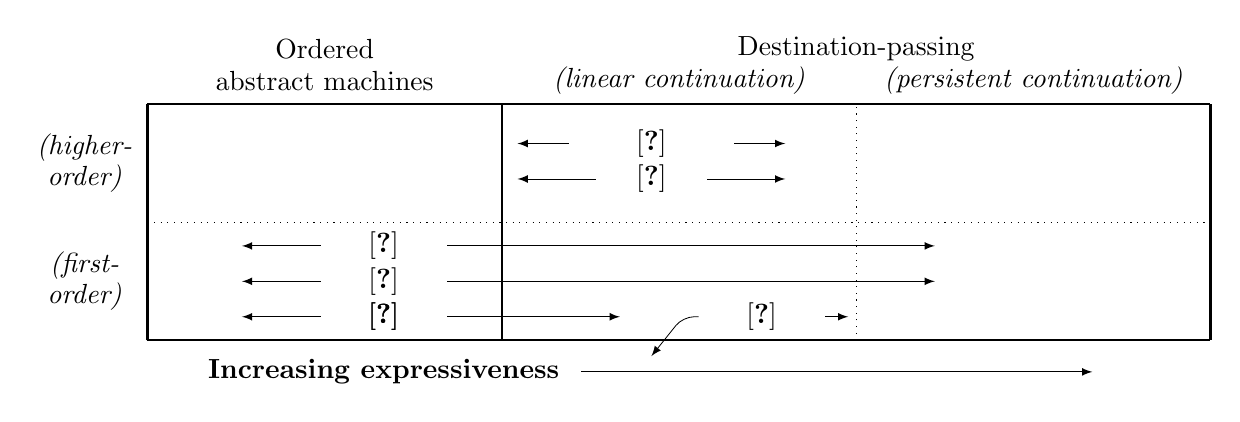
\begin{tikzpicture} 
\draw[thick](0cm,0cm) -- (0cm,3cm);
\draw (2.25,3.7) node{Ordered};
\draw (2.25,3.3) node{abstract machines};
%
\draw[thick](4.5cm,0cm) -- (4.5cm,3cm);
\draw (9,3.7) node{Destination-passing};
\draw (6.75,3.3) node{\it (linear continuation)};
%
\draw[dotted](9cm,0cm) -- (9cm,3cm);
\draw (11.25,3.3) node{\it (persistent continuation)};
%
\draw[thick](13.5cm,0cm) -- (13.5cm,3cm);
%
\draw[thick](0,0) -- (13.5,0);
\draw[dotted] (0,1.5) -- (13.5,1.5);
\draw[thick](0,3) -- (13.5,3);
%
\draw (-.8,2.45) node{\it (higher-};
\draw (-.8,2.05) node{\it order)};
%
\draw (-.8,0.95) node{\it (first-};
\draw (-.8,0.55) node{\it order)};
%
\draw (3,1.2) node{\cite{pfenning04substructural}};
\draw (3,.75) node{\cite{pfenning09substructural}};
\draw (3,.3) node{\cite{simmons11logical}};
\draw (3,.3) node{\cite{simmons11logical}};
\draw (7.8,.3) node{\cite{pfenning12substructural}};
\draw (6.4,2.5) node{\cite{cervesato02concurrent}};
\draw (6.4,2.05) node{\cite{schacknielsen07induction}};
\draw (3,-.4) node{\bf Increasing expressiveness};
%
\pgfsetarrowsstart{latex} 
\pgfsetlinewidth{.3pt} 
\pgfusepath{stroke} 
\draw (1.2,1.2) -- (2.2,1.2);
\draw (10,1.2) -- (3.8,1.2);
\draw (1.2,.75) -- (2.2,.75);
\draw (10,.75) -- (3.8,.75);
\draw (1.2,.3) -- (2.2,.3);
\draw (6,.3) -- (3.8,.3);
\draw[rounded corners=4pt] (6.4,-.2) -- (6.8,.3) -- (7,.3);
\draw (8.9,.3) -- (8.6,.3);
\draw (4.7,2.5) -- (5.35,2.5);
\draw (4.7,2.05) -- (5.7,2.05);
\draw (8.1,2.5) -- (7.45,2.5);
\draw (8.1,2.05) -- (7.1,2.05);
%
\draw (12,-.4) -- (5.5,-.4);
\end{tikzpicture} 
\end{center}
\caption{Classification of existing work on SSOS specifications.}
\label{fig:class-prevwork}
\end{figure}

This classification of substructural operational semantics is
illustrated graphically in Figure~\ref{fig:class-prevwork}. Existing
published work on substructural operational semantics specifications
is placed in the figure, with arrows indicating the range of styles
that are considered. With the possible exception of certain aspects of
the SSOS presentation in Pfenning's course notes
\cite{pfenning12substructural}, the taxonomy described above neatly
captures previous work. 

The statement that each specification style is strictly more
expressive than the last is formal: there are automatic and
provably-correct transformations from the expressive styles (natural
semantics and ordered abstract machines) to the more expressive
formalisms (ordered abstract machines and destination-passing).  The
investigation of provably-correct transformations on
\sls~specifications is therefore the means by which we classify of
SSOS semantics. We call this methodology the {\it logical
  correspondence}, and it is the focus of this portion of the thesis,
which justifies the following argument:

\begin{quote} 
  {\bf Thesis (part 2):} A logical framework based on forward
  reasoning in substructural logic supports many styles of programming
  language specification. These styles can be formally classified and
  connected by considering general transformations on logical
  specifications. 
 
  Generally applicable transformations on logical
  specifications are also useful for deriving manifestly correct
  program analyses from those operational semantics specifications.
\end{quote} 

\noindent
In this introductory chapter, we will outline our use of logical
correspondence and connect it to previous work. The development of the
logical correspondence as presented in this chapter, and the
operationalization and defunctionalization transformations presented
in the next chapter, represent joint work with Ian Zerny.

\section{Logical correspondence}

As stated above, we will primarily discuss and connect three different
styles that are used specifying the operational semantics of
programming languages. Natural semantics is a high-level, declarative
style of specification. For illustration, the call-by-value natural
semantics for the untyped lambda calculus is comprised of two rules:
\[
\infer[{\sf ev/lam}]
{\lambda x. e \Downarrow \lambda x. e \mathstrut}
{}
\quad
\infer[{\sf ev/app}]
{e_1\,e_2 \Downarrow v \mathstrut}
{e_1 \Downarrow \lambda x.e
 &
 e_2 \Downarrow v_2
 &
 [v_2/x]e \Downarrow v \mathstrut}
\]
This inductive definition assigns meaning to all the terminating
expressions in the lambda calculus. However, natural semantics are not
{\it operational} semantics, except in the very loose sense that they
are {\it moded} in the sense of Section~\ref{sec:framework-modes}: we
can think of the $e$ in $e \Downarrow v$ as being an input and the $v$
as being output. The order of evaluation is unspecified, however.  In
rule ${\sf ev/app}$, the subexpressions $e_1$ and $e_2$ can be
evaluated to values in either order and can even be evaluated in
parallel.

We turn natural semantics into ordered abstract machines by
a transformation called {\it operationalization}, and turn ordered
abstract machine specifications into destination-passing
specifications by a transformation called {\it destination-adding}.
Destination-passing specifications can then be transformed into a
collecting semantics by the simple transformation of {\it
  abstraction}, after which they can be further abstracted to obtain
program analyses like control flow analysis. These major
transformations are presented graphically in
Figure~\ref{fig:class-transform}.

\begin{figure}
\begin{center}
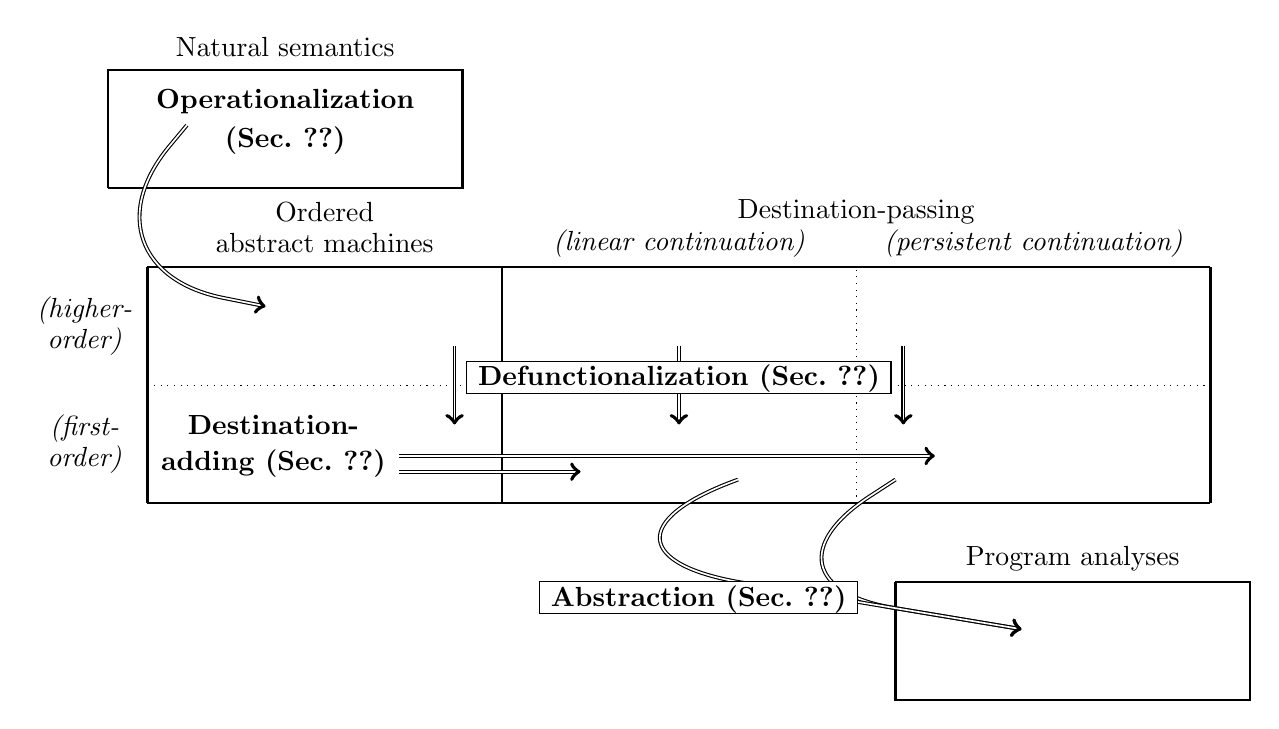
\begin{tikzpicture}
\draw (1.75,5.8) node{Natural semantics};
\draw[thick](-.5cm,4cm) -- (-.5cm,5.5cm) -- (4cm,5.5cm) 
  -- (4cm,4cm) -- (-.5cm,4cm);
%
\draw (11.75,-.7) node{Program analyses};
\draw[thick](9.5cm,-1cm) -- (9.5cm,-2.5cm) -- (14cm,-2.5cm) 
  -- (14cm,-1cm) -- (9.5cm,-1cm);
%
\draw[thick](0cm,0cm) -- (0cm,3cm);
\draw (2.25,3.7) node{Ordered};
\draw (2.25,3.3) node{abstract machines};
%
\draw[thick](4.5cm,0cm) -- (4.5cm,3cm);
\draw (9,3.7) node{Destination-passing};
\draw (6.75,3.3) node{\it (linear continuation)};
%
\draw[dotted](9cm,0cm) -- (9cm,3cm);
\draw (11.25,3.3) node{\it (persistent continuation)};
%
\draw[thick](13.5cm,0cm) -- (13.5cm,3cm);
%
\draw[thick](0,0) -- (13.5,0);
\draw[dotted] (0,1.5) -- (13.5,1.5);
\draw[thick](0,3) -- (13.5,3);
%
\draw (-.8,2.45) node{\it (higher-};
\draw (-.8,2.05) node{\it order)};
%
\draw (-.8,0.95) node{\it (first-};
\draw (-.8,0.55) node{\it order)};
%
\draw[double,->] (3.9,2) -- (3.9,1);
\draw[double,->] (6.75,2) -- (6.75,1);
\draw[double,->] (9.6,2) -- (9.6,1);
\draw (6.75,1.6) node {\fboxsep=0pt\fbox{\colorbox{white}{\rule[-0.5ex]{0em}{2.5ex}\bf ~Defunctionalization~(Sec.~\ref{sec:defunctionalization})~}}};
%
\draw (1.75,5.1) node {\bf Operationalization};
\draw (1.75,4.6) node {\bf (Sec.~\ref{sec:operationalization})~};
\draw[double,->,rounded corners=2cm] (.5,4.8) -- (-1,3) -- (1.5,2.5);
%
\draw (1.6,1) node {\bf Destination-};
\draw (1.6,.5) node {\bf adding (Sec.~\ref{sec:destination-adding})};
\draw[double,->] (3.2,.6) -- (10,.6);
\draw[double,->] (3.2,.4) -- (5.5,.4);
%
\draw[double,->,rounded corners=2cm] (9.5,.3) -- (7.5,-1) -- (11.1,-1.6);
\draw[double,->,rounded corners=2.5cm] (7.5,.3) -- (5.1,-.6) -- (11.1,-1.6);
\draw (7,-1.2) node {\fboxsep=0pt\fbox{\colorbox{white}{\rule[-0.5ex]{0em}{2.5ex}\bf ~Abstraction~(Sec.~\ref{sec:abstraction})~}}};
\end{tikzpicture} 
\end{center}
\caption{Major transformations on \sls~specifications.}
\label{fig:class-transform}
\end{figure}

There are many other smaller design decisions that can be made in the
creation of a substructural operational semantics. Only one is
graphically represented in
Figures~\ref{fig:class-prevwork}~and~\ref{fig:class-transform}, the
distinction between {\it higher-order} or {\it first-order}
specifications. This distinction applies to all concurrent
\sls~specifications, not just those that specify substructural
operational semantics. First-order
specifications are like rewriting rules $\left( p_1 \fuse \ldots \fuse
  p_n \lefti \{ q_1 \fuse \ldots \fuse q_m \} \right)$, where the head
of the rule $\{ q_1 \fuse \ldots \fuse q_m \}$ contains only atomic
propositions. Higher-order \sls~specifications, on the other hand,
contain {\it rules} in the conclusions of rules; when the rule fires,
the resulting process state contains the rule. An example is given 
in Figure~\ref{fig:ho-evo-ex}.
Order matters in higher-order process states: $\left(x{:}\susp{\sf p1(c)}, ~
y{:}\istrue{\left( {\sf p1(c)} \lefti \{ {\sf p2(c)} \} \right)}\right)
\leadsto \left(z{:}\susp{\sf p2(c)}\right)$, whereas 
$\left(y{:}\istrue{\left( {\sf p1(c)} \lefti \{ {\sf p2(c)} \} \right)},~
x{:}\susp{\sf p1(c)}\right)
\not \leadsto$. 
%
The choice of higher-order versus first-order specification does not
impact expressiveness, but it does influence our ability to read
specifications (opinions differ as to which style is clearer) and 
the ways we reason about them.

\begin{figure}
\begin{align*}
x_1{:}\susp{{\sf p2}({\sf c})}, ~~
x_2{:}\susp{{\sf p1}({\sf c})}, ~~
x_3{:}\istrue{(\forall x.\,{\sf p_1}(x) 
                \lefti \{ {\sf p_2}(x) \lefti \{ {\sf p_3}(x) \} \})}, ~~
x_4{:}\istrue{({\sf p3}({\sf c}) \lefti \{ {\sf p_4} \})} & \\
\leadsto ~~~ 
x_1{:}\susp{{\sf p2}({\sf c})}, ~~
x_5{:}\istrue{({\sf p_2}({\sf c}) \lefti \{ {\sf p_3}({\sf c}) \})}, ~~
x_4{:}\istrue{({\sf p3}({\sf c}) \lefti \{ {\sf p_4} \})} & \\
\leadsto ~~~ 
x_6{:}\susp{{\sf p3}({\sf c})}, ~~
x_4{:}\istrue{({\sf p3}({\sf c}) \lefti \{ {\sf p_4} \})} & \\
\leadsto ~~~ 
x_7{:}\susp{{\sf p_4}} & 
\end{align*}
\caption{Evolution of a higher-order \sls~process state (${\sf p1}$, ${\sf
  p2}$ and ${\sf p3}$ are all ordered atomic propositions).}
\label{fig:ho-evo-ex}
\end{figure}

Other distinctions between \sls~specifications can also be understood
in terms of nondeterministic choices that can be made by the various
transformations we consider: for instance, the operationalization
transformation can produce ordered abstract machines that evaluate
subcomputations in parallel or in sequence or not, and the
destination-adding transformation can make continuations either linear
or persistent. The existence of these nondeterministic choices have two
important consequences. First, it is generally the case that one source
specification (a natural semantics or an ordered abstract machine
specification) can give rise to several different target
specifications (ordered abstract machine specifications or
destination-passing specifications). The correctness of the
transformation also acts as a simple proof of the equivalence of the
several target specifications.

The other interesting consequence of nondeterministic choices is the
different options give us a rigorous vocabulary for describing choices
that otherwise seem ad-hoc. An example of this can be found in the
paper that introduced the destination-adding and abstraction
transformations \cite{simmons11logical}. In that article, we had to
motivate an ad-hoc change to the usual abstract machine semantics. In
this thesis, by the time we encounter a similar specification in
Chapter 8, we will be able to see that this distinction corresponds to
the choice of whether or not tail-recursion optimization is performed
during proof search.

\section{Related work}

This part of the thesis document document draws from many different
sources of inspiration. In this section, we survey this related work
and, where applicable, outline how our use of logical correspondence
differs from existing work.

\subsection{Partiality in deductive computation}

The genesis of the operationalization transformation discussed in
Chapter~6 can be found in the treatment of the operational semantics
of LF in Tom Murphy VII's thesis \cite{murphy08modal}. In his thesis,
Murphy described a natural semantics for Lambda 5, a distributed
programming language, and then wanted to interpret that natural
semantics as an {\it operational} semantics for Lambda 5. As discussed
above, natural semantics are not operational. However, by interpreting
the natural semantics as a moded logic program, Murphy stipulated that
the operational semantics were precisely those given by moded, {\it
  non-backtracking} deductive proof search. Then, by modifying the
checks that Twelf performs with a special purpose partiality
directive, he was able to check that moded proof search would never
fail and never backtrack, though it might diverge. This check amounted
to a proof of safety (progress and preservation) for his natural
semantics. I believe his mechanized proof to be the only existing
non-classical proof of safety for a big-step operational semantics.

Murphy's proof only works because his formulation of Lambda 5 was {\it
  intrinsically typed}, meaning that, using the facilities provided by
LF's dependent types, he enforced that only well-typed terms could
possibly be evaluated. His approach would also work for our untyped
lambda calculus above, as closed terms in the untyped lambda calculus
can never get stuck. However, as soon as we extend the untyped lambda
calculus with some other values (numbers, Booleans, pairs, etc\ldots)
or even just with a nonsense term ${\sf junk}$, then progress and
preservation apply only to well-typed and not to arbitrary terms. In
this case, Murphy's partiality checks no longer hold, so we cannot use
his methodology to reason about safety. 

One way to look at the operationalization transformation presented in
Chapter~6 is as a way to make the internal structure of a deductive
computation explicit as a concurrent computation. Having done so, we
can explicitly represent complete, unfinished, and stuck (or failing)
computations as concurrent traces and reason about these traces with a
richer set of tools than the limited set Murphy successfully utilized.

\subsection{A coinductive interpretation}

Murphy proved safety for a natural semantics specification by
reinterpreting the inductive definition of the natural semantics as a
logic program and reasoning about the logic program. Leroy and Grall,
in \cite{leroy09coinductive}, use a different reinterpretation: they
reinterpret the inductive definition of natural semantics as 
a {\it coinductive} specification, that is, the {\it greatest} fixed point
of the following rules.
\[
\infer%[{\sf evco/lam}]
{\lambda x. e \Downarrow^{\sf co} \lambda x. e \mathstrut}
{}
\quad
\infer%[{\sf evco/app}]
{e_1\,e_2 \Downarrow^{\sf co} v \mathstrut}
{e_1 \Downarrow^{\sf co} \lambda x.e
 &
 e_2 \Downarrow^{\sf co} v_2
 &
 [v_2/x]e \Downarrow^{\sf co} v \mathstrut}
\]
Of course, aside from the ${\sf co}$ annotation and the different
interpretation, these rules are syntactically identical to the inductively
defined natural semantics above.

Directly reinterpreting the inductive specification as an inductive
specification doesn't quite produce the right result: for some
diverging terms like $\omega = (\lambda x.\,x\,x)\,(\lambda
x.\,x\,x)$, we can derive $\omega \Downarrow^{\sf co} e$ for any
expression $e$, including expressions that are not values and
expressions like ${\sf junk}$ with no relation to the original
term. Conversely, there are diverging terms ${\it Div}$ such that
${\sf div} \Downarrow^{\sf co} e$ is not derivable for {\it any}
$e$.\footnote{Leroy and Grall discuss a counterexample due to Filinski
  where ${\it Div} = {\it Y}{\it F}x$ where $\it Y$ is the fixed-point
  combinator $\lambda f.\,(\lambda x.\,f\,(\lambda
  v.\,(x\,x)\,v))\,(\lambda x.\,f\,(\lambda v.\,(x\,x)\,v))$ and $\it
  F$ is $\lambda f.\,\lambda x.\,(\lambda g.\,\lambda
  y.\,g\,y)\,(f\,x)$ \cite{leroy09coinductive}.} As a result, Leroy
and Grall also give a greatest-fixed-point definition of diverging
terms $e \Downarrow^\infty$ that is based on the least-fixed-point
specification $e \Downarrow v$.
\[
\infer%[{\sf div/app1}]
{e_1\,e_2 \Downarrow^\infty}
{e_1 \Downarrow^\infty}
\quad
\infer%[{\sf div/app2}]
{e_1\,e_2 \Downarrow^\infty}
{e_1 \Downarrow (\lambda x.\,e)
 & 
 e_2 \Downarrow^\infty}
\quad
\infer%[{\sf div/app3}]
{e_1\,e_2 \Downarrow^\infty}
{e_1 \Downarrow (\lambda x.\,e)
 & 
 e_2 \Downarrow v_2
 &
 [v_2/x]e \Downarrow^\infty}
\]
Now diverging expressions are fully characterized as derivations for
which $e \Downarrow^\infty$ is derivable by infinite derivation trees,
thereby capturing both converging and diverging executions.  With this
definition, Leroy and Grall prove a type safety property: if $e$ has
type $\tau$, then either $e \Downarrow v$ or $e \Downarrow^{\infty}$.
However, the disjunctive character of this theorem means that a
constructive proof of type safety would be required to take a typing
derivation $e : \tau$ as input and produce as output either a proof of
termination $e \Downarrow v$ or a proof of divergence $e
\Downarrow^\infty$. This seems to imply that a constructive type
safety theorem would additionally decide termination, and so it is
unsurprising that type safety is proved classically by Leroy and Grall.

We suggest that the operationalization transformation, seen as a
logical extension to Murphy's methodology, is superior to the
coinductive (re)interpretation as a way of understanding the behavior
of infinite terms in the natural semantics. Both approaches
reinterpret the logical artifact of natural semantics in an
operational way, but the operationalization transformation gives us a
satisfactory treatment of diverging terms without requiring the
definition of an additional coinductive judgment $e
\Downarrow^\infty$.

\subsection{The functional correspondence}

The ordered abstract machine that results from our operationalization
transformation corresponds to a standard abstract machine model (a
statement we will make precise in
Section~\ref{sec:nat-ssos-adequacy}). In this sense, the logical
correspondence has a great deal in common with the {\it functional
  correspondence} of Ager, Danvy, Midtgaard, and
others~\cite{ager03functional,ager04functional,ager05functional,
  danvy08defunctionalized,danvy12interderiving}. 

The goal of the functional correspondence is encode various styles of
semantic specifications (natural semantics, abstract machines,
small-step structural operational semantics, environment semantics,
etc.) as functional programs. It is then possible to show that these
styles can be related by off-the-shelf and fully correct
transformations on functional programs. The largest essential difference
between the functional and logical correspondences, then, is that
the functional correspondence acts on functional programs, whereas
the logical correspondence acts on specifications encoded in a logical
framework (in our case, the logical framework \sls). 

While the functional and logical correspondences can be 


However, the functional correspondence as given assumes that 
semantic specifications are adequately represented as functional
programs. 
%
The
%interpretations
representations and the adequacy of the encoding with respect to the ``on paper''
semantics is an assumed prerequisite in existing work. 
% tighten this next sentence up
This is potentially
problematic: the function space of a general programming language
is much more open-ended than necessary or even desirable. The correspondence
remains a useful methodology, but is not 
directly applicable to the analysis 
(particularly mechanized analysis) of semantic specifications.


\subsection{Transformation on specifications}

 This aspect of
operationalization -- taking a logical specification of a language's
natural semantics and transforming it to obtain an abstract machine --
has been explored by others, including Hannan and Miller
\cite{hannan92operational} and Ager \cite{ager04natural} have also
proposed the idea of operationalizing natural semantics specifications
as abstract machines by provably correct and general transformations
on logical specifications (in the case of Hannan and Miller) or on the
special-purpose framework of L-attributed natural semantics (in the
case of Ager). 

A major difference in this case is that both lines of
work result in {\it deductive} specifications of abstract
machines. Our translation into concurrent specifications has the
advantage of exploiting parallelism, as demonstrated in
Section~\ref{sec:trans-par} below, and also opens up specifications to
the modular inclusion of stateful and concurrent features, as we will
discuss in Section~\ref{sec:richer-ordered-abstract}.


\section{Expressiveness and modular extension}

Much of the work in the previous section concerned itself with {\it
  correspondence} -- in both the work of Ager et al.~and the work of
Hannan and Miller, two or more specifications (often natural semantics
and abstract machines) are presented and then shown to correspond
exactly. But it is not my intent to advocate strongly for the use of
natural semantics specifications; recall that natural semantics were
used to illustrate problems with {\it non}-modularity in language
specification in Section~\ref{sec:modularnonmodular}. Instead, our
use 

The functional correspondence is largely concerned with the 

\sls~is very
The potential design space of substructural operational semantics is
quite large. 

I propose that different styles of
\sls~specification can be productively classified in terms of the
transformations that turn one classification style into another. Most
transformations will not have inverses, so this methodology gives us a
formal notion of which styles are more expressive than others.
Considering logical transformations also can lower the cost of
mis-prediction. If one begins a development in an overly-restrictive
style, the development can be transformed into a more expressive style
by an automatic transformation.






% Ordered abstract machines
\chapter{Ordered abstract machines}
\label{chapter-absmachine}

This chapter centers around two transformations on logical
specifications.  Taken together, the operationalization transformation
(Section~\ref{sec:operationalization}), and the defunctionalization
transformation (Section~\ref{sec:defunctionalization}) allow us to
establish the logical correspondence between the deductive SLS
specification of a natural semantics and the concurrent SLS
specification of an abstract machine.

Natural semantics specifications are common in the literature,
and are also easy to encode in either the deductive fragment of
\sls~or in a purely deductive logical framework like LF.  We will
continue to use the natural semantics specification of call-by-value
evaluation for the lambda calculus as a running example:
\[
\infer[{\sf ev/lam}]
{\lambda x. e \Downarrow \lambda x. e \mathstrut}
{}
\quad
\infer[{\sf ev/app}]
{e_1\,e_2 \Downarrow v \mathstrut}
{e_1 \Downarrow \lambda x.e
 &
 e_2 \Downarrow v_2
 &
 [v_2/x]e \Downarrow v \mathstrut}
\]

Abstract machine semantics are less prevalent than natural
semantics. The most well-known is almost certainly Landin's SECD
machine \cite{landin64mechanical}, though our abstract machine
presentation is much more similar to Danvy's SC machine from
\cite{danvy03rational} and Harper's $\mathcal K\{{\sf
  nat}{\rightharpoonup}\}$ system from \cite[Chapter
27]{harper12practical}.  This abstract machine semantics is defined in
terms of states $s$. The state $s = k \rhd e$ represents the
expression $e$ being evaluated on top of the stack $k$, and the state
$s = k \lhd v$ represents the value $v$ being returned to the stack
$k$. Stacks $k$ are sequences of frames $f_i$ with the form
$((\ldots({\sf halt}; f_1); \ldots); f_n)$, and each frame $f$ either
has the form $\Box\,e_2$ (an application frame waiting for an
evaluated function to be returned to it) or the form $(\lambda
x.e)\,\Box$ (an application frame with an evaluated function waiting
for an evaluated value to be returned to it). Given states, stacks,
and frames, we can define a ``classical'' abstract machine for
call-by-value evaluation of the lambda calculus as a transition system
with four transition rules:
\begin{align*}
{\sf absmachine/lam}{:} & ~~ k \rhd \lambda x.e ~ \mapsto ~ k \lhd \lambda x.e
\\
{\sf absmachine/app}{:} & ~~ k \rhd e_1\,e_2 ~ \mapsto ~ (k; \Box\,e_2) \rhd e_1
\\
{\sf absmachine/app1}{:} & ~~ 
  (k; \Box\,e_2) \lhd \lambda x.e ~ \mapsto ~ (k; (\lambda x.e)\,\Box) \rhd e_2
\\
{\sf absmachine/app2}{:} & ~~
  (k; (\lambda x.e)\,\Box) \lhd v_2 ~ \mapsto ~ k \rhd [v_2/x]e
\end{align*}

The operational intuition for these rules is precisely the same as the
operational intuition for the rewriting rules given in
Section~\ref{sec:intro-ssos}. This is not coincidental: the
\sls~specification from the introduction adequately encodes the
transition system $s \mapsto s'$ defined above, a point that we will
make precise in Section~\ref{sec:nat-ssos-adequacy}. The
\sls~specification from the introduction is {\it also} the result of
applying the operationalization and defunctionalization
transformations to the \sls~encoding of the natural semantics given
above, so the these two transformations combined with the adequacy
arguments at either end constitute a logical correspondence between
natural semantics and abstract machines. 

As discussed in Section~\ref{sec:the-point-is-modular-extension}, it
is interesting to put existing specification styles into logical
correspondence, but that is not our main reason for investigating
logical correspondence. Instead, we are primarily interested in
exploring the set of programming language features that can be
modularly integrated into a transformed \sls~specification that could
not be integrated into a natural semantics specification.  In
Section~\ref{sec:richer-ordered-abstract} we explore a selection of
these features, including mutable storage, call-by-need evaluation,
and recoverable failure.

\section{Logical transformation: operationalization}
\label{sec:operationalization}

The intuition behind operationalization is rather simple: we examine
the behavior of a deductive computation and then encode that
operational intuition as a concurrent computation.  Before presenting
the general transformation, we will motivate this transformation using
our natural semantics specification of call-by-value-evaluation. 

The definition of $e \Downarrow v$ is moded with $e$ as an input and
$v$ as an output, so it is meaningful to talk about being given $e$
and using deductive computation to search for a $v$ such that $e
\Downarrow v$ is derivable.  Consider a recursive search procedure
implementing this particular deductive computation:
\begin{itemize}
\item
      If $e = \lambda x. e'$, 
      it is possible to derive 
      $\lambda x. e' \Downarrow \lambda x. e'$
      with the rule ${\sf ev/lam}$.
\item
       If $e = e_1\,e_2$,
       attempt to derive 
       $e_1\,e_2 \Downarrow v$
       using the rule ${\sf ev/app}$ by doing the following:
    \begin{enumerate}
    \item Search for a $v_1$ such that 
          $e_1 \Downarrow v_1$ is derivable.
    \item Assert that $v_1 = \lambda x.e'$ for some
          $e'$; fail if it is not.
    \item Search for a $v_2$ such that 
          $e_2 \Downarrow v_2$ is derivable.
    \item Search for a $v$ such that 
          $[v_2/x]e \Downarrow v$ is derivable.
    \end{enumerate}
% \item
%       If $e = e_1 \arb e_2$,
%       attempt to derive $e_1 \arb e_2 \Downarrow v$ using
%       the rule ${\sf ev/choose1}$ by searching for a 
%       $v$ such that $e_1 \Downarrow v$ is derivable.
% \item
%       If $e = e_1 \arb e_2$,
%       attempt to derive $e_1 \arb e_2 \Downarrow v$ using 
%       the rule ${\sf ev/choose2}$ by searching for a 
%       $v$ such that $e_2 \Downarrow v$ is derivable.  
\end{itemize}
%
The goal of the operationalization transformation is to implement this
deductive computation as a concurrent computation. The first step in
doing so is to introduce two new ordered atomic propositions.  The
proposition ${\sf eval}\,\interp{e}$ is the starting point, indicating
that we want to search for a $v$ such that $e \Downarrow v$, and the
proposition ${\sf retn}\,\interp{v}$ indicates the successful
completion of this procedure. Therefore, searching for a $v$ such that
$e \Downarrow v$ is derivable will be analogous to building a trace $T
:: x_e{:}\susp{{\sf eval}\,\interp{e}} \leadsto^* x_v{:}\susp{{\sf
    retn}\,\interp{v}}$ with concurrent computation.

Representing the first case is straightforward: if we are evaluating
$\lambda x.e$, then we have succeeded and can return $\lambda x.e$. 
This is encoded as the following proposition:
\[
{\sf eval}\,({\sf lam}\,\lambda x.\,E\,x)
   \lefti \{ {\sf retn}\,({\sf lam}\,\lambda x.\,E\,x) \}
\]
Because the natural deduction rule ${\sf ev/app}$ 
involves both recursion and multiple subgoals,
we will generalize our picture of the process state to allow us to store a
stack of unfinished work in the ordered context, growing out to the
right. Our new understanding, then, is that contexts either have the
form $x{:}\susp{{\sf eval}\,\interp{e}}, \Delta$ or the form $x{:}\susp{{\sf
  retn}\,\interp{v}}, \Delta$. In the process of concurrently
computing a trace $x_e{:}\susp{{\sf eval}\,\interp{e_1\,e_2}}, \Delta
\leadsto^* x_v{:}\susp{{\sf retn}\,\interp{v}}, \Delta$, each of the
recursive calls to the search procedure will involve a sub-trace of the
form
%
\[x_e{:}\susp{{\sf eval}\,\interp{e'}}, y{:}\istrue{A^-}, \Delta
  \leadsto^*
  x_v{:}\susp{{\sf retn}\,\interp{v'}}, y{:}\istrue{A^-}, \Delta\]
%
  where $A^-$ is a negative proposition that is prepared to interact
  with the subgoal's final ${\sf retn}\,\interp{v'}$ proposition to
  kickstart the rest of the computation.

It's helpful to work backwards: in the fourth step, we have found
$\lambda x.\,E\,x = \lambda x.\interp{e}$ (where $e$ potentially has $x$ free) and $V_2 =
\interp{v_2}$. The recursive call is to ${\sf
  eval}\,\interp{[v_2/x]e}$, which is the same thing as ${\sf
  eval}\,(E\,V_2)$. If the recursive call successfully returns, the
context will contain a suspended atomic proposition of the form ${\sf
  retn}\,V$ where $V = \interp{v}$, and the search procedure as a
whole is complete: the answer is $v$.  Thus, the negative proposition
that implements the continuation can be written as $(\forall V.\,{\sf
  retn}\,V \lefti \{ {\sf retn}\,V \})$. The positive proposition that
will create this sub-computation can be written as follows:
\begin{align*}
{\it Step_4}(E,V_2) & \equiv {\sf eval}\,(E\,V_2) 
\fuse {\downarrow}(\forall V.\, {\sf retn}\,V \lefti \{ {\sf retn}\,V \})
%
\intertext{Moving backwards, in the third step we have a $E_2 =
  \interp{e_2}$ that we were given and $\lambda x.\,E\,x = \lambda x.\interp{e}$ that we
  have computed. The recursive call is to ${\sf
    eval}\,\interp{e_2}$, and assuming that it completes, we need
  to begin the fourth step. The positive proposition that will 
  create this sub-computation can be written as follows:}
%
{\it Step_3}(E_2,E) & \equiv {\sf eval}\,E_2 
\fuse {\downarrow}(\forall V_2.\,
  {\sf retn}\,V_2 \lefti \{ {\it Step_4}(E,V_2) \})
%
\intertext{Finally, the first two steps can be handled together. We have
$E_1 = \interp{e_1}$ and $E_2 = \interp{e_2}$; the recursive
call is to ${\sf eval}\,\interp{e_1}$. Once the
recursive call completes, we can enforce that the returned value has
the form $\interp{\lambda x.e}$ before proceeding
to the continuation.}
{\it Step_{1,2}}(E_1, E_2) & \equiv {\sf eval}\,E_1
\fuse {\downarrow}(\forall E.\, {\sf retn}\,({\sf lam}\,\lambda x.\,E\,x)
\lefti \{ {\it Step_3}(E_2, E)\})
\end{align*}
Thus, the rule implementing this entire portion of the search
procedure is 
\[
\forall E_1.\,\forall E_2.\,
{\sf eval}\,({\sf app}\,E_1\,E_2) \lefti \{ {\it
  Step_{1,2}}(E_1, E_2) \}
\]
The \sls~encoding of our example natural semantics is shown in
Figure~\ref{fig:example-transform-cbv} alongside the transformed
specification, which has the form of an ordered abstract machine
semantics, though it is different than the ordered abstract machine
semantics presented in the introduction. We say the specification
above is {\it higher-order}, as ${\sf ev/app}$ is a rule that, when it
participates in a transition, produces a new rule $(\forall E.\,{\sf
  retn}\,({\sf lam}\,\lambda x.\,E\,x) \lefti \{ \ldots \})$ that
lives in the context. (In contrast, the ordered abstract machine
semantics from the introduction was {\it first-order}.)  We discuss
the defunctionalization transformation, which allows us to derive
first-order specifications from specifications that are higher-order
in this way, in Section~\ref{sec:defunctionalization} below.

\begin{figure}
\begin{minipage}[b]{0.36\linewidth}
\fvset{fontsize=\small,boxwidth=auto}
\VerbatimInput{sls/cbv-ev.sls}
\end{minipage}
\hspace{0.5cm}
\begin{minipage}[b]{0.64\linewidth}
\fvset{fontsize=\small,boxwidth=auto}
\VerbatimInput{sls/cbv-ev-ssos.sls}
\end{minipage}
\caption{A natural semantics for CBV (left) and the corresponding (higher-order)
  ordered abstract machine (right).}
\label{fig:example-transform-cbv}
\end{figure}

The intuitive connection between natural semantics specifications and
concurrent specifications has been explored previously and
independently in the context of CLF by Schack-Nielsen
\cite{schacknielsen07induction} and by Cruz and Hou
\cite{cruz12parallel}; Schack-Nielsen proves the equivalence of the
two specifications, whereas Cruz and Favonia used the connection
informally. The contribution of this section is to describe a general
transformation (of which Figure~\ref{fig:example-transform-cbv} is one
instance) and to prove the transformation correct in general. I have
implemented the operationalization transformation within my prototype
typechecker for \sls~specifications, whereas the defunctionalization 
transformation is not implemented and will be treated somewhat more
informally.

In Section~\ref{sec:trans-subset} we will present the subset of
specifications that our operationalization transformation handles, and
in Section~\ref{sec:trans-basic} we present the most basic form of the
transformation.  In
Sections~\ref{sec:trans-tail}~and~\ref{sec:trans-par} we extend the
basic transformation to be both tail-recursion optimizing and
parallelism-enabling. Finally, in
Section~\ref{sec:operationalization-correct}, we establish the
correctness of the overall transformation.

\subsection{Transformable signatures}
\label{sec:trans-subset}

The starting point for the operationalization transformation is a
deductive signature that is well-moded in the sense described in
Section~\ref{sec:framework-modes}. Every declared negative predicate
will either remain defined by deductive proofs (we write these
predicates as ${\sf ad}$ and write the atomic propositions built with
these predicates as $p_d^-$, $d$ for deductive) or will be transformed
so that it is concurrently defined (we write these predicates as ${\sf
  ac}$ and write the atomic propositions built with these predicates
as $p_c^-$, $c$ for concurrent).

For the purposes of describing and proving the correctness of the
operationalization transformation, we will assume that all transformed
atomic propositions $p_c^-$ have two arguments where the first
argument is moded as an input and the second is an output. That is,
they are declared as follows:
\begin{align*}
& {\sf \#mode~a~{+}~{-}}.\\
& {\sf ac} : \tau_1 \rightarrow \tau_2 \rightarrow {\sf prop}.
\end{align*}
Without dependency, two-place relations are sufficient for describing
$n$-place relations.\footnote{As an example, to handle addition on
  natural numbers, defined as a three-place relation ${\sf add} : {\sf
    nat} \rightarrow {\sf nat} \rightarrow {\sf nat} \rightarrow {\sf
    type}$ with its usual mode (${\sf add}~{+}~{+}~{-}$), we define a
  unique type ${\sf add\_in}$ with one binary constructor ${\sf
    add\_c} : {\sf nat} \rightarrow {\sf nat} \rightarrow {\sf
    add\_in}$. Then we can declare (${\sf add'} : {\sf add\_in}
  \rightarrow {\sf nat} \rightarrow {\sf type}$) with mode (${\sf
    add'}~{+}~{-}$).}  It should be possible to handle dependent
predicates (that is, those with declarations of the form ${\sf ac} :
\Pi x{:}\tau_1.\,\tau_2(x) \rightarrow {\sf type}$), but we will not do
so here.

The restriction on signatures furthermore enforces that all rules must
be of the form ${\sf r} : C$ or ${\sf r} : D$, where $C$ and $D$ are
refinements of the negative propositions of \sls~that are defined as
follows:
\begin{align*}
C & ::= p^-_{c} 
    \mid \forall x{:}\tau.\, C
    \mid p^+_\mpers \lefti C
    \mid {!}p^-_c \lefti C
    \mid {!}G \lefti C \\
D & ::= p^-_{d}
    \mid \forall x{:}\tau.\, D
    \mid p^+_\mpers \lefti D
    \mid {!}p^-_c \lefti D
    \mid {!}G \lefti C \\
G & ::= p^-_d 
    \mid \forall x{:}\tau.\, G
    \mid p^+_\mpers \lefti G
    \mid {!}D \lefti G
\end{align*}
If {\it all} propositions are to remain deductive, then the
propositions $p^-_c$ and $C$ are irrelevant, and this restriction
describes all persistent, deductive specifications -- essentially, any
signature that could be executed by the standard logic programming
interpretation of LF \cite{pfenning89elf}. On the other hand, if all
propositions are to be transformed, then the propositions $p^-_d$ and
$D$ are irrelevant and this restriction amounts to restricting
rules to the Horn fragment.

All propositions $C$ are equivalent (at the level of synthetic
inference rules) to propositions of the form $\forall
\overline{x_0}\ldots \forall \overline{x_n}.\,A^+_n \lefti \ldots
\lefti A^+_1 \lefti {\sf ac}\,t_{0}\,t_{n+1}$, where the $\forall
\overline{x_i}$ are shorthand for a series of universal quantifiers
$\forall {x_{i1}}{:}{\tau_{i1}} \ldots \forall {x_{\it
    ik}}{:}{\tau_{\it ik}}$ and where each variable in
$\overline{x_i}$ does not appear in $t_0$ (unless $i = 0$) nor in any
$A^+_j$ with $j < i$ but does appear in $A^+_i$ (or $t_0$ if $i =
0$). Therefore, when we consider moded proof search, the variables
bound in $\overline{x_0}$ are all fixed by the query and those bound
in the other $\overline{x_i}$ are all fixed by the output position of
the $i^{\rm th}$ premise.

\subsection{Basic transformation}
\label{sec:trans-basic}

The operationalization transformation $\transop{\Sigma}$
operates on SLS signatures $\Sigma$ that have the form described in the
previous section. We
will first give the transformation on signatures; the transformation
of rule declarations ${\sf r} : C$ is the key case.

Each two-place predicate ${\sf ac}$ gets turned into two one-place
predicates ${\sf eval\_a}$ and ${\sf retn\_a}$: both ${\sf
  eval\_a}\,t$ and ${\sf retn\_a}\,t$ are positive ordered atomic
propositions.  We will write $\opsubst{X}$ for the operation of
substituting all occurrences of $p^-_c = {\sf ac}\,t_1\,t_2$ with
$({\sf eval\_a}\,t_1 \lefti \{ {\sf retn\_a}\,t_2 \})$ in $X$. This
substitution operation is used on propositions, contexts, and frames;
it appears in the transformation of rules ${\sf r} : D$ below.

\begin{itemize}
\item $\transop{\cdot} = \cdot$
\item $\transop{\Sigma, {\sf ac} : \tau_1 \rightarrow \tau_2
    \rightarrow {\sf prop}} = \transop{\Sigma}, ~ {\sf eval\_a} :
  \tau_1 \rightarrow {\sf prop\,ord}, ~ {\sf retn\_a} : \tau_2
  \rightarrow {\sf prop\,ord}$ 
\item $\transop{\Sigma, {\sf b} : K} = \transop{\Sigma}, ~ {\sf b}
  : K$ {\it (if ${\sf b} \neq {\sf ac}$)}
\item $\transop{\Sigma, {\sf c} : \tau} = \transop{\Sigma}, ~ {\sf
    c} : \tau$ 
\item $\transop{\Sigma, {\sf r} : C} = \transop{\Sigma}, ~ {\sf r}
  : \forall \overline{x_0}.\, {\sf eval\_a}\,t_0 \lefti \llbracket A^+_1,
  \ldots, A^+_n \rrbracket (t_{n+1}, {\sf id})$ \\ {\it (where $C$ is
    equivalent to $\forall \overline{x_0}\ldots \forall
    \overline{x_n}.\, A^+_n \lefti \ldots \lefti A^+_1 \lefti {\sf
      ac}\,t_{0}\,t_{n+1}$)}
\item $\transop{\Sigma, {\sf r} : D} = \transop{\Sigma}, ~ {\sf r}
  : \opsubst{D}$
\end{itemize}

The transformation of a proposition $C = \forall
\overline{x_0}\ldots \forall \overline{x_n}.\,A^+_n \lefti \ldots
\lefti A^+_1 \lefti {\sf ac}\,t_{0}\,t_{n+1}$ involves the definition
$\opbasic{A^+_i,\ldots,A^+_n}{t_{n+1}}{\sigma}$, where $\sigma$
substitutes only for variables in $\overline{x_j}$ where $j < i$. The
function is defined inductively on the length of the sequence
$A^+_i,\ldots,A^+_n$.

\begin{itemize}
\item $\opbasic{}{t_{n+1}}{\sigma} = \{ {\sf retn\_a}\,(\sigma{t_{n+1}}) \}$
\item $\opbasic{p^+_\mpers,A^+_{i+1},\ldots,A^+_n}{t_{n+1}}{\sigma} 
  = \forall \overline{x_i}.\, (\sigma{p^+_\mpers}) \lefti \opbasic{A^+_{i+1},\ldots,A^+_n}{t_{n+1}}{\sigma}$
\item $\opbasic{{!}p^-_c,A^+_{i+1},\ldots,A^+_n}{t_{n+1}}{\sigma}$
  \\
  $~ \qquad = \{ {\sf eval\_b}\,({\sigma}t^{\it in}_i) \fuse
  (\forall\overline{x_i}.\, {\sf retn\_b}\,(\sigma{t^{\it out}_i})
  \lefti \opbasic{A^+_{i+1},\ldots,A^+_n}{t_{n+1}}{\sigma}) \}$\\
  {\it (where $p^-_c$ is ${\sf bc}\,t^{\it in}_i\,t^{\it out}_i$)}
\item $\opbasic{{!}G,A^+_{i+1},\ldots,A^+_n}{t_{n+1}}{\sigma} = \forall
  \overline{x_i}.\, {!}(\sigma\opsubst{G}) \lefti
  \opbasic{A^+_{i+1},\ldots,A^+_n}{t_{n+1}}{\sigma}$
\end{itemize}

\noindent
This operation is slightly more general than it needs to be to
describe the transformation on signatures, where the substitution
$\sigma$ will always just be the identity substitution ${\sf id}$.
Non-identity substitutions arise during the proof of correctness, which
is why we introduce them here.

We have already given an example of the this basic operationalization
transformation, as Figure~\ref{fig:example-transform-cbv} is an
instance of this transformation.

\subsection{Tail-recursion}
\label{sec:trans-tail}

Consider again our motivating example, the procedure for that takes
expressions $e$ and searches for expressions $v$ such that $e
\Downarrow v$ is derivable. If we were to implement that procedure as
a functional program, the procedure would be {\it tail-recursive}. In
the procedure that handles the case when $e = e_1\,e_2$, the last step
is that the search procedure is invoked recursively. If and when that
callee returns $v$, then the caller will also return $v$.

Tail-recursion is significant in functional programming because
tail-recursive calls can be implemented without allocating a stack
frame: when a compiler makes this more efficient choice, we say it is
performing {\it tail-recursion optimization}.\footnote{Or {\it tail-call optimization}, as a tail-recursive function call is just a
  specific instance of a tail call.} An analogous opportunity for
tail-recursion optimization also arises in our logical compilation
procedure. In our motivating example, the last step in the $e_1\,e_2$
case was operationlized as a positive proposition of the form ${\sf
  eval}\,(E\, V) \fuse (\forall v.\,{\sf retn}\,v \lefti \{ {\sf
  retn}\,v \})$. In a successful search, the process state 
\[ x{:}{\sf
  eval}\,(E\, V), y{:}\istrue{(\forall v.\,{\sf retn}\,v \lefti \{
  {\sf retn}\,v \})}, \Delta\]
will concurrently compute until the
state 
\[ x'{:}{\sf retn}\,V, y{:}\istrue{(\forall v.\,{\sf retn}\,v \lefti
  \{ {\sf retn}\,v \})}, \Delta\] is reached, at which point the next
step \[y'{:}{\sf retn}\,V, \Delta\] is reached in one step by focusing
on $y$. 

If we operationalize the last step in the $e_1\,e_2$ case as ${\sf
  eval}\,(E\,V)$ instead of as ${\sf eval}\,(E\, V) \fuse (\forall
v.\,{\sf retn}\,v \lefti \{ {\sf retn}\,v \})$, we will reach the same
final state with one less transition. The tail-recursion optimizing
version of the operationalization transformation creates concurrent
computations that avoid these useless steps.

We cannot perform tail recursion in general because the output of the
last subgoal may be different from the output of the goal. For example,
the rule ${\sf r} : \forall{x}.\,\forall{y}.\,{!}{\sf a}\,x\,y \lefti
{\sf a}\,({\sf c}\,x)\,({\sf c}\,y)$ will translate to
\[ {\sf r} : \forall{x}.\,{\sf eval\_a}\,({\sf c}\,x) \lefti \{ {\sf
  eval\_a}\,x \fuse (\forall y.\, {\sf retn\_a}\,y \lefti \{ {\sf
  retn\_a}\,({\sf c}\,y) \} ) \} \] There is no opportunity for
tail-recursion optimization, because the output of the last search
procedure, $t^{\it out}_n = y$, is different than the value returned
down the stack, $t_{n+1} = {\sf c}\,y$. This case corresponds to
functional programs that cannot be tail-call optimized.

More subtly, we cannot even eliminate all cases where $t^{\it out}_n =
t_{n+1}$ unless these terms are {\it fully general}. We say that
$t_{n+1}$ with type $\tau$ is fully general if all of its free
variables are in $\overline{x_n}$ (and therefore not fixed by the
input of any other premise) and if, for any variable-free term $t'$ of
type $\tau$, there exists a substitution $\sigma$ such that $t =
{\sigma}t_{n+1}$. The simplest way to ensure this is to require
that $t_{n+1} = t^{\it out}_n = y$ where $y =
\overline{x_n}$.\footnote{It is also possible to have a fully general
  $t_{n+1} = {\sf c}\,y_1\,y_2$ if, for instance, ${\sf c}$ has type
  $\tau_1 \rightarrow \tau_2 \rightarrow {\sf foo}$ and there are no
  other constructors of type ${\sf foo}$. However, we also have to
  check that there are no other first-order variables in $\Psi$ with
  types like $\tau_3 \rightarrow {\sf foo}$ that could be used to make
  other terms of type ${\sf foo}$. The technology to handle this,
  worlds checking and subordination analysis, is well-understood and
  surveyed elsewhere \cite{harper07mechanizing}, but this is
  tangential to the current discussion.} This condition doesn't have
an analogue in functional programming, because it corresponds to the
possibility that moded deductive computation can perform pattern
matching on {\it outputs} and fail if the pattern match fails.

The tail-recursive procedure can be described by adding a new 
case to the definition of 
$\opbasic{A^+_i,\ldots,A^+_n}{t_{n+1}}{\sigma}$:

\begin{itemize}
\item $\opbasic{{!}{\sf a}\,t^{\it in}_n\,t_{n+1}}{t_{n+1}}{\sigma} 
  = \{{\sf eval\_a}\,({\sigma}{t^{\it in}_n})\}$
\\
  {\it (where $t_{n+1}$ is fully general)}
\end{itemize}
This case overlaps with the third case of the definition given
in Section~\ref{sec:trans-basic}, which indicates that tail-recursion
optimization can be applied or not in a nondeterministic manner.

\begin{figure}
\fvset{fontsize=\small,boxwidth=auto}
\VerbatimInput{sls/cbv-ev-ssos-tail.sls}
\caption{Tail-recursion optimized semantics for the CBV
  evaluation.}
\label{fig:cbv-ev-ssos-tail}
\end{figure}

\subsubsection{Example}

Operationalizing the natural semantics from
\ref{fig:example-transform-cbv} with tail-recursion optimization gives
us the ordered abstract machine in Figure~\ref{fig:cbv-ev-ssos-tail}.
For a dramatic illustration of tail-call optimization, consider a
definition of
big-step evaluation that is based on a small-step structural
operational semantics (SOS) specification. In SOS specifications,
single-step evaluation is the two-place relation ${\sf step} : {\sf
  exp} \rightarrow {\sf exp} \rightarrow {\sf prop}$ (moded ${\sf
  exp}\,{+}\,{-}$) that makes use of the helper judgment ${\sf value}
: {\sf exp} \rightarrow {\sf prop}$ (moded ${\sf value}\,{+}$). We
will not define these propositions here, but we do so later on in
Section~\ref{sec:evaluationcontexts}.

Given the definition of ${\sf step}\,\interp{e}\,\interp{e'}$, it is
easy to define big-step evaluation ${\sf ev}\,\interp{e}\,\interp{v}$
as a series of small steps:

\smallskip
\fvset{fontsize=\small,boxwidth=auto}
\VerbatimInput{sls/cbv-sos-steps.sls}
\smallskip

\begin{figure}
\begin{minipage}[b]{0.55\linewidth}
\fvset{fontsize=\small,boxwidth=auto}
\VerbatimInput{sls/cbv-sos-proc2.sls}
\end{minipage}
\hspace{0.5cm}
\begin{minipage}[b]{0.45\linewidth}
\fvset{fontsize=\small,boxwidth=auto}
\VerbatimInput{sls/cbv-sos-proc.sls}
\end{minipage}
\caption{The transformation of a trivial big-step semantics, both
  without (left) and with (right) tail-recursion optimization.}
\label{fig:sos-tailrecursion}
\end{figure}

If we run this specification through the operationalization
transformation and only operationalize the ${\sf ev}$ predicate,
the result is
results in what I consider to be the most boring substructural
operational semantics specification. 
Figure~\ref{fig:sos-tailrecursion} presents the resulting specification
 both without the tail-recursion
optimization (left) and with the tail-recursion optimization (right).

\begin{figure}
\begin{align*}
& x_1{:}\susp{{\sf eval}\,\interp{e_1}} 
\\
\leadsto ~ & x_2{:}\susp{{\sf eval}\,\interp{e_2}}, 
  y_1{:}\istrue{(\forall v. {\sf retn}\,v \lefti \{ {\sf retn}\,v \})} 
\\
\leadsto ~ & x_3{:}\susp{{\sf eval}\,\interp{e_3}}, 
  y_2{:}\istrue{(\forall v. {\sf retn}\,v \lefti \{ {\sf retn}\,v \})}, 
  y_1{:}\istrue{(\forall v. {\sf retn}\,v \lefti \{ {\sf retn}\,v \})} 
\\
\leadsto ~ & \cdots
\\
\leadsto ~ & x_n{:}\susp{{\sf eval}\,\interp{v}}, 
  y_{n-1}{:}\istrue{(\forall v. {\sf retn}\,v \lefti \{ {\sf retn}\,v \})}, 
  \cdots,
  y_1{:}\istrue{(\forall v. {\sf retn}\,v \lefti \{ {\sf retn}\,v \})} 
\\
\leadsto ~ & z_n{:}\susp{{\sf retn}\,\interp{v}}, 
  y_{n-1}{:}\istrue{(\forall v. {\sf retn}\,v \lefti \{ {\sf retn}\,v \})}, 
  \cdots,
  y_1{:}\istrue{(\forall v. {\sf retn}\,v \lefti \{ {\sf retn}\,v \})} 
\\
\leadsto ~ & \cdots 
\\
\leadsto ~ & z_3{:}\susp{{\sf retn}\,\interp{v}}, 
  y_2{:}\istrue{(\forall v. {\sf retn}\,v \lefti \{ {\sf retn}\,v \})}, 
  y_1{:}\istrue{(\forall v. {\sf retn}\,v \lefti \{ {\sf retn}\,v \})} 
\\
\leadsto ~ & z_2{:}\susp{{\sf retn}\,\interp{v}}, 
  y_1{:}\istrue{(\forall v. {\sf retn}\,v \lefti \{ {\sf retn}\,v \})} \\
\leadsto ~ & z_1{:}\susp{{\sf retn}\,\interp{v}}
\end{align*}
\caption{Example trace with the non-tail-recursion-optimized
  semantics in Figure~\ref{fig:sos-tailrecursion}.}
\label{fig:example-proc-non-tail-recursive-trace}
\end{figure}

The tail-recursion optimized translation is definitely superior for
this example. Concurrent proofs for the non-tail-recursion-optimized
specification build up an enormous stack of useless copies of the
proposition $(\forall v. {\sf retn}\,v \lefti \{ {\sf retn}\,v \})$,
as shown in Figure~\ref{fig:example-proc-non-tail-recursive-trace}.
In contrast, the tail-recursion optimized version on the right hand
side of Figure~\ref{fig:sos-tailrecursion} takes half as many steps,
and each step is smaller, simpler, and the overall trace does a better
job of capturing the linear computation that is involved in performing
evaluation using a small-step structural operational semantics:
\[
x_1{:}\susp{{\sf eval}\,\interp{e_1}}
 ~\leadsto~
x_2{:}\susp{{\sf eval}\,\interp{e_2}}
 ~\leadsto~ \cdots ~\leadsto~
x_n{:}\susp{{\sf eval}\,\interp{v}}
 ~\leadsto~ 
z{:}\susp{{\sf retn}\,\interp{v}}
\]

\subsection{Parallelism}
\label{sec:trans-par}

Both the basic transformation and the tail-recursive transformation
are sequential: if $x{:}{\sf eval}\,\interp{e} \leadsto^* \Delta$,
then the process state $\Delta$ contains at most one proposition ${\sf
  eval}\,\interp{e'}$ or ${\sf retn}\,\interp{v}$ that can potentially
be a part of any further transition. Put differently, the first two
operationalization transformations express deductive computation as a
concurrent computation that does not exhibit concurrency (sequential
computation being a special case of concurrent computation).

Sometimes, this is what we want: in
Section~\ref{sec:nat-ssos-adequacy} we will see that the sequential
tail-recursion-optimized abstract machine 
adequately represents a traditional on-paper abstract machine for
the call-by-value lambda calculus. In general, however, when distinct
subgoals do not have input-output dependencies (that is, when none of
subgoal $i$'s outputs are inputs to subgoal $i+1$), deductive computation
can search for subgoal $i$ and $i+1$ simultaneously, and this can 
be represented in the operationalization transformation.

In the previous transformations, our process states were structured
such that every negative proposition $A^-$ was waiting on a single
${\sf retn}$ to be computed to its left; at that point, the negative
proposition could be focused on, effectively invoking the
continuation stored in that negative proposition. If we ignore the
first-order structure of the concurrent computation, these
intermediate states look like this:
\[
  (\mbox{subgoal 1}), y{:}\istrue{({\sf retn} \lefti {\it cont})}
\]
Note that $(\mbox{subgoal 1})$ is intended to represent some nonempty
sequence of ordered propositions, not a single proposition. With the
parallelism-enabling transformation, subgoal 1 can even be performing
parallel search for its own subgoals:
\[
 (\mbox{subgoal 1.1}), (\mbox{subgoal 1.2}), 
   y_1{:}\istrue{({\sf retn}_{1.1} \fuse {\sf retn}_{1.2} \lefti {\it cont}_1)}, 
   y{:}\istrue{({\sf retn} \lefti {\it cont})}
\]
The two subcomputations $(\mbox{subgoal 1.1})$ and $(\mbox{subgoal
  1.2})$ are next to one another in the ordered context, but the
structure of transformed specifications ensures that the only way they
can interact is if they both finish (becoming $z_{1.1}{:}\susp{{\sf
    retn}_{1.1}}$ and $z_{1.2}{:}\susp{{\sf retn}_{1.2}}$), which will
allow us to focus on $y_1$ and begin working on the continuation ${\it
  cont}_1$. The principle at work is the same one that ensures that postfix
notations like Reverse Polish notation are unambiguous: there's always
only one way to reconstruct the tree of subgoals. 

To allow for the transformed programs to have parallelism, we again
add a new case to the function that transforms propositions $C$ in the
signature.  In this case, the new case will subsume the old
case that dealt with sequences of the form ${!}p_c^-,
A^+_{i+1},\ldots,A^+_n$; that old case is now an instance of the
general case where $i = j$. 

\begin{itemize}
\item $\opbasic{{!}p^-_{ci},\ldots,{!}p^-_{cj},A^+_{j+1},\ldots,A^+_n}{t_{n+1}}{\sigma}$
  \\
  $~ \qquad = \{ {\sf eval\_bi}\,({\sigma}t^{\it in}_i) 
                    \fuse \ldots \fuse
                 {\sf eval\_bj}\,({\sigma}t^{\it in}_j) \fuse ~$
  \\
  $~ \qquad \qquad (\forall\overline{x_i}\ldots\forall\overline{x_j}.\, 
     {\sf retn\_bi}\,(\sigma{t^{\it out}_i})
     \fuse \ldots \fuse 
     {\sf retn\_bj}\,(\sigma{t^{\it out}_j})$
  \\
  $~ \qquad \qquad \quad
   \lefti \opbasic{A^+_{j+1},\ldots,A^+_n}{t_{n+1}}{\sigma}) \}$\\
  {\it (where
   $p^-_{ck}$ is ${\sf bk}\,t^{\it in}_k\,t^{\it out}_k$ 
   and $FV(t_k^{\it in}) \notin (\overline{x_i} \cup \ldots \cup \overline{x_j})$ 
   for $i \leq k \leq j$)}
\end{itemize}

\noindent
Note that the second side condition on the free variables of inputs is
necessary if the resulting term is to be well-scoped, and is trivially 
satisfied in the sequential case where $i = j$. 

\begin{figure}
\fvset{fontsize=\small,boxwidth=auto}
\VerbatimInput{sls/cbv-ev-ssos-par.sls}
\caption{The parallel, tail-recursion optimized ordered abstract machine for
 call-by-value evaluation.}
\label{fig:cbv-ev-ssos-par}
\end{figure}

The result of running the natural semantics from
Figure~\ref{fig:example-transform-cbv} through the parallel and
tail-recursion optimizing ordered abstract machine is shown in
Figure~\ref{fig:cbv-ev-ssos-par}; it shows that we can
search for the subgoals $e_1 \Downarrow \lambda x.e$ and
$e_2 \Downarrow v_2$ in parallel. We cannot, of course, run either
of these subgoals in parallel with the third subgoal 
$[v_2/x]e \Downarrow v$ because the input $[v_2/x]e$ mentions the outputs
of both of the previous subgoals. 

\subsection{Correctness}
\label{sec:operationalization-correct}

The correctness of the basic, tail-recursion-optimizing, and parallel
transformations follows from the correctness of the parallel
transformation; because the transformation is nondeterministic, the
previously presented transformations are just instances of this most
general one. 

Correctness is fundamentally the property that
we have $\slss{\Sigma}{\Psi}{\Gamma}{\susp{p^-_d}}$ if and only if 
$\slss{\transop{\Sigma}}{\Psi}{\opsubst{\Gamma}}{\susp{p^-_d}}$
and $\slss{\Sigma}{\Psi}{\Gamma}{\susp{{\sf ac}\,t_1\,t_2}}$ if and only if
$(\Psi; \mkconj{\Gamma}{{\sf eval\_a}\,t_1}) \leadsto^*_{\transop{\Sigma}} (\Psi; \mkconj{\Gamma}{{\sf retn}\,({\sf retn\_a}\,t_2)})$, we label the
forward direction ``completeness'' and the backward direction ``soundness'' but
that assignment is (as usuall) somewhat arbitrary. Soundness is a corollary
of Theorem~\ref{thm:opersound}, and completeness is a corollary of 
Theorem~\ref{thm:opercomp}. We use Theorem~\ref{thm:operlf} pervasively
and usually without mention. 

\bigskip
\begin{theorem}[No effect on the LF fragment]\label{thm:operlf}
  $\Psi \vdash_\Sigma t : \tau$ if and only if $\Psi
  \vdash_{\transop{\Sigma}} t : \tau$.
\end{theorem}

\begin{proof}
Straightforward induction in both directions; the transformation 
leaves the LF-relevant part of the signature unchanged.
\end{proof}

Soundness under the parallel translation requires that we be able
to manipulate traces into other (permutively equivalent) traces. 
\begin{align*}
R & ::= \forall \overline{x}.\,{\sf retn\_b1}\,t_1 \fuse \ldots \fuse {\sf retn\_bn}\,t_n \lefti S
\\
S & ::= \forall x{:}\tau.\,S 
   \mid p^+_\mpers \lefti S
   \mid {!}A^- \lefti S
   \mid \{ {\sf eval\_b1}\,t_1 \fuse \ldots \fuse {\sf eval\_bn}\,t_n 
           \fuse {\downarrow}R \}
   \mid \{ {\sf eval\_b}\,t \} 
\end{align*}

\noindent
Every concurrent rule in a transformed signature
$\transop{\Sigma}$ has the form ${\sf r} : \forall \overline{x}.\,
{\sf eval\_b}\,t \lefti S$. 

\bigskip
\begin{theorem}[Rearrangement]\label{thm:rearrangement}~
If $\Delta$ contains only atomic propositions, persistent propositions
of the form $D$, and ordered 
propositions of the form $R$,
then 
\begin{enumerate}
\item If $\Delta$ matches 
$\frameoff{\Theta}
 {\matchconj
  {x_1{:}\susp{{\sf retn\_b1}\,t_1}}
  {\matchconj
    {\ldots}
    {\matchconj 
      {x_n{:}\susp{{\sf retn\_bn}\,t_n}}
      {y{:}{(\forall \overline{x}.\,{\sf retn\_b1},s_1 \fuse \ldots \fuse {\sf retn\_bn}\,s_n \lefti S)}}}}}$ and 
$T :: (\Psi; \Delta) \leadsto^*_{\transop{\Sigma}}
(\Psi; z{:}\susp{{\sf retn\_z}\,t_z})$, then 
$T \equiv \tstep{p}{y}{(\tforalll{\overline{u}}{(\tappl{(\tfuser{x_1}{\tfuser{\ldots}{x_n}})}{\Sp})})}; T'$
where $(\overline{u}/\overline{x})s_i = t_i$ for $1 \leq i \leq n$.
\item If $\Delta$ matches
$\frameoff{\Theta}
 {y{:}\susp{{\sf eval\_b}\,t}}$ and 
$T :: (\Psi; \Delta) \leadsto^*_{\transop{\Sigma}}
(\Psi; z{:}\susp{{\sf retn\_z}\,t_z})$, 
then $T \equiv \tstep{p}{\sf r}{(\tforalll{\overline{u}}{(\tappl{y}{\Sp})})}; T'$
where 
${\sf r} : \forall \overline{x}.\,{\sf eval\_b}\,s \lefti S 
\in \transop{\Sigma}$.
\end{enumerate}
\end{theorem}

\begin{proof}
By induction over the structure of traces.

The transitions described {\it must} happen at some point: the
negative proposition associated with $y$ in part 1 and the suspended
${\sf eval}$ proposition in part 2 are not in the final state $(\Psi;
z{:}\susp{{\sf retn\_z}\,t_z})$, so the base cases where $T =
\emptytrace$ is vacuous. The actual base case is when first step 
focuses on $y$ (part 1) or consumes $y$ by focusing on some 
rule in the transformed signature (part 2), in which case the 
result follows immediately. 

The inductive case is when the first step occurs by focusing on 
some 
$y'{:}\istrue{R}$ in $\Delta$ that is distinct from $y$ (part 1)
or on some
transformed rule from the signature that does not first 
consume $x$ (part 2). It is necessary to show that this step will not
consume $y$ or, in part 1, any $x_i{:}\susp{{\sf retn\_bi}\,t_i}$ (part 1),
which allows us to invoke the induction hypothesis and permute the
step we're looking for to the beginning of the subtrace. We then have
to check that the first step doesn't introduce any variables or resources
that can be consumed by the step we're looking for (which is now the second
step); this is immediate from the structure of $R$, $S$, and transformed
signatures. 
\end{proof}

\begin{theorem}[Soundness of operationalization]\label{thm:opersound}
If all propositions in $\Gamma$ have the form 
$x{:}D$ or $z{:}\susp{p^+_{\mpers}}$, then
\begin{enumerate}
\item If $\slss{\transop{\Sigma}}{\Psi}{\opsubst{\Gamma}}{\susp{p^-_d}}$,
then $\slss{\Sigma}{\Psi}{\Gamma}{\susp{p^-_d}}$.
\item 
\item 
\item 
\end{enumerate}
\end{theorem}

\begin{proof}
XXX Proof
\end{proof}

\begin{theorem}[Completeness of operationalization]\label{thm:opercomp}
If all propositions in $\Gamma$ have the form 
$x{:}D$ or $z{:}\susp{p^+_{\mpers}}$, then
\begin{enumerate}
\item  
If $\slss{\Sigma}{\Psi}{\Gamma}{\susp{p^-_d}}$,
then $\slss{\transop{\Sigma}}{\Psi}{\opsubst{\Gamma}}{\susp{p^-_d}}$.
\item  
If $\slss{\Sigma}{\Psi}{\Gamma, [D]}{\susp{p^-_d}}$,
then $\slss{\transop{\Sigma}}{\Psi}{\opsubst{\Gamma}, [\opsubst{D}]}{\susp{p^-_d}}$.
\item  
If $\slss{\Sigma}{\Psi}{\Gamma}{G}$,
then $\slss{\transop{\Sigma}}{\Psi}{\opsubst{\Gamma}}{\opsubst{G}}$.
\item
If $\Delta$ matches $\frameoff{\Theta}{\Gamma}$ 
and $\slss{\Sigma}{\Psi}{\Gamma}{\susp{p^-_c}}$
(where $p^-_c = {\sf ac}\,t\,s$),\\
then
$(\Psi; \tackon{\opsubst{\Theta}}{x{:}\susp{{\sf eval\_a}\,t}}) 
  \leadsto^*_{\transop{\Sigma}}
 (\Psi; \tackon{\opsubst{\Theta}}{y{:}\susp{{\sf retn\_a}\,s}})$.
\end{enumerate}
\end{theorem}

\begin{proof}
Mutual induction on the size 
of the input derivation.

The first three parts are straightforward. In part 1, we have
$\slst{\Sigma}{\Psi}{\Gamma}{\tfocusl{h}{\Sp}}{\susp{p^-_d}}$ where
either $h = x$ and $x{:}D \in \Gamma$ or else $h = {\sf r}$ and ${\sf
  c}{:}D \in \Sigma$. In either case the necessary result is
$\tfocusl{h}{\Sp'}$, where we get $\Sp'$ from the induction hypothesis
(part 2) on $\Sp$.

In part 2, we proceed by case analysis on the proposition $D$ in focus. 
The only interesting case is where $D = {!}p^-_c \lefti D'$
\begin{itemize}
\item If $D = p_d^-$, then $\Sp = \tnil$ and $\tnil$ gives the desired result.

\item If $D = \forall x{:}\tau.\,D'$ or $D = p^+_{\sf
    pers} \lefti D'$, then $\Sp = (\tforalll{t}{\Sp'})$ 
  or $\Sp = (\tappl{z}{\Sp'})$ (respectively). The necessary result is
  $(\tforalll{t}{\Sp''})$ 
  or $(\tappl{z}{\Sp''})$ (respectively) where we get $\Sp''$ from the
  induction hypothesis (part 2) on $\Sp'$. 

\item If $D = {!}p^-_c \lefti D'$ and $p^-_c = {\sf ac}\,t_1\,t_2$, then 
  $\Sp = (\tappl{\tbangr{\tetan{N}}}{\Sp'})$
  and $\opsubst{D} = {!}({\sf eval\_a}\,t_1 \lefti \{ {\sf retn\_a}\,t_2 \}) \lefti \opsubst{D'}$.

  \begin{tabbing}
  $\slst{\Sigma}{\Psi}{\Gamma}{N}{\susp{{\sf ac}\,t_1\,t_2}}$
  \` (given)
  \\
  $\slst{\Sigma}{\Psi}{\Gamma, [D]}{\Sp'}{\susp{p^-_d}}$
  \` (given)
  \\
  $T :: (\Psi; \opsubst{\Gamma}, x{:}{\sf eval\_a}\,t_1)
    \leadsto^*_{\transop{\Sigma}} (\Psi; \opsubst{\Gamma}, y{:}{\sf retn\_a}\,t_2)$
  \` (ind. hyp. (part 4) on $N$)
  \\
  $\slst{\transop{\Sigma}}{\Psi}{\Gamma, [\opsubst{D'}]}{\Sp''}{\susp{p_d^-}}$
  \` (ind. hyp. (part 2) on $\Sp'$)
  \\
  $\slst{\transop{\Sigma}}{\Psi}{\opsubst{\Gamma}}
    {\tlaml{\tetap{x}{\,\tlet{T}{y}}}}
    {{\sf eval\_a}\,t_1 \lefti \{ {\sf retn\_a}\,t_2 \}}$
  \` (construction)
  \\
  $\slst{\transop{\Sigma}}{\Psi}{\opsubst{\Gamma}, [\opsubst{D}]}
    {\tappl{\tbangr{(\tlaml{\tetap{x}{\,\tlet{T}{y}}})}}{\Sp'}}
    {\susp{p^-_d}}$
  \` (construction)
  \end{tabbing}
\item If $D = {!}G \lefti D'$, then $\Sp =
  (\tappl{\tbangr{\tetan{N}}}{\Sp'})$. The necessary result is
  $(\tappl{\tbangr{\tetan{N'}}}{\Sp''})$; we get $N'$ from the
  induction hypothesis (part 3) on $N$ and get $\Sp''$ from the induction
  hypothesis (part 2) on $\Sp'$.
\end{itemize}

The cases of part 3 are straightforward invocations of the induction
hypothesis (part 1 or part 3). For instance, if $G = {!}D \lefti G'$
then we have a derivation of the form $\tlaml{\tbangl{x}{N}}$
where $\slst{\Sigma}{\Psi}{\Gamma, x{:}\ispers{D}}{N}{G'}$. By the
induction hypothesis (part 3) we have
$\slst{\transop{\Sigma}}{\Psi}{\mkconj{\opsubst{\Gamma}}
 {x{:}\ispers{\opsubst{D}}}}{N'}{\opsubst{G'}}$, and we conclude by
constructing $\tlaml{\tbangl{x}{N'}}$.

In part 4, we have $\slst{\Sigma}{\Psi}{\Gamma}{\tfocusl{\sf
    c}{\Sp}}{\susp{p^-_d}}$, where ${\sf r}{:}C \in \Sigma$ and the
proposition $C$ is equivalent to
$\forall{\overline{x_0}}\ldots\forall{\overline{x_n}}.\, A^+_n \lefti
\ldots \lefti A^+_1 \lefti {\sf ac}\,t_0\,t_{n+1}$ as described in
Section~\ref{sec:trans-basic}. This means that, for each $0 \leq
i \leq n$, we can decompose $\Sp$ to
get $\sigma_i = (\overline{s_0}/\overline{x_0},\ldots,
\overline{s_i}/\overline{x_i})$ (for some terms $\overline{s_0} \ldots
\overline{s_i}$ that correspond to the correct variables) and 
we have a value
$\slst{\Sigma}{\Psi}{\Gamma}{V_i}{[\sigma_i{A^+_i}]}$. 
We also have $t = \sigma_0{t_0}$ and $s = \sigma_n{t_{n+1}}$.

Because 
${\sf r}{:}\forall\overline{x_0}.\,{\sf eval\_a}\,t_0 \lefti \opbasic{A_1, \ldots, A_n}{t_{n+1}}{{\sf id}} \in \transop{\Sigma}$, by left-focusing
on that constant
it suffices to show that
there is a $\Sp'$ such that 
$\slst{\transop\Sigma}{\Psi}{\opsubst{\Gamma},[
\opbasic{A_1^+, \ldots, A_n^+}{t_{n+1}}{\sigma_0}
]}{\Sp'}{\susp{\{C^+\}}}$ and a trace of the form
$T :: (\Psi; \tackon{\opsubst{\Theta}}{C^+}) \leadsto^*_{\transop{\Sigma}}
 (\Psi; \tackon{\opsubst{\Theta}}{y{:}{\sf retn\_a}\,({\sigma_n}t_{n+1})})$. 
We will prove this
by induction; the general statement is that for any sequence $A_i,\ldots,A_n$ 
there is a $\Sp'$ such that 
$\slst{\transop\Sigma}{\Psi}{\Gamma,[
\opbasic{A_i^+, \ldots, A_n^+}{t_{n+1}}{\sigma_{i-1}}
]}{\Sp'}{\susp{\{C^+\}}}$ and a trace of the form
$T :: (\Psi; \tackon{\opsubst{\Theta}}{C^+}) \leadsto^*_{\transop{\Sigma}}
 (\Psi; \tackon{\opsubst{\Theta}}{y{:}{\sf retn\_a}\,({\sigma_n}t_{n+1})})$. We proceed
by case analysis on the definition of the operationalization transformation:
\begin{itemize}
\item $\opbasic{}{t_{n+1}}{\sigma_n} = \{ {\sf retn\_a}\,(\sigma_{n}{t_{n+1}}) \}$

  \bigskip
  This is a base case: 
  let $\Sp' = \tnil$. Because 
  $(\Psi; \tackon{\opsubst{\Theta}}{{\sf retn\_a}\,(\sigma_{n}{t_{n+1}})})$ decomposes
  to $(\Psi; 
  \tackon{\opsubst{\Theta}}{y{:}{\susp{{\sf retn\_a}\,(\sigma_{n}{t_{n+1}})}}})$,
  we are done.
  \bigskip

\item $\opbasic{{!}{\sf ac}\,t^{\it in}_n\,t_{n+1}}{t_{n+1}}{\sigma_{n-1}} 
  = \{{\sf eval\_a}\,(\sigma_{n-1}{t^{\it in}_n})\}$

  \bigskip
  We are given a value 
  $\slst{\Sigma}{\Psi}{\Gamma}{\tbangr{N}}
   {[{\bang}{\sf ac}\,\sigma_n{t^{\it in}_n}\,\sigma_n{t_{n+1}}]}$;
  observe that $\sigma_{n-1}{t_n^{\it in}} = \sigma_n{t_n^{\it in}}$.

  \smallskip
  This is also a base case: let $\Sp' = \tnil$. The process state
  $(\Psi; 
  \tackon{\opsubst{\Theta}}
  {{\sf eval\_a}\,(\sigma_{n}{t^{\it in}_n})})$
  decomposes to 
  $(\Psi; 
  \tackon{\opsubst{\Theta}}
  {x_{n}{:}{\susp{{\sf eval\_a}\,(\sigma_{n}{t^{\it in}_n})}}})$, so we must
  demonstrate a trace the rest of the way to
  $(\Psi; \tackon{\opsubst{\Theta}}{y{:}{\sf retn\_a}\,s})$. 
  This follows from the
  outer induction hypothesis (part 4) on $N$. 
  \bigskip

\item $\opbasic{p^+_\mpers,A^+_{i+1},\ldots,A^+_n}{t_{n+1}}{\sigma_{i-1}} 
  = \forall \overline{x_i}.\, \sigma_{i-1}{p^+}_\mpers \lefti \opbasic{A^+_{i+1},\ldots,A^+_n}{t_{n+1}}{\sigma_{i-1}}$

  \begin{tabbing}
  $\slst{\Sigma}{\Psi}{\Gamma}{z}{[\sigma_i{p^+_\mpers}]}$
  \` (given) 
  \\
  $\sigma_i = (\sigma_{i-1}, \overline{s_i}/\overline{x_i})$.
  \` (definition of $\sigma_i$)
  \\
  $\slst{\transop{\Sigma}}{\Psi}{\Gamma, [\opbasic{A^+_{i+1},\ldots,A^+_n}{t_{n+1}}{\sigma_{i}}]}{\Sp'}{\susp{\{ C^+ \} }}$
  \` (by inner ind. hyp.)
  \\
  $T :: (\Psi; \tackon{\opsubst{\Theta}}{C^+}) \leadsto^*_{\transop{\Sigma}}
   (\Psi; \tackon{\opsubst{\Theta}}{y{:}{\sf retn\_a}\,({\sigma_n}t_{n+1})})$
  \` (by inner ind. hyp.)
  \\
  $\slst{\transop{\Sigma}}{\Psi}
    {\Gamma, [\forall \overline{x_i}.\, \sigma_{i-1}{p^+}_\mpers 
                \lefti \opbasic{A^+_{i+1},\ldots,A^+_n}{t_{n+1}}{\sigma_{i-1}}]}
    {\left(\tforalll{\overline{s_i}}{\tappl{z}{\Sp'}}\right)}{\susp{\{ C^+ \}}}$
  \\ 
  \` (construction)
  \end{tabbing}

\item $\opbasic{{!}p^-_{ci},\ldots,{!}p^-_{cj},A^+_{j+1},\ldots,A^+_n}{t_{n+1}}{\sigma_{i-1}}$
  \\
  $~ \qquad = \{ {\sf eval\_bi}\,({\sigma_{i-1}}t^{\it in}_i) 
                    \fuse  \ldots \fuse
                 {\sf eval\_bj}\,({\sigma_{i-1}}t^{\it in}_j) \fuse ~$
  \\
  $~ \qquad \qquad (\forall\overline{x_i}\ldots\forall\overline{x_j}.\, 
     {\sf retn\_bi}\,(\sigma_{i-1}{t^{\it out}_i})
     \fuse \ldots \fuse 
     {\sf retn\_bj}\,(\sigma_{i-1}{t^{\it out}_j})$
  \\
  $~ \qquad \qquad \quad
   \lefti \opbasic{A^+_{j+1},\ldots,A^+_n}{t_{n+1}}{\sigma_{i-1}}) \}$\\
  {\it (where
   $p^-_{ck}$ is ${\sf bk}\,t^{\it in}_k\,t^{\it out}_k$ 
   and $FV(t_k^{\it in}) \notin (\overline{x_i} \cup \ldots \cup \overline{x_j})$ 
   for $i \leq k \leq j$)}

  \bigskip
  Let $\Sp = \tnil$. By composing the positive proposition, it 
  suffices to show that there is a trace
\begin{align*}
    &(\Psi, \opsubst{\Theta} \tackonstart
        x_i{:}\susp{{\sf eval\_bi}\,({\sigma_{i-1}}t^{\it in}_i)}, \ldots,
    x_j{:}\susp{{\sf eval\_bj}\,({\sigma_{i-1}}t^{\it in}_j)},
  \\
  & \qquad\qquad y_{ij}{:}(\forall\overline{x_i}\ldots\forall\overline{x_j}.\, 
     {\sf retn\_bi}\,(\sigma_{i-1}{t^{\it out}_i})
     \fuse \ldots \fuse 
     {\sf retn\_bj}\,(\sigma_{i-1}{t^{\it out}_j})\\
  & \qquad\qquad\qquad
      \lefti \opbasic{A^+_{j+1},\ldots,A^+_n}{t_{n+1}}{\sigma_{i-1}})\,\mtrue
       \tackonstop)
  \\
  & \quad \leadsto^*_{\transop{\Sigma}} 
     (\Psi; \tackon{\opsubst{\Theta}}{y{:}\susp{{\sf retn\_a}\,({\sigma_n}t_{n+1})}})
\end{align*}

  \begin{tabbing}
  $\slst{\Sigma}{\Psi}{\Gamma}{\tbangr{N_k}}{[{!}{{\sf bk}\,({\sigma_k}t_k^{\it in})\,({\sigma_k}t_k^{\it out})}]}$ \quad $(i \leq k \leq j)$
  \` (given) 
  \\
  $\slst{\Sigma}{\Psi}{\Gamma}{\tbangr{N_k}}{[{!}{{\sf bk}\,({\sigma_{i-1}}t_k^{\it in})\,({\sigma_j}t_k^{\it out})}]}$ \quad $(i \leq k \leq j)$
  \` (condition on translation, defn. of $\sigma_k$)
  \\
  $T :: (\Psi$\=$, \opsubst{\Theta} \tackonstart
        x_i{:}\susp{{\sf eval\_bi}\,({\sigma_{i-1}}t^{\it in}_i)}, \ldots,
    x_j{:}\susp{{\sf eval\_bj}\,({\sigma_{i-1}}t^{\it in}_j)},$\\
  \>$~ \qquad y_{ij}{:}(\forall\overline{x_i}\ldots\forall\overline{x_j}.\, 
     {\sf retn\_bi}\,(\sigma_{i-1}{t^{\it out}_i})
     \fuse \ldots \fuse 
     {\sf retn\_bj}\,(\sigma_{i-1}{t^{\it out}_j})$\\
  \>$~ \qquad\qquad
      \lefti \opbasic{A^+_{j+1},\ldots,A^+_n}{t_{n+1}}{\sigma_{i-1}})\,\mtrue
       \tackonstop)$\\
  $~ \qquad \leadsto^*_{\transop{\Sigma}} 
        (\Psi$\=$, \opsubst{\Theta} \tackonstart
        y_i{:}\susp{{\sf retn\_bi}\,({\sigma_{j}}t^{\it out}_i)}, \ldots,
    y_j{:}\susp{{\sf retn\_bj}\,({\sigma_{j}}t^{\it out}_j)},$\\
  \>$~ \qquad y_{ij}{:}(\forall\overline{x_i}\ldots\forall\overline{x_j}.\, 
     {\sf retn\_bi}\,(\sigma_{i-1}{t^{\it out}_i})
     \fuse \ldots \fuse 
     {\sf retn\_bj}\,(\sigma_{i-1}{t^{\it out}_j})$\\
  \>$~ \qquad\qquad
      \lefti \opbasic{A^+_{j+1},\ldots,A^+_n}{t_{n+1}}{\sigma_{i-1}})\,\mtrue
       \tackonstop)$\\
  \` (by outer ind. hyp. (part 4) on each of the $N_k$ in turn)
  \\
  $\slst{\transop{\Sigma}}{\Psi}
     {\Gamma,[\opbasic{A^+_{j+1},\ldots,A^+_n}{t_{n+1}}{\sigma_{j}}]}
     {\Sp'}{\susp{\{ C^+ \}}}$  \` (by inner ind. hyp.)
  \\
  $T' :: (\Psi, \tackon{\opsubst{\Theta}}{C^+}) \leadsto^*_{\transop{\Sigma}}
        (\Psi, \tackon{\opsubst{\Theta}}{y{:}\susp{{\sf retn\_a}\,s}})$ 
   \` (by inner ind. hyp.)
  \end{tabbing}

  The construction 
  $\left(T; \tstep{\mkpat{C^+}}{y_{ij}}{(\tforalll{\overline{s_i}\ldots\overline{s_j}}{\tappl{(\tfuser{y_i}{\tfuser{\ldots}{y_j}})}{\Sp'}})}; T'\right) $
  is then a trace of the correct type.
  \bigskip

\item $\opbasic{{!}G,A^+_{i+1},\ldots,A^+_n}{t_{n+1}}{\sigma_{i-1}} = \forall
  \overline{x_i}.\, {!}\sigma_{i-1}\opsubst{G} \lefti
  \opbasic{A^+_i,\ldots,A^+_n}{t_{n+1}}{\sigma_{i-1}}$

  \begin{tabbing}
  $\slst{\Sigma}{\Psi}{\Gamma}{\tbangr{N}}{[{!}\sigma_i{G}]}$
  \` (given) 
  \\
  $\slst{\transop{\Sigma}}{\Psi}{\opsubst{\Gamma}}{N'}{\sigma_i{\opsubst{G}}}$
  \` (by outer ind. hyp. (part 3)  on $N$) 
  \\
  $\sigma_i = (\sigma_{i-1}, \overline{s_i}/\overline{x_i})$.
  \` (definition of $\sigma_i$)
  \\
  $\slst{\transop{\Sigma}}{\Psi}{\Gamma, [\opbasic{A^+_i,\ldots,A^+_n}{t_{n+1}}{\sigma_{i}}]}{\Sp'}{\susp{\{ C^+ \} }}$
  \` (by inner ind. hyp.)
  \\
  $T :: (\Psi; \tackon{\opsubst{\Theta}}{C^+}) \leadsto^*_{\transop{\Sigma}}
   (\Psi; \tackon{\opsubst{\Theta}}{y{:}{\sf retn\_a}\,s})$
  \` (by inner ind. hyp.)
  \\
  $\slst{\transop{\Sigma}}{\Psi}
    {\Gamma, [\forall \overline{x_i}.\, {!}(\sigma_{i-1}{G})
                \lefti \opbasic{A^+_i,\ldots,A^+_n}{t_{n+1}}{\sigma_{i-1}}]}
    {\left(\tforalll{\overline{s_i}}{\tappl{\tbangr{N}}{\Sp'}}\right)}{\susp{\{ C^+ \}}}$
  \\ 
  \` (construction)
  \end{tabbing}
\end{itemize}

\noindent
This completes the inner induction in the fourth part, and hence
the proof.
\end{proof}

\section{Logical transformation: defunctionalization}
\label{sec:defunctionalization}

Defunctionalization is a procedure for turning higher-order
concurrent \sls~specifications into first-order concurrent
\sls~specifications. It is based on the following intuitions:
if $A^-$ is a closed negative proposition
of the form $\forall \overline{x}.\,A^+_1 \lefti \{ A^+_2 \}$
and we have a single-step transition 
$(\Psi; \tackon{\Theta}{y{:}\istrue{A^-}}) 
 \leadsto_{\Sigma} 
 (\Psi; \Delta')$
in an \sls~specification (witnessed by the step 
$(\tstep{\mkpat{A^+_2}}{y}{(\tforalll{\overline{t}}{\tappl{V}{\tnil}})})$), 
then we can define an augmented signature
\begin{align*}
\Sigma' = ~ & \Sigma, 
\\    ~~ & {\sf cont} : {\sf prop\,ord}, 
\\    ~~ & {\sf run\_cont} : \forall{\overline x}.\,p^+_\mtrue \fuse {\sf cont} \lefti \{ A^+ \}
\end{align*}
and it is the case that 
$(\Psi; \tackon{\Theta}{y{:}\susp{\sf cont}}) 
 \leadsto_{\Sigma'} 
 (\Psi; \Delta')$
as well; this new transition is witnessed by the step
$(\tstep{\mkpat{A^+}}{\sf run\_cont}{(\tappl{(\tfuser{V}{y})}{\tnil})})$.

More generally, if we are allowed to extend the signature and $A^-$
falls into the very specific form we have
specified,\footnote{Obviously, the restriction to propositions $A^-$
  of the form $\forall \overline{x}.\,A^+ \lefti \{ A^+ \}$ is
  overly specific and designed to apply specifically to the output of
  operationalization, but we will not consider a generalization here.}
%  Conceptually, it is not complicated to consider a similar operation
%  on other propositions, but it is difficult to elegantly describe the
%  more general transformation due our use of ordered logic.}  
we can create
a new ordered atomic proposition to do a negative proposition's
job. As long as $\Delta = \tackon{\Theta}{x{:}\susp{\sf cont}}$ and
${\sf cont}$ does not appear in $\Theta$, then $[{\downarrow}A^- /{\sf
  cont}]\Delta \leadsto_\Sigma [{\downarrow}A^- /{\sf cont}]\Delta'$
if and only if $\Delta \leadsto_{\Sigma'} \Delta'$. \footnote{Recall
  from Section~\ref{sec:framework-substprop} that we treat
  %
  $[{\downarrow}A^-/{\sf cont}](\tackon{\Theta}{z{:}\istrue{\susp{\sf cont}}})$
  %
  as being equal to the context in which we {\it first} perform the
  straightforward substitution, giving us
  $(\tackon{\Theta}{z{:}\istrue{{\downarrow}A^-}})$, and then {\it
    second} apply invertible rules, giving us
  $(\tackon{\Theta}{z'{:}\istrue{A^-}})$.} 

We need not restrict ${\sf cont}$ to just a single appearance
suspended in the process state.  It is
similarly unproblematic for ${\sf cont}$ to appear in the monadic head
of some other rule in the process state, as the appearance of an
ordered atomic proposition in a monadic head will not effect the
existence of any transition, but may cause the ordered atomic
proposition to become a suspended ordered proposition in the process
state after the transition. 

By the same reasoning, it is similarly
unproblematic for ${\sf cont}$ to appear in the head of a rule in the
signature.  Therefore, we can replace propositions in the monadic heads
of rules in the signature, like this one:
\begin{align*}
& \Sigma, \\
& {\sf r} : {\sf a} \lefti \{ {\sf b} \fuse {\uparrow}({\sf c} \lefti \{ {\sf d} \fuse {\uparrow}({\sf e} \lefti \{ {\sf f} \}) \}) \}
\intertext{to produce a signature that looks like this:}
& \Sigma, \\
& {\sf cont1} : {\sf prop\,ord}, \\
& {\sf r1} : {\sf c} \fuse {\sf cont1} \lefti \{ {\sf d} \fuse {\uparrow}({\sf e} \lefti \{ {\sf f} \}) \}, \\
& {\sf r} : {\sf a} \lefti \{ {\sf b} \fuse {\sf cont1} \}
\intertext{and the process can be iterated to obtain 
a fully first-order signature:}
& \Sigma, \\
& {\sf cont2} : {\sf prop\,ord}, \\
& {\sf r2} : {\sf e} \fuse {\sf cont2} \lefti \{ {\sf f} \}, \\
& {\sf cont1} : {\sf prop\,ord}, \\
& {\sf r1} : {\sf c} \fuse {\sf cont1} \lefti \{ {\sf d} \fuse {\sf cont2} \}, \\
& {\sf r} : {\sf a} \lefti \{ {\sf b} \fuse {\sf cont1} \}
\end{align*}
This transformation is similar to the one proposed by
Miller in~\cite{miller02higherorder}, where new propositions were
introduced and locally quantified to hide the internal states of processes.

We can go further and allow $A^-$ to contain free variables if
$A^- = [t_1/y_1]\ldots[t_m/x_m]B^-$ where $B^- = \forall
\overline{x}.\,B_1^+ \lefti \{ B_2^+ \}$ has only the variables
$\overline{y} = y_1\ldots y_m$ free.  In this more general case, we
can revise the signature as follows:
\begin{align*}
\Sigma'' = ~ & \Sigma,
\\    ~~ & {\sf cont} : 
       \Pi y_1{:}\tau_1\ldots \Pi y_m{:}\tau_m.\, {\sf prop\,ord},
\\    ~~ & {\sf run\_cont} : \forall \overline{x}.\,\forall \overline{y}.\,
       p^+_\mtrue \fuse {\sf cont}\,\overline{y} \lefti \{ B^+ \}
\end{align*}
With this revision, we maintain that
%
$[{\downarrow}B^-/{\sf cont}\,\overline{x}]\Delta \leadsto_{\Sigma}
[{\downarrow}B^-/{\sf cont}\,\overline{x}]\Delta'$ if and only if
$\Delta \leadsto_{\Sigma''} \Delta'$ as long as propositions of the
form ${\sf cont}\,\overline{t}$ only appear suspended in the process
state or in the monadic heads of rules that appear in the process
state.\robnote{The process of proving this is mostly an issue of
  stating it precisely, which is a pain. I'd appreciate feedback as to
  whether this seems clear or whether I need to write out the detailed
  proof.}

The one twist we make to the defunctionalization transformation is
that, instead of introducing a new ordered atomic proposition ${\sf
  cont}\,\overline{t}$ for each iteration of the defunctionalization
procedure, we introduce a single type $({\sf frame} : {\sf type})$ and a
single atomic proposition $({\sf cont} : {\sf frame} \rightarrow {\sf
  prop\,ord})$. Then, each iteration of the defunctionalization
procedure produces a new constant with type $\Pi y_1{:}\tau_1\ldots
\Pi y_m{:}\tau_m.\, {\sf frame}$ instead of a new atomic proposition
with kind $\Pi y_1{:}\tau_1\ldots \Pi y_m{:}\tau_m.\, {\sf
  prop\,ord}$.  Operationally, these two approaches are equivalent.

\begin{figure}
\fvset{fontsize=\small,boxwidth=229pt}
\VerbatimInput{sls/cbv-ev-ssos-fun.sls}
\caption{A first-order ordered abstract machine semantics for CBV
  evaluation.}
\label{fig:cbv-ev-ssos-fun}
\end{figure}

Using the defunctionalization procedure outlined above, we obtain the
first-order specification in Figure~\ref{fig:cbv-ev-ssos-fun} from the
higher-order specification in Figure~\ref{fig:cbv-ev-ssos-tail}, which
was in turn derived from the natural semantics for CBV evaluation by
operationalization with tail-recursion optimization.

% As long as 
% $({\sf cont}\,t_1\ldots t_n)$ only appears in $\Delta$ as a 
% suspended atomic proposition, then it is the case that
% $[{\downarrow}(B^-\,x_1\ldots x_n)
%     /{\sf cont}\,x_1\ldots x_n]\Delta 
%  \leadsto_\Sigma
%  [{\downarrow}(B^-\,x_1\ldots x_n)
%     /{\sf cont}\,x_1\ldots\,x_n]\Delta'$ 
% if and only if 
% %
% $\Delta \leadsto_{\Sigma''} \Delta'$.\footnote{Recall from
%   Section~\ref{sec:framework-substprop} that
%   $[{\downarrow}(B^-\,x_1\ldots x_n)/({\sf cont}\,x_1\ldots
%   x_n)](z{:}\susp{{\sf cont}\,t_1\ldots t_n})$ as being equal to the
%   context in which we substitue and then apply invertible rules, i.e.
%   $z{:}\istrue{B^-\,t_1\ldots t_n}$}

% In addition to allowing these newly introduced 
% atomic propositions to appear suspended in the context, it is not 
% a problem to allow them to appear in the heads of monadic clauses. 
% This means that we can 

%  monadic
% clauses, there is no 

% The defunctionalization transformation then applies the same reasoning
% to signatures: if a proposition ${\downarrow}A^-$ appears in the monadic
% head of some rule, 

%  $A^- = B^-\,t_1\,t_2\,t_3$

% This is even
% true if $A^-$ has free variables: we can always define a closed
% $B^- : $




\section{Adequacy with abstract machines}
\label{sec:nat-ssos-adequacy}

I\robnote{Some of this discussion should be moved to Chapter 5 and rephrased
in terms of the PDA example.} 
claim that the four-rule abstract machine specification given at the
beginning of this chapter is adequately represented by the derived
\sls~specification in Figure~\ref{fig:cbv-ev-ssos-fun}. For terms and
for deductive computations, adequacy is a well-understood concept: we
know what it means to define an adequate encoding function $\interp{e}
= t$ from ``on-paper'' terms $e$ with (potentially) variables
$x_1,\ldots,x_n$ free to LF terms $t$ where $x_1{:}{\sf
  exp},\ldots,x_n{:}{\sf exp} \vdash t : {\sf exp}$, and we know what
it means to adequately encode the judgment $e \Downarrow v$ as a
negative atomic \sls~proposition ${\sf ev}\,\interp{e}\,\interp{v}$
and to encode derivations of this judgment to \sls~terms $N$ where
$\slst{\Sigma}{\cdot}{\cdot}{N}{\susp{{\sf
      ev}\,\interp{e}\,\interp{v}}}$
\cite{harper93framework,harper07mechanizing}. What does it mean to
adequately represent machine states as process states (that is,
substructural contexts) and to encode a transition system as a 
concurrent \sls~specification? 

The answer given in the literature by Cervesato et
al.~\cite{cervesato02concurrent} and by
Schack-Nielsen~\cite{schacknielsen07induction} has three steps. The
first step is to define an interpretation function from states $s$
and stacks $k$ to process states $\Delta$, so that, for example, the
state
\[
((\ldots({\sf halt}; \Box\,e_1)\ldots); (\lambda x.e_n)\,\Box) \lhd v
\]
is interpreted as the process state
\[
y{:}\susp{{\sf retn}\,\interp{v}}, ~~
x_n{:}\susp{{\sf cont}\,({\sf app2}\,\lambda x.\interp{e_n})}, ~~
\ldots, ~~
x_1{:}\susp{{\sf cont}\,({\sf app1}\,\interp{e_1})}, ~~
\]
The second step is to prove a preservation-like adequacy theorem. Let
$\Sigma\ref{fig:cbv-ev-ssos-fun}$ be the signature from
Figure~\ref{fig:cbv-ev-ssos-fun}: we show that if state $s$ is
interpreted and $\Delta$ and $\Delta
\leadsto_{\Sigma\ref{fig:cbv-ev-ssos-fun}} \Delta'$, then there is a
state $s'$ such that $s'$ is interpreted as $\Delta'$. Then we can
prove the main adequacy result: that the interpretation of state $s$
steps to the interpretation of state $s'$ if and only if $s \mapsto
s'$.

I believe that the approach to adequacy given in previous work is
unsatisfactory because the interpretation of process states into
contexts is 1-to-1 but not onto (and therefore not invertible).  This
means that there is no {\it internal} notion of what it means for a
process state to encode a state $s$ or a stack $k$. By analogy,
``having type ${\sf exp}$'' captures what it means for an LF term
encode an expression and ``having type ${\sf
  ev}\,\interp{e}\,\interp{v}$'' captures what it means for an
\sls~term to encode a derivation of $e \Downarrow v$.

In this section, we will present a different three-part approach that
addresses this perceived deficiency. First, we create a signature
$\Sigma\sf gen$ that encodes well-formed states: the $\Delta$ such
that $x{:}\susp{\sf gen} \leadsto^*_{\Sigma\sf gen} \Delta$ and ${\sf
  gen} \notin \Delta$ are in a bijection with the states $s$
(Section~\ref{sec:nat-ssos-adequacy-gen}). This gives us the internal
notion of what it means to encode a process state, which is what we
were previously lacking. Second, we prove the preservation-like
property from before. The difference is that this can now be stated
formally as a property of \sls~specifications: if $x{:}\susp{\sf gen}
\leadsto^*_{\Sigma\sf gen} \Delta$ and $\Delta
\leadsto_{\Sigma\ref{fig:cbv-ev-ssos-fun}} \Delta'$, then $x{:}
\susp{\sf gen} \leadsto^*_{\Sigma\sf gen} \Delta'$
(Section~\ref{sec:nat-ssos-adequacy-pres}). The structure of this
theorem is critical, a point that we will consider in greater depth in
Part III of this thesis. Finally, the third step is the same as it was
in other approaches: we prove that the interpretation of state $s$
steps to the interpretation of state $s'$ if and only if $s \mapsto s'$.

\subsection{Adequacy of states}
\label{sec:nat-ssos-adequacy-gen}

Our first goal is to describe a signature $\Sigma\sf gen$ with the
property that if $x{:}\susp{\sf gen} \leadsto^*_{\Sigma\sf gen}
\Delta$ and ${\sf gen} \notin \Delta$ then $\Delta$ encodes a state
$s$. A well-formed process state that represents an abstract machine
state $((\ldots({\sf halt}; f_1); \ldots); f_n) \rhd e$ has the form
\[
y{:}\susp{{\sf eval}\,\interp{e}}, ~~
x_n{:}\susp{{\sf cont}\,\interp{f_n}}, ~~
\ldots, ~~
x_1{:}\susp{{\sf cont}\,\interp{f_1}}
\]
where $\interp{\Box\,e_2} = {\sf app1}\,\interp{e_2}$ and
$\interp{(\lambda x.e)\,\Box} = {\sf app2}\,(\lambda x.\interp{e})$. 
A well-formed process state representing a state $k \lhd v$ has 
the same form, but with a suspended ${\sf retn}\,\interp{v}$ instead
of ${\sf eval}\,\interp{e}$. 

The simplest \sls~signature that encodes this structure essentially
has the structure of a CNF grammar for describing well-formed
contexts, with two unary productions ${\sf gen/eval}$ and ${\sf gen/retn}$
and one binary production ${\sf gen/cont}$.

\smallskip
\fvset{fontsize=\small,boxwidth=229pt}
\VerbatimInput{sls/cbv-ev-ssos-gen.sls}
\smallskip

\noindent In addition to the four declarations above, the full
signature $\Sigma\sf gen$ includes all the type, proposition, and
constant declarations from Figure~\ref{fig:cbv-ev-ssos-fun}, but none
of the rules.

Note that this specification is most definitely {\it not} well-moded.
{\it Generative signatures} such as this one are not generally moded,
and we don't think about traces under these signatures as 
necessarily being concurrent computations in the same way we think
about ordered abstract machines as encoding concurrent computations. 
Rather than traces in these signatures being produced by
concurrent computation, they are produced 
and manipulated by the constructive content of
theorems like the ones in this section.

\bigskip
\begin{theorem}[Adequacy of states]~
\label{thm:adequacy-states}
\begin{itemize}
\item There is a bijection (up to the renaming of variables in the context) 
  between states $s$ and contexts $\Delta$ such that
  $x{:}\susp{\sf gen} \leadsto^*_{\Sigma\sf gen} \Delta$ where 
  ${\sf gen} \notin \Delta$.
\item There is a bijection (up to the renaming of variables in the context) 
  between stacks $k$ and frames $\Theta$ such that $x{:}\susp{\sf
    gen} \leadsto^*_{\Sigma\sf gen} \tackon{\Theta}{x'{:}{\sf gen}}$.
\end{itemize}
\end{theorem}

\begin{proof}
We will give only the translation from the ``on paper''
semantic artifacts (states $s$ and stacks $k$) to traces:
\begin{itemize}
\item $\interp{s},$ which outputs 
a trace $T$ with type $x{:}\susp{\sf gen} \leadsto_{\Sigma\sf gen} \Delta$
where ${\sf gen} \not\in \Delta$, and 
\item $\interp{k}$, which outputs two things: first, a trace $T$ with
  type $x{:}\susp{\sf gen} \leadsto_{\Sigma\sf gen}
  \tackon{\Theta}{x'{:}\susp{\sf gen}}$ where ${\sf gen} \not\in
  \Delta$; and second, the variable name $x'$ of the resulting ${\sf
    gen}$ proposition (which may be the same as $x$). Rather than
  representing this output explicitly, we just assume it is always
  named $x'$ in the definition below.
\end{itemize}
Note that both functions build contexts only indirectly by building 
traces; similarly, the inverses of these functions are defined by induction
on the structure of traces, not on the structure of contexts.
\begin{tabbing}
~~ \= \qquad\quad\qquad \= $~ :: ~$ \=\kill
\> $\interp{k \rhd e} = \interp{k}; 
     \tstep{z}{\sf gen/eval}{(\tforalll{\interp{e}}{(\tappl{x'}{\tnil})})}$
\\ \>\> $~ :: ~$ 
  \> $x{:}\susp{\sf gen} 
       \leadsto^*_{\Sigma\sf gen} \tackon{\Theta}{x'{:}\susp{\sf gen}} 
       \leadsto_{\Sigma\sf gen} 
          \tackon{\Theta}{z{:}\susp{{\sf eval}\,\interp{e}}}$
\\[4pt]
\> $\interp{k \lhd v} = \interp{k}; 
     \tstep{z}{\sf gen/retn}{(\tforalll{\interp{v}}{(\tappl{x'}{\tnil})})}$
\\ \>\> $~ :: ~$ 
  \> $x{:}{\sf gen} 
       \leadsto^*_{\Sigma\sf gen} \tackon{\Theta}{x'{:}\susp{\sf gen}} 
       \leadsto_{\Sigma\sf gen} 
          \tackon{\Theta}{z{:}\susp{{\sf retn}\,\interp{v}}}$
\\[4pt]
\> $\interp{{\sf halt}} = \emptytrace$
\> $~ :: ~$
  \> $x{:}\susp{\sf gen} \leadsto^* x{:}\susp{\sf gen}$
\\[4pt]
\> $\interp{k; \Box\,e_2} = \interp{k}; \tstep{z, x''}{\sf gen/cont}
     {(\tforalll{{\sf app1}\,\interp{e_2}}{(\tappl{x'}{\tnil})})}$
\\ \>\> $~ :: ~$
 \> $x{:}\susp{\sf gen}
       \leadsto^*_{\Sigma\sf gen} \tackon{\Theta}{x'{:}\susp{\sf gen}}
       \leadsto_{\Sigma\sf gen} \tackon{\Theta}
            {\mkconj
               {z{:}\susp{{\sf cont}\,({\sf app1}\,\interp{e_2})}}
               {x''{:}\susp{\sf gen}}}$
\\[4pt]
\> $\interp{k; (\lambda x.e)\,\Box} = \interp{k}; \tstep{z, x''}{\sf gen/cont}
     {(\tforalll{{\sf app1}\,\interp{e_2}}{(\tappl{x'}{\tnil})})}$
\\ \>\> $~ :: ~$
 \> $x{:}\susp{\sf gen}
       \leadsto^*_{\Sigma\sf gen} \tackon{\Theta}{x'{:}\susp{\sf gen}}
       \leadsto_{\Sigma\sf gen} \tackon{\Theta}
            {\mkconj
               {z{:}\susp{{\sf cont}\,({\sf app2}\,\lambda x.\interp{e})}}
               {x''{:}\susp{\sf gen}}}$
\end{tabbing}
To complete the theorem, it is necessary to show that the two encoding
functions are one-to-one and onto. This can be done by demonstrating
the existence of a function $\interp{T}^{-1}_s = s$ from traces $T$
with type $x{:}\susp{\sf gen} \leadsto_{\Sigma\sf gen} \Delta$ where
${\sf gen} \notin \Delta$ to states $s$ and a function
$\interp{T}^{-1}_k = k$ from traces $T$ with type $x{:}\susp{\sf gen}
\leadsto_{\Sigma\sf gen} \tackon{\Theta}{x'{:}{\sf gen}}$ (where $x$
and $x'$ may be the same) to stacks $k$ and then showing that
the functions compose to the identity in both directions. 
That proof is tedious but straightforward.
\end{proof}

Note that two traces $T :: x{:}\susp{\sf gen} \leadsto^*_{\Sigma\sf
  gen} \Delta$ and $T' :: x{:}\susp{\sf gen} \leadsto^*_{\Sigma\sf
  gen} \Delta'$ are distinct if and only if the contexts $\Delta$ and
$\Delta'$ are distinct. Therefore, we can equivalently see adequacy as
a bijection between traces and abstract machine states $s$ or as a
bijection between contexts and abstract machine states $s$. In a
situation where this 1-to-1 correspondence between states and traces
did not exist (because two traces generate the same context), it is
not clear whether it would be preferable to define adequacy in
terms of contexts or in terms of traces.

\subsection{Preservation}
\label{sec:nat-ssos-adequacy-pres}

Before we prove that the concurrent system from
Figure~\ref{fig:cbv-ev-ssos-fun} adequately represents the transition
system from the beginning of the chapter, we must show that our
criteria for context well-formedness is actually preserved by the
concurrent computations in Figure~\ref{fig:cbv-ev-ssos-fun}. This is
part of the adequacy argument, but because we state it in terms of the
generative signature $\Sigma\sf gen$, it is also a 
standalone theorem entirely about of \sls~specifications. We will
return to theorems of this form in Part III of this thesis.

\bigskip
\begin{theorem}[Generation by $\Sigma\sf gen$ is invariant under
 $\Sigma\ref{fig:cbv-ev-ssos-fun}$]\label{thm:adequate-pres}~\\
  If $x{:}\susp{\sf gen} \leadsto^*_{\Sigma\sf gen} \Delta$ and
  $\Delta \leadsto_{\Sigma\ref{fig:cbv-ev-ssos-fun}} \Delta'$, then
  $x{:} \susp{\sf gen} \leadsto^*_{\Sigma\sf gen} \Delta'$
\end{theorem}

\begin{proof}
  Primarily by enumeration of the possible synthetic transitions of
  $\Sigma\ref{fig:cbv-ev-ssos-fun}$ and secondarily by case analysis
  on the structure of the trace $T :: x{:}\susp{\sf gen}
  \leadsto^*_{\Sigma\sf gen} \Delta$.

  \begin{itemize}
  \item $\tstep{z}{\sf ev/lam}{(\tforalll{\lambda x.e\,x}
                                {(\tappl{y}{\tnil})})}$

    \qquad $:: \frameoff{\Theta}
                 {y{:}\susp{{\sf eval}\,({\sf lam}\,\lambda x.e\,x)}}
               \leadsto
               \tackon{\Theta}
                 {z{:}\susp{{\sf retn}\,({\sf lam}\,\lambda x.e\,x)}} $

    \medskip

    $T = T'; \tstep{y}{\sf gen/eval}{(\tforalll{{\sf lam}\,\lambda x.e\,x}{\tappl{x'}{\tnil}})}$,\\
    so we construct\\
    $T'; \tstep{z}{\sf gen/retn}{(\tforalll{{\sf lam}\,\lambda x.e\,x}{\tappl{x'}{\tnil}})}$

    \medskip

  \item $\tstep{z_1, z_2}{\sf ev/app}{(\tforalll{e_1}
                                {\tforalll{e_2}{(\tappl{y}{\tnil})}})}$

    \qquad $:: \frameoff{\Theta}
                 {y{:}\susp{{\sf eval}\,({\sf app}\,e_1\,e_2)}}
               \leadsto
               \tackon{\Theta}
                 {\mkconj
                  {z_1{:}\susp{{\sf eval}\,e_1}}
                  {z_2{:}\susp{{\sf cont}\,({\sf app1}\,e_2)}}} $

    \medskip

    $T = T'; \tstep{y}{\sf gen/eval}{(\tforalll{{\sf app}\,e_1\,e_2}{\tappl{x'}{\tnil}})}$,\\
    so we construct\\
    $T'; 
     \tstep{z', z_2}{\sf gen/cont}{(\tforalll{{\sf app1}\,e_2}{(\tappl{x'}{\tnil})})};
     \tstep{z_1}{\sf gen/eval}{(\tforalll{e_1}{\tappl{z'}{\tnil}})}$

    \medskip


  \item $\tstep{z_1, z_2}{\sf ev/app1}{(\tforalll{\lambda x.e\,x}
                       {\tforalll{e_2}{(\tappl{\tfuser{y_1}{y_2}}{\tnil})}})}$

    \qquad $:: \frameoff{\Theta}
                 {\matchconj
                  {y_1{:}\susp{{\sf retn}\,({\sf lam}\,\lambda x.e\,x)}}
                  {y_2{:}\susp{{\sf cont}\,({\sf app1}\,e_2)}}}$

    \qquad\qquad
               $\leadsto
               \tackon{\Theta}
                 {\mkconj
                  {z_1{:}\susp{{\sf eval}\,e_2}}
                  {z_2{:}\susp{{\sf cont}\,({\sf app2}\,(\lambda x.e\,x))}}} $

    \medskip

    $T =
     T'; 
     \tstep{y', y_2}{\sf gen/cont}{(\tforalll{{\sf app1}\,e_2}{\tappl{x'}{\tnil}})};
     \tstep{y_1}{\sf gen/retn}{(\tforalll{{\sf lam}\,\lambda x.e\,x}{(\tappl{y'}{\tnil})})}$,\\
    so we construct\\
    $T'; 
     \tstep{z', z_2}{\sf gen/cont}{(\tforalll{{\sf app2}\,\lambda x.e\,x}{(\tappl{x'}{\tnil})})};
     \tstep{z_1}{\sf gen/eval}{(\tforalll{e_2}{\tappl{z'}{\tnil}})}$

    \medskip

  \item $\tstep{z}{\sf ev/app2}{(\tforalll{v_2}
                       {\tforalll{\lambda x.e\,x}
                         {(\tappl{\tfuser{y_1}{y_2}}{\tnil})}})}$

    \qquad $:: \frameoff{\Theta}
                 {\matchconj
                  {y_1{:}\susp{{\sf retn}\,v_2}}
                  {y_2{:}\susp{{\sf cont}\,({\sf app2}\,\lambda x.e\,x)}}}
               \leadsto
               \tackon{\Theta}
                 {z{:}\susp{{\sf eval}\,(e\,v_2)}} $

    \medskip

    $T =
     T'; 
     \tstep{y', y_2}{\sf gen/cont}{(\tforalll{{\sf app2}\,\lambda x.e\,x}{\tappl{x'}{\tnil}})};
     \tstep{y_1}{\sf gen/retn}{(\tforalll{v_2}{(\tappl{y'}{\tnil})})}$,\\
    so we construct\\
    $T'; 
     \tstep{z}{\sf gen/eval}{(\tforalll{e\,v_2}{\tappl{x'}{\tnil}})}$

    \medskip

  \end{itemize}

\noindent
This completes the proof. 
\end{proof}

The primary case analysis is just an enumeration of the possible
synthetic transitions, whereas the secondary case analyses on
generative traces, which allows us to say that only one generative
trace is possible in each case, requires more justification. We will
postpone a further discussion of this for now, however.\robnote{Fill
  in a forward reference above with a concrete reference when one
  exists}.

\subsection{Adequacy of the transition system}
\label{sec:nat-ssos-adequacy-absmachine}

The most interesting part of the adequacy proof was showing that
formation by generative signature $\Sigma\sf gen$ was an invariant of
$\Sigma\ref{fig:cbv-ev-ssos-fun}$. With that property established, the
final step is as straightforward as 

\bigskip
\begin{theorem}[Adequacy of the transition system]
$s \mapsto s'$ if and only if there exist $\Delta$ and $\Delta'$
such that
$\Delta \leadsto_{\Sigma\ref{fig:cbv-ev-ssos-fun}} \Delta'$,
$\interp{s} :: x{:}\susp{\sf gen} \leadsto^*_{\Sigma\sf gen} \Delta$, and
$\interp{s'} :: x{:}\susp{\sf gen} \leadsto^*_{\Sigma\sf gen} \Delta'$. 
\end{theorem}

\begin{proof} The proof is by straightforward case analysis and
  construction; we will give the case associated with ${\sf ev/app}$
  in both directions.

  The forward direction proceeds by case analysis over the definition
  of the transition system from the beginning of the chapter.  For
  instance, if $k \rhd e_1\,e_2 \mapsto (k; \Box\,e_2) \rhd e_1$ by
  rule ${\sf absmachine/app}$ then we can form (by
  Theorem~\ref{thm:adequacy-states}) the following traces:
  \begin{align*}
  \interp{k \rhd e_1\,e_2} 
  & :: x{:}\susp{\sf gen} \leadsto^*_{\Sigma\sf gen}
       \tackon{\Theta}
        {y{:}\susp{{\sf eval}\,({\sf app}\,\interp{e_1}\,\interp{e_2})}}
\\
  \interp{(k; \Box\,e_2) \rhd e_1} 
  & :: x{:}\susp{\sf gen} \leadsto^*_{\Sigma\sf gen}
       \tackon{\Theta}
        {\mkconj{z_1{:}\susp{{\sf eval}\,\interp{e_1}}}
         {z_2{:}\susp{{\sf cont}\,({\sf app1}\,\interp{e_2})}}}
  \end{align*}
  It is then possible to construct the required step:
  \begin{align*} 
  &\tstep{z_1, z_2}{\sf ev/app}{(\tforalll{\interp{e_1}}{\tforalll{\interp{e_2}}{(\tappl{y}{\tnil})}})}
  \\
  &\qquad\qquad :: \tackon{\Theta}
        {y{:}\susp{{\sf eval}\,({\sf app}\,\interp{e_1}\,\interp{e_2})}}
     \leadsto_{\Sigma\ref{fig:cbv-ev-ssos-fun}}
     \tackon{\Theta}
        {\mkconj{z_1{:}\susp{{\sf eval}\,\interp{e_1}}}
         {z_2{:}\susp{{\sf cont}\,({\sf app1}\,\interp{e_2})}}}
  \end{align*}

  In the backward direction, we are given a step in the dynamic 
  semantics, such as the one above, as well as the two traces 
  \begin{align*}
  T_1
  & :: x{:}\susp{\sf gen} \leadsto^*_{\Sigma\sf gen}
       \tackon{\Theta}
        {y{:}\susp{{\sf eval}\,({\sf app}\,\interp{e_1}\,\interp{e_2})}}
\\
  T_2
  & :: x{:}\susp{\sf gen} \leadsto^*_{\Sigma\sf gen}
       \tackon{\Theta}
        {\mkconj{z_1{:}\susp{{\sf eval}\,\interp{e_1}}}
         {z_2{:}\susp{{\sf cont}\,({\sf app1}\,\interp{e_2})}}}
  \end{align*}
  By the same case analysis on the structure of the trace that we performed
  in the preservation theorem (Theorem~\ref{thm:adequate-pres}) and
  , we 
  need to establish that \medskip \\
  $T_1 = T'; \tstep{y}{\sf gen/eval}{(\tforalll{\interp{e_1}}{\tforalll{\interp{e_2}}{(\tappl{x'}{\tnil})}})}$ and \\
  $T_2 = T'; \tstep{z', z_2}{\sf gen/cont}{(\tforalll{{\sf app1}\,\interp{e_2}}{(\tappl{x'}{\tnil})})}; \tstep{z_1}{\sf gen/eval}{(\tforalll{\interp{e_1}}{(\tappl{z'}{\tnil})})}$ \medskip\\
  % 
  where $T' :: x{:}\susp{\sf gen} \leadsto^*_{\Sigma\sf gen}
  \tackon{\Theta}{x'{:}{\sf gen}}$ in both cases. Therefore,
  Theorem~\ref{thm:adequacy-states} there is a stack $k$ such that
  $\interp{k} = T'$, $\interp{k \rhd e_1\,e_2} = T_1$, and
  $\interp{(k; \Box\,e_2) \rhd e_1} = T_2$.
  We conclude, then, by observing that 
  $k \rhd e_1\,e_2 \mapsto (k; \Box\,e_2) \rhd e_1$ by rule 
  ${\sf absmachine/app}$.
\end{proof}



\begin{figure}[t]
\begin{minipage}[b]{0.2\linewidth}
\[
\infer
{{\sf fix}\,x.e \Downarrow v}
{[{\sf fix}\,x.e/x]e \Downarrow v}
\]
\[
\infer
{\langle\rangle \Downarrow \langle\rangle}
{}
\]
~
\[
\infer
{\langle e_1, e_2 \rangle \Downarrow \langle v_1, v_2 \rangle}
{e_1 \Downarrow v_1 & e_2 \Downarrow v_2}
\]

\[
\infer
{e.1 \Downarrow v_1}
{e \Downarrow \langle v_1, v_2 \rangle}
\]\[
\infer
{e.2 \Downarrow v_2}
{e \Downarrow \langle v_1, v_2 \rangle}
\]
~
\[
\infer
{{\sf z} \Downarrow {\sf z}}
{}
\]
\[
\infer
{{\sf s}\,e \Downarrow {\sf s}\,v}
{e \Downarrow v}
\]
\end{minipage}
\hspace{0.5cm}
\begin{minipage}[b]{0.8\linewidth}
\fvset{fontsize=\small,boxwidth=auto}
\VerbatimInput{sls/ssos-minml-core.sls}
\end{minipage}
\caption{Semantics of some pure functional features.}
\label{fig:ssos-minml-core}
\end{figure}

\section{Exploring the image of operationalization}
\label{sec:absmachine-nondeterminism}

The examples given in the previous section all deal
with call-by-value semantics for the untyped lambda calculus, which
has the property that any expression will either evaluate forever or
will eventually evaluate to a value $\lambda x. e$. We now want to
discuss ordered abstract machines with traces
that might get {\it stuck}. One way to raise the possibility of stuck
states is to add values besides $\lambda x.e$. In
Figure~\ref{fig:ssos-minml-core} we present an extension to
Figure~\ref{fig:cbv-ev-ssos-fun} with some of the features of a pure
``Mini-ML'' functional programming language: fixed-point recursion
($\interp{{\sf fix}\,x.e} = {\sf fix}\,\lambda x.\interp{e}$),
units and pairs ($\interp{\langle\rangle} = {\sf unit}$,
$\interp{\langle e_1, e_2 \rangle} = {\sf
  pair}\,\interp{e_1}\,\interp{e_2}$), projections ($\interp{e.1} =
{\sf fst}\,\interp{e})$, $\interp{e.2} = {\sf snd}\,\interp{e}$), and
natural numbers ($\interp{{\sf z}} = {\sf zero}$, $\interp{{\sf s}\,e}
= {\sf succ}\,\interp{e}$.  The natural semantics is given on the
left-hand side of that figure, and the operationalized and
defunctionalized ordered abstract machine that arises from (an
\sls~encoding of) that natural semantics is given on the right.


Note that, facilitated by the nondeterminism inherent in
operationalization, we chose parallel evaluation of pairs even though
the execution of functions is sequential in
Figure~\ref{fig:cbv-ev-ssos-fun}.  Traditional abstract machine
semantics are syntactic and do not handle parallel evaluation;
therefore, it is not possible to show that this ordered abstract
machine adequately encodes a traditional abstract machine presentation
of Mini-ML.

In an inductively-defined natural semantics, it is not possible to
distinguish a non-terminating term like ${\sf fix}\,x.x$ from a stuck
term like ${\sf z}.1$.  This is one of the problems that Leroy and
Grall sought to overcome in their presentation of coinductive big-step
operational semantics \cite{leroy09coinductive}. They defined the
judgment $e \Uparrow^\infty$ coinductively; therefore it is easy to
express the difference between non-terminating terms
(${\sf fix}\,x.x \Uparrow^\infty$) and stuck ones
(there is no $v$ such that ${\sf z}.1 \Downarrow v$ or
${\sf z}.1 \Uparrow^\infty$).

The translation of natural semantics into ordered abstract machines
also allows us to distinguish ${\sf fix}\,x.x$ from ${\sf z}.1$.
The former expression generates a trace that can always be extended:
\[ x_1{:}\susp{{\sf eval}\,({\sf fix}\,\lambda x.x)} \leadsto
   x_2{:}\susp{{\sf eval}\,({\sf fix}\,\lambda x.x)} \leadsto
   x_3{:}\susp{{\sf eval}\,({\sf fix}\,\lambda x.x)} \leadsto \ldots 
\]whereas the latter gets stuck and can make no more transitions:\[ 
  x_1{:}\susp{{\sf eval}\,({\sf fst}\,{\sf zero})} \leadsto
  x_2{:}\susp{{\sf eval}\,{\sf zero}}, y{:}\susp{{\sf cont}\,{\sf fst1}} \leadsto
  x_3{:}\susp{{\sf retn}\,{\sf zero}}, y{:}\susp{{\sf cont}\,{\sf fst1}} 
  \not\leadsto
\]
Thus, for deterministic semantics, both coinductive big-step
operational semantics and the operationalization transformation
represent ways of reasoning about the difference between
non-termination and failure in a natural semantics. Our approach has
the advantage of being automatic rather than requiring the definition
of a new coinductive relation $e \Uparrow^\infty$, though it would
presumably be possible to consider synthesizing the definition of $e
\Uparrow^\infty$ from the definition of $e \Downarrow v$ by an
analogue of our operationalization transformation.

In Section~\ref{sec:choicefail}, we discuss the advantages that the
operationalization approach has in dealing with nondeterministic
language features. These advantages do come with a cost when 
we consider natural semantics specifications that make deterministic
choices, which we discuss in Section~\ref{sec:choicecase}.

\subsection{Arbitrary choice and failure}
\label{sec:choicefail}

For the purposes of illustration, we will extend the language of
expressions with a nondeterministic choice operator $\interp{e_1 \arb
  e_2} = {\sf choose}\,\interp{e_1}\,\interp{e_2}$).  The two
(\sls-encoded) natural semantics rules for this extension and their
(tail-recursion optimized) operationalization are shown in
Figure~\ref{fig:ns-arb}.

\begin{figure}[t]
\begin{minipage}[b]{0.45\linewidth}
\fvset{fontsize=\small,boxwidth=auto}
\VerbatimInput{sls/cbv-arb.sls}
\end{minipage}
\hspace{0.5cm}
\begin{minipage}[b]{0.55\linewidth}
\fvset{fontsize=\small,boxwidth=auto}
\VerbatimInput{sls/cbv-arb-ssos.sls}
\end{minipage}
\caption{Semantics of nondeterministic choice.}
\label{fig:ns-arb}
\end{figure}

We need to think about the desired semantics of 
expressions like $(\lambda y.\,y)
\arb {\sf z}.1$ -- if the first subexpression $(\lambda y.\,y)$ is
chosen for evaluation, then the expression evaluates to a value, but
if the second subexpression ${\sf z}.1$ is chosen, then the evaluation
gets stuck. Small-step
intuitions about language safety say that this is a possibly we should
be able to express, if only to exclude it with an appropriately
designed type system and type safety proof. The ordered abstract
machine semantics allows us to produce traces where
%
$x{:}\susp{\interp{(\lambda y.\,y) \arb {\sf z}.1}} \leadsto^* 
 y{:}\susp{{\sf lam}\,\lambda y.y}$
%
and where
%
$x{:}\susp{{\sf eval}\,\interp{(\lambda y.\,y) \arb {\sf z}.1}} \leadsto^* 
 (x'{:}\susp{{\sf retn}\,{\sf zero}}, y{:}\susp{{\sf cont}\,{\sf fst1}})
 \not\leadsto$
%
as we would hope. Natural semantics specifications (including
coinductive big step operational semantics) merely conclude
that $(\lambda y.\,y\,y) \arb {\sf z}.1 \Downarrow (\lambda
y.\,y\,y)$. Capturing the stuck behavior in this situation 
would require defining an extra inductive judgment capturing 
all the situations where $e$ can get stuck, which is undesirable.

Our ability to reason about stuck concurrent computations is an
artifact the fact that \sls~allows us to talk about traces $T$ in
addition to talking about complete proofs.  The operationalization
transformation allows us to transfer this concept to natural semantics
specifications by way of translation.

\subsection{Conditionals and factoring}
\label{sec:choicecase}

It is great that we're able to reason about nondeterministic
specifications in the output of the operationalization transformation!
But we run into a problem if we try to to encode a Mini-ML feature
that was conspicuously missing from Figure~\ref{fig:ssos-minml-core}:
the elimination form for natural numbers $\interp{{\sf case}\,e\,{\sf
    of}\,{\sf z} \Rightarrow e_z \mid {\sf s}\,x \Rightarrow e_s} =
{\sf case}\,\interp{e}\,\interp{e_z}\,(\lambda x.\interp{e_s})$.  The
usual natural semantics for case analysis look like this: 
\[
\infer[{\sf ev/casez}]
{\left({\sf case}\,e\,{\sf of}\,
   {\sf z} \Rightarrow e_z \mid {\sf s}\,x \Rightarrow e_s\right) \Downarrow v}
{e \Downarrow {\sf z}
 &
 e_z \Downarrow v}
\quad
\infer[{\sf ev/cases}]
{\left({\sf case}\,e\,{\sf of}\,
   {\sf z} \Rightarrow e_z \mid {\sf s}\,x \Rightarrow e_s\right) \Downarrow v}
{e \Downarrow {\sf s}\,v'
 &
 [v'/x]e_s \Downarrow v}
\]

\begin{figure}
\fvset{fontsize=\small,boxwidth=auto}
\VerbatimInput{sls/ssos-minml-case-bad.sls}
\caption{Problematic semantics of case analysis (not defunctionalized).}
\label{fig:ssos-minml-case-bad}
\bigskip
\fvset{fontsize=\small,boxwidth=auto}
\VerbatimInput{sls/ssos-minml-case-bad-defun.sls}
\caption{Problematic semantics of case analysis (defunctionalized).}
\label{fig:ssos-minml-case-bad-defun}
\end{figure}

If we operationalize this specification directly, we get an
ordered abstract machine shown in Figure~\ref{fig:ssos-minml-case-bad}
before defunctionalization and in
Figure~\ref{fig:ssos-minml-case-bad-defun} after defunctionalization.
This operational semantics is nondeterministic much as the semantics of
$e_1 \arb e_2$ were, in that we can evaluate a case expression either
with rule ${\sf ev/casez}$, which effectively predicts that the answer
will be zero, or with rule ${\sf ev/cases}$, which effectively predicts
that the answer will be the successor of some value. But this means that
it is possible to get stuck while executing 
an intuitively type-safe expression if we predict the wrong branch:
\begin{align*}
 & x_1{:}\susp{{\sf eval}\,({\sf case}\,{\sf zero}\,e_z\,\lambda x.\,e_s)}
\\
\leadsto ~ & 
x_2{:}\susp{{\sf eval}\,{\sf zero}},
y_2{:}\susp{{\sf cont}\,({\sf cases}\,\lambda x.\,e_s)}
\\
\leadsto ~ & 
x_3{:}\susp{{\sf retn}\,{\sf zero}},
y_2{:}\susp{{\sf cont}\,({\sf cases}\,\lambda x.\,e_s)}
\\
\not\leadsto ~ & (!!!)
\end{align*}

This is actually a special case of a problem that appears in the logic
programming literature: interpreted as a deductive computation, the
natural semantics rules ${\sf ev/casez}$ and ${\sf ev/cases}$ may
require backtracking: if we try to evaluate $e$ using one of the rules
and fail, a backtracking semantics means that we will apply the other
rule, {\it re-evaluating} the scrutinee $e$ to a value. 

It is possible to avoid that backtracking by a transformation called
{\it factoring}. While factoring has been expressed by Polakow as a
transformation on functional programs in a variant of the Delphin
programming language \cite{poswolsky03factoring}, I am unaware of any
treatment of the factoring transformation as a generally-correct {\it
  logical} transformation on Prolog, $\lambda$Prolog, or Twelf
specifications. I will not do so here, but in this particular instance
there are two ways to factor the natural semantics to avoid
backtracking.  Both of them are provably equivalent to the original
natural semantics (in terms of the judgments $e \Downarrow v$ that are
derivable), and it is possible to use the existing metatheoretic
machinery of Twelf to verify this fact. Furthermore, both of them can
be operationalized into ordered abstract machine semantics that are
free of the unnecessary stuck stakes described above. 

One option is to create a new judgment ${\sf casen}\,v'\,e_z\,(x.e_s)\,v$
that is mutually recursive with the definition of $e \Downarrow v$. 
\[
\infer[{\sf ev/case}]
{\left({\sf case}\,e\,{\sf of}\,
   {\sf z} \Rightarrow e_z \mid {\sf s}\,x \Rightarrow e_s\right) \Downarrow v}
{e \Downarrow v'
 &
 {\sf casen}\,v'\,e_z\,(x.e_s)\,v}
\]
\[
\infer[{\sf casen/z}]
{{\sf casen}\,{\sf z}\,e_z\,(x.e_s)\,v}
{e_z \Downarrow v}
\quad
\infer[{\sf casen/s}]
{{\sf casen}\,({\sf s}\,v')\,e_z\,(x.e_s)\,v}
{[v'/x]e_s \Downarrow v}
\]
This fixes the problem with the original semantics, but the
transformation of this specification needs to operationalize both the
judgment $e \Downarrow v$ and the judgment ${\sf
  casen}\,v'\,e_z\,(x.e_s)\,v$. The resulting specification includes
what is essentially a tail-call that is missed by our somewhat
simplistic tail-recursion optimization; this makes the resulting
semantics unwieldy. 

It would be possible to generalize the tail-recursion optimization to
handle the specification above,\footnote{The operationalization
  transformation we presented creates two predicates ${\sf eval\_a}$
  and ${\sf retn\_a}$ for every predicate ${\sf ac} : \tau_1
  \rightarrow \tau_2 \rightarrow {\sf prop}$. A modification that was
  able to perform the desired tail-call optimization on the ${\sf
    casen}$ specification would need to create one ${\sf eval\_a}$ for
  every operationalized predicate and one ${\sf retn}$ for every {\it
    return type} $\tau_2$.  This would allow ${\sf ev}$ and ${\sf
    casen}$ to share the same return predicate, facilitating the use
  of tail-call optimization in the operationalization of ${\sf
    ev/case}$, ${\sf casen/z}$, and ${\sf casen/s}$. \label{returntypefootnote}} but there is another 
elegant option that uses the operationalization transformation
we have already described: we define a similar predicate ${\sf selectn}$
(mode ${\sf selectn} + + + -$) that merely performs the action of 
picking the $e_z$ or $e_s$ branch when given a value of the form
${\sf z}$ or ${\sf s}\,v$. 
\[
\infer[{\sf selectn/z}]
{{\sf selectn}\,{\sf z}\,e_z\,(x.e_s)\,e_z}
{}
\quad
\infer[{\sf selectn/s}]
{{\sf selectn}\,({\sf s}\,v')\,e_z\,(x.e_s)\,([v'/x]e_s)}
{}
\]
With this ${\sf select}$ function, we can write ${\sf ev/case}$ that
selects the next step $e'$ and then evaluates $e'$ to $v$.
\[
\infer[{\sf ev/case}]
{\left({\sf case}\,e\,{\sf of}\,
   {\sf z} \Rightarrow e_z \mid {\sf s}\,x \Rightarrow e_s\right) \Downarrow v}
{e \Downarrow v'
 &
 {\sf selectn}\,v'\,e_z\,(x.e_s)\,e'
 &
 e' \Downarrow v}
\]
The operationalization of this specification
(Figure~\ref{fig:ssos-minml-case-good}) is not quite in the form that
we discussed defunctionalizing, but we can defunctionalize an
equivalent specification, resulting in the semantics in
Figure~\ref{fig:ssos-minml-case-good-defun}.

\begin{figure}
\fvset{fontsize=\small,boxwidth=auto}
\VerbatimInput{sls/ssos-minml-case-good.sls}
\caption{Semantics of case analysis (not defunctionalized).}
\label{fig:ssos-minml-case-good}
\bigskip
\fvset{fontsize=\small,boxwidth=auto}
\VerbatimInput{sls/ssos-minml-case-good-defun.sls}
\caption{Semantics of case analysis (defunctionalized).}
\label{fig:ssos-minml-case-good-defun}
\end{figure}


\subsection{Flat resolution for deductive computation}
\label{sec:flatresolution}

When we described the semantics of nondeterministic choice $e_1 \arb
e_2$, our operational intuition was to search either for a value such
that $e_1 \Downarrow v$ or a value such that $e_2 \Downarrow v$. We do
not want the operational semantics to backtrack and reconsider that
decision if the initial choice results in a stuck state. This
non-backtracking behavior is made explicit by the operationalization
transformation when we interpret the concurrent specification as a
committed-choice forward chaining logic program.

Maintaining this non-backtracking intuition means that some natural
semantics specifications, such as those for case analysis, need to be
treated carefully in order to have the correct behavior. Care is
needed in part because the standard
interpretation of deductive computation is as backtracking search.
The discussion above clarifies that, {\it in the context of natural
  semantics specifications}, we are interested in a (nonstandard) 
interpretation of deductive computation that is more like deterministic
or committed choice search; A{\"i}t-Kaci calls it {\it flat resolution}
 in \cite{aitkaci99warrens}. It is natural, then, to represent this
computation as a concurrent computation, for which is default
computational interpretation is committed choice.

This works both ways: in Section~\ref{sec:evaluationcontexts}
we transform a small-step structural operational semantics to obtain
an SLS analogue of evaluation contexts. As a deductive computation,
SOS specifications are naturally backtracking, so the concurrent
specifications we derive also need to be interpreted with backtracking
search if we want to give the resulting encoding a proper computational
interpretation.


\section{Exploring the richer fragment}
\label{sec:richer-ordered-abstract}

Work in the functional correspondence is generally concerned with
exploring tight correspondences between different styles of
specification. However, as we discussed in
Section~\ref{sec:the-point-is-modular-extension}, one of the main
reasons the logical correspondence in \sls~is interesting is because,
once we translate from a less expressive style (natural
semantics) to a more expressive style (ordered abstract machine
semantics), we can consider new modular extensions in the more
expressive style that were not possible in the less expressive
style. The opportunities for modular extension are part of what
distinguishes the logical correspondence we have presented from the
work by Hannan and Miller \cite{hannan92operational} and Ager
\cite{ager04natural}. Both of those papers translated natural
semantics into a syntactic specification of abstract machines; such
specifications are not modularly extensible to the degree that
concurrent \sls~specifications are.

The ordered abstract machine style of specification facilitates
modular extension with features that involve {\it state} and {\it
  parallel evaluation}. We have already seem examples of the latter:
the operationalization translation (as extended in
Section~\ref{sec:trans-par}) can put a natural semantics specification
into logical correspondence with either a sequential ordered abstract
machine semantics or a parallel ordered abstract machine semantics,
and our running example evaluates pairs in parallel. In this section,
we will consider some other extensions, focusing on stateful features
like mutable storage (Section~\ref{sec:mutable-storage}) and
call-by-need evaluation (Section~\ref{sec:call-by-need}). We will also
discuss the semantics of recoverable failure in
Section~\ref{sec:failure}. The presentation of recoverable failure
will lead us to consider a point of non-modularity: if we want to
extend our language flexibly with non-local control features like
recoverable failure, the parallel operationalization translation will
make this difficult or impossible.  A more modular semantics of
parallel evaluation will be presented in
Section~\ref{sec:modular-parallelism}.

This section will present extensions to the sequential, first-order
abstract machine for parallel evaluation presented in
Figure~\ref{fig:cbv-ev-ssos-fun}. Most of the specifications in
this section were first introduced in by Pfenning and I in
\cite{pfenning09substructural}.

\begin{figure}[t]
\fvset{fontsize=\small,boxwidth=229pt}
\VerbatimInput{sls/ssos-mutable.sls}
\caption{SSOS semantics of mutable storage.}
\label{fig:ssos-mutable}
\end{figure}

\subsection{Mutable storage}
\label{sec:mutable-storage}

The classic stateful programming language feature is mutable storage,
which forms the basis of imperative algorithms. We will consider
ML-style references, which add four new syntax forms to the language.
The first three create ($\interp{{\sf ref}\,e} = {\sf
  ref}\,\interp{e}$), dereference ($\interp{{!}e} = {\sf
  get}\,\interp{e}$), and update ($\interp{e_1 := e_2} = {\sf
  set}\,\interp{e_1}\,\interp{e_2}$) locations in the mutable
store. The fourth, ${\sf loc}\,l$, is a value that represents pointers
to allocated memory. The term $l$ is of a type ${\sf mutable\_loc}$
that has no constructors; locations $l$ can only be allocated at
runtime.

We also introduce a new ${\it linear}$ atomic proposition ${\sf
  cell}\,l\,v$ representing a piece of allocated memory (at location
$l$) and its contents (the value $v$). Recall that, without mutable
state or parallel computation, we maintain the invariant that the
process state $\Delta$ is made up of either a suspended ${\sf eval}\,e$
proposition or a suspended ${\sf retn}\,v$ proposition to the left of
some number of suspended ${\sf cont}\,f$ propositions. Once we add
mutable state, the LF context becomes non-empty, and we maintain the
invariant that the context has one mutable location for each allocated
cell:
\[
(l_1{:}{\sf mutable\_loc}, \ldots, l_n{:}{\sf mutable\_loc}; ~~
 x_1{:}\susp{{\sf cell}\,l_1\,v_1}, \ldots, 
 x_n{:}\susp{{\sf cell}\,l_n\,v_n}, 
 \Delta)
\]
where $\Delta$ has the form described before. Because the ${\sf
  cell}\,l_i\,v_i$ propositions are linear, the order of cells and
their placement relative to $\Delta$ are irrelevant.

Rule ${\sf ev/get}$ takes an expression ${\sf get}\,e$ and evaluates 
$e$ to a value of the form ${\sf loc}\,l$. After that, rule
${\sf ev/get1}$ takes the (unique, by invariant) cell associated
with that location, reads its value, and restores the cell to the
context. The synthetic transition associated with ${\sf ev/get1}$ is 
as follows:
\begin{align*}
(\Psi&;  \frameoff{\Theta}{x{:}\susp{{\sf retn}\,({\sf loc}\,l)}, y{:}\susp{{\sf cont}\,{\sf get1}}, z{:}\susp{{\sf cell}\,l\,v}})
\leadsto 
(\Psi; \tackon{\Theta}{w{:}\susp{{\sf retn}\,v},
z'{:}\susp{{\sf cell}\,l\,v}})
\end{align*}
Again, it is critical, when reading this transition, to account for the fact
that ${\sf retn}$ and ${\sf cont}$ are ordered predicates but ${\sf
  cell}$ is a linear predicate.

The ${\sf set}$ rules are similar, except that we also evaluate a new value
$v_2$ and restore that 
value to the process state instead of the value previously
contained in the cell. We mention ${\sf cell}\,l\,\_$ in the
premise of ${\sf ev/set2}$ only to consume the old cell associated with $l$
before we replace it with something new.

Finally, the ${\sf ref}$ rules evaluate the subexpression to a value
$v$ and then, in rule ${\sf ev/ref1}$, allocate a new cell to hold
that value. This new cell, according to our context invariant, needs
to be associated with a new variable $l$, which we generate with
existential quantification in the head of the ${\sf ev/ref1}$ rule.
The synthetic transition associated with ${\sf ev/ref1}$ therefore has
an extended LF context after the transition:
\begin{align*}
(\Psi;  \frameoff{\Theta}{x{:}\susp{{\sf retn}\,v}, y{:}\susp{{\sf cont}\,{\sf ref1}}})
\leadsto 
(\Psi, l{:}{\sf mutable\_loc}; \tackon{\Theta}{w{:}\susp{{\sf retn}\,({\sf loc}\,l)},
z{:}\susp{{\sf cell}\,l\,v}})
\end{align*}

\subsubsection{Existential angst} 

Our semantics of mutable storage uses existential quantification 
as a symbol generator to conjure up new locations. However, it is important
to remember that LF variables in $\Psi$ are defined by substitution,
so if there is a step 
$(\Psi, l_1{:}{\sf loc}, l_2{:}{\sf loc}; \Delta)
  \leadsto 
 (\Psi, l_1{:}{\sf loc}, l_2{:}{\sf loc}; \Delta')$,
it must also be the case that 
$(\Psi, l_1{:}{\sf loc}; [l_1/l_2]\Delta)
  \leadsto 
 (\Psi, l_1{:}{\sf loc}; [l_1/l_2]\Delta')$. 
%
 Because any transition must still be possible if we unify two
 locations, \sls~must not provide any way to write a rule that only
 fires if two variables are {\it distinct}. This, in turn, means our
 specification of Mini-ML with mutable references {\it cannot} be
 further extended to include the tests for reference equality that
 languages like Standard ML or Ocaml have.

This discussions suggests that a 
genuine logical facility for creating true names that can be compared
for inequality would be helpful; 
existential quantification doesn't fully give us
that facility. Instead, these existentially quantified locations, as
variables of a type with no constructors, are 
like stand-ins 
for the ``true'' locations, the locations that can be compared for
inequality and that \sls~is unable to represent.  If we wanted to
represent Standard ML's pointer inequality in \sls, we would have
to hack-up symbol generation manually, perhaps by tagging each memory cell
with a unique natural number timestamp, as natural numbers certainly can be
compared for inequality.

I believe that a substructural treatment of nominal quantification
could be incorporated into \sls~and would allow for locations to be
handled in a more satisfying way along the lines of proposals by
Cheney and Harper \cite{cheney12dependent,harper12practical}. This
extension to the \sls~framework is beyond the scope of this thesis,
however. Luckily, aside from being unable to elegantly represent tests
for pointer inequality or the entirety of Harper's Modernized Algol
\cite[Chapter 35]{harper12practical}, we will not miss name generation
facilities too much in the context of this thesis. One of the most important
use cases of name generation and nominal abstraction is in reasoning
{\it about} logical specifications within a uniform logic
\cite{gacek11nominal}, and this thesis does not consider a uniform {\it
  meta}logic for \sls~specifications.

\subsection{Call-by-need evaluation}
\label{sec:call-by-need}

Mutable references were
an obvious use of ambient state; another use is to
represent {\it call-by-need} evaluation. The basic idea in
call-by-need evaluation is that an expression is not evaluated
eagerly; rather, instead, it is stored until the value of that
expression is suspended. Once a value is
needed, it is computed and the value of that computation is memoized;
therefore, a suspended expression will be computed at most once.

I give two presentations of by-need evaluation, which correspond to
the two versions of lazy evaluation discussed by Harper in
\cite[Chapter 37]{harper12practical}.



\begin{figure}[t]
\fvset{fontsize=\small,boxwidth=229pt}
\VerbatimInput{sls/ssos-cbneed.sls}
\caption{SSOS semantics of call-by-need recursive suspensions.}
\label{fig:ssos-cbneed}
\end{figure}

\subsubsection{Recursive suspensions}


Recursive suspensions (Figure~\ref{fig:ssos-cbneed}) replace the
fixed-point operator ${\sf fix}\,x.e$ with a thunked expression
$\interp{{\sf thunk}\,x.e} = {\sf thunk}\,(\lambda
x.\,\interp{e})$. Whereas the fixed-point operator returns a value (or
fails to terminate), thunked expressions always immediately return a
value ${\sf issusp}\,l$, where $l$ is a location of type ${\sf
  bind\_loc}$. This location is initially associated with a linear
atomic proposition ${\sf susp}\,l\,(\lambda x.\interp{e})$ (rule ${\sf
  ev/thunk}$).

When we apply the ${\sf force}$ operator to an expression that returns
${\sf issusp}\,l$ for the first time, the location $l$ stops
being associated with a linear atomic proposition of the form ${\sf
  susp}\,l\,(\lambda x.\interp{e})$ and becomes associated with a
linear atomic proposition of the form ${\sf blackhole}\,l$ (rule ${\sf
  ev/force1a}$). This ${\sf blackhole}\,l$ proposition represents that
an expression that needs to directly reference its own value in the
process of computing to a value will never evaluate to a value; in
this example, such a computation will end up stuck, but a rule with the
premise ${\sf retn}\,({\sf issusp}\,l) \fuse {\sf cont}\,{\sf force1}
\fuse {\sf blackhole}\,l$ could instead be used to loop endlessly 
or signal failure. 

Once a suspended expression has been fully evaluated (rule ${\sf ev/force2b}$),
the black hole is removed and the location $l$ is permanently associated
with the value $v$; future attempts to force the same suspended
expression will trigger rule ${\sf ev/force1b}$ instead of 
${\sf ev/force1a}$ and will immediately return the memoized value.

\begin{figure}
\fvset{fontsize=\small,boxwidth=229pt}
\VerbatimInput{sls/ssos-cbneed-refun.sls}
\caption{SSOS semantics of call-by-need recursive suspensions, refunctionalized.}
\label{fig:ssos-cbneed-refun}
\end{figure}

The last four rules in Figure~\ref{fig:ssos-cbneed} (and the one
commented-out pseudo-rule) are all part of one multi-stage protocol.
It may be enlightening to consider the {\it re}functionalization of
Figure~\ref{fig:ssos-cbneed} presented in
Figure~\ref{fig:ssos-cbneed-refun}. This rule has a conjunctive
continuation, with one conjunct for two of the three atomic propositions a
${\sf bind\_loc}$ can be associated with: the linear proposition
${\sf susp}\,l\,(\lambda x.e)$, the linear proposition 
${\sf blackhole}\,l$ (which cannot be handled by the continuation and 
so can result in a stuck state), and the persistent proposition
${\sf bind}\,l\,v$. 

\begin{figure}
\fvset{fontsize=\small,boxwidth=229pt}
\VerbatimInput{sls/ssos-by-need.sls}
\caption{SSOS semantics of lazy call-by-need functions.}
\label{fig:ssos-by-need}
\end{figure}


\subsubsection{Lazy evaluation}

An alternative to the explicit suspensions above, which must be forced
explicitly, is a semantics of lazy evaluation, which better matches
the semantics of popular call-by-need languages like Haskell. For this
semantics, we will not create a new abstract location type like ${\sf
  mutable\_loc}$ or ${\sf bind\_loc}$; instead, we will associate 
suspended expressions (and black holes and memoized values) with
free expression variables of type ${\sf exp}$.

We can treat lazy call-by-need functions $({\sf lazylam}\,\lambda
x.e)$ as an extension to the language that already includes
call-by-value functions $({\sf lam}\,\lambda x.e)$ and
application. Lazy functions are values (rule ${\sf ev/lazylam}$), but
when a lazy function is returned to a frame $\interp{\Box\,e_2} = {\sf
  app1}\,\interp{e_2}$, we do not evaluate $e_2$ to a value
immediately. Instead, we create a free variable $x$ of type ${\sf
  exp}$ and substitute that into the lazy function.

Free variables $x$ can now be part of the language of expressions that
get evaluated, though they are not in the language of values that get
returned. Therefore, we need some way of evaluating free
variables. This is handled by the three rules ${\sf ev/susp'}$, ${\sf
  ev/susp1'}$, and ${\sf ev/bind'}$ as before. Each free expression
variable $x$ is either associated with a unique linear atomic
proposition ${\sf susp'}\,x\,e_2$, a black hole ${\sf blackhole'}\,x$,
or a persistent binding ${\sf bind'}\,x\,v$.

\begin{figure}
\fvset{fontsize=\small,boxwidth=229pt}
\VerbatimInput{sls/ssos-by-env.sls}
\caption{SSOS environment semantics for call-by-value functions.}
\label{fig:ssos-by-env}
\end{figure}


\subsection{Environment semantics}

Toninho, Caires, and Pfenning have observed that call-by-need and
call-by-value are closely related as sequential variants of
speculative execution (or call-by-future) in which the evaluation of
arguments is scheduled either as early as possible (call-by-value) or
as late as possible (call-by-need) \cite{toninho12functions}. The
relationship between the lazy call-by-need semantics from
Figure~\ref{fig:ssos-by-need} and call-by-value is better presented by
giving a variant of what Pfenning and I called an {\it environment
  semantics} in \cite{pfenning09substructural}.


As with the lazy call-by-name semantics, we introduce the environment
semantics by creating a new function value ${\sf evlam}\,(\lambda
x.\,e)$ instead of reinterpreting the existing function value ${\sf
  lam}\,(\lambda x.\,e)$. When a value of the form ${\sf
  lazylam}\,(\lambda x.\,e)$ is returned to a frame ${\sf app1}\,e_2$
in rule ${\sf ev/applazy}$ from Figure~\ref{fig:ssos-by-need}, we
immediately create the new expression variable $x$, suspend the
argument $e_2$, and schedule the function body for evaluation. When a
value of the form ${\sf evlam}\,(\lambda x.\,e)$ is returned to a
frame ${\sf app1}\,e_2$ frame in rule ${\sf ev/appev1}$ in
Figure~\ref{fig:ssos-by-env}, we likewise create the new expression
variable $x$, but we suspend the {\it function body} in a frame ${\sf
  app2'}\,x\,e$ that also records the new expression variable $x$ and
schedule the {\it argument} for evaluation. Then, when the evaluated
function argument $v_2$ is returned to that frame (rule ${\sf
  ev/appev2}$), we create the same persistent binding ${\sf
  bind}\,x\,v_2$ that was generated by rule ${\sf ev/susp1'}$ in
Figure~\ref{fig:ssos-by-need} and proceed to evaluate the function
body. Upon encountering the free variable $x$ in the course of
evaluation, the same rule ${\sf ev/bind'}$ from
Figure~\ref{fig:ssos-by-need} will return the right value.

This presentation of the environment semantics is designed to look
like call-by-need, and so it creates the free variable $x$ early, in
rule ${\sf ev/appev1}$.  It would be equally reasonable to create the
free variable $x$ later, in rule ${\sf ev/appev2}$, which would result
in a specification that resembles
Figure~\ref{fig:cbv-ev-ssos-fun} more closely; this is what
was done in \cite{pfenning09substructural} and
\cite{simmons11logical}.


\begin{figure}
\fvset{fontsize=\small,boxwidth=229pt}
\VerbatimInput{sls/ssos-fail.sls}
\caption{SSOS semantics of recoverable failure.}
\label{fig:ssos-fail}
\end{figure}


\subsection{Recoverable failure}
\label{sec:failure}

In a standard abstract machine presentation, recoverable failure can 
be introduced by adding a new state $s = k {\blacktriangleleft}$
to the existing two ($s = k \rhd e$ and $s = k \lhd v$)
\cite[Chapter 28]{harper12practical}. Whereas $k
\lhd v$ represents a value being returned to the stack, $k
{\blacktriangleleft}$ represents {\it failure} being returned to the
stack; failure is signaled by the expression ${\sf fail}$\footnote{Failure 
could also be introduced by actions like as dividing
by zero or encountering the black hole in in the commented-out case of
Figure~\ref{fig:ssos-cbneed}.} and
can be handled by the expression $\interp{{\sf try}\,e_1\,{\sf ow}\,e_2} = 
{\sf catch}\,e_1\,e_2$. 

We can extend {\it sequential} ordered abstract machines with
exceptions in a modular way, as shown in
Figure~\ref{fig:ssos-fail}. Recall that a sequential ordered abstract
machine specifications is one where there is only one ordered ${\sf
  eval}\,e$ or ${\sf retn}\,v$ proposition in the process state to the
right of a series of ordered ${\sf cont}\,f$ propositions -- process
states with ${\sf eval}\,\interp{e}$ correspond to states $k \rhd e$
and process states with ${\sf retn}\,\interp{v}$ correspond to states
$k \lhd v$. 

We introduce two new ordered atomic propositions. The first, ${\sf
  error}$, is introduced by rule ${\sf ev/fail}$.
 A state with an ${\sf error}$
proposition corresponds to a state $k{\blacktriangleleft}$ in
traditional ordered abstract machine specifications. Errors eat away
at any ${\sf cont}\,f$ propositions to their right (rule ${\sf
  ev/error}$). The only thing that stops the inexorable march of an
${\sf error}$ is the special ordered atomic proposition ${\sf
  handle}\,e$ that is introduced in rule ${\sf ev/catch}$ when we
evaluate an exception handler.

This is one case where the use of defunctionalized specifications --
and, in particular, our decision to defunctionalize with a single
${\sf cont}\,f$ proposition instead of inventing a new ordered atomic
proposition at every step -- gives us a lot of expressive power. If we
wanted to add exceptions to the higher-order specification of Mini-ML,
we would have to include the possibility of an exceptional outcome in
every individual rule. For instance, this would be the 
rule for evaluating $\interp{{\sf s}\,e} = {\sf succ}\,\interp{e}$:

\fvset{fontsize=\small,boxwidth=229pt}
\VerbatimInput{sls/ssos-fail-s-refun.sls}

\noindent
Instead, this case is handled generically by rule ${\sf ev/error}$ in
Figure~\ref{fig:ssos-fail}, though the above specification is what we
would get if we were to refunctionalize the defunctionalized
specification of core Mini-ML from Figure~\ref{fig:ssos-minml-core}
extended with rule ${\sf ev/error}$.

\subsubsection{Failures and the parallel translation}

Our semantics of recoverable failure composes reasonably well with
stateful features, though arguably in call-by-need
evaluation it is undesirable that forcing a thunk can lead to errors
being raised in a non-local fashion. However,
recoverable failure does not compose well with parallel semantics as
we have described them. 

We assume, in rule ${\sf ev/error}$, that we can blindly eliminate
${\sf cont}\,f$ frames with the ${\sf ev/error}$ rule.  If we
eliminate the ${\sf cont}\,{\sf pair1}$ frame from
Figure~\ref{fig:ssos-minml-core} in this way, it breaks the invariant
that the ordered propositions represent a branching tree written down
in postfix. Recall that, without exceptions, a piece of process state
in the process of evaluating $\langle e_1\,e_2\rangle$ has the
following form:
\[
\mbox{(subgoal: compute $e_1$)},
\mbox{(subgoal: compute $e_2$)},
y{:}\susp{{\sf cont}\,{\sf pair1}} 
\]
If the second subgoal for $e_2$ signals an error, that error will
immediately propagate to the right, orphaning the first subgoal.
Conversely, if the first subgoal signals an error, that error will
have to wait until the first subgoal completes: \sls~specifications
are local, and there is no local way for the first subgoal to talk
about its continuation $y{:}\susp{{\sf cont}\,{\sf pair1}}$ because an
arbitrary amount of stuff (the representation of the second subgoal)
is in the way. This seems to force us into treating parallel
evaluations asymmetrically: if $e_{\it raise}$ signals failure and
$e_{\it loop}$ loops forever, then the two Mini-ML pair expressions
$\langle e_{\it raise}, e_{\it loop} \rangle$ and $\langle e_{\it
  loop}, e_{\it raise} \rangle$ are observably different. That is bad.

In my thesis proposal, I suggested a fix: we can defunctionalize ${\it
  sequential}$ propositions of the form $\forall \overline{x}.\,{\sf
  retn}\,v \lefti \{\ldots \}$ using one ordered atomic proposition
${\sf cont}\,f$ and defunctionalize ${\it parallel}$ propositions of
the form $\forall \overline{x}.\,{\sf retn}\,v_1 \fuse {\sf retn}\,v_2
\lefti \{\ldots \}$ using a different ordered atomic proposition ${\sf
  cont2}\,f$. This lets us write rules that treat parallel continuations
generically and that only return errors when {\it both} sub-computations
have completed and at least one has signaled an error: 

\fvset{fontsize=\small,boxwidth=229pt}
\VerbatimInput{sls/ssos-fail-binary.sls}

\noindent
This is a big improvement, because parallel pairs are again treated
symmetrically. But it's not the way we necessarily wanted to restore
symmetry: the evaluation $\langle e_{\it raise}, e_{\it loop} \rangle$
and $\langle e_{\it loop}, e_{\it raise} \rangle$ will both loop
forever, but we might wish for both of them to signal failure. The
latter alternative is not expressible in an ordered abstract machine
specification.

Part of the problem is that recoverable failure is fundamentally a
{\it control} feature and not a stateful or parallel programming
language feature. As a result, it is not easy to handle at the level
of ordered abstract machines, because ordered abstract machines do not
give the specification author enough access to the control
structure. The destination-passing style we consider in the next
chapter, on the other hand, 
will give us sufficient access to control structure.


\subsection{Looking back at natural semantics}
\label{sec:enriching-natsem}

Mutable storage, call-by-need evaluation, and the environment
semantics are all modular extensions to the call-by-value specification in
Figure~\ref{fig:cbv-ev-ssos-fun}.  The
extensions are modular because they make essential use of the ambient
context available to concurrent \sls~specifications, introducing new
linear and persistent ordered atomic propositions that can be added to
to the context (and, in the linear case, removed as well).

For extensions to sequential ordered abstract machines that are only
based on extending the state, we can consider what it would mean to
reverse-engineer a natural semantics formalism that is as extensible
as the resulting ordered abstract machine. The primary judgment of
such a specification is not $e \Downarrow v$ as before; rather, the
primary judgment becomes $\{ e \| \mu \}_\Psi \Downarrow \{ v \| \mu
\}_{\Psi'}$.\footnote{The notation $\{ e \| \mu \}_\Psi$ is intended
  to invoke Harper's notation $\nu \Sigma \{ e \| \mu \}$, which is
  used to describe mutable references and lazy evaluation in Chapters
  36 and 37 of \cite{harper12practical}. The critical semantic
  distinction is that our $\Psi$ contains variables whereas $\Sigma$
  contains proper symbols that are not available in \sls, as discussed
  in Section~\ref{sec:mutable-storage}.} The variable contexts $\Psi$
and $\Psi'$ are the same variable contexts that appear in our process
states $(\Psi; \Delta)$ and our specifications are expected to
maintain the invariant that $\Psi \subseteq \Psi'$. The objects $e$
and $v$ remain syntactic objects adequately representable in LF, as
before, whereas $\mu$ is an extensible bag of judgments $\mu = J_1
\otimes \ldots \otimes J_n$ that correspond to the propositions in our
linear and persistent context; we treat $\otimes$ as an associative
and commutative operator (just like conjunction
of linear logic contexts).  A
new judgment in an \sls~specification 
can be treated as a new member of the syntactic class $J$.  For
instance, lazy call-by-need functions as defined in
Figure~\ref{fig:ssos-by-need} uses three judgments:
$x{\hookrightarrow}e$ (corresponding to ${\sf susp'}\,x\,e$),
$x{\hookrightarrow}{\fuse}$ (corresponding to ${\sf blackhole'}\,x$),
and $x{\rightarrowtriangle}v$ (corresponding to ${\sf bind'}\,x\,v$).
We can give a statefully-modular natural semantics for call-by-need
lazy functions as follows:

\[
\infer
{\{ \lambda x.e \| \mu \}_\Psi
  \Downarrow 
 \{ \lambda x.e \| \mu \}_\Psi \mathstrut}
{}
\]
\[
\infer
{\{ e_1\,e_2 \| \mu \}_\Psi
  \Downarrow 
 \{ v \| \mu'' \}_{\Psi''} \mathstrut}
{\{ e_1 \| \mu \}_\Psi
  \Downarrow 
 \{ \lambda x. e \| \mu' \}_{\Psi'}
 &
 \{ e \| x {\hookrightarrow} e_1 \otimes \mu' \}_{\Psi', x}
  \Downarrow 
 \{ v \| \mu'' \}_{\Psi''} \mathstrut}
\]
\[
\infer
{\{ x \| x {\hookrightarrow} e \otimes \mu \}_{\Psi, x} 
  \Downarrow
 \{ v \| x{\rightarrowtriangle}v \otimes \mu' \}_{\Psi', x} \mathstrut}
{\{ e \| x {\hookrightarrow}{\fuse} \otimes \mu \}_{\Psi, x}
  \Downarrow
 \{ v \| x {\hookrightarrow}{\fuse} \otimes \mu' \}_{\Psi', x} \mathstrut}
\]
\[
\infer
{\{ x \| x {\rightarrowtriangle}v \otimes \mu \}_{\Psi, x}
  \Downarrow 
 \{ v \| (x {\rightarrowtriangle}v \otimes \mu \}_{\Psi, x} }
{}
\]

While the definition of $e \Downarrow v$ could be directly encoded
as a deductive \sls~specification, the definition of
$\{ e \| \mu \}_{\Psi} \Downarrow \{ v \| \mu' \}_{\Psi'}$ cannot.
Nevertheless, the example above suggests
that a carefully-defined formalism for statefully-modular natural
semantics specifications could be similarly compiled into (or, indeed,
{\it defined in terms of}) the operationalization of specifications
into \sls.

There is a great deal of work on special-purpose formalisms for the 
specification and modular extension of operational semantics. 
The specification above follows Harper's development
in \cite{harper12practical}, and Mosses's Modular Structural
Operational Semantics (MSOS) is a similar development 
\cite{mosses04modular}. Previous work is primarily interested in the
modular extension of small-step structural operational semantics
specifications rather than big-step natural semantics, though Mosses
does discuss the latter. The operationalization transformation applies
to SOS specifications (as discussed below in
Section~\ref{sec:evaluationcontexts}), but the result is something
besides an ordered abstract machine semantics.

The functional correspondence connects structural operational
semantics and abstract machines \cite{danvy08defunctionalized}. A
logical correspondence between SOS specifications and ordered abstract
machines in \sls~might give us insight into a modular formalism for
SOS that is defined in terms of concurrent \sls~specifications, but
this is left for future work.

% \begin{figure}
% \begin{minipage}[b]{0.43\linewidth}
% \fvset{fontsize=\small,boxwidth=auto}
% \VerbatimInput{sls/nat.sls}
% \end{minipage}
% \hspace{0.5cm}
% \begin{minipage}[b]{0.57\linewidth}
% \fvset{fontsize=\small,boxwidth=auto}
% \VerbatimInput{sls/nat-ssos.sls}
% \end{minipage}
% \caption{Two versions of binary addition.}
% \label{fig:nat}
% \end{figure}

\section{Partial transformation}
\label{sec:othertransform}

Thus far, we have only discussed the application of the
operationalization and defunctionalization transformations to natural
semantics specifications. However, both transformations are general
and can be applied to many different specifications. 

In this section, we will consider the meaning of
operationalization on two other types of deductive
\sls~specifications: small-step structural operational semantics
specifications and the natural semantics of Davies' staged computation
language \rowan. Both are also interesting examples of partial
transformation where we use the generality of operationalization
to transform only some of the predicates in a program.


% As one example, consider Pfenning's course notes. 
% For instance, in course notes, Pfenning describes
% addition of binary numbers\footnote{Bits are encoded as a type ${\sf
%     bit}$ with two elements ${\sf b0}$ and ${\sf b1}$, and binary
%   natural numbers have the form $n ::= \epsilon \mid n{\sf 0} \mid n{\sf 1}$
%   and are encoded in a type ${\sf bin}$ as follows: $\interp{\epsilon}
%   = {\sf e}$, $\interp{n{\sf 0}} = {\sf d}\,\interp{n}\,{\sf b0}$, and
%   $\interp{n{\sf 1}} = {\sf d}\,\interp{n}\,{\sf b1}$.}
% both as an ordered abstract machine and a deductive specification; 
% we can 

% both as an ordered abstract machine and a deductive 

% a type of binary numbers that can be encoded in the LF type
% ${\sf bin}$ as follows: $\interp{\epsilon} = {\sf e}$, 
% $\interp{n{\sf 0}} = {\sf b}\,\interp{n}\,{\sf b0}$, and
% $\interp{n{\sf 1}} = {\sf b}\,\interp{n}\,{\sf b1}$.
% a concurrent specification of binary addition 

% (as alluded to in Footnote~\ref{returntypefootnote}
% above).

\begin{figure}[tp]
\begin{minipage}[b]{0.450\linewidth}
\fvset{fontsize=\small,boxwidth=auto}
\VerbatimInput{sls/cbv-sos.sls}
\end{minipage}
\hspace{0.5cm}
\begin{minipage}[b]{0.50\linewidth}
\fvset{fontsize=\small,boxwidth=auto}
\VerbatimInput{sls/cbv-sos-eval.sls}
\end{minipage}
\caption{Small-step evaluation, and one corresponding abstract machine.}
\label{fig:cbv-sos}
\end{figure}

\subsection{Evaluation contexts}
\label{sec:evaluationcontexts}


We have thus far considered big-step operational semantics and
abstract machines, mostly neglecting the third great tradition of
programming language specification, {\it structural operational
  semantics} or SOS specifications. SOS specifications are small-step
like abstract machine specifications, but whereas abstract machine
specifications are ``flat'' and defined only by pattern-matching on
syntax, SOS specifications are defined inductively on the structure
of syntax. This is the SOS specification for 
call-by-value evaluation of the untyped lambda calculus:
\[
\infer
{\lambda x.e\,{\sf value} \mathstrut}
{}
\quad
\infer
{e_1\,e_2 \mapsto e_1'\,e_2 \mathstrut}
{e_1 \mapsto e_1' \mathstrut}
\quad
\infer
{e_1\,e_2 \mapsto e_1\,e_2' \mathstrut}
{e_1\,{\sf value}
 &
 e_2 \mapsto e_2' \mathstrut}
\quad
\infer
{(\lambda x. e)v \mapsto [v/x]e \mathstrut}
{v\,{\sf value} \mathstrut}
\]
This inductive specification is adequately encoded on the left-hand
side of Figure~\ref{fig:cbv-sos}, along with the proposition ${\sf
  ev}\,e\,v$ that describes a big-step operational semantics in terms
of repeated application of the small-step operational semantics. This
is the complete specification that we referred to in
Section~\ref{sec:trans-tail} when we operationalized only the ${\sf
  ev}$ predicate to motivate tail recursion. On the right-hand side of
Figure~\ref{fig:cbv-sos}, we show the specification that results if we
instead operationalize and defunctionalize only the 
${\sf step}$ predicate. Instead of ${\sf eval}$ we have 
${\sf decomp}$, since the relevant action is to decompose the
expression looking for an applicable $\beta$-reduction, and instead of 
${\sf retn}$ we have ${\sf plug}$, since the relevant action is 
to plug the reduced expression back into the larger term.

When we operationalized natural semantics, the structure of the
suspended ${\sf cont}\,f$ propositions was analogous to the control
stacks $k$ of abstract machine specifications. In our operationalized
SOS specification, the structure of the ${\sf cont}\,f$ propositions
is analogous to the {\it evaluation contexts}, often written as 
$E[]$.
\[
E[] ::= E[]\,e \mid v\,E[] \mid []
\]
The names {\it decompose} and {\it plug} are taken from the treatment
of evaluation contexts in the functional correspondence
\cite{danvy08defunctionalized}.

As we
foreshadowed in Section~\ref{sec:flatresolution}, the right
computational interpretation of Figure~\ref{fig:cbv-sos} is {\it not}
committed-choice forward chaining. Consider terms of type ${\sf
  eval}\,\interp{(\lambda x.x)\,e} \lefti \{ {\sf
  retn}\,\interp{(\lambda x.x)\,e'} \}$ where $e \mapsto e'$ and
consequently $\tackon{\Theta}{x{:}\susp{{\sf eval}\,\interp{e}}}
\leadsto^* \tackon{\Theta}{y{:}\susp{{\sf retn}\,\interp{e'}}}$.
It is entirely possible to use rule ${\sf step/app1}$ to
derive the following:
\[
  x_1{:}\susp{{\sf eval}\,\interp{(\lambda x.x)\,e}}
   \leadsto
  x_2{:}\susp{{\sf eval}\,\interp{\lambda x.x},
  y_2{:}\susp{{\sf cont}\,({\sf ap1}\,\interp{e})}}
   \not\leadsto
\]
While stuck states in abstract machines raised alarm bells about
language safety, the stuck state above is not a concern -- we merely
should have applied rule ${\sf step/app2}$ to $x_1$ instead. This
corresponds to the fact that both small-step SOS specifications and
specifications that use evaluation context 
map most naturally to the backtracking
search behavior more frequently associated with deductive computation. 

The agnostic attitude that logical specifications take towards
backtracking can be helpful, but actually treating the
operationalization of an SOS specification as an effective language
interpreter presents some interesting challenges, particularly if we
consider operationalization of {\it both} the ${\sf step}$ and ${\sf
  ev}$ predicates. The desired interpretation of the resulting
specification would have phases of backtracking search as we sought to
find a series of transitions corresponding to a small step $e \mapsto
e'$, but these phases would exist within a larger concurrent
derivation representing the sequence $e \mapsto e' \mapsto e'' \mapsto
\ldots$ that is interpreted as committed-choice forward chaining.

\subsection{Temporal logic}

As a final example, we present two \sls~specifications of Davies'
\rowan, a logically-motivated type system and natural
semantics for partial evaluation \cite{davies96temporal}.  Partial
evaluation is not a modular language extension, either on paper or in
\sls. On paper, we have to generalize the judgment $e \Downarrow v$ to
have free variables; we write $e \Downarrow_\Psi v$ where $\Psi$
contains free expression variables. In \sls, this does not actually
require us to change the judgment ${\sf ev}\,e\,v$ from
Figure~\ref{fig:example-transform-cbv}, since the specification itself
does not specify the context of LF. However, \rowan~also requires a
separate judgment $e \Downarrow^n_{\Psi} e'$ for reducing expressions
that will be fully evaluated not now but $n$ partial evaluation stages
in the future. This is the full \rowan~specification for call-by-value
functions:
\[
\infer
{\lambda x. e \Downarrow_{\Psi} \lambda x. e \mathstrut}
{}
\quad
\infer
{e_1\,e_2 \Downarrow_{\Psi} v \mathstrut}
{e_1 \Downarrow_{\Psi} \lambda x.e
 &
 e_2 \Downarrow_{\Psi} v_2
 & 
 [v_2/x]e \Downarrow_{\Psi} v \mathstrut}
\quad
\infer
{\lambda x. e \Downarrow^n_{\Psi} \lambda x.e' \mathstrut}
{e \Downarrow^n_{\Psi,x} e' \mathstrut}
\quad
\infer
{e_1\,e_2 \Downarrow^n_{\Psi} e_1'\, e_2' \mathstrut}
{e_1 \Downarrow^n_{\Psi} e_1'
 &
 e_2 \Downarrow^n_{\Psi} e_2' \mathstrut}
\]
Note that the partial evaluation rule for $\lambda x.e$ extends
the variable context $\Psi$. The \sls~encoding of the judgment $e
\Downarrow^n_{\Psi} e'$ is given in
Figure~\ref{fig:lc-ev2}, which also introduces an auxiliary ${\sf var}$
judgment that tracks all the variables in $\Psi$. 

\begin{figure}[tp]
\fvset{fontsize=\small,boxwidth=auto}
\VerbatimInput{sls/lc-ev2.sls}
\caption{Partial evaluation for \rowan~(lambda calculus fragment).}
\label{fig:lc-ev2}
\end{figure}

\rowan~gets interesting when we consider the temporal fragment, which
mediates between the $e \Downarrow_\Psi v$ and $e \Downarrow^n_\Psi
e'$ judgments with two expressions. The first, ${\sf next}\,e$, says
that the enclosed expression $e$ should be evaluated one time step
later than the surrounding expression.  The second, ${\sf prev}\,e$,
says that the enclosed expression should be evaluated one time step
{\it before} the surrounding expression. There's no way to evaluate
${\sf prev}\,e \Downarrow_{\Psi} v$ at time 0, so when we evaluate
${\sf prev}\,e$ at time 1 it is necessary that $e$ evaluates
to ${\sf next}\,e'$, as ${\sf prev}\,({\sf next}\,e)$ at time step 1 
will reduce to $e$.
\[
\infer
{{\sf next}\,e \Downarrow_\Psi {\sf next}\,e'}
{e \Downarrow^1_{\Psi} e'}
\quad
\infer
{{\sf next}\,e \Downarrow^n_\Psi {\sf next}\,e'}
{e \Downarrow^{n+1}_{\Psi} e'}
\quad
\infer
{{\sf prev}\,e \Downarrow^1_{\Psi} e'}
{e \Downarrow_{\Psi} {\sf next}\, e'}
\quad
\infer
{{\sf prev}\,e \Downarrow^{n+2}_{\Psi} {\sf prev}\,e'}
{{\sf prev}\,e \Downarrow^{n+1}_{\Psi} {\sf prev}\,e'}
\]

\begin{figure}[tp]
\begin{minipage}[b]{0.450\linewidth}
\fvset{fontsize=\small,boxwidth=auto}
\VerbatimInput{sls/lc-ev3.sls}
\end{minipage}
\hspace{0.5cm}
\begin{minipage}[b]{0.50\linewidth}
\fvset{fontsize=\small,boxwidth=auto}
\VerbatimInput{sls/lc-ssos-3.sls}
\end{minipage}
\caption{Semantics for \rowan~(temporal fragment).}
\label{fig:lc}
\end{figure}

This natural semantics specification is represented on the left-hand
side of Figure~\ref{fig:lc}. Due to the structure of the ${\sf
  evn/lam}$ rule, we {\it cannot} operationalize the ${\sf evn}$
predicate: it does not have the structure of a $C$ proposition as
described in Section~\ref{sec:trans-subset}. Rule ${\sf evn/lam}$ does
have the structure of a $D$ proposition, so it is possible to
operationalize the ${\sf ev}$ predicate without operationalizing the
${\sf evn}$ predicate. This leaves the rules in
Figure~\ref{fig:lc-ev2} completely unchanged; the right-hand side of
Figure~\ref{fig-lc} contains the transformed temporal fragment,
where ${\sf evn/next}$ and ${\sf evn/prev}$ rules are similarly unchanged. 
The
${\sf ev/next}$ rule, however,
contains a subgoal ${!}{\sf evn}\,({\sf s}\,{\sf
  z})\,e\,v$ which uses a deductive derivation to build a concurrent
step. Conversely, the ${\sf ev/prev}$ rule contains a subgoal of ${\sf
  eval}\,e \lefti \{ {\sf retn}\,({\sf next}\,v) \}$ that uses
a concurrent derivation to create a deductive derivation.  This makes the
right-hand side of Figure~\ref{fig:lc} the only \sls~specification in
this thesis that exhibits an arbitrarily nested dependency between
concurrent and deductive reasoning.

The natural semantics of \rowan~are not, on a superficial level,
significantly more complex than other natural semantics.   It
turns out that the usual set of techniques for adding state
to a natural semantics break down for \rowan. Discussing a \rowan-like
logic with state remained a challenge for many years, though full
solution has been given by Kameyama et al.~using delimited control
operators \cite{kameyama11shifting}. Our discussion of
operationalization gives a perspective on why this is difficult, as the
specification is far outside of the image of the extended natural
semantics we considered in Section~\ref{sec:enriching-natsem}.  We
normally add state to ordered abstract machine specifications by
fiddling with the set of ambient linear and persistent resources.  If
we tried to add state to \rowan~the same way we added it in
Section~\ref{sec:mutable-storage}, the entire store would effectively
leave scope whenever computation considered the subterm $e$ of ${\sf
  next}(e)$.

I conjecture that the nominal generalization of ordered linear lax
logic alluded to in the discussion of locations and existential name
generation (Section~\ref{sec:mutable-storage}) could support
operationalizing predicates like ${\sf evn}\,n\,e\,e'$. This might, in
turn, make it possible to add state to an SSOS specification of
\rowan, but that is left for future work.


\chapter{Destination-passing}

\section{Logical transformation: destination-adding}
\label{sec:destination}

\section{Alternate semantics for parallelism and exceptions}

\section{First-class continuations}

\section{Exploring the richer fragment}

\subsection{Process calculus}

\subsection{First-class continuations}

\section{Why not just destinations?}

Seeing as the destination-passing semantics is the most general form
of substructural operational semantics presentation, and that it
subsumes both the ordered abstract machine semantics, it is worth
addressing the question: why not do {\it all} our work as a
destination-passing semantics? We could! But just as our goal in the
modular specification of programming languages is to make sure that
the semantics of call-by-need evaluation doesn't infect the
description of the semantics of

(Illustrate a hypothetical language development: natural numbers,
booleans, functions are specified with natural semantics, parallel
pairs, mutable state, and exceptions are specified with ordered
abstract machine semantics, and the pair/exception interface,
continations, and recursive suspensions are specified with
destination-passing semantics.)


\chapter{Linear logical approximation}

\section{Logical transformation: approximation}

\section{Control flow analysis}

\section{Alias analysis}

\part{Reasoning about substructural logical specifications}

\chapter{Case studies}

% \chapter{Programming with canonical forms}

% \newcommand{\F}[1]{\ensuremath{F({#1})}}
% \newcommand{\G}[1]{\ensuremath{G(\textcolor{TrueBlue}{#1})}}
% \newcommand{\upX}[1]{\ensuremath{{\uparrow}\textcolor{ValidBlue}{#1}}}
% \newcommand{\downX}[1]{\ensuremath{{\downarrow}\textcolor{ValidRed}{#1}}}
% \newcommand{\upA}[1]{\ensuremath{{\uparrow}\textcolor{TrueBlue}{#1}}}
% \newcommand{\downA}[1]{\ensuremath{{\downarrow}\textcolor{TrueRed}{#1}}}

% \newcommand{\valid}[1]{\ensuremath{{\downarrow}\textcolor{ValidBlue}{{#1}\,\mathit{valid}}}}
% \newcommand{\true}[1]{\ensuremath{{\downarrow}\textcolor{TrueBlue}{{#1}\,\mathit{true}}}}

% \newcommand{\ajseq}[2]{\ensuremath{\mathstrut{#1} \vdash {#2}}}
% \newcommand{\ajinv}[3]{\ajseq{{#1}; {#2}}{\textcolor{ValidRed}{#3}}}
% \newcommand{\ajrfoc}[2]{\ajseq{{#1}}{[\textcolor{ValidBlue}{#2}]}}
% \newcommand{\ajlfoc}[3]{\ajseq{{#1} [{#2}]}{\textcolor{ValidRed}{#3}}}
% \newcommand{\ajAseq}[3]{\ensuremath{\mathstrut{#1} \vdash {#2}}}
% \newcommand{\ajAinv}[4]{\ajseq{{#1}; {#2}}{\textcolor{ValidRed}{#3}}}
% \newcommand{\ajArfoc}[3]{\ajseq{{#1}}{[\textcolor{ValidBlue}{#2}]}}
% \newcommand{\ajAlfoc}[4]{\ajseq{{#1} [{#2}]}{\textcolor{ValidRed}{#3}}}
% \newcommand{\ajXseq}[2]{\ensuremath{\mathstrut{#1} \vdash {#2}}}
% \newcommand{\ajXinv}[3]{\ajseq{{#1}; {#2}}{\textcolor{ValidRed}{#3}}}
% \newcommand{\ajXrfoc}[2]{\ajseq{{#1}}{[\textcolor{ValidBlue}{#2}]}}
% \newcommand{\ajXlfoc}[3]{\ajseq{{#1} [{#2}]}{\textcolor{ValidRed}{#3}}}

% \begin{figure}
% \fbox{\ajXrfoc{\Gamma}{X^+}}
% \[
% \infer[x^+_R]
% {\ajrfoc{\valid{x^+}}{x^+}}
% {}
% \qquad
% \infer[{\downarrow}_{XR}]
% {\ajXrfoc{\Gamma}{\downX{X^-}}}
% {\ajXinv{\Gamma}{\cdot}{X^-}}
% \qquad
% \infer[G_R]
% {\ajXrfoc{\Gamma}{\G{A}}}
% {\ajArfoc{\Gamma}{\cdot}{A}}
% \]

% \fbox{\ajArfoc{\Gamma}{\Delta}{A^+}}
% \[
% \infer[a^+_R]
% {\ajArfoc{\cdot}{a^+}{a^+}}
% {}
% \qquad
% \infer[{\downarrow}_{AR}]
% {\ajArfoc{\Gamma}{\Delta}{\downA{A^-}}}
% {\ajAinv{\Gamma}{\Delta}{\cdot}{A^-}}
% \]

% \caption{Focused adjoint logic}
% \end{figure}

\chapter{Conclusion}

%\appendix
%\include{appendix}

\backmatter

%\renewcommand{\baselinestretch}{1.0}\normalsize

% By default \bibsection is \chapter*, but we really want this to show
% up in the table of contents and pdf bookmarks.
\renewcommand{\bibsection}{\chapter{\bibname}}
%\newcommand{\bibpreamble}{This text goes between the ``Bibliography''
%  header and the actual list of references}
\bibliographystyle{alpha}
\bibliography{ref} %your bib file

\end{document}
